\documentclass[print]{lecnotes}

\usepackage{lecenvironments}
\usepackage{lecsymbols}

\setCourse{Math250}
\setAuthor{M.~Andrew~Moshier}
\setTopic{Discrete~Mathematics}
\setDate{{January 2015}}
\setVersion{0.0.0}
\newthm{lemma}{Lemma}

\begin{document}
	
	\frontmatter
	\notestitle
	\clearpage
	
	\thispagestyle{empty}
	\tableofcontents


%\chapter{What's it all about}

Abstract things very often can stand in for, or \emph{represent}, concrete, practical things while stripping away unwelcome clutter. For example, it is certainly useful to know that addition is a commutative operation ($x+y = y+x$ is always true no matter what numbers $x$ and $y$ happen to be). It does not matter what $x$ and $y$ represent (the number of math and the number of computer science students, or the length of two sticks, or the sizes of two bank accounts). The fact is we can think about addition \emph{abstractly} without needing to know what the numbers stand for. This is incredibly useful, and is at the heart of mathematics.
Multiplication is also commutative. 
This, surely, is also a useful thing to know. 

We now have two operations (addition, multiplication) that are quite different from one another, but they share some properties: both are commutative. You can easily think of other propertie
You can probably also come up with some properties that they do not share
(hint: Does every number have a negative? 
Does every number have a reciprocal?). 
Thinking about arithmetic in abstract terms helps us understand where the abstractions are appropriate.

Actually, the answers to most questions depend on further levels of abstraction. 
For example, whether or not every number has a negative depends on what sort of numbers we care about. 
If we only want to think about counting numbers -- $0$, $1$, $2$, and so on -- then the only number that has a negative is $0$ because $0+0=0$, but for example ``$-1$'' does not even exist as far as we are concerned.

For another example, the claim that every number has a square root is obviously false if our numbers are the real numbers, since negative numbers do not have square roots. 
But it happens that every complex number does have exactly two square roots (except $0$ which has only itself as a root). 
And though a formula for the square root is not easy to find, the property that all complex numbers have two square roots (except for $0$) is part of what makes complex numbers useful.	
So we can not just think about things like addition, multiplication and so on, without also thinking about the \emph{type} of data we are concerned with.

A big advantage of dealing in abstraction is that, by separating mathematical \emph{ideas} from any concrete interpretation, we sometimes discover other completely novel uses. 
Try the following procedure: 
\begin{enumerate}
	\item Write down your credit card number (I will not ask you to give anything away). For example, suppose the number is $845937493485$ (not a real card). 
	\item Starting from the 2nd digit on the right, double every other digit and leave the other digits as is. For our example, the result would be $16 4 10 9 6 7 8 9 6 4 16 5$. I have put spaces in here to make it more readable.
	\item Now add all the individual digits of the result. That is, count $16$ as $1+6$. For the example, the result is $1+6+4+1+0+9+6+7+8+9+6+4+1+6+5 = 73$. 
\end{enumerate}
Your result will be a number that ends with $0$, assuming you have a valid credit card.
Now try the same procedure using your credit card number with a mistake. Try swapping two adjacent digits, or change any single digit.
The result will not end in $0$ (with only one exception -- swapping a $9$ with an adjacent $0$ does not do anything to the result).

This procedure (called \emph{Luhn's checksum}) uses simple arithmetic to test that a number is, at least possibly, a valid card number. 
It catches the easiest errors (adjacent digit swaps and single digit errors).
But this has nothing to do with the usual concrete interpretation of addition, as in $4$ apples plus $3$ apples give us $7$ apples.
Arithmetic is used here as purely abstract operations on these very large numbers, but the numbers themselves do not represent counting anything, or measuring anything. 

In this course, we deal head on with mathematics as the study of abstract stucture.
This can be frustrating at first because the concrete applications are not always obvious.
The pay off comes when we see that abstraction from particulars leads to much wider applications than we could have anticipated.

We have claimed that addition and multiplication are commutative.
But is that really true? Is it the case that $1239283 + 11^{11^11}$ (a number with more that $100$ trillion digits) is the same as $11^{11^11} + 1239283$?
These numbers are far too big to check explicitly.
But we are completely confident that the two numbers are equal.
Why? 

We should be able to convince ourselves that $m+n = n+m$ is true for any two counting numbers, not just take it as being ``obvious''. 
Indeed, figuring out how to convince ourselves (and other mathematicians) about what is true is one of the main activities of mathematics.
In a sense, this makes mathematics a human activity.
It is mainly concerned with persuasion of the sort: I know that addition is commutative, here is why you should know it too \ldots

The standards for persuasion in mathematics are high. 
We do not settle for ``preponderance of evidence'' or ``beyond reasonable doubt''.
We aim for ``beyond any doubt''. 
In most human endeavours (including in the sciences), that standard would be paralyzing, but in mathematics, where abstract structure is the object of investigation, it is not only within reach, but it a standard that makes sense.

In mathematics, a \newterm{proof} is a convincing argument.
We will spend a great deal of our time discussing and constructing proofs.
Proofs that meet the standards of mathematics have a vocabulary, grammar and prosody of their own.
That is, there are specific word usages that have precise technical meanings (vocabulary).
There are basic rules of proof construction (grammar).
And there are general ways to make a proof more understandable, and therefore more convincing (prosody).




	\mainmatter

	

\chapter{The Natural Numbers}\label{lec:NaturalNumbers}

\begin{goals}
\begin{goal}{Lecture}
\item Present the natural numbers as comprising a structure suited to counting.
\item Identify similar structures that can not properly represent counting.
\item Rule out ``bad'' structures via postulates.
\end{goal}

\begin{goal}{Study}
\item Gain facility in the course's \emph{successor} notation, including
translating between successor notation and base $10$ notation.
\item Commit to memory the postulates of natural numbers.
\item Demonstrate ability to recognize failures of the postulates. 
\end{goal}
\end{goals}

The \emph{natural numbers} have to do with counting: $0$, $1$, $2$, $3$, $\ldots$.
They do not include negatives or fractions or irrationals.
In this lecture, the structure of natural numbers is the topic.
To hone in on that structure, we look at structures similar to the natural numbers, but that fail to capture some basic aspects of counting. 
Bogus structures are ruled out by \emph{postulates} (also known as \emph{axioms}) that distinguish the structure of natural numbers from others.

\section{The Basic Picture}

Our first task is to look back to one of the very first mathematical concepts we all learned, namely, \emph{counting}. Some numbers obviously are meant for conuting. $1$, $2$, $3$, and so on are counting numbers, whereas $-1$, $\frac{1}{2}$ and $\sqrt{2}$  are not. So let's start with a basic intuitive definition: a \emph{counting} or \emph{natural} number is a number that can be used to answer a qeustion of the form ``How many $x$ are there?''
This is distinct, somehow, from ``How \emph{much} $x$?'' The latter sort of question could be answered with $\frac{1}2$ (as long as we know how we are measuring). On the other hand, the answer to a ``how many'' question could be $0$ (``how many professors own unicorns?''). So $0$ shoud be included in our thinking.

Natural numbers are pictured like stepping stones in Figure \ref{fig:nat-numbers}.

\begin{figure}[h]
  \centering
  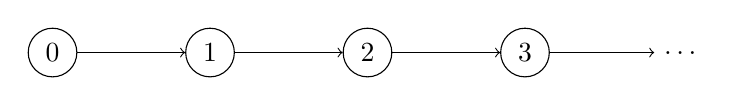
\begin{tikzpicture}
    \node (a) at (0,0) [circle, draw] {0};
    \node (b) at (2,0) [circle,draw] {1}; \node (c) at (4,0)
    [circle,draw] {2}; \node (d) at (6,0) [circle,draw] {3}; \node (e)
    at (8,0) {\ldots}; \draw[->] (a.east) -- (b.west); \draw[->]
    (b.east) -- (c.west); \draw[->] (c.east) -- (d.west); \draw[->]
    (d.east) -- (e.west);
  \end{tikzpicture}
  \caption{A picture of the natural numbers}
  \label{fig:nat-numbers}
\end{figure}


Not all ``stepping stone'' pictures are acceptable.
Figures \ref{fig:NatSigBad1}, \ref{fig:NatSigBad2} and \ref{fig:NatSigBad3} illustrate three ways \emph{not} to picture the natural numbers.

\begin{figure}[h]
\centering
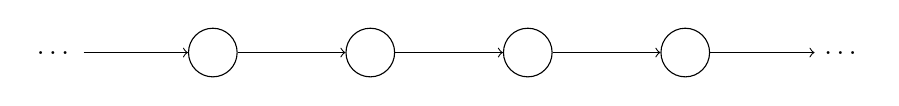
\begin{tikzpicture}
  \node (z) at (-2,0) {\ldots}; 
\node (a) at (0,0) [circle, draw] {\phantom0};
    \node (b) at (2,0) [circle,draw] {\phantom0}; \node (c) at (4,0)
    [circle,draw] {\phantom0}; \node (d) at (6,0) [circle,draw] {\phantom0}; 
    \node (e) at (8,0) {\ldots}; 
    \draw[->] (z.east) -- (a.west); \draw[->] (a.east) -- (b.west); \draw[->]
    (b.east) -- (c.west); \draw[->] (c.east) -- (d.west); \draw[->]
    (d.east) -- (e.west);
%\node (left) at (0,0) [circle,draw] {}; \node (center) at (1,0)
%  [circle,draw] {}; \node (right) at (2,0) [circle,draw] {}; \draw[<-]
%  (left.north east)--(center.north west); \draw[->] (center.south
%  east)--(right.south west); \draw[->] (left.south
%  east)--(center.south west); \draw[<-] (center.north
%  east)--(right.north west);
\end{tikzpicture}
\caption{Nowhere to start}\label{fig:NatSigBad1}

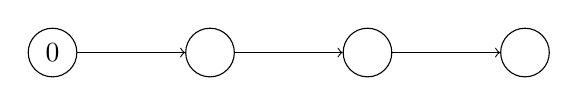
\begin{tikzpicture}
  \node (a) at (1,0) [circle, draw] {0};
    \node (b) at (3,0) [circle,draw] {\phantom0}; \node (c) at (5,0)
    [circle,draw] {\phantom0}; \node (d) at (7,0) [circle,draw] {\phantom0}; 
    \draw[->] (a.east) -- (b.west); \draw[->]
    (b.east) -- (c.west); \draw[->] (c.east) -- (d.west);
\end{tikzpicture}
\caption{Nowhere to go}\label{fig:NatSigBad2}

\begin{tikzpicture}
%    \node (a) at (0,0) [circle, draw] {0};
    \node (b) at (2,0) [circle,draw] {0}; 
    \node (c) at (4,0) [circle,draw] {\phantom0}; 
    \node (d1) at (6,1) [circle,draw] {\phantom0}; 
    \node (d2) at (6,-1) [circle,draw] {\phantom0}; 
    \node (e1) at (8,1) [circle,draw] {\phantom0}; 
    \node (e2) at (8,-1) [circle,draw] {\phantom0};
    \node (f) at (10,0) [circle,draw] {\phantom0};
    \node (g) at (12,0) {\ldots};
%    \draw[->] (a.east) -- (b.west); 
    \draw[->] (b.east) -- (c.west); 
\draw[->] (c.north east) -- (d1.west);
\draw[->] (c.south east) -- (d2.west);
\draw[->] (d1.east) -- (e1.west);
\draw[->] (d2.east) -- (e2.west);
\draw[->] (e1.south east) -- (f.west);
\draw[->] (e2.north east) -- (f.west);
\draw[->] (f.east) -- (g.west);
\end{tikzpicture}
\caption{Forks in the path}\label{fig:NatSigBad3}
\end{figure}

These incorrect pictures can be ruled out by explaining the basic structure of counting. We will ``explain the obvious'' by stating things like this as \emph{postulates}.

%\refstepcounter{axiomCnt}
\begin{postulate}[Basic Structure of Natural Numbers]\label{post:NatSig}
The \newterm{natural numbers} have the following basic structure.
  \begin{itemize}
  \item There is a special natural number. We denote this by $0$.
  \item For any natural number $n$, there is
    a unique \emph{next} natural number. We call this the \newterm{successor of $n$}. 
    In these lectures, we denote the successor of $n$ by $n^\nxt$.
  \end{itemize}
\end{postulate}

According to Postulate \ref{post:NatSig}, $0$, $0^\nxt$, $0^{\nxt\nxt}$, $0^{\nxt\nxt\nxt}$ each denote a natural number. 
Of course, we usually abbreviate them by writing $0$, $1$, $2$, $3$.
But the \emph{characters} $1$, $2$, $3$, etc., are not related to each other in any way.
The notation we are using here makes it completely clear that $0^\nxt$ is the number after $0$, and so on. 
We will want to be able to switch between the familiar ``decimal' notation and ``successor'' notation whenever it is convenient.

\begin{exer}
\begin{multicols}{2}
%\begin{itemize}
\item Convert the following from decimal notation to successor notation.
  \begin{exercise}
  \item $9$
  \item $10$
  \item $4 + 3$
  \item $n + 4$
  \end{exercise}
\item Convert the following to from successor notation to decimal notation.
\begin{exercise}
\item $0^{\nxt\nxt\nxt\nxt}$
\item $n^{\nxt\nxt\nxt\nxt\nxt}$
\item $5^{\nxt\nxt}$
\item $0^\nxt + 0^{\nxt\nxt}$
\end{exercise}
%\end{itemize}
\end{multicols}
\end{exer}

\printbreak

\section{Narrowing the possibilities}

Figures \ref{fig:one-loop} and \ref{fig:two-loop} illustrate 
problems that Postulate \ref{post:NatSig} does not avoid.

\begin{figure}[ht]
  \centering
  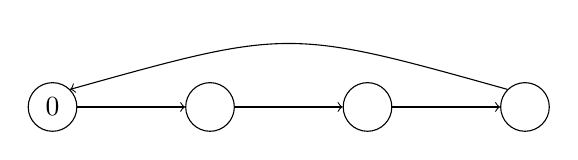
\begin{tikzpicture}
    \node (a) at (0,0) [circle, draw] {$0$}; \node (b) at (2,0)
    [circle,draw] {\phantom{$0$}}; \node (c) at (4,0) [circle,draw]
    {\phantom{$0$}}; \node (d) at (6,0) [circle,draw] {\phantom{$0$}};
    \draw[->] (a.east) -- (b.west); \draw[->] (b.east) -- (c.west);
    \draw[->] (c.east) -- (d.west); \draw[->] (d.north west)
    .. controls (3,1) .. (a.north east);
  \end{tikzpicture}
  \caption{A strange way to count}
  \label{fig:one-loop}
\end{figure}

\begin{figure}[ht]
  \centering
  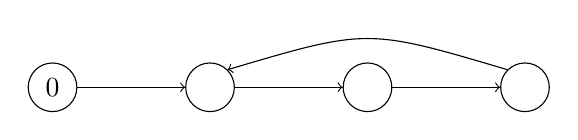
\begin{tikzpicture}
    \node (a) at (0,0) [circle, draw] {$0$}; \node (b) at (2,0)
    [circle,draw] {\phantom{$0$}}; \node (c) at (4,0) [circle,draw]
    {\phantom{$0$}}; \node (d) at (6,0) [circle,draw] {\phantom{$0$}};
    \draw[->] (a.east) -- (b.west); \draw[->] (b.east) -- (c.west);
    \draw[->] (c.east) -- (d.west); \draw[->] (d.north west)
    .. controls (4,.75) .. (b.north east);
  \end{tikzpicture}
  \caption{Another strange way to count}
  \label{fig:two-loop}
\end{figure}
\clearpage

\begin{exer}
\begin{exercise}
\item Explain, in one or two sentences each, why Figures \ref{fig:one-loop} and \ref{fig:two-loop} depict systems that agree with Postulate \ref{post:NatSig}.
\end{exercise}
\end{exer}
\ipadbreak

Figure \ref{fig:one-loop} is flawed because $0$ has a
\emph{predecessor}: a value $n$ satisfying $0^{\nxt\nxt\nxt\nxt} = 0$. Figure
\ref{fig:two-loop} is flawed because an element has two distinct
predecessors: $0^\nxt = 0^{\nxt\nxt\nxt\nxt}$.  We can insist that
these flaws do not happen in the natural numbers. That is, 
we rule them out with axioms.

\begin{postulate}{Nothing Precedes $0$}\label{post:NatZero}
  For every natural number $n$, $n^\nxt\neq 0$.
\end{postulate}

\begin{postulate}{Predecessors are Unique}\label{post:NatPred}
  For any natural numbers $m$ and $n$, if $m^\nxt=n^\nxt$ then $m=n$.
\end{postulate}

These postulates eliminate Figures \ref{fig:one-loop}, \ref{fig:two-loop} and similar pictures.  
But there is still a subtle problem. 
Consider Figure \ref{fig:nonstandard}.

\begin{figure}[h]
  \centering
  \begin{tikzpicture}
    \node (a) at (0,0) [circle, draw] {$0$}; \node (b) at (2,0)
    [circle,draw] {\phantom{$0$}}; \node (c) at (4,0) [circle,draw]
    {\phantom{$0$}}; \node (d) at (6,0) [circle,draw] {\phantom{$0$}};
    \node (e) at (8,0) {\ldots}; \draw[->] (a.east) -- (b.west);
    \draw[->] (b.east) -- (c.west); 
    \draw[->] (c.east) -- (d.west);
    \draw[->] (d.east) -- (e.west);
    % \node (z) at (0,2) {\ldots};
    \node (aa) at (2,2) [circle, draw] {$\star$}; \draw[->] (aa.east)
    .. controls (3.5,3) and (0.5,3) .. (aa.west);
    % \node (bb) at (4,2) [circle,draw] {\phantom{$0$}}; \node (cc) at
    % (6,2) [circle,draw] {\phantom{$0$}}; \node (dd) at (8,2)
    % [circle,draw] {\phantom{$0$}}; \node (ee) at (10,2) {\ldots};
    % \draw[->] (z.east) -- (aa.west); \draw[->] (aa.east) --
    % (bb.west); \draw[->] (bb.east) -- (cc.west); \draw[->] (cc.east)
    % -- (dd.west); \draw[->] (dd.east) -- (ee.west);
  \end{tikzpicture}
  \caption{A model of the natural numbers?}
  \label{fig:nonstandard}
\end{figure}

This picture satisfies the first three postulates. 
Yet, it is not a picture of natural numbers because it has ``extra stuff'' in it ($\star$).

\ipadbreak

To rule out ``extra stuff'', we formulate our final postulate for natural numbers.
We diagnose the problem as follows.
Were we to erase the circle labelled $\star$ and any the arrows leading to and from it, the remaining part of Figure \ref{fig:nonstandard} would still live up to Postulate \ref{post:NatSig}.
This is exactly what we mean by ``extra stuff'': 
elements that can be removed without violating the Postulate \ref{post:NatSig} (the essential structure). 
This leads to our last axiom. 

\begin{postulate}{The Axiom of Induction}\label{post:NatInd}
 No natural numbers can be removed without violating \ref{post:NatSig}.
\end{postulate}

%Believe it or not, the four axioms we have stated here completely
%characterize the standard picture of the natural numbers. In other
%words, any picture that satisfies these axioms will look the same. A
%rigorous proof of this is possible, but not necessary for now.

\begin{exer}
\begin{exercise}
\item Each of the following pictures fails to satisfy either the one or more of our axioms. 
For each, explain which axioms are violated.
\begin{multicols}{2}
\begin{enumerate}
\item
  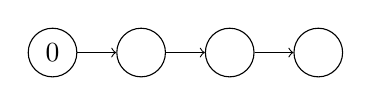
\begin{tikzpicture}[scale=.75]
    \node (a) at (0,0) [circle, draw] {$0$}; \node (b) at (1.5,0)
    [circle,draw] {\phantom{$0$}}; \node (c) at (3,0) [circle,draw]
    {\phantom{$0$}}; \node (d) at (4.5,0) [circle,draw] {\phantom{$0$}};
    \draw[->] (a.east) -- (b.west); \draw[->] (b.east) -- (c.west);
    \draw[->] (c.east) -- (d.west);
  \end{tikzpicture}
\item
  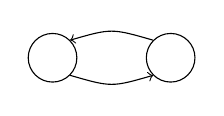
\begin{tikzpicture}[scale=.75]
    \node (a) at (0,0) [circle, draw] {\phantom{$0$}};
    \node (b) at (2,0) [circle, draw] {\phantom{$0$}};
    \draw[->] (a.south east) .. controls (1,-.5) .. (b.south west);
    \draw[->] (b.north west) .. controls (1,.5) .. (a.north east);
  \end{tikzpicture}
\item  
  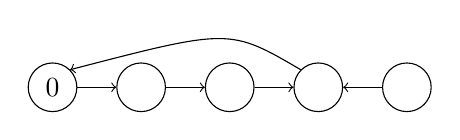
\begin{tikzpicture}[scale=.75]
    \node (a) at (0,0) [circle, draw] {$0$}; \node (b) at (1.5,0)
    [circle,draw] {\phantom{$0$}}; \node (c) at (3,0) [circle,draw]
    {\phantom{$0$}}; \node (d) at (4.5,0) [circle,draw] {\phantom{$0$}};
    \node (e) at (6,0) [circle,draw] {\phantom{$0$}};
    \draw[->] (a.east) -- (b.west); \draw[->] (b.east) -- (c.west);
    \draw[->] (c.east) -- (d.west); \draw[->] (d.north west)
    .. controls (3,1) .. (a.north east);
    \draw[->] (e.west) -- (d.east);
  \end{tikzpicture}
\item
  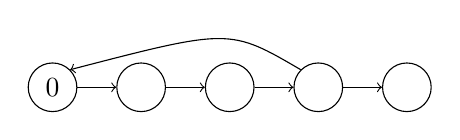
\begin{tikzpicture}[scale=.75]
    \node (a) at (0,0) [circle, draw] {$0$}; \node (b) at (1.5,0)
    [circle,draw] {\phantom{$0$}}; \node (c) at (3,0) [circle,draw]
    {\phantom{$0$}}; \node (d) at (4.5,0) [circle,draw] {\phantom{$0$}};
    \node (e) at (6,0) [circle,draw] {\phantom{$0$}};
    \draw[->] (a.east) -- (b.west); \draw[->] (b.east) -- (c.west);
    \draw[->] (c.east) -- (d.west); \draw[->] (d.north west)
    .. controls (3,1) .. (a.north east);
    \draw[->] (d.east) -- (e.west);    
  \end{tikzpicture}
\end{enumerate}
\end{multicols}

\item\label{exer:cases} I have in mind a picture for the Basic Vocabulary \ref{post:NatSig} and that satisfies Axioms \ref{post:NatZero}
and \ref{post:NatPred}. Furthermore, in that picture, I have in mind and element $n$ for which (a) $n\neq 0$
and (b) $n$ has no predecessor (that is, $n\neq m^\nxt$ for every $m$). Convince me that
the picture fails to satisfy Axiom \ref{post:NatInd}.
\item\label{exer:CyclicModel} Draw three different pictures of situations that satisfies all the postulates except that they fail Postulate \ref{post:NatZero}. So there will be an arrow from a bubble into the bubble $0$. The result must satisfy all other postulates including the Axiom of Induction.
\end{exercise}
\end{exer}

The latest exercise shows that in the natural numbers, if $n\neq 0$, then $n = m^\nxt$ for some $m$. In other
words, every non-zero natural number has a predecessor. 


\chapter{Arithmetic}\label{lec:Arithmetic}


\begin{goals}
\tightlists
\noindent\textbf{Lecture}
\begin{itemize}
\item Present addition and multiplication via defining equations.
\item Practice using the defining equations to calculate sums and products.
\end{itemize}

\noindent\textbf{Study}
\begin{itemize}
  \item Understand addition and multiplication as characterized by defining equations.
  \item Be able to explain how addition and multiplication relate to counting.
  \item Exhibit competence in calculating sums and products from the defining equations.
\end{itemize}
\defaultlists
\end{goals}

Adding and multiplying arise from counting. In this section, we explore how to define them purely in terms of counting.

\ipadbreak
\printbreak

\section{Basic Arithmetic Operations}

We know that addition ``works'' by counting ahead. For example, to \emph{add} $4+5$, we can start with $4$ and then count up five more. Likewise, multiplication ``works'' by counting a number of additions. For example, to multiply $2\cdot 3$ we can add $2$ three times: $2+2+2$. The following definitions capture the idea.
 
\begin{defn}[Arithmetic Operations]\label{def:NatArithmetic}
\noindent The \newterm{sum} of two natural numbers, $m$ and $n$, is a natural number (denoted by $m+n$). For every natural number $m$, the following 
are true:
\begin{align*}
    m + 0     &= m\\
    m + k^\nxt &= (m + k)^\nxt &&\text{for any natural number $k$}
\end{align*}

\noindent The \newterm{product} of two natural numbers, $m$ and $n$, is a natural number 
(denoted by $m\cdot n$). For every natural number $m$, the following are true:
\begin{align*}
  m\cdot 0 &= 0\\
  m\cdot k^\nxt &= m + (m\cdot k) &&\text{for any natural number $k$}
\end{align*}
\end{defn}


A moment's thought about arithmetic should convince you that these equations are reasonable.
Certainly $m+0=m$ and $m\cdot 0 = 0$ should be true for any $m$. 
The second equation for $+$ can be read as saying ``to add $m$ to the successor of $k$, simply add $m$ to $k$, then take the successor.''
The second equation for $\cdot$ can be read as saying ``to multiply $m$ by the successor of $k$, simply multiply $m$ by $k$, and add $m$ to the result.''

The Axiom of Induction ensures that there are indeed unique operations $+$ and $\cdot$ that satisfy the equations.
A proof of this fact is not particularly illuminating right now, so let us agree to take it for granted.

\begin{example}
Do the defining equations for addition really explain how to add? Let's use them to calculate
$4+3$:
\begin{align*}
  4 + 3 &= 4 + 0^{\nxt\nxt\nxt}&&\text{[$3$ abbreviates $0^{\nxt\nxt\nxt}$]}\\
  &= (4 + 0^{\nxt\nxt})^\nxt &&\text{[$m+k^\nxt = (m+k)^\nxt$]}\\
  &= (4 + 0^\nxt)^{\nxt\nxt} &&\text{[Same reason]}\\
  &= (4 + 0)^{\nxt\nxt\nxt} &&\text{[Same reason]}\\
  &= 4^{\nxt\nxt\nxt} &&\text{[$m+0 = m$]}\\
  &= (0^{\nxt\nxt\nxt\nxt})^{\nxt\nxt\nxt} && \text{[$4$ abbreviates $0^{\nxt\nxt\nxt\nxt}$]}\\
  &= 0^{\nxt\nxt\nxt\nxt\nxt\nxt\nxt} && \text{[Remove unneeded parentheses]}\\
  &= 7 &&\text{[$7$ abbreviates $0^{\nxt\nxt\nxt\nxt\nxt\nxt\nxt}$]}
\end{align*}
\end{example}
\ipadbreak

\begin{example}
A product can be calculated similarly. Consider $2\cdot 2$.
\begin{align*}
  2\cdot 2 &= 2\cdot 0^{\nxt\nxt} &&\text{[$2$ abbreviates $0^{\nxt\nxt}$]}\\
           &= 2 + (2\cdot 0^\nxt) &&\text{[$m\cdot k^\nxt = m + (m\cdot k)$]}\\
           &= 2 + (2 + (2\cdot 0))&&\text{[Same reason]}\\
           &= 2 + (2 + 0) &&\text{[$m\cdot 0=0$]}\\
           &= 2 + 2&&\text{[$m+0 = m$]}\\
           &= 2 + 0^{\nxt\nxt}&&\text{[$2$ abbreviates $0^{\nxt\nxt}$]}\\
           &= (2 + 0^\nxt)^\nxt &&\text{[$m+k^\nxt = (m+k)^\nxt$]}\\
           &= (2 + 0)^{\nxt\nxt}&&\text{[Same reason]}\\
           &= 2^{\nxt\nxt} &&\text{[$m+0 = m$]}\\
           &= (0^{\nxt\nxt})^{\nxt\nxt} &&\text{[$2$ abbreviates $0^{\nxt\nxt}$]}\\
           &= 0^{\nxt\nxt\nxt\nxt}&&\text{[Remove unnecessary parentheses]}\\
           &= 4 &&\text{[$4$ abbreviates $0^{\nxt\nxt\nxt\nxt}$]}
\end{align*}
\end{example}

We certainly will not want to calculate this way in real life. 
After all, it took twelve steps just to figure $2\cdot 2=4$. But these
examples and the following exercises show how addition and multiplication are
closely tied to simple counting. 

\ipadbreak

\begin{exer}
\begin{exercise}
\item Calculate these sums, following the previous example to write
  each step of your calculation explicitly. Include the reason for
  each step (as in the previous example).Take care to lay out the
  chain of equalities correctly, and do not skip any steps.
\begin{enumerate}
\item $2+4$
\item $4+2$
\item $3+(3+1)$
\item $(3+3)+1$
\item $0 + 3$
\end{enumerate}

\item Notice that it takes more steps to calculate $2+4$ than $4+2$, even though we know they will produce the same answer. Explain why.

\item Calculate the following values, writing each step explicity. 
 \begin{enumerate}
    \item $2\cdot 3$
    \item $0\cdot 2$
    \item $2\cdot(2\cdot 2)$
    \item $3\cdot(2 + 1)$
    \item $(3\cdot 2) + (3\cdot 1)$
    \end{enumerate}
\item Write a definition of exponentiation via defining equations. Follow the pattern
of definition I have written for addition and multiplication.
\end{exercise}
\end{exer}

\chapter{Laws of Arithmetic}\label{lec:ArithmeticLaws}

\begin{goals}
\noindent\textbf{Lecture}
\begin{itemize}
\item Present the most common Laws of Arithmetic for natural numbers.
\item Explain the method of \emph{proof by simple induction}
\item Prove a representative sample of the laws by simple induction.
\end{itemize}
\noindent\textbf{Study}
\begin{itemize}
\item Become familiar with the common names for the Laws of Arithmetic.
\item Pay particular attention to the Laws of Positivity and Cancellativity (they may be the least familiar to you).
\item Demonstrate the ability to identify the main parts of a proof by simple induction.
\item Demonstrate the ability to construct the parts of a proof by simple induction.
\item Prove the remaining laws for yourself.
\end{itemize}
\end{goals}

Before working the last exercises, you knew that $3\cdot (2+1)$ and $3\cdot 2+ 3\cdot 1$
would come out the same because of a law of arithmetic known as \emph{distributivity}. 
Addition and multiplication satisfy several other laws.

\ipadbreak
\printbreak

%\section{Basic Laws}

The following list summarizes several useful laws of
arithmetic on the natural numbers. They are organized to emphasize
similarities between addition and multiplication.

\begin{laws}
\noindent For any natural numbers, $m$, $n$ and $p$:

\begin{tabular}{lr@{\,}l}
\textbf{Associativity}& $m + (n + p)$       &$= (m+n)+p$\\
                      & $m \cdot(n\cdot p)$ &$= (m\cdot n)\cdot p$\\
\textbf{Commutativity}& $m + n$             &$= n + m$\\
                      &                     &$m\cdot n$ &$= n\cdot m$\\
&&\\ 
\textbf{Identity}     & $m + 0$             &$= m$\\
                      & $m\cdot 1$          &$= m$\\
&\textbf{Positivity}&\multicolumn{2}{c}{if $m + n = 0$ then $m=0$}\\
                                    &\multicolumn{2}{c}{if $m\cdot n = 1$ then $m=1$}\\
&&\\
\textbf{Cancellativity}&\multicolumn{2}{c}{if $m + p = n+p$ then $m=n$}\\
                       &\multicolumn{2}{c}{if $m \cdot p^\nxt = n\cdot p^\nxt$ then $m=n$}\\
&&\\
\textbf{Distributivity}&$m\cdot(n+p)$&$= (m\cdot n) + (m\cdot p)$\\
&&\\
\textbf{Case Distinction}&\multicolumn{2}{c}{if $m\neq 0$ then $m=k^\nxt$ for some $k$}\\
\end{tabular}
\end{laws}
\medskip

Most of these laws are familiar and are listed with their common names. The Law of Case
Distinction was the subject of Lecture \ref{lec:NatNumbers} Exercise \ref{exer:cases}. \emph{Go back and look at that exercise again}.
The Law of Positivity for multiplication is not a common name, but
I have used it to emphasize the analogies between addition and multiplication.
Also Case Distinction does not really have a common name. I made that up.

\ipadbreak

\section{Inductive Proofs}

Suppose we wish to prove that every natural number has some
property. For example, let us suppose we wish to prove that every
natural number is \emph{mimsy}.  I have no idea what a mimsy number
is, but let us try to prove this anyway. We could try proving that $0$
is mimsy, $1$ is mimsy, $2$ is mimsy, and so on.  But this won't work
because our proof will never end. In fact, it is not so obvious that
we, humans with finite minds, can ever prove that some property is
true for \emph{all} natural numbers, since it seems to involve
checking infinitely many individual cases.

The Axiom of Induction provides a way forward in spite of our
limitations.  Suppose we were to show that the mimsy natural numbers
all by themselves constitute a picture of Signature
\ref{post:NatSig}.  Then there could not be any natural numbers
left out, for otherwise, we could erase all the non-mimsy natural
numbers and still have a picture of \ref{post:NatSig}. This
is exactly what the Axiom of Induction forbids: we can not erase
\emph{anything} without breaking the signature.

So to prove that all natural numbers are mimsy, we simply need to
prove that
\begin{itemize}
\item $0$ is mimsy, and
\item for all natural numbers $k$, if $k$ is mimsy so is $k^\nxt$.
\end{itemize}
From these, we conclude that the mimsy natural numbers by themselves form a picture of \ref{post:NatSig}. So the Axiom of Induction ensures that all natural numbers
are mimsy.

%\begin{usage}
%  A proof employing the Axiom of Induction in this way is called a
%  proof \emph{by simple arithmetic induction}, or just a proof \emph{by
%    induction}, for short.  We will see more general forms of
%  induction later.
%\end{usage}

To make inductive proofs easier to understand, we often write them
using a three step outline, as illustrated here.
\begin{itemize}
\item{}[Basis] Prove that $0$ is mimsy.
\item{}[Inductive Hypothesis] Assume that $k$ is mimsy.
\item{}[Inductive Step] Prove that $k^\nxt$ is mimsy. [You may use the
  assumption that $k$ is mimsy in this part of the proof.]
\end{itemize}

More practical examples are next.

\begin{prop}

  \emph{Addition is associative.}

\begin{proof}
  We need to show that $m + (n+p) = (m+n)+p$ for all $m$, $n$ and $p$.
  Let us suppose that $m$ and $n$ are fixed values (not known to us).
  We now prove that the values $p$ for which $m+(n+p) = (m+n)+p$ holds
  form a picture of \ref{post:NatSig}.
  \begin{itemize}
  \item{}[Basis] $m+(n+0) = m+n = (m+n)+0$. Both steps are due to the
    defining equations of $+$.
  \item{}[Inductive Hypothesis] Assume $m+(n+k) = (m+n)+k$.
  \item{}[Inductive Step] We must show that $m+(n+k^\nxt) =
    (m+n)+k^\nxt$. 
    \begin{align*}
      m+(n+k^\nxt) &= m + (n+k)^\nxt &&\text{[Def. of +]}\\
      &= (m+(n+k))^\nxt&&\text{[Same]}\\
      &= ((m+n)+k)^\nxt&&\text{[Inductive Hypothesis]}\\
      &= (m+n)+k^\nxt &&\text{[Def. of $+$]}
    \end{align*}
  \end{itemize}
  Therefore (by the Axiom of Induction), $m+(n+p) = (m+n)+p$ holds for
  all $p$. Since the argument does not depend on any extra assumptions
  about $m$ and $n$, it holds for all $m$ and $n$.
\end{proof}
\end{prop}

\printbreak

In the remainder of this section, we further illustrate the technique of simple arithmetic induction via proofs of other laws of arithmetic.

\ipadbreak

\begin{prop}\label{prop:AddZero}
  $0$ is the identity for addition.

\begin{proof}
  We must prove that $m+0 = m = 0 + m$ for all $m$. The first equality is true by the definition of $+$.
  But the second equality, $m = 0 + m$, is not explicitly one of the defining facts about $+$. So we proceed by induction on $m$.
  \begin{itemize}
  \item{}[Basis] $0+0 = 0$ is true by definition of $+$.
  \item{}[Inductive Hypothesis] Assume $0 + k = k$.
  \item{}[Inductive Step] We must show that $0 + k^\nxt = k^\nxt$.
    \begin{align*}
      0 + k^\nxt &= (0+k)^\nxt &&\text{[Def. of $+$]}\\
      &= k^\nxt &&\text{[Inductive hypothesis]}
    \end{align*}
  \end{itemize}
  Therefore, $0+m=m$ holds for all $m$.
\end{proof}
\end{prop}

\ipadbreak

To prove that addition is commutative, we need an additional fact
about how successor and addition interact. 
Mathematicians use the word \emph{lemma} to indicate that a certain fact is only needed to make others proofs easier and is not necessarily valuable in its own right.

\printbreak

\begin{lem}\label{lem:AddSucc}
  For any $m$ and $n$, $(m + n)^\nxt = m^\nxt + n$.

 \begin{proof}
   By induction on $n$:
   \begin{itemize}
   \item{}[Basis]
     \begin{align*}
       (m + 0)^\nxt &= m^\nxt     &&\text{[Def. of $+$]}\\
       &= m^\nxt + 0 &&\text{[Def. of $+$]}
     \end{align*}
   \item{}[Inductive Hypothesis]
    Assume $(m + k)^\nxt = m^\nxt + k$ for some $k$.
   \item{}[Inductive Step]
    We must show that $(m + k^\nxt)^\nxt = m^\nxt + k^\nxt$.
    \begin{align*}
      (m + k^\nxt)^\nxt &= ((m + k)^\nxt)^\nxt && \text{[Def. of $+$]}\\
                     &= (m^\nxt + k)^\nxt &&\text{[Inductive Hypothesis]}\\
                     &= m^\nxt + k^\nxt   &&\text{[Def. of $+$]}
    \end{align*}
   \end{itemize}
So $(m + n)^\nxt = m^\nxt + n$. Because the proof does not depend on any assumption about $m$, it is valid
for all $m$.
 \end{proof}
\end{lem}

Roughly speaking this lemma permits us to move $\nxt$ anywhere within an addition: $m^\nxt + n = (m+n)^\nxt = m+n^\nxt$. So we are free to move a successor ``out of the way'' whenever we need to. The next proof illustrates the point.

\printbreak

\begin{prop}

  \emph{Addition is commutative.}

\begin{proof}
  We need to show that $m+n = n + m$ for all $m$ and $n$.  This time,
  the proof is by induction on $m$. Fix a value for $n$.
  \begin{itemize}
  \item{}[Basis] $0 + n = n = n + 0$ holds because of Proposition
    \ref{prop:AddZero} and the definition of $+$.
  \item{}[Inductive Hypothesis] Assume that $k + n = n + k$ for some
    $k$.
  \item{}[Inductive Step] We must show that $k^\nxt + n = n + k^\nxt$.
    \begin{align*}
      k^\nxt + n &= (k + n)^\nxt&&\text{[Lemma \ref{lem:AddSucc}]}\\
      &=  (n+k)^\nxt&&\text{[Inductive Hypothesis]}\\
      &= n + k^\nxt&&\text{[Def. of $+$]}
    \end{align*}
  \end{itemize}
  Therefore, $m + n = n + m$ for all $m$. Since this argument does not
  depend on any assumptions about $n$, it is valid for all $n$.
\end{proof}
\end{prop}

The next law may be less familiar to you. Roughly, it says that we can ``subtract'' equals and get equals. But note that actual subtraction does not always make sense for natural numbers. We can not, for example, say what $5-7$ means without introducing negative numbers.

\printbreak

\begin{prop}
  \emph{Addition is cancellative.}

\begin{proof}
  We need to prove that if $m + p= n+p$, then $m=n$.  This proof is a little subtler than the previous ones. But notice that is
  still follows the same form.
  
  The proof is by induction on $p$. Assume that $m$ and $n$ are some fixed natural numbers.
  \begin{itemize}
  \item{}[Basis] Suppose $m+0 = n+ 0$. Then immediately by definition
    of $+$, $m=n$.
  \item{}[Inductive Hypothesis] Assume that the following statement is true for some $k$: if $m + k = n + k$ then $m=n$.
  \item{}[Inductive Step] We must show that 
    if $m+k^\nxt = n+k^\nxt$ then $m=n$. Suppose $m+k^\nxt = n + k^\nxt$ [call this (*) for reference]. Then
    \begin{align*}
      (m+k)^\nxt & = m + k^\nxt &&\text{[Def. of $+$]}\\
      & = n + k^\nxt &&\text{[By the supposition (*)]}\\
      & = (n+k)^\nxt &&\text{[Definition of $+$]}
    \end{align*}
    Hence, by Axiom \ref{ax:NatPred} $m+k=n+k$. So by the Inductive Hypothesis, $m=n$.
  \end{itemize}
  Therefore, $m + p = n + p$ implies $m = n$ for all $p$. Since this argument does not
depend on any assumptions regarding $m$ and $n$, it is valid for all $m$ and $n$.
\end{proof}
\end{prop}
\ipadbreak

To prove that multiplication is commutative and cancellative, we will
need the following technical facts (analogous to Proposition
\ref{prop:AddZero} and Lemma \ref{lem:AddSucc}).

\begin{lem}\label{lem:MultZero}
  For any $n$, $0\cdot n = 0$

  \begin{proof}
    The proof is by induction on $n$.
    \begin{itemize}
    \item{}[Basis] $0\cdot 0 = 0$ by definition of $\cdot$.
    \item{}[Inductive Hypothesis] Assume that $0\cdot k = 0$ for some
      $k$.
    \item{}[Inductive Step] We must show that $0\cdot k^\nxt = 0$.
      \begin{align*}
        0\cdot k^\nxt &= 0 + 0\cdot k &&\text{[Definition of $\cdot$]}\\
        &= 0 + 0 &&\text{[Inductive Hypothesis]}\\
        &= 0&&\text{[Definition of $+$]}
      \end{align*}
    \end{itemize}
  \end{proof}
\end{lem}

\ipadbreak

\begin{lem}\label{lem:MultSucc}
  For any $m$ and $n$, $m^\nxt \cdot n = m\cdot n + n$

 \begin{proof}
   The proof is by induction on $n$.
   \begin{itemize}
   \item{}[Basis] $m^\nxt\cdot 0 = 0 = 0+0 = m\cdot 0 + 0$ all follow
     from the definitions of $+$ and $\cdot$.
   \item{}[Inductive Hypothesis] Assume that $m^\nxt\cdot k = m\cdot k +
     k$ for some $k$.
   \item{}[Inductive Step] We must show that $m^\nxt\cdot k^\nxt =
     m\cdot k^\nxt + k^\nxt$.
     \begin{align*}
       m^\nxt\cdot k^\nxt &= m^\nxt + m^\nxt\cdot k &&\text{[Exercise]}\\
       &= (m + m^\nxt\cdot k)^\nxt &&\text{[Exercise]}\\
       &= (m + (m\cdot k + k))^\nxt && \text{[Exercise]}\\
       &= ((m+ m\cdot k) + k)^\nxt &&\text{[Exercise]}\\
       &= (m\cdot k^\nxt + k)^\nxt &&\text{[Exercise]}\\
       &= m\cdot k^\nxt + k^\nxt &&\text{[Exercise]}
     \end{align*}
   \end{itemize}
 \end{proof}
\end{lem}

Some of the other laws are left as exercises.

\printbreak

\begin{exer}
  \begin{exercise}
\item Prove that $1$ is the identity for multiplication. That is $1\cdot m = m  = m\cdot 1$.
\item Write out the entire proof of Lemma \ref{lem:MultSucc} providing the justifications for each line of the equational calculation in the Inductive Step.
\item Prove that multiplication distributes over addition [$m\cdot
  (n+p) = m\cdot n + m\cdot p$] by induction on $p$.  You can use the any of the lemmas and propositions we have
  already proved.
  \begin{enumerate}
  \item Prove the basis: $m\cdot(n+0) = m\cdot n + m\cdot 0$.
  \item Write the inductive hypothesis.
  \item Prove the inductive step: $m\cdot(n+k^\nxt) = m\cdot n +
    m\cdot k^\nxt$
  \end{enumerate}
 
\item Prove that multiplication is associative [$m\cdot(n\cdot p) =
  (m\cdot n)\cdot p$] by induction on $p$.
  \begin{enumerate}
  \item Prove the basis: $m\cdot (n\cdot 0) = (m\cdot n)\cdot 0$.
  \item Write the inductive hypothesis.
  \item Prove the Inductive Step: $m\cdot (n\cdot k^\nxt) = (m\cdot
    n)\cdot k^\nxt$. 
    Hint: Use the Law of Distribution, which you just
    proved.
  \end{enumerate}

\item Prove that multiplication is commutative. 
Hint: Use the two Lemmas we proved right before these exercises.

  \end{exercise}
\end{exer}
%\ipadbreak
%
%For the record, we don't prove the cancellation law for multiplication here. It is similar to the others but a bit trickier. Nevertheless, the proof does not provide a new insight, so we omit it. 
%
%\begin{prop}
%
%  \emph{If $m\cdot p^\nxt = n\cdot p^\nxt$, then $m=n$.}
%
%\begin{proof}
%  The proof is by induction on $p$.
%  \begin{itemize}
%  \item{}[Basis] Suppose $m\cdot 0^\nxt = n\cdot 0^\nxt$. That is, $m\cdot 1=n\cdot 1$. Direct calculations show that $1$ is the identity for multiplication, so $m=n$. 
%  \item{}[Inductive Hypothesis] Assume that for some $k$, the following is true:
%    if $m\cdot k^\nxt = n\cdot k^\nxt$, then $m=n$.
%  \item{}[Inductive Step] Suppose that $m\cdot k^{\nxt\nxt} = n\cdot
%    k^{\nxt\nxt}$. Then
%    \begin{align*}
%      m\cdot k^{\nxt} + m &= k^\nxt\cdot p^\nxt &&\text{[By assumption]}\\
%      &= k\cdot p^\nxt + p^\nxt &&\text{[Lemma \ref{lem:MultSucc}]}\\
%      &= (k\cdot p^\nxt + p)^\nxt &&\text{[Definition of $+$]}\\
%      &\neq 0 &&\text{[Axiom Nat \ref{ax:NatZero}]}
%    \end{align*}
%    Consequently, $m\neq 0$, for otherwise we would have $m\cdot
%    p^\nxt = 0$. Since $m$ is not equal to $0$, it is equal to some
%    successor (by the Case Distinction Law). Let $j$ be the predecessor of $m$,
%	so that $j^\nxt=m$. Then
%    \begin{align*}
%      j\cdot p^\nxt + p^\nxt & = m\cdot p^\nxt &&\text{[Lemma \ref{lem:MultSucc}]}\\
%      &= k^\nxt \cdot p^\nxt &&\text{[By supposition]}\\
%      &= k\cdot p^\nxt + p^\nxt &&\text{[Lemma \ref{lem:MultSucc}]}
%    \end{align*}
%    Because addition is cancellative, $j\cdot p^\nxt = k\cdot
%    p^\nxt$. Now, the Inductive Hypothesis ensures that $j=k$. Hence
%    $m = j^\nxt = k^\nxt$.
%  \end{itemize}
%\end{proof}
%\end{prop}
	\chapter{Lists}

Natural numbers constitute an important example of something more
general, where objects are built up from simpler
ones. The Axiom of Induction captures the idea of building ``up''
and provides an important method for proving facts about natural
numbers.

In this lecture, we develop an analogous way to think about \emph{lists}. 

\begin{goals}
\noindent \textbf{Lecture Goals}
\begin{itemize}
\item Introduce a formal counterpart to the informal concept of a list
\item Emphasize the close analogy between lists and natural numbers
\item Introduce basic operations on lists.
\end{itemize}

\noindent\textbf{Study Goals}
\begin{itemize}
\item Demonstrate facility with basic list manipulation including calculating length and 
concatenation of lists.
\end{itemize}
\end{goals}

\section{List Basics}

In this section, we concentrate on the fundamental concept of \emph{lists}. The idea is really meant to
be the familiar one, so a list of ``to do'' items is a list. The alphabetized names on a class roster is a list. 
We will write lists using square brackets. So for example, $[2,3,5,7]$ is the list of 
the prime numbers less than $10$ in ascending order. For lists, we expect the order to matter. 
So $[7,5,3,2]$ is a different list.

Something that occurs on a list is called an \emph{item} of the list. We can even
specify where it is. So we can talk about the ``first'', ``second'' item, and so on, 
assuming the list has enough items. 

Because we have already agreed that natural numbers begin with $0$, it turns out to make
many things easier if we change the way we talk about items on a list to gibe with the natural
numbers. So instead of refering to the ``first'' item, we might call it the ``initial'' item.
Furthermore, we will number them to start with $0$. What I mean is that if $L=[2,3,5,7]$,
we will write $L_0$, $L_1$, $L_2$, $L_3$ for the elements $2$, $3$, $5$, $7$, respectively. 
In short, the ``initial'' item is indexed by the ``initial'' natural number $0$. The next item after that is indexed by next natural number, $0^\nxt$,
and so on.

Like natural numbers, lists can be built up by starting with an empty list and incrementally adding items. We have choices 
for how we might formalize the idea. We will follow a standard that has developed in computer science. Clearly, since we use 
square brackets to punctuate lists, the empty list should be written as $[\,]$. To add an item to a list, we will conventionally
put it on the front.  

Given the list $[x,y,z]$, we may build a new list with initial item $w$ and the given list as the rest, resulting in $[w,x,y,z]$.
The operation of \emph{prepending} an item to a list is denoted by a colon (:). 
So $w:[x,y,z]$ \emph{is} the list $[w,x,y,z]$.

The empty list, together with prepending items, gives us a way to construct any list we want.

\ipadbreak

\begin{example}
  Here are some examples.
  \begin{itemize}
  \item $5:6:[4,5]$ is the same as $5:[6,4,5]$, which is the same as
    $[5,6,4,5]$.
  \item $[\,]$ is the empty list
  \item $1:[\,]$ is the same as $[1]$
  \item $1:2:3:4:[\,]$ is the same as $[1,2,3,4]$.
  \end{itemize}
\end{example}

Notice that every list is either empty ($[\,]$) or not. If not, it has
the form $x:L$ where $x$ is the initial item and $L$
is the rest of the list. This suggests a signature for lists, not so different from
the signature for natural numbers.

\begin{postulate}[Basic Structure of Lists]\label{post:ListSig}
	Lists have the following basic structure.
	  \begin{itemize}
	  \item There is a special list, which we call \emph{the empty list} and denote by $[\,]$.
	  \item For any thing $x$ and any list $L$, there is another list, obtained by \emph{prepending} $x$ to $L$. We denote
	  the result by $x:L$.
	  \end{itemize}
\end{postulate}

As with the natural numbers, we need to think about axioms that prevent strange behavior. These are exactly analogous to the
axioms of natural numbers. First, $[\,]$ can not be obtained by adding a new initial item to another list. So

\begin{postulate}
	For any list $L$ and any thing $x$, $[\,]\neq x:L$.
\end{postulate}

Likewise, a list that is not empty can only be built one way.

\begin{postulate}
	For any things $x$ and $y$ and lists $L$ and $M$, if $x:L = y:M$, then $x=y$ and $L=M$.
\end{postulate}

For example, if I tell you that $[2,3,4,5] = x:L$, then you know immediately that $x=2$ and $L=[3,4,5]$.

Finally, lists need an induction axiom that ensures that all lists are built up from $[\,]$.


\begin{postulate}[The Axiom of List Induction]\label{post:ListInd}
	 No lists can be removed without violating Postulate \ref{sig:list}.
\end{postulate}

This axiom justifies conducting proofs about all lists by a scheme almost identical to simple arithmetic induction.
That is, to prove some property is true about all lists, it is enough to show
\begin{itemize}
\item{}[Basis] The property is true about $[\,]$.
\item{}[Inductive Hypothesis] Assume that the property is true for from list $K$.
\item{}[Inductive Step] Prove that for any thing $x$, the property is true about $x:K$. [You may use the
  assumption about $K$ in this part of the proof.]
\end{itemize}

Operations on lists can now also be defined by schemes similar to how 
we defined addition and multiplication on natural numbers. For example,
every list has a length. Writing $\len(L)$ for the length of a list,
$\len([2,3,4]) = 3$.  A precise definition is now easy to formulate.

\begin{defn}
  For a list $L$. the \emph{length} of $L$, denoted by $\len(L)$, is
  the natural number. This satisfies the following equalities.
  \begin{align*}
    \len([\,]) &= 0\\
    \len(x:L) &= len(L)^\nxt
  \end{align*}
\end{defn}

\begin{example}
  \begin{align*}
    \len([2,3,4]) &= \len(2:[3,4])\\
    &= \len([3,4])^\nxt\\
    &= \len(3:[4])^\nxt\\
    &= \len([4])^{\nxt\nxt}\\
    &= \len(4:[\,])^{\nxt\nxt}\\
    &= \len(,])^{\nxt\nxt\nxt}\\
    &= 0^{\nxt\nxt\nxt}\\
    &= 3
  \end{align*}
\end{example}

\ipadbreak

Another common operation on lists is \emph{concatenation}:
$[2,3,4]\otimes[4,1,3] = [2,3,4,4,1,3]$, whereby the two lists are simply glued together in their original orders.  This is defined precisely by
the following.

\begin{defn}
  For lists $L$ and $M$, their \emph{concatenation}, denoted by
  $L\otimes M$, is a list. For all lists $M$, the following are true.
  \begin{align*}
    [\,]\otimes M &= M\\
    (x:K)\otimes M &= x:(K\otimes M) & \text{for any thing $x$ and any list $K$}
  \end{align*}
\end{defn}

\begin{example}
  To calculate $[4,5,2,1] \otimes [3,4,1]$, we can follow a method similar to arithmetic:
  \begin{align*}
    [4,5,2,1]\otimes[3,4,1] &= (4:5:2:1:[\,])\otimes[3,4,1] & \text{[$[4,5,2,1]$ abbreviates $4:5:2:1:[\,]$]}\\
                    &= 4:((5:2:1:[\,])\otimes[3,4,1]) &\text{[Def. of $\otimes$]}\\
                    &= 4:5:((2:1:[\,])\otimes[3,4,1]) & \text{[Same]}\\
                    &= 4:5:2:((1:[\,])\otimes[3,4,1]) &\text{[Same]}\\
                    &= 4:5:2:1:([\,]\otimes[3,4,1])  &\text{[Same]}\\
                    &= 4:5:2:1:[3,4,1] &\text{[Same]}\\
                    &= [4,5,2,1,3,4,1]                &\text{[Abbreviation]}
  \end{align*}
\end{example}

\ipadbreak
Now we can prove some useful facts about lists.

\begin{lemma}
  On lists, $[\,]$ is the identity for $\otimes$,

\begin{proof}
  By definition
  $[\,]\otimes L = L$ always true.  But $[\,]$ must also 
  satisfy
  $L\otimes[\,] = L$ always. We can proceed by
  induction on $L$. The proof should look familiar (see the proof of
  Lemma \ref{lem:AddZero}).

  \begin{itemize}
  \item{}[Basis] $[\,]\otimes [\,] = [\,]$ is true by definition of
    $\otimes$.
  \item{}[Inductive Hypothesis] Assume $K\otimes[\,] = K$ for some list
    $K$.
  \item{}[Inductive Step]  Suppose $x$ is some thing. We need to show that $(x:K) \otimes [\,] = x:K$. 
    \begin{align*}
       (x:K)\otimes [\,] &= x:(K\otimes[\,]) &\text{[by definition of $\otimes$]}\\
	                   &= x:K &\text{[by the Inductive Hypothesis]}   	
    \end{align*}
  \end{itemize}
  Thus (by the Axiom of List Induction), the lists for which $L\otimes [\,] = L$ constitute all lists.
\end{proof}
\end{lemma}


\ipadbreak

\begin{lemma}
On lists, $\otimes$ is associative.

\begin{proof}
We prove $L\otimes(M\otimes N) =
  (L\otimes M)\otimes N$ using induction on $L$. This should look
  familiar. It is almost identicial to the proofs that addition and
  multiplication are associative.

  \begin{itemize}
  \item{}[Basis] $[\,]\otimes(M\otimes N) = M\otimes N = ([\,]\otimes M)\otimes
    N$. Both steps are by the definition of $\otimes$.
  \item{} [Inductive hypothesis] Suppose $K\otimes(M\otimes N) = (K\otimes
    M)\otimes N$ for some particular list $K$.
  \item{} [Inductive step]
    \begin{align*}
      (x:K)\otimes (M\otimes N) &= x:(K\otimes (M\otimes N)) &\mbox{Def. of $\otimes$}\\
      &= x:((K\otimes M)\otimes N) &\mbox{Inductive Hypothesis}\\
      &= (x:(K\otimes M))\otimes N &\mbox{Def. of $\otimes$}\\
      &= ((x:K)\otimes M)\otimes N &\mbox{Def. of $\otimes$}
    \end{align*}
  \end{itemize}
  So $L\otimes(M\otimes N) = (L\otimes M)\otimes N$ is true for all $L$. Since the proof
  does not depend on any special propertis of $M$ and $N$ (except that they are both lists),
  the result is true for all lists $M$ and $N$.
\end{proof}
\end{lemma}

\ipadbreak

Here is another nice fact that we can prove by induction relating
length to concatenation.

\begin{lemma}
  For any lists $L$ and $M$, $\len(L\otimes M) = \len(L)+\len(M)$.

\begin{proof} [This claim is probably fairly obvious to
  you. Nevertheless, to illustrate the technique of list
  induction again, we prove it explicitly.]
  \begin{itemize}
  \item {}[Basis] $\len([\,]) + \len(M) = 0 + \len(M) = \len(M) =
    \len([\,]\otimes M)$. These are by definition of $\otimes$ and $+$.
  \item{} [Inductive Hypothesis] Suppose $\len(K\otimes M) = \len(K)
    + \len(M)$ holds for some particular list $K$.
  \item{} [Inductive Step]
    \begin{align*}
      \len((x:K)\otimes M) &= \len(x:(K\otimes M)) &\mbox{Def. of $\otimes$}\\
      &= \len(K\otimes M)^\nxt &\mbox{Def. of $\len$}\\
      &= (\len(K)+\len(M))^\nxt &\mbox{Inductive Hypothesis}\\
      &= \len(K)^\nxt + \len(M) &\mbox{Lemma \ref{lem:AddSucc}}\\
      &= \len(x:K) + \len(M) &\mbox{Def. of $\len$}
    \end{align*}
  \end{itemize}
\end{proof}
\end{lemma}

Often we will use a list somewhat informally without all the
punctuation. For example, we might say ``Consider a list $a_0$, $a_1$,
\ldots, $a_{n-1}$ of real numbers.'' If we do not intend to use the list
itself for anything special, but only want to think about the numbers
$a_0$ through $a_n$, then there is no need to be formal about
it. Also, there is no harm in writing something like this: $a_5$,
$a_6$, $a_7$, $a_8$, where the indices start at
$5$. The default is to start at $0$, but that is merely a convention.

\begin{lemma}\label{lem:concat-cancellative}
$\otimes$ is cancellative on the left and on the right. That is,
\begin{itemize}
	\item $L\otimes M = L\otimes N$ implies $M=N$; and
	\item $L\otimes N = M\otimes N$ implies $L=M$.
\end{itemize}	

\begin{proof}
	Exercise.
\end{proof}
\end{lemma}

\section{List Itemization}

In a list $L$, the items are in order. So we can refer to items by
their position in the list. There are two standards in mathematics
for doing this. Either we start counting from $1$ or from $0$.
Although it may seem unintuitive at first to start from $0$ (meaning that
the ``initial'' item of a list is item number $0$), this actually 
makes many calculations simpler. For that reason, most programming
languages use this convention for a lists and arrays. So I will consistently
start with $0$.

The idea can be made precise as follows.

\begin{defn}\label{def:ListIndices}
Suppose $L$ is a list and $i<\len(L)$. Then $L_i$ is an item on the list
defined as follows.
\begin{align*}
  [\,]_i &\text{is never defined because $0\not<\len([\,])$}\\
  (x:L)_0 &= x\\
  (x:L)_{k^\nxt} &= L_k &\text{provided that $L_k$ is defined}
\end{align*}
\end{defn}

This is a precise way of explaining that in a list, for example $L=[a,b,c,d,e]$,
we can refer to an item by its \emph{index}, so that $L_0 = a$, $L_1=b$ and so on,
up to $L_4 = e$. Notice that $L_k$ is undefined if $k\geq \len(L)$.

\ipadbreak

\begin{example}
Suppose $L=[a,b,c,d,e]$. We can calculate $L_3$ 
explicitly step by step.
\begin{align*}
L_3 &= [a,b,c,d,e]_3\\
    &= (a:b:c:d:e:[\,])_{0^{\nxt\nxt\nxt}}\\
    &= (b:c:d:e:[\,])_{0^{\nxt\nxt}}\\
    &= (c:d:e:[\,])_{0^\nxt}\\
    &= (d:e:[\,])_0\\
    &= d
\end{align*}

Of course, this is just a very careful (you might even say fussy) way to find item number $3$ in the list. 
In every day use, we humans would not do this. 
We would simply count forward
from the beginning of the list.

\end{example}

\ipadbreak

\begin{exer}
	\begin{exercise}
 % \item Suppose $L$ is a list and $i<\len(L)$. Then it makes sense to 
  %      think about the list in which $L_i$ is removed. For example,
   %     for $L = [a, b, c]$, removing $L_1$ results in the list $[a,c]$.
    %    Let us denote the result of removing item $i$ from list $L$ as
     %   $L\setminus i$. So $[a,b,c]\setminus i = [a,c]$.

    %    In this exercise, you define $L\setminus i$ explicitly. Explain your answers for each point.
    %    \begin{enumerate}
    %    \item Should $[\,]\setminus 0$ be defined? If not, why not? If so, what should it be?
    %    \item What should $(x:L)\setminus 0$ be?
    %    \item What should $(x:L)\setminus k^\nxt$ be? When should it be defined and undefined?
    %    \item Now write your definition for $L\setminus i$ in a layout similar to Definition \ref{def:ListIndices}.
    %    \end{enumerate}
  \item Suppose $L = [3,2,3,3,5]$ and $M = [0,1,2,3,4,5]$. Calculate the following explicitly step by step.
  \begin{enumerate}
  \item $\len(L)$
  \item $L_4$
  \item $(L\otimes M)_9$
%  \item $L\setminus 4$.
%  \item $((M\otimes L)\setminus 3)_5$
  \end{enumerate}
\end{exercise}
\end{exer}

\ipadbreak

\section{Lists of a Particular Type}

We will commonly need to consider lists in which all elements are similar, such as a list consisting of natural numbers. For example,
because we know how arithmetic operations work on natural numbers, we can also define operations on lists of natural numbers using 
arithmetic. Similar extensions are possible for other operations defined on other types of elements.

To illustrate, suppose $L$ is a list of natural numbers. We can define the \emph{sum} of items on the list
in the obvious way, so that the sum of the list $[2,3,4]$ is $2+3+4 = 9$. We make this precise with the following.

\begin{defn}
	For a list $L$ of natural numbers, the \emph{sum of $L$}, denoted by $\sum L$, is a natural number, satisfying
	\begin{align*}
	\sum[\,] &= 0\\
	\sum m:L &= m + \sum L &\text{for any natural number $m$ and any list of natural numbers $L$}
	\end{align*}
\end{defn}

We will introduce variations and extensions of this notation this later. For now, we look only at lists. 

\begin{exer}
	\begin{exercise} 
\item Prove using list induction that for any lists of natural numbers,
\[\sum L + \sum M = \sum (L\otimes M)\]
\item Define the product of lists of natural numbers, following the pattern of our definition for $\sum L$. The standard notation
for a product is $\prod L$. The result should be that $\prod[2,3,4]$ equals $24$. Pay close attention the base case $\prod[\,]$.
\item Using your definition of products, prove by list induction that for any lists of natural numbers,
\[\prod L\cdot \prod M = \prod(L\otimes M)\]. 
\end{exercise}
\end{exer}

We can also consider lists of integers, lists of real numbers, and so on. We can even think about lists of lists.
For example, $[[2,3,4],[4,3,2],[5]]$ is a list consisting of two items: $[2,3,4]$, $[4,3,2]$ and $[5]$. Written this using
:, this is list is $[2,3,4]:[4,3,2]:[5]:[\,]$. Suppose we have a list of lists like this we can define the
concatenation of all the items. For this example, the result should be $[2,3,4,4,3,2,5]$. The definition of this
is exactly analogous to sums and products.

\begin{defn}
	For a list $\mathcal L$ of lists, the \emph{fold of $\mathcal L$}, denoted by $\bigotimes \mathcal L$, is a list, satisfying
	\begin{align*}
	\bigotimes[\,] &= [\,]\\
	\sum M:\mathcal L &= M \otimes \otimes \mathcal L &\text{for any list $M$ and any list of lists $\mathcal L$}
	\end{align*}
\end{defn}

Compare the definitions of $\sum$, $\prod$ and $\otimes$. They differ only in terms of (i) what is the result for an empty list
and (ii) what binary operation is used in the second equation.

Suppose we are given a list $\mathcal L$ of lists of natural numbers (like the example just above the latest definition). Then its fold is a list of natural numbers. So this can be summed. That is, $\bigotimes \mathcal L$ is a list of natural numbers, and $\sum(\otimes \mathcal L)$ is a natural number. But we might also apply the summation operation to each list on $\mathcal L$ separately, resulting in another list of natural numbers.
The idea of applying an operation to each element of a list is called ``mapping''. In this case, we intend to ``map'' the operation $\sum$
across lists of lists of natural numbers. Here is a suitable definition.

\begin{defn}
	For a list $\mathcal L$ of lists of natural numbers, the \emph{mapping of $\sum$
		 on $\mathcal L$}, denoted by $\map_{\sum}(\mathcal L)$
	is a list of natural numbers, satisfying
	\begin{align*}
	\bigotimes[\,] &= [\,]\\
	\sum M:\mathcal L &= ()\sum M): \mathcal L &\text{for any list of natural numbers $M$ and any list of lists of natural numbers $\mathcal L$}
	\end{align*}
\end{defn}

\begin{exer}
	\begin{exercise} 
	\item Calculate $\sum(\otimes[[3,4,5],[6,3]])$.
	\item Calculate $\map_{\sum}([[3,4,5],[6,3]])$.
	\item Calculate $\sum(\map_{\sum}([[3,4,5],[6,3]]))$.
	\item Prove that $\sum(\otimes\mathcal L) = \sum(\map_{\sum}(\mathcal L))$ for any list of lists of natural numbers $\mathcal L$.
	\end{exercise}
\end{exer}


\section{Other Inductively Defined Collections}

The structure of natural numbers and the structure of lists are very similar. This similarity can be exploited to 
develop a simple way of summarizing their properties.

For natural numbers, $0$ and $n^\nxt$ are the only ways to construct
them. Operations like addition and multiplication are
defined in terms of $0$ and ${}^\nxt$, so they do not contribute directly
to the \emph{construction} of natural numbers. So
we refer to $0$ and $\nxt$ as \emph{constructors}.

Axioms \ref{ax:NatZero} and \ref{ax:NatPred} spell out how these
constructors behave.  Namely, Axiom \ref{ax:NatZero} captures the idea that
the two constructors are entirely different from the other: $0\neq n^\nxt$.
Axiom \ref{ax:NatPred} captures the idea that ${}^\nxt$ constructs
distinct natural numbers from distinct natural numbers: $m^\nxt =
n^\nxt$ implies $m=n$ (or equivalently, $m\neq n$ implies $m^\nxt\neq n^\nxt$).

So the basic ingredients of natural numbers are the constructors $0$
and ${}^\nxt$ with the understanding that (a) each produces
different results and (b) from different ingredients, ${}^\nxt$
produces different results. In fact, point (b) also applies to $0$
trivially, because $0$ does not use any ingredients.

We can summarize everything we want to say about natural numbers
concisely in the following way.

\begin{defn}
  The \emph{natural numbers} are defined \emph{inductively} by
  \begin{align*}
    n &\defeq 0 \mathrel{\mid} n^\nxt
  \end{align*}
\end{defn}

In this notation, the vertical bar separates the different constructors for
natural numbers.  The first constructor ($0$) does not depend on
anything else. The second constructor depends on a natural number $n$
and produces a new one $n^\nxt$. So this gives a very concise description of the signature of natural numbers.
Implicitly, this notation is meant to
indicate that the two alternatives are completely distinct. This is
Axiom \ref{ax:NatZero}.  Also implicitly, the notation is meant indicate that $n^\nxt$
produces distinct results from distinct $n$'s.  This is Axiom
\ref{ax:NatPred}.  By declaring saying that this defines natural numbers
\emph{inductively}, we also mean that no natural numbers can be removed without violating
the signature.

Now let's consider lists. Again, there are two ways to construct lists. $[\,]$ and $x:L$ for any thing $x$
and any list $L$. Likewise, the constructrs are distinct, and $x:L=y:M$ is true if and only if
both $x=y$ and $L=M$. So we can encapsulate the definition of lists similarly.

\begin{defn}
    The \emph{lists} are defined \emph{inductively} by
    \begin{align*}
      L &\defeq [\,] \mathrel{\mid} x:L & \text{for any thing $x$}
    \end{align*}
\end{defn}

Notice that $x$ can also be a list.

Later in the course, we will make these definitions, and many others like them, rigorous.
For now, we just draw attention to the similarity between natural numbers and lists, and point out that proofs by induction work thanks to the structure of these definitions.



\section{Binary Trees}

\newcommand{\sz}{\mathord{\textsf{sz}}}
\newcommand{\hght}{\mathord{\textsf{ht}}}

\emph{Simple binary trees} are structures that play a role in many parts of computer science and mathematics.
Figure \ref{fig:BinTree} illustrates an example. There are many variations on the basic idea, but we concentrate
on the simplest version (where there is no extra structure).

\begin{figure}[h]
  \centering
\begin{tikzpicture}
[level/.style={sibling distance = 2cm/#1, level distance = 1.5cm}]
\node {}
child {node  {}
       child {node {$\bullet$}
              child {node {$\bullet$}}
              child {node {$\bullet$}}}
       child {node {$\bullet$}}
      }
child {node  {}
       child {node {$\bullet$}}
       child {node {$\bullet$}}
      };
\end{tikzpicture}
    
  \caption{A simple binary tree}
  \label{fig:BinTree}
\end{figure}

Such structures are built from \emph{leaves} (denoted here by $\bullet$) by ``grafting'' two smaller trees 
to form a larger one
as pictured in Figure \ref{fig:BinTreeConstruction}. Trees are usually depicted ``upside down'', so the \emph{root} is at the top and the leaves are at the bottom. What can you do? It's tradition. 
 

\begin{figure}[h]
  \centering
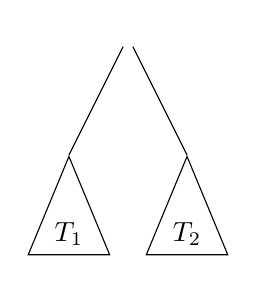
\begin{tikzpicture}
\usetikzlibrary{shapes.geometric}
\node {} [child anchor = apex]
child {node[draw, thin, isosceles triangle, anchor = apex, shape border rotate = 90]{$T_1$}}
child {node[draw, thin, isosceles triangle, anchor = apex, shape border rotate = 90]{$T_2$}};
\end{tikzpicture}

  \caption{Constructing a tree from subtrees}
  \label{fig:BinTreeConstruction}
\end{figure}

In addition to drawing pictures of binary trees, we can use a linear notation (something that can we written 
in the midst of prose). 
If $T_1$ and $T_2$ are simple binary trees, we may denote the tree constructed by grafting $T_1$ on the left and $T_2$ on the right
as $(T_1\curlywedge T_2)$ (as in Figure \ref{fig:BinTreeConstruction}. Thus we define simple binary trees, and two operations
on them, as follows.

\begin{defn}
\emph{Simple binary trees} are defined inductively by
\[T \defeq \bullet \,\mid\, (T_1\curlywedge T_2)\]
\end{defn}

The \emph{size} of a simple binary tree is a natural number defined by the equations
\begin{align*}
  \sz(\bullet) &\defeq 0\\
  \sz(T_1\curlywedge T_2) &\defeq 1 + \sz(T_1) + \sz(T_2)
\end{align*}
The \emph{height} of a simply binary tree a natural number is defined
by the equations
\begin{align*}
  \hght(\bullet) &\defeq 0\\
  \hght(T_1\curlywedge T_2) &\defeq 1 + \max(\hght(T_1),\hght(T_2))
\end{align*}
where $\max(m,n)$ is the larger of the two numbers.

These definitions suggest a relation between the size and height of a tree.
\ipadbreak

\begin{lemma}
For any simple binary tree $T$,  \[\hght(T)\leq \sz(T) < 2^{\hght(T)}.\]

\begin{proof}
To prove this by \emph{structural induction}, we must prove it for the basis ($\bullet$)
and that if it is true for some $T_1$ and $T_2$, then it is true for $(T_1\wedge T_2)$.
\begin{itemize}
\item{}[Basis] $\hght(\bullet) = 0$, $\sz(\bullet) = 0$ 
and $2^{\hght(\bullet)} = 1$. So the claim is true for $\bullet$.
\item{}[Inductive Hypothesis] Suppose the inequalities holds for some $T_1$ and $T_2$.
\item{}[Inductive Step] We must prove the two inequalities for $T= (T_1\curlywedge T_2)$.
Without loss of generality, assume that $\hght(T_1)\leq \hght(T_2)$. That is, if 
this is not so, then we may swap $T_1$ for $T_2$ in the following. 
\begin{align*}
\hght(T) &= 1 + \max(\hght(T_1),\hght(T_2)) &&\text{[Definition of $\hght$]}\\
         &\leq 1 + \hght(T_1) + \hght(T_2)  &&\text{[Arithmetic]}\\
         &\leq  1 + \sz(T_1) + \sz(T_2) &&\text{[Inductive Hypothesis]}\\
         &= \sz(T) &&\text{[Definition of $\sz$]}
       \end{align*}
And
\begin{align*}
\sz(T) &= 1 +\sz(T_1) + \sz(T_2)&&\text{[Definition of $\sz$]}\\
       &\leq 1 + 2^{\hght(T_1)} - 1) + (2^{\hght(T_2)} - 1)&&\text{[Inductive Hypothesis]}\\
       &\leq 2\cdot 2^{\hght(T_2)} - 1&&\text{[Assumption that $\hght(T_1)\leq \hght(T_2)$]}\\
       &= 2^{\hght(T_2)+1} - 1 &&\text{[Arithmetic]}\\
       &= 2^{\hght(T)} - 1 &&\text{[Definition of $\hght$]}
     \end{align*}
So $\sz(T) < 2^{\hght(T)}$
   \end{itemize}
 \end{proof}  
\end{lemma}

\ipadbreak

\begin{exer}
	\begin{exercise}
  \item Calculate the height and size of the following simple binary trees.
    \begin{enumerate}
    \item $(\bullet\curlywedge\bullet)$
    \item $(\bullet\curlywedge (\bullet\curlywedge\bullet))$
    \item $((\bullet\curlywedge\bullet)\curlywedge(\bullet\curlywedge(\bullet\curlywedge\bullet)))$
    \item $((\bullet\curlywedge(\bullet\curlywedge\bullet))\wedge ((\bullet\curlywedge\bullet)\curlywedge(\bullet\curlywedge(\bullet\curlywedge\bullet))))$
    \end{enumerate}
   \item Draw diagrams (similar to those in Figure \ref{fig:BinTree}) for the following
   simple binary trees.
   \begin{enumerate}
   \item $((\bullet \curlywedge \bullet)\curlywedge(\bullet\curlywedge\bullet))$
   \item $(((\bullet\curlywedge\bullet)\curlywedge\bullet)\curlywedge ((\bullet\curlywedge\bullet)\curlywedge(\bullet\curlywedge(\bullet\curlywedge\bullet))))$
   \end{enumerate}
   \item For each of the following diagrams, write the expression using $\bullet$ and $\curlywedge$
    defining the same tree.
\begin{multicols}{2}
    \begin{enumerate}
    \item 
\begin{tikzpicture}
\node {}
child {node {$\bullet$}}
child {node  {}
       child {node {$\bullet$}}
       child {node {$\bullet$}}
      };
\end{tikzpicture}

 \item 

\begin{tikzpicture}
[level/.style={sibling distance = 2cm/#1, level distance = 1.5cm}]
\node {}
child {node  {}
       child {node {$\bullet$}}
       child {node {$\bullet$}}
      }
child {node  {}
       child {node {$\bullet$}}
       child {node {$\bullet$}}
      };
\end{tikzpicture}

\item

\begin{tikzpicture}
\node {}
child {node  {}
       child {node {} 
              child {node {$\bullet$}}
              child {node {$\bullet$}}}
       child {node {$\bullet$}}
      }
child {node  {$\bullet$}};
\end{tikzpicture}

    \end{enumerate}
  \end{multicols}
  \end{exercise}
\end{exer}

We will study binary trees in more depth later in the course.

%
%
%\begin{exercise}
%\newcommand{\unit}{\mathord{\textbf{u}}}
%\newcommand{\B}{\mathord{\textbf{B}}}
%\newcommand{\C}{\mathord{\textbf{C}}}
%\newcommand{\denotation}{\mathord{\textsf{val}}}
%
%A \emph{widget} is defined inductively by
%\[M \defeq \unit \mid M\B \,\mid\, M\C\]
%
%For two widgets $M$ and $N$, their
%\emph{merge} is a widget, denoted by $M\oplus N$, defined by
%\begin{align*}
%\unit \oplus \unit &\defeq \unit\B\\
%\unit \oplus N\B &\defeq N\C\\
%\unit \oplus N\C &\defeq (\unit \oplus N)\B\\ 
%M\B \oplus \unit &\defeq M\C\\
%M\B \oplus N\B &\defeq (M\oplus N)\B\\
%M\B \oplus N\C &\defeq (M\oplus N)\C\\
%M\C \oplus \unit &\defeq  (M\oplus \unit)\B\\
%M\C \oplus N\B&\defeq (M\oplus N)\C\\
%M\C \oplus N\C&\defeq ((M\oplus N) \oplus \unit)\B
%\end{align*} 
%
%For a widget $M$, its \emph{value} is a natural number, denoted by
%$\llbracket M\rrbracket$, defined by
%\begin{align*}
%  \llbracket\unit\rrbracket &\defeq 1\\
%  \llbracket M\B\rrbracket &\defeq 2\cdot \llbracket M\rrbracket\\
%  \llbracket M\C\rrbracket &\defeq 2\cdot \llbracket M\rrbracket + 1
%\end{align*}
%
%Show that $\llbracket M\rrbracket + \llbracket N\rrbracket = \llbracket M\oplus N\rrbracket$ for any two
%widgets $M$ and $N$.
%\end{exercise}

%%% Local Variables: 
%%% mode: latex
%%% TeX-master: "MainText"
%%% End: 

	\chapter{Ordering the Natural Numbers by Addition}

We have used the ordering of numbers informally without much comment
because $\leq$ has its obvious meaning. In this lecture 
we exploit the fact that $\leq$ on the natural numbers is defined by addition, setting the stage for an
analogous concept defined by multiplication. The multiplicative
analogue of ``$m$ is less than or equal $n$'' is ``$m$ divides $n$''.

\begin{goals}
\begin{goal}{Lecture}
\item Introduce a formal definition of $\leq$ on natural numbers, and discuss simple facts about order
%\item Introduce formal definitions $\min$ and $\max$ as dual concepts
\item Review basic laws involving $\min$ and $\max$.
\item Introduce Strong Induction and the Principle of Well-foundedness as alternatives to Simple Induction.
\end{goal}

\begin{goal}{Study}
\item Prove basic facts about $\leq$, $\min$ and $\max$.
\item Commit to memory the concepts of reflexivity, transitivity, anti-symmetry and linearity.
\item Practice using Strong Induction.
\end{goal}
\end{goals}


\section{Less or Equal}

For the natural numbers, $\leq$ has a particularly simple definition.

\begin{defn}
  For natural numbers $n$ and $m$, say that \emph{$m$ is less than or equal to $n$} (written $m\leq n$)
  if and only if there is a
  natural number $d$ so that $m+d = n$.  [I've used the letter $d$
  because $d$ is the \emph{difference} of $m$ from $n$.]
  
  Also, say that \newterm{$m$ is (strictly) less than $n$} if and only if there is a natural number $d$ so that $m + d^\nxt = n$.
\end{defn}

All of the usual properties of $\leq$ for natural numbers follow
easily from this definition using only the laws of
addition. The important properties have names.

\begin{laws} 
\begin{description}
	\item[Reflexivity] $\leq$ is \emph{reflexive}: $m\leq
m$ is true for any $m$. This is simply because because $m + 0 =
m$. 
    \item[Transitivity] $\leq$ is \emph{transitive}: if $m\leq
n$ and $n\leq p$, then $m\leq p$. Transitivity follows from the law of
associativity for addition (you will prove this as an exercise).
    \item[Anti-symmetry] $\leq$ is \emph{anti-symmetric}: if $m\leq n$ and $n\leq m$, then
	$m=n$. This follows from cancellativity and positivity (another exercise).
	\item[Linearity] $\leq$ is \emph{linear}: for any $m$ and $n$, either $m\leq n$ or $n\leq m$. This requires a separate proof using induction, dealt with below.
\end{description}
\end{laws} 

Clearly, $\leq$ is also meaningful for integers, rational numbers and real numbers, and is still reflexive, transitive and anti-symmetric and linear for them.
For our purposes, though, the interesting features are already present in the natural numbers.
For one thing, if $m+d = n$ and $m+e = n$ then $d=e$ (why?). This tells us that $m\leq n$ can only be true for one reason.

\ipadbreak

\begin{exer}
	In the following you will use the Laws of Arithmetic from Lecture \ref{lec:ArithmeticLaws} to prove the basic facts about $\leq$.
	\begin{exercise} 
    \item Show that $\leq$ is transitive by the following steps.
    \begin{enumerate}
    \item Assume that $m\leq n$. By definition, there is some $d_0$ so
      that $m+d_0 = n$
    \item Assume that $n\leq p$. Write out what this means. ``By
      definition, there is some \ldots''
    \item Now find an $e$ so that $m+e = p$.
    \item Write out the conclusion.
    \end{enumerate}

    \item Show that $\leq$ is anti-symmetric by the following steps.
    \begin{enumerate}
    \item Assume $m\leq n$. Write out what this means: ``There is some
      $d_0$ so that \ldots.''
    \item Assume $n\leq m$. Write out what this means. ``There is some
      $d_1$ so that \ldots.''
    \item Show that $d_0 + d_1 = 0$. [Think about using
      cancellativity.]
    \item Conclude that $d_0 = 0$. [Which law justifies this?]
    \item Conclude that $m = n$.
    \end{enumerate}
	\end{exercise}
\end{exer}

As we mentioned, $\leq$ is \emph{linear}, meaning
that for any $m$ and $n$, either $m\leq n$ or $n\leq m$. A proof of
this is not terribly difficult, but is more subtle than transitivity and anti-symmetry.

\begin{lem}
  \emph{$\leq$ is linear.}

  \begin{proof}
  	Note that we defined linearity in terms of $\leq$, but it is equivalent to saying that for any $m$ and $n$, either $m<n$ )or $n\leq m$. After all, if $m<n$ then $m\leq n$. And if $m\leq n$, then either $m=n$ and hence $n\leq n$, or $m<n$.  
    A proof is by induction on $m$.
    \begin{itemize}
    \item{}[Basis] $0 + n = n$ is always true. So $0\leq n$.
    \item{}[Inductive Hypothesis] Suppose that for some $k$, it
      is the case that either
      $k\leq n$ or $n\leq k$ (but we do not know which comparison is true).
    \item{}[Inductive Step] We must show that either $k^\nxt \leq n$ or
      $n\leq k^\nxt$.  According to the Inductive Hypothesis, there
      are two cases to consider. Either $k\leq n$ or $n\leq k$. We take them in reverse.
      \begin{enumerate}
      	\item Suppose $n\leq k$. 
	      	Then obviously $n\leq k^\nxt$ (meaning, it is so obvious that we do not bother to fill in the details).
		    \item Suppose $k< n$. So for some $d$, $k+d^\nxt =n$. Hence $k^\nxt+d=n$. if $d=0$, then $k^nxt = n$, so $n\leq k^\nxt$. Otherwise, $k^\nxt < n$.
      \end{enumerate}
    \end{itemize}
  \end{proof}
\end{lem}

\begin{exer}
	The following proofs should require you only to refer to the definition of $\leq$ and to the basic Laws of Arithmetic.
	\begin{exercise}
		\item Prove that addition is \newterm{monotonic} with respect to $\leq$. This means that $m\leq n$ implies $m+p\leq n+p$ for all natural numbers $m$, $n$ and $p$.
		\item Prove that addition is \newterm{order reflectiing} with respect to $\leq$. This means that if $m+p\leq n+p$, then $m\leq n$.
	\end{exercise}
\end{exer}

\section{Other Forms of Induction}

Using $\leq$, we can formulate a more flexible method of proof by induction.

Suppose we wish to prove that all natural numbers are \emph{outgrabe}.
Again this is nonsense, but let's try anyway. We prove the basis with no trouble; formulate the Inductive Hypothesis; get stuck on the Inductive Step.
Here is a simple idea that can help. 
Define a \emph{hypergrabe} number to be a natural number $k$ so that for every $j<k$, $j$ is outgrabe.
In other words, $k$ does not necessarily have the property we really care about, but all the numbers below it do.
Now suppose every natural number is outgrabe.
Then clearly, every natural number is also hypergrabe.
Likewise, if every natural number is hypergrabe, then every natural number is outgrabe.
So proving either property by induction will suffice to prove the other.
A proof by simple induction that all natural numbers are hypergrabe amounts to this:
\begin{itemize}
	\item{}[Basis] Show that every natural number $j<0$ is outgrabe. But since there are no such numbers, this is trivially true no matter what outgrabe happens to mean.
	\item{}[Inductive Hypothesis] Suppose that $k$ is hypergrabe for some $k$.
	That is, suppose that for all $j<k$, $j$ is outgrabe.
	\item{}[Inductive Step] Prove that $k^\nxt$ is hypergrabe.
	By the Inductive Hypothesis, all $j<k$ are outgrabe.
	So to prove that every $j<k^\nxt$ is outgrabe just amounts to
  proving it for $k$.
  So the Inductive Step (for proving that $k^\nxt$ is hypergrabe) amounts to proving that $k$ is outgrabe. 
\end{itemize}

This can now be reformulated without mentioning \emph{hypergrabe} at
all.  
The Basis is not needed, because it is true automatically.  
The Inductive Hypothesis can be reformulated as supposing that for all $j<k$, $j$ is outgrabe. 
The proof of the Inductive Step amounts to proving that $k$ is outgrabe.

This leads to a formulation of induction that is typically called
\emph{Strong Induction}, even though it is not really any stronger (i.e., it is not able to prove more facts).
A proof of property $P$ by Strong Induction has the outline:
\begin{itemize}
\item{}[Strong Inductive Hypothesis] Suppose that $P(j)$ is true for all $j<k$.
\item{}[Strong Inductive Step] Prove that $P(k)$ is true.
\end{itemize}

Exercises involving strong inductive proofs are not easy to come by right now.
We will see a very important example when we prove that every positive natural number can be factored into primes.

\begin{example}
Here is an example that uses strong induction to prove something. Define Fibonnacci number $f_n$ by the equations
\begin{align*}
  f_0 &= 0\\
  f_1 &= 1\\
  f_{n+2} &= f_{n+1} + f_n & \text{for any $n$}
\end{align*}
We claim that for all $n$, $2f_n \leq f_{n+2}$.

\begin{itemize}
\item{}[Strong Inductive Hypothesis] Suppose that for all $j<k$, $2f_j \leq f_{j+2}$.
\item{}[Strong Inductive Step]. We need to show that the claim also holds 
for $k$.
In case $k=0$, this is obviously true because $2f_0 = 0$. In case
$k=1$, it is also obviously true because $2f_1 = 2 = f_3$. 
In all other cases $k=i+2$ for some $i$. So 
\begin{align*}
2f_k  &= 2f_i + 2f_{i+1}&&\text{[By definition of $f$ and distributivity]}\\ 
      &\leq f_{i+2} + f_{i+3}&&\text{[By Inductive Hypothesis]}\\
      &= f_k + f_{k+1}&&\text{[$i+2=k$]}\\
      &= f_{k+2}&&\text{[By definition of $f$]}
    \end{align*}
\end{itemize}
\end{example}

We close this section with another method for using induction that is sometimes useful. 

\begin{lemma}\label{lem:N-well-ordered}
Suppose $P(-)$ is a property that makes sense for natural numbers. Suppose, furthermore, that $P(m)$ is
true for some $m$. Then there is a smallest $m$ for which $P(m)$ is true. That is, there is
a natural number $m_0$ so that $P(m_0)$ and so that $P(n)$ implies $m_0\leq n$. 
\begin{proof}
  Suppose $P(-)$ is a property that makes sense for natural numbers and that there is no
minimal $m$ for which $P(m)$ is true. We will show that $P(m)$ is false for all $m$ by strong induction.
\begin{itemize}
\item{}[Strong Inductive Hypothesis] Assume that $P(j)$ is false for all $j<k$.
\item{}[Inductive Step] We must show that $P(k)$ is also false. Suppose $P(k)$
were true. By the strong inductive hypothesis, $P(j)$ is false for all $j<k$. So $k$ would be the smallest
natural number for which $P(k)$ is true. This contradicts the assumption that there is no minimal value
for which $P(m)$ is true. So $P(k)$ must not be true.
\end{itemize}
\end{proof}
\end{lemma}

\begin{exer}
	\begin{exercise}
		\item Define the ``tribonacci'' numbers as follows:
		\begin{align*}
			t_0 &= 0\\
			t_1 &= 1\\
			t_2 &= 2\\
			t_{n+3}& = t_{n+2} + t_{n+1} + t_n & \text{for each $n$} 
		\end{align*}
		Prove by strong induction that $t_n < 2^{n-1}$ is true for all natural numbers $n$. [Recall that $2^{-1} = \frac{1}{2}$.]
		\item Prove that $n^3<3^n$ for all natural numbers $n$.
	\end{exercise}
\end{exer}

\section{Minimum and Maximum}

The minimum of two numbers $m$ and $n$ is, of course, the smaller of the two. 
We write $\min(m,n)$ for this. The maximum is written as $\max(m,n)$. To make this
precise, we can write a formal definition.

\begin{defn}
  For natural numbers $m$ and $n$, $\min(m,n)$ is a natural number satisfying:
  \begin{itemize}
  \item $\min(m,n)\leq m$ and $\min(m,n)\leq n$;
  \item for any natural number $p$, if $p\leq m$ and $p\leq n$, then $p\leq \min(m,n)$.
  \end{itemize}

Also, $\max(m,n)$ is defined \emph{dually}. For natural numbers $m$ and $n$, $\max(m,n)$ is a natural number satisfying:
\begin{itemize}
	\item $m\leq \max(m,n)$ and $n\leq \max(m,n)$;
	\item for any natural number $p$, if $m\leq p$ and $n\leq p$, then $\max(m,n)\leq p$.
\end{itemize}
\end{defn}


Both $\min$ and $\max$ are characterized by what we may call an ``adjoint situation''.
\begin{align*}
  p\leq \min(m,n) &\iff \text{$p\leq m$ and $p\leq n$}\\
  \max(m,n) \leq p&\iff \text{$m\leq p$ and $n\leq p$}
\end{align*}
This shows that comparing $p$ to two numbers on the right is the same as comparing $p$ to their minimum on the right; and similarly for comparison on the left and maximum.
We say that $\min(m,n)$ is the \emph{greatest lower bound} of $m$ and $n$ and that $\max(m,n)$ is the \emph{least upper bound} of $m$ and $n$. 

Some simple facts about $\min$ and $\max$ derive directly from this characterization by adjointness.
The two operations, $\min$ and $\max$, have many useful properties,
all of which can be proved using the above characterizations plus some facts about addition.

In particular, together with addition,  $\min$ and $\max$ make the natural numbers into something called a \emph{distributive lattice ordered monoid}.
Basically, this means that addition together with $\min$ and $\max$ cooperate in specific ways that are akin to the basic laws of arithmetic.
The most useful laws having to do with $\min$ and $\max$ are:


\begin{laws}
For all natural numbers $m$, $n$ and $p$:
	\begin{description} 
\item[Commutativity]
  \begin{align*}
    \min(m,n) &= \min(n,m)
    & \max(m,n) &= \max(n,m)\\
  \end{align*}
\item[Associativity]
  \begin{align*}
    \min(\min(m,n),p) &= \min(m,\min(n,p)) & \max(\max(m,n),p) &=
    \max(m,\max(n,p))
  \end{align*}
\item[Idempotency]
  \begin{align*}
    \min(m,m) &= m & \max(m,m) = m\\
  \end{align*}
\item[Absorption]
  \begin{align*}
    \min(m,\max(n,m)) &= m &\max(m,\min(n,m)) &= m
  \end{align*}
\item[Distributivity]
  \begin{align*}
    m + \min(n,p) &= \min(m+n,m+p) & m + \max(n,p) &= \max(m+n,m+p)\\
    \max(m,\min(n,p)) &= \min(\max(m,n),\max(m,p)) & \min(m,\max(n,p)
    &= \max(\min(m,n),\min(m,p))
  \end{align*}
\item[Modularity]
  \begin{align*}
    m + n &= \min(m,n) + \max(m,n)
  \end{align*}
  \end{description}
\end{laws}

We will not prove most of these as they follow easily from arithmetic laws. But the most subtle is worth looking at.

\begin{lemma}
$m + \min(n,p) = \min(m+n, m+p)$ for all $m,n,p\in\NN$.
\begin{proof}
By definition, $\min(n,p)\leq n$. Because addition is monotonic, $m+\min(n,p) \leq m+n$. Likewise $m+\min(n,p)\leq m+p$. So $m+\min(n,p)\leq \min(m+n,m+p)$.

So to complete the proof, we must show that $\min(m+n,m+p)\leq m+\min(n,p)$. 
Suppose $k\leq \min(m+n,m+p)$. Then if $k\leq m$, then $k\leq m+\min(n,p)$ obviously.
Otherwise, $m\leq k$ by Linearity. So $m+d = k$ for some $d$. Hence $m+d \leq m+n$ and $m+d \leq m+p$. Since $\leq$ is order reflecting, $d\leq \min(n,p)$. Consequently, $k=m+d \leq m+\min(n,p)$. We have thus shown that $k\leq \min(m+n,m+p)$ implies $k\leq m+\min(n,p)$. 
In particular, this applies to $\min(m+n,m+p)$.
\end{proof}
\end{lemma}

\begin{exer}
\begin{exercise}
	\item Calculate the following values. Show work.
  \begin{enumerate}
  \item $\min(5,\min(4,6))$
  \item $\min(5, \max(4,6))$
  \item $\min(340, \max(234, 340))$
  \item $\min(5,\max(3,\min(\max(1,2),7)))$
  \item $\min(5+\max(4 + \min(3 + \max(7,8), 3+ \min(7,8)), 6), 7)$
  \end{enumerate}
  \item Prove that $\min$ distributes over $\max$.
\end{exercise}
\end{exer}

\chapter{Divisibility}

\begin{goals}
	\begin{goal}{Lecture}
		\item Develop the analogue of $\leq$ defined by multiplication instead of by addition.
		\item Illustrate the value of the analogy to prove useful properties of divisibility.
		\item Introduce general division for natural numbers.
	\end{goal}
	
	\begin{goal}{Study}
		\item Demonstrate competence in determining divisibility and division facts.
	\end{goal}{Study}
\end{goals}

For natural numbers, $m\leq n$ \emph{means} that $m+d = n$ for some $d$.
Since multiplication satisfies many of the same laws (it is commutative, associative, etc.), a similar definition is possible in terms of multiplication.

\begin{defn}
  For natural numbers $m$ and $n$, say that \newterm{$m$ divides $n$}, if and only if $m\cdot q = n$ for some natural
  number $q$.
  We write $m\mid n$ when $m$ divides $n$.
\end{defn}

We have an analogy between ``$m$ is less than  or equal to $n$'' and ``$m$ divides $n$.'' 
The difference is precisely that the former is defined by addition and the latter by multiplication.
This is useful because we can sometimes transfer a fact about $\leq$ to a fact about $\mid$ simply by noticing that they both depend on analogous laws of arithmetic.

For example, the relation $\leq$ is reflexive \emph{because} $0$ is the identity for addition.
The relation $\mid$ is reflexive because $1$ is the identity for multiplication.
Likewise, $\leq$ is transitive \emph{because} addition is associative; 
so $\mid$ is transitive because multiplication is associative. 

Anti-symmtry is also true, but a proof hints at why our analogy is not perfect. 
Recall that we proved that $m\leq n$ and $n\leq m$ implies $m=n$. using cancellativity of addition.
But multiplication is only cancellative for non-zeros.
That is, $m\cdot p = n\cdot p$ implies $m=n$ only when $p\neq 0$. 
This means that we need to treat $0$ as a special case. 
Suppose $m\cdot q = n$ and $n\cdot r = m$. If $m=0$, then obviously $n=0$.
So $m=n$.
If $m\neq 0$, then $m\cdot q\cdot r = m$ and $m\neq 0$.
So by cancellativity $q\cdot r = 1$, and so $q=1$. 
Hence $m = m\cdot 1 = n$.

The divisibility relation begins to be more interesting
when we realize that it is \emph{not} linear. For example,
$4$ does not divide $13$ and $13$ does not divide $4$.
Apparently, the structure of the natural numbers with respect
to $\mid$ is much more complicated that with respect to $\leq$.

Note that $1\mid m$ is true for any $m$, simply because $1\cdot m = m$.
And $m\mid 0$ is true for any $m$ because $m\cdot 0 = 0$.
So $1$ is ``at the bottom'' of the divisibility relation and $0$ is  ``at the top''. 
This may seem strange. Some people find it so irritating that they simply rule $0$ out of consideration, and declare that $0\mid 0$ is undefined. 
This is fine, but
I prefer to understand $0\mid 0$ to mean $0 \cdot q = 0$ for \emph{some $q$}.

Figure \ref{fig:Divisibility} shows a fragment of the natural numbers with respect to divisibility. 

\ipadbreak
 
\usetikzlibrary{3d}
\newcommand{\xangle}{19}
\newcommand{\yangle}{139}
\newcommand{\zangle}{90}
\newcommand{\xlength}{3}
\newcommand{\ylength}{2.5}
\newcommand{\zlength}{1.4}
\newcommand{\dimension}{3}% actually dimension-1
\pgfmathsetmacro{\xx}{\xlength*cos(\xangle)}
\pgfmathsetmacro{\xy}{\xlength*sin(\xangle)}
\pgfmathsetmacro{\yx}{\ylength*cos(\yangle)}
\pgfmathsetmacro{\yy}{\ylength*sin(\yangle)}
\pgfmathsetmacro{\zx}{\zlength*cos(\zangle)}
\pgfmathsetmacro{\zy}{\zlength*sin(\zangle)}
\begin{figure}[ht]\label{fig:Divisibility}
\centering
\begin{tikzpicture}
[   x={(\xx cm,\xy cm)},
    y={(\yx cm,\yy cm)},
    z={(\zx cm,\zy cm)},
    scale=0.75
]
\foreach \a in {0,...,\dimension}
{   \foreach \b in {0,...,\dimension}
    {   \pgfmathsetmacro{\c}{100-\a*7-\b*7}
        \draw[canvas is xy plane at z=\a, black!\c] (\b,0) -- (\b,\dimension) (0,\b) -- (\dimension,\b);
        \draw[canvas is xz plane at y=\a, black!\c] (\b,0) -- (\b,\dimension) (0,\b) -- (\dimension,\b);
        \draw[canvas is yz plane at x=\a, black!\c] (\b,0) -- (\b,\dimension) (0,\b) -- (\dimension,\b);
    }
}
\foreach \a in {0,...,\dimension}
{   \foreach \b in {0,...,\dimension}
    {   \foreach \c in {0,...,\dimension}
        {  \pgfmathtruncatemacro{\d}{(5^\a)*(2^\b)*(3^\c)} 
           \node at (\a,\b,\c) [circle,draw, fill= white] {\tiny$\d$};
        }
    }
}

\node at (\dimension+1, \dimension+1, \dimension+1) [circle,draw, fill=white] {\tiny$0$};
\foreach \a in {0,...,\dimension} {
   \node at (\a, \dimension, \dimension+1) {$\vdots$};
}
\foreach \b in {0,...,\dimension} {
   \node at (\dimension, \b, \dimension+1) {$\vdots$};
}

\end{tikzpicture}
\caption{Part of the divisibility relation}
\end{figure}

\ipadbreak

\begin{exer}
    For each of the following pairs $(m,n)$ of natural numbers, determine whether or not $m\mid n$.
    \begin{exercise}
    \item $(4,202)$
    \item $(7, 49)$
    \item $(11, 1232)$
    \item $(9, 19384394)$
    \item $(n,6n)$
    \item $(26,65)$
    \end{exercise}
\end{exer}

Divisibility also makes sense for integers, but it is no longer anti-symmetric for a somewhat trivial reason.
For example, $5\mid -5$ and $-5\mid 5$, but obviously $5\neq -5$. In short, divisibility ignores the sign of an integer.
This is a good reason for us to concentrate our attention on natural numbers, bearing in mind that much of what we can say about divisibility is true for integers as well.

Before closing this section, we note additional facts about how $\mid$ interacts with arithmetic.

\begin{prop}
  \begin{enumerate}
    \item $m\mid n$ implies $m\mid np$
    \item $m\mid n$ and $m\mid p$ implies $m\mid (n+p)$
    \item $0<n<m$ implies $m\nmid pm+n$
    \item $m\mid n$ and $n>0$ implies $0< m\leq n$.
  \end{enumerate}

  \begin{proof}
  	\begin{enumerate}
    \item is true by associativity.
    \item is due to distributivity.
    \item can be proved by showing that $mq\neq pm + n$ for all $q$.
    We leave this as a voluntary exercise.
    \item uses (3). That is, suppose $m\mid n$ and $n>0$. 
    Then we can write this as $m \mid 0\cdot m + n$. Thus $0<m$.
    And according to (3), $0<n<m$ has to fail.
    Since $0<n$ holds by assumption, $m\leq n$.
    \end{enumerate}
  \end{proof}
\end{prop}

\section{Quotients and Remainders}

Without rational numbers, division still makes sense. 
We only need to account for the fact that sometimes numbers don't divide evenly.
To make this work properly, we can speak of a \emph{quotient} and \emph{remainder}. 
For example, dividing $23$ by $7$ results in a quotient of $3$ and a remainder of $2$. 
That is, $3\cdot 7 + 2 = 23$. 
Let us make this precise.

\begin{thm}[Natural Number Division]\label{thm:division}
	For any natural number $m$ and any positive natural number $n$, there is a unique pair of natural numbers $q$ and $r$ 
	satisfying
	\[m=qn + r\]
	and
	\[r < n\]
 
\begin{proof}
	First, we prove that if $q$ and $r$ satisfy the stated conditions, and so do $q'$ and $r'$, then $q=q'$ and $r=r'$.
	This will prove that there can be at most one pair of natural numbers satisfying the stated conditions.
	Suppose $qn+r = q'n+ r'$ and $r<n$ and $r'<n$. If $r<r$,
	then there is some positive $e$ so that $r+e=r'$. Hence $qn = q'n+e$. But this means that $n \mid q'n+e$. Clearly,
	$e<n$, so is
	impossible. Thus it can not be the case that $r<r'$. For the same reason, it can not be the case that $r'<r$. So $r=r'$. 
	
	Now we prove that there actually is a pair of numbers $q$ and $r$ satisfying the condtions. For this, we proceed by induction
	on $m$.
	\begin{itemize}
		\item{} [Basis] $0=0\cdot n = 0$. So $q=0$ and $r=0$ do the job.
		\item{} [Inductive hypothesis] Assume that for some $k$, natural numbers $p$ and $s$ exist for which $k=p\cdot n+s$ and $s<n$.
		\item{} [Inductive Step] We must find $q$ and $r$ so that $m^\nxt = q\cdot n+r$ and $r<n$. There are two cases: either $s^\nxt = n$
		or $s^\nxt < n$.
		Suppose $s^\nxt < n$. Then $m^\nxt = p\cdot n + s^\nxt$. So let $q=p$ and let $r=s^\nxt$. Suppose $s^\nxt = n$. Then $p\cdot n + s^\nxt = p^nx\cdot n + 0$. So let $q=p^\nxt$ and $r=0$.
	\end{itemize} 
\end{proof}
\end{thm}

This theorem indicates that division of natural numbers works, as long as we account for both the quotient and the remainder. It is useful to have notation for both of these.  So we will sometimes use the same notation for an integer divided by a positive natural number.

\begin{defn}
	For any integer $a$ and positive natural number $n$, let $a\ddiv n$ denote the \emph{quotient} and $a\drem n$ the \emph{remainder} of
	dividing $a$ by $n$. That is, $a\ddiv n$ and $a\drem n$ are the unique two integers so that
	\[a = (a\ddiv n)\cdot n + (a\drem n)\]
	and 
	\[0\leq a\drem n < n\] 
\end{defn}

The notation $\ddiv$ is borrowed from the programming langauge Python. It is intended to avoid confusion with real number division $x/y$.
Python, Java, C and many other languages use a percent sign for remainder,
but unfortunately, its precise meaning differs from langauge to language. The notation $\drem$ avoids this ambiguity.

\begin{exer}
\begin{exercise}
	\item Calculate the following:
		\begin{enumerate}
			\item $24\ddiv 7$
			\item $10000000\drem 10000001$
			\item $13\drem 8$
			\item $8\drem 5$
			\item $5\drem 3$
			\item $3\drem 2$
			\item $2\drem 1$
		\end{enumerate}
	\item Show that for any natural number $m$, any positive natural number $n$ and any positive natural number $p$, 
	it is the case that $pm\ddiv pn = m\ddiv n$ 
	and that $pm\drem pn = p(m\drem n)$.
\end{exercise}
\end{exer}

\chapter{Prime Numbers}

\begin{goals}
	\begin{goal}{Lecture}
		\item Prove the Fundamental Theorem of Arithmetic
		\item Prove that the prime numbers are unbounded in the natural numbers.
	\end{goal}
	
	\begin{goal}{Study}
		\item Demonstrate competence in prime factorization.
	\end{goal}
\end{goals}


We all know what a prime number is. It is a number that is not $1$ and has no non-trivial 
factors. One might ask why $1$ does not count as a prime number since it seems
like an arbitrary thing to exclude.
We settle that question here. The key insight (from an earlier lecture)
is that an \emph{empty product} is $1$.

Recall that the product of a list of natural numbers is defined inductively by
\begin{itemize}
\item $\prod [\,] = 1$
\item $\prod n:L = n \cdot \prod L$
\end{itemize}

\begin{defn}
  A \newterm{prime number} is a positive natural number $p$ so that for any list $L$ of natural numbers, if $p \mid \prod L$ holds, then $p \mid L_i$
holds for some $i<\len(L)$. In other words, if $p$ divides a product of natural numbers, it divides one of them.
\end{defn}

With this definition, $1$ is not prime for exactly the same reason that $6$
is not prime.
That is, $6$ is not prime because, for example, $6 \mid  \prod[2,3]$ but $6$ does not divide any item on the list $[2,3]$.
Likewise, $1 \mid  \prod [\,]$ but $1$ does not divide any item on the list $[\,]$ because there are no items on the empty list.
In contrast, $2$ is prime because if $2\mid\prod L$ with $L$ being a list of natural numbers, at least one of the items on the list must be even.
It is not hard to check that this definition of primality agrees with the more familiar one.

Our first task involving primes is to remind ourselves of the \emph{Fundamental Theorem of Arithmetic}, that every positive natural number factors uniquely into primes. 
We split the proof of this into two separate parts.

\begin{lem}\label{lem:prime-factorization}
  For any positive natural number $m$, there is a list $P$
consisting only of primes so that $m = \prod P$.

\begin{proof}
  Here we use strong induction. 
  \begin{itemize}
  \item{}[Strong Inductive Hypothesis] Assume that for some $k$, it is the case that for every $0<j<k$,
   there is a list of primes $P$ so that $j=\prod P$.
  \item{}[Strong Inductive Step] There are three cases to consider. Either $k=1$,
or $k = i\cdot j$ for some positive $i$ and $j$ strictly less than $k$, or neither of these holds.

Suppose $k = 1$. Then we let $P=[\,]$. This is
a (trivial) list of primes whose product is $k$.

  Suppose $k = i\cdot j$ where $i$ and $j$
  are both positive and strictly less than $k$. By the inductive hypothesis, 
  there are lists of primes $Q$ and $R$ so that $i=\prod Q$ and $j=\prod R$.
  Hence $k = \prod Q\cdot \prod R = \prod (Q\otimes R)$.

  Suppose $k$ is neither equal to $1$, nor equal to $i\cdot j$ for
any two natural numbers strictly less than $k$. Then $k$ itself is 
  prime. So $k = \prod [k]$. 

These are the only possible cases.
  \end{itemize}
\end{proof}
\end{lem}

The list of primes we constructed in the Lemma \ref{lem:prime-factorization} is
called a \newterm{prime factorization of $m$}. Generally, a composite has
more than one prime factorization for trivial reasons. For example, 
$[2,3]$ and $[3,2]$ both are prime factorizations of $6$. But the \emph{only} way 
two prime factorizations of the same number can differ is by the order 
in which the factors are listed. 
If we insist that our lists are sorted in increasing order, this ambiguity is avoided. 
That is, say $P$ is a \emph{sorted} list of natural numbers if $P_i\leq P_j$ whenever $i\leq j <\len(P)$.

\begin{lem}
For every positive natural number $m$, there is at most one sorted prime factorization of $m$.
\begin{proof}
Suppose $P$ and $Q$ are sorted prime factorizations of $m$. We need to show that they are equal.
We do this by structural induction on $P$. That is, we show that for all sorted lists of primes $Q$, 
if $\prod P = \prod Q$, then $P=Q$.
\begin{itemize}
\item{}[Basis] If $\prod [\,] = \prod Q$,
then $Q$ must also be the empty list because no non-empty list of primes has a
product of $1$.
\item{}[Inductive hypothesis] Assume that, for some fixed sorted list of primes $K$, it is the case that
for all sorted lists of primes $R$, if $\prod K = \prod R$, then $K=R$.
\item{}[Inductive Step] Suppose $\prod p:K = \prod Q$ where $p:K$ and $Q$ are
sorted lists of primes. Then $p\mid \prod Q$.
But $p$ is prime, so $p$ must appear somewhere in the list $Q$. There are two cases:
either $p$ is the initial item of $Q$, or not.

If $p$ is the initial element of $Q$, then we can write $Q = p:R$ for some list $R$.
By cancellativity, $\prod K = \prod R$. So by the inductive hypothesis, $K = R$.
So $p:K = Q$.

On the other hand, suppose $p$ is not the initial item on the list $Q$. We show that this leads to a contradiction, so the previous case is
the only possibility. Since $p$ is prime, it is somewhere on the list $Q$. So $Q$ is not empty. That is,
$Q$ can be written as $q:Q'$
where $q$ is a prime strictly less than $p$. But $q$ is also prime, so it must appear somewhere on the list $P$. But that violates
the assumption that $p:P$ is sorted, for it means that the smaller value $q$ appears later in the list that $p$.  
\end{itemize}
\end{proof}
\end{lem}

The two preceeding lemmas show that every positive $m$ has a unique sorted 
prime factorization, typically called \emph{the} prime factorization.

\begin{thm}[Fundamental Theorem of Arithmetic]
  Every positive natural number has a unique sorted prime factorization.

  \begin{proof}
   All that remains is to the remark that if $P$ is a prime factorization of $m$,
   then $P$ can be sorted into increasing order. The result has the same product
   $P$ because of commutativity.  
  \end{proof}
\end{thm}

For example, $24$ is factored as $[2,2,2,3]$ and $800$ is factored as $[2,2,2,2,2,5,5]$.
We can get a simpler representation by listing the number of times each prime is repeated.
So we can represent $800$ by $[5,0,2]$, signifying that $800 = 2^53^05^2$. Notice that in
this notation, we need the middle $0$ as a ``place holder'' to indicate that our number does
not have any $3$ factors. Also notice that ``trailing zeros'' in this notation do not make a difference.
$[5,0,3,0]$ also represents $800$. The extra $0$ at the end simply tells us that $800$ is not
divisible by the next prime ($7$). We will investigate this notation after establishing that
we have a plentiful supply of primes.

\begin{thm}
There are infinitely many primes.

\begin{proof}
We prove this by showing that no finite list of primes exhausts all
the possible primes.

Suppose $L$ is a non-empty list consisting of primes. 
To show that $L$ is missing a prime, consider the number $m=1 + \prod L$.
Since $\prod L\geq 1$, $m > 1$. So $m$ has a non-empty prime factorization, say $M$.
Clearly $M$ does not have any item in common with $L$ (this could be proved explicitly
by induction on $L$).
So we have found a prime number (namely, any item of $M$) that is missing from $L$.
Thus $L$ can not be an exhaustive list of all primes.
\end{proof}
\end{thm}

\begin{defn}
We can enumerate the primes: $2,3,5,7,\ldots$ in increasing order. For every natural number $k$, let $p_k$ be the $k^{\text{th}}$ prime. That is, the numbers $p_k$ satisfy
\begin{align*}
  p_0 &= 2\\
  p_{k^\nxt}) &= \text{the smallest prime $q$ so that $p_k<q$}
\end{align*}
Notice that this is well-defined because for any $m$ there is a prime greater than $m$.
We would not know this if we did not know there are infinitely many primes.
\end{defn}

\begin{exer}
\begin{exercise}
	\item What is $p_10$?
	\item What is the prime factorization of $1440$?
\end{exercise}
\end{exer}

Using $p_k$, we can succinctly represent any positive natural number by a list of exponents of primes.
Namely, for a list $R$ of natural numbers, define $R_{\pe}$ (for ``prime representation'') to be 
\[R_{\pe} \defeq \prod_{i<\len R}p_i^{R_i}.\]
For example, $[1,2,0,2]_{pr} = 2^13^25^07^2 = 882$.

For a positive natural number $n$, let $\mathord{\textsf{PR}}(n)$ denote the unique list so that (i) $\PE(n)_{\ne}=n$ and (ii) $\PE(n)$ does not contain any trailing zeroes.

Recall that we defined $P \overline+ Q$ for two lists of natural numbers by adding the items of the two lists itemwise.
\begin{align*}
	P\overline+ [] &= P\\
	[]\overline+ Q &= Q\\
	m:P\overline+ n:Q &= (m+n):(P\overline+ Q)
\end{align*}
Then it is clear (we will not give a proof) that 
$P_{\pe}\cdot Q_{\pe} = (P\overline+ Q)_{\pe}$.
Also  define a relation $P\preceq Q$ on lists of natural numbers by $[]\preceq Q$ always,
$m:P\preceq []$ never, and $m:P\preceq n:Q$ if $m\leq n$ and $P\preceq Q$. Then $P_{\pe}\mid Q_{\pe}$ if and only if $P\preceq Q$. In other words, if we list the exponents of primes that constitute given numbers $m$ and $n$, we can compare them for divisibility simply by comparing the exponents by $\leq$.


\section{Greatest Common Divisor and Least Common Multiple}

Recall that $\min$ and $\max$ are defined in terms of $\leq$ (which
is defined in terms of addition). They
have analogues defined in terms of $\mid$ (which  is defined in
terms of multiplication).

\begin{defn}
  For natural numbers $m$ and $n$, a \emph{common divisor of $m$
    and $n$} is a natural number $c$ satisfying $c\mid m$ and $c\mid n$;
   a  \emph{greatest common divisor of $m$ and $n$} is a natural number $g$ so that
  \begin{itemize}
  \item $g$ is a common divisor of $m$ and $n$, and
  \item if $p$ is a common divisor of $m$ and $n$
    then $p\mid g$.
  \end{itemize}

  For natural numbers $m$ and $n$, a \emph{common multiple of $m$ and
    $n$} is a natural number $c$ satisfying $m\mid c$ and $n\mid c$;
    a \emph{least common multiple of $m$ and $n$} is a natural number $\ell$ so that
  \begin{itemize}
  \item $\ell$ is a common mulitple of $m$ and $n$; and
  \item if $p$ is a common multiple of $m$ and $n$,
    then $\ell\mid p$.
  \end{itemize}
\end{defn}

For now, let us at least see that \emph{if} a greatest common divisor or a least common multiple exists, then it is unique. The pattern of the proof is important because it sows up in many other places in mathematics. So it is worth noting here.

\begin{lemma}
  For any natural numbers $m$ and $n$, there is at most one greatest common divisor
and at most one least common multiple.

\begin{proof}
 Suppose $g$ and $g'$ are both greatest common divisors of $m$ and $n$. Then $g\mid m$ and $g\mid n$. Since $g'$ is a greatest common divisor, $g\mid g'$ according to the second requirement in the definition. Similarly, $g'$ is a common divisor of $m$ and $n$, so $g'\mid g$. But divisibility
is anti-symmetric, so $g=g'$. The proof for least common multiples is \emph{dually similar} meaning the role of ``divides'' is replaced by the opposite, ``is divided by''.
\end{proof}
\end{lemma}

This justifies writing $\gcd(m,n)$ for \emph{the} greast common divisor and $\lcm(m,n)$ for \emph{the} least common multiple, because if some gretest common divisor or least common multiple exists, it is unique. So when does a greatest common divisor exist? The following proof (due essentially to the Greek mathematician Euclid) for calculating $gcd(m,n)$ for any $m$ and $n$ answers the question.


\begin{thm}[Euclid's Algorithm (modern version)]
 For any two natural numbers $m$ and $n$, $\gcd(m,n)$ exists.

\begin{proof}
  Without loss of generality, we may assume that $m\leq n$ because the requirements for $\gcd(m,n)$ to exist are the
same as for $\gcd(n,m)$.

To simplify the notation, we write $P(i)$ to mean that for all $j\geq i$, the greatest common divisor $\gcd(i,j)$ exists.
We proceed by strong induction on $m$ to show that for all $m$, $P(m)$ holds. The result follows immediately from that.
  \begin{itemize}
  \item{}[Strong Inductive Hypothesis] Assume that for some natural number $a$ it the case that for all natural numbers $k<a$, $P(k)$ holds.

  \item{}[Strong Inductive step] We must show that $P(a)$ holds. That is, for every $b\geq a$, the  
a greatest common divisor of $a$ and $b$ exists. Consider any $b\geq a$. 
   We consider two cases depending on whether $a=0$ or not.  In
    case $a=0$, then $b$ could be any natural number. Evidently $b$ divides both $0$ and $b$. And since   
    any natural number is a divisor of $0$, $b$ is the greatest common divisor of $0$ and $b$.
	
    In case $a>0$, then natural number division (Theorem \label{thm:division}) provides a remainder
    $b\drem a$.  Since $b\drem a < a$, the Strong Inductive
    Hypothesis ensures $P(b\drem a)$ is true. In particular, $\gcd(b\drem a, a)$ exists.   
    Let $g=\gcd(b\drem a,b)$.
    We claim that $g$ is also a greatest common divisor of $a$ and $b$.

    Clearly, $g\mid a$. And since $b= a\cdot (b\ddiv a) + (b\drem a)$, and $g$ divides both summands separately,  $g\mid b$. 
	So $g$ is a common divisor of $a$ and $b$. Now, suppose $c$ divides both $a$ and $b$, then $c$ also divides
	$b\drem a$. Hence $c\mid g$, because $g=\gcd(b\drem a,a)$.
  \end{itemize}
\end{proof}
\end{thm}

The proof of this lemma gives us an algorithm (a method)
for calculating $\gcd(a,b)$. Namely, 
\begin{align*}
  \gcd(0,b) &\defeq b\\
  \gcd(a,b) &\defeq \gcd(b\drem a, a) &\text{for $a > 0$}
\end{align*}

This translates to Python.
\begin{code}
\begin{lstlisting}
def gcd($a$,$b$):
    if $a$ == $0$:
        return $b$
    else:
        return gcd($b\texttt{\%} a$, $a$)
\end{lstlisting}

\noindent Note that in python $\texttt{\%}$ is the symbol used for the remainder operation.
\end{code}

Variants of this algorithm have many important applications, including in cryptography. We look at some of those applications in Lecture \ref{lec:cryptography}.

Another way to understand $\gcd$ and $\lcm$ for positive natural numbers is via prime factorizations. 
This is not a practical way to \emph{calculate} them because it requires a lot of work simply to find all of number's prime factors -- a fact that may not be obvious from looking at small examples. Nevertheless, it is useful in another way. We can very easily prove facts about $\gcd$ and $\lcm$ when we shift our thinking to regard a positive natural number $n$ as being represented by its prime factorization.

Recall that we can express any positive natural number $n$ as a product of primes: 
$n = 2^{k_0}2^{k_1}3^{k_2}\dots p_{m-1}^{k_{m-1}}$ where the primes here are used in their standard order. The list of exponents $\PE(n) = [k_0,k_1,k_2,\dots,k_{m-1}]$ is all the information we need to reconstruct $n$. Recall that for any list of natural numbers, we let $R_{\pe}$ denote
the product $\prod_{i<\len(R)} p_i^{R_i}$, where $p_i$ is the $i^{\text{th}}$ prime number.

As an example, consider writing $\gcd(42,180)=6$ in prime factorized form. 
This is \[\gcd(2^13^15^07^1, 2^23^25^17^0) = 2^13^15^07^0.\] 
Each exponent in the result is the minimum of the corresponding exponents in the arguments. 
This makes sense because $m\mid n$ is true if and only if each entry $i$ in $\PE(n)$ is less than or equal to entry $i$ in $\PE(m)$.
By taking the minimum in each position, the result is the greatest common divisor.

A similar observation indicates that $\lcm(a,b)$ can be obtained from prime factorization by taking the maximumm in each position instead of the minimum. In our example,
$\lcm(42,180) = 2^23^25^17^1 = 1260$.

This leads to simple algorithms computing $\gcd$ and $\lcm$ if we are given two positive natural numbers in prime exponent form. That is, define the following operations on lists of natural numbers.

\begin{align*}
	\overline{\gcd}(P,[]) &= []\\
	\overline{\gcd}([],Q) &= []\\
	\overline{\gcd}(m:P, n:Q) &= min(m,n):\overline{\gcd}(P,Q)\\
	\overline{\lcm}(P,[]) &= P\\
	\overline{\lcm}([],Q) &= Q\\
	\overline{\lcm}(m:P,n:Q) &= \max(m,n):\overline{lcm}(P,Q)
\end{align*}

Now it is straightforward to show that the following equations are true for any two lists of natural numbers.

\begin{align*}
P\overline{+} Q &= \overline{\gcd}(P,Q) \overline+ \overline{\lcm}(P,Q)\\
\gcd(P_{\pe}, Q_{\pe}) &= \overline{\gcd}(P,Q)\\
\lcm(P_{\pe}, Q_{\pe}) &= \overline{\lcm}(P,Q)
\end{align*}
\end{document}
\chapter{Proofs}

\begin{goals}
	\begin{goal}{Lecture}
		\item Introduce basic techniques of mathematical proofs.
		\item Give representative examples of the techniques.
		\item Discuss ``style'' and prosody of proofs.
	\end{goal}
	
	\begin{goal}{Study}
		\item Be able to recognize general types of proof.
		\item Begin to be able to construct simple proofs.
		\item Learn to avoid common mistakes in your proofs.
	\end{goal}
\end{goals}

\section{Statements}

The object of a proof is a \newterm{statement}, such as ``for all $m$ and for all $n$, it is the case that $m+n=n+m$''.
Statements are, roughly speaking,  declarative sentences. 
Of course, a statement may involve mathematical notation, but it will nevertheless make a propositional claim that such and such is true.

\begin{shout}
	You should always insist that a statement can be read aloud as a grammatical sentence.
\end{shout}

\begin{example}
	Here are some examples of statements.
	\begin{itemize}
		\item $9$ is an integer.
		\item $4$ is a perfect square.
		\item $7$ is even.
		\item Addition is commutative.
		\item Every natural number has a successor.
		\item For every integer $n$, $3+n=7$.
	\end{itemize}
	Some of these are true, some are not. But the point is that they are the sorts of sentences that can be judged to be one or the other.
	
	Here are some non-statements.
	\begin{itemize}
		\item $5+8$ -- not making an assertion.
		\item $3+x=7$ -- not a statement because we do not know what $x$ stands for.
	\end{itemize} 
\end{example}

Statments can be combined by \emph{logical connectives} to obtain compound statements, the meanings of which are mostly obvious. If $P$ and $Q$ are statments, then so are each of the following:
\begin{itemize}
	\item $P$ and $Q$.
	\item $P$ or $Q$.  
	\item $P$ implies $Q$.
	\item $P$ if and only if $Q$.
	\item It is not the case that $P$.
	\item $P$, but not $Q$.  
\end{itemize}
We can also write ``If $P$ then $Q$'' or ``$Q$, whenever $P$'' or similar formulations in place of ``$P$ implies $Q$''. The phrase ``if and only if'' is often abbreviated ``iff'' (but it is pronounced as ``if and only if'').

Two main things we need to understand about these compound statements are (i) how to prove a compound statement and (ii) how to use a compound statement in proving some other statement. 
Here is an example of use. 
Suppose we know that ``$P$ implies $Q$'' (perhaps we know a proof of it), and suppose we also know $P$ (perhaps because we are concentrating on situations where $P$ is true).
Then we are justified claiming that $Q$ is also true. 

Some declarative sentences are not statements. 
``$x<y$'' can not be interpreted as being true or false because the values of $x$ and $y$ are not fixed.
On the other hand, ``When $x=7$ and $y=5$, $x<y$'' does have a definite meaning.

A \newterm{formula} is a sentence with variables appearing in it. 

 So ``implies'' plays an important role in mathematics. A statement ``If $P$ then $Q$'' would tell us that in any situation where $P$ is true, $Q$ is also true. It does not tell us anything about $Q$ in situations where $P$ is not true.
For example, ``if there is smoke, then there is fire'' makes a claim about the sitations where there is smoke. Namely, there is also fire. It does not tell us anything about situations where there is no smoke.



%\input{content/naturalNumbers.tex}
%\input{content/lists.tex}

%\import{content/}{sets.tex}

%\import{content/}{cardinality.tex}

%\import{content/}{order.tex}

%\import{modular_arithmetic.tex}

%\import{contents/}{applications.tex}

\appendix
%\import{contents/}{appendicesPart.tex}
\end{document}

\part{Natural Numbers and Induction}
\begin{overview}
	The natural numbers constitute the fundamental structure of discrete mathematics. Moreover, they are the subject of some of your earliest mathematical experiences, when you first learned to count. In this part, we look carefully at how the natural numbers capture our basic intuitions about counting, how we build arithemetic from counting, and how we prove arithmetic laws using the basic structure of counting.
	
	Lists also constitute a similar fundamental structure, whereby we can put things in a specific order. We investigate how lists are similar to natural numbers and develop some of the ways we will use lists later.
\end{overview}
\newpage

\import{./}{NaturalNumbers.tex}

\chapter{Lists}

Natural numbers constitute an important example of something more
general, where objects are built up from simpler
ones. The Axiom of Induction captures the idea of building ``up''
and provides an important method for proving facts about natural
numbers.

In this lecture, we develop an analogous way to think about \emph{lists}. 

\begin{goals}
\noindent \textbf{Lecture Goals}
\begin{itemize}
\item Introduce a formal counterpart to the informal concept of a list
\item Emphasize the close analogy between lists and natural numbers
\item Introduce basic operations on lists.
\end{itemize}

\noindent\textbf{Study Goals}
\begin{itemize}
\item Demonstrate facility with basic list manipulation including calculating length and 
concatenation of lists.
\end{itemize}
\end{goals}

\section{List Basics}

In this section, we concentrate on the fundamental concept of \emph{lists}. The idea is really meant to
be the familiar one, so a list of ``to do'' items is a list. The alphabetized names on a class roster is a list. 
We will write lists using square brackets. So for example, $[2,3,5,7]$ is the list of 
the prime numbers less than $10$ in ascending order. For lists, we expect the order to matter. 
So $[7,5,3,2]$ is a different list.

Something that occurs on a list is called an \emph{item} of the list. We can even
specify where it is. So we can talk about the ``first'', ``second'' item, and so on, 
assuming the list has enough items. 

Because we have already agreed that natural numbers begin with $0$, it turns out to make
many things easier if we change the way we talk about items on a list to gibe with the natural
numbers. So instead of refering to the ``first'' item, we might call it the ``initial'' item.
Furthermore, we will number them to start with $0$. What I mean is that if $L=[2,3,5,7]$,
we will write $L_0$, $L_1$, $L_2$, $L_3$ for the elements $2$, $3$, $5$, $7$, respectively. 
In short, the ``initial'' item is indexed by the ``initial'' natural number $0$. The next item after that is indexed by next natural number, $0^\nxt$,
and so on.

Like natural numbers, lists can be built up by starting with an empty list and incrementally adding items. We have choices 
for how we might formalize the idea. We will follow a standard that has developed in computer science. Clearly, since we use 
square brackets to punctuate lists, the empty list should be written as $[\,]$. To add an item to a list, we will conventionally
put it on the front.  

Given the list $[x,y,z]$, we may build a new list with initial item $w$ and the given list as the rest, resulting in $[w,x,y,z]$.
The operation of \emph{prepending} an item to a list is denoted by a colon (:). 
So $w:[x,y,z]$ \emph{is} the list $[w,x,y,z]$.

The empty list, together with prepending items, gives us a way to construct any list we want.

\ipadbreak

\begin{example}
  Here are some examples.
  \begin{itemize}
  \item $5:6:[4,5]$ is the same as $5:[6,4,5]$, which is the same as
    $[5,6,4,5]$.
  \item $[\,]$ is the empty list
  \item $1:[\,]$ is the same as $[1]$
  \item $1:2:3:4:[\,]$ is the same as $[1,2,3,4]$.
  \end{itemize}
\end{example}

Notice that every list is either empty ($[\,]$) or not. If not, it has
the form $x:L$ where $x$ is the initial item and $L$
is the rest of the list. This suggests a signature for lists, not so different from
the signature for natural numbers.

\begin{postulate}[Basic Structure of Lists]\label{post:ListSig}
	Lists have the following basic structure.
	  \begin{itemize}
	  \item There is a special list, which we call \emph{the empty list} and denote by $[\,]$.
	  \item For any thing $x$ and any list $L$, there is another list, obtained by \emph{prepending} $x$ to $L$. We denote
	  the result by $x:L$.
	  \end{itemize}
\end{postulate}

As with the natural numbers, we need to think about axioms that prevent strange behavior. These are exactly analogous to the
axioms of natural numbers. First, $[\,]$ can not be obtained by adding a new initial item to another list. So

\begin{postulate}
	For any list $L$ and any thing $x$, $[\,]\neq x:L$.
\end{postulate}

Likewise, a list that is not empty can only be built one way.

\begin{postulate}
	For any things $x$ and $y$ and lists $L$ and $M$, if $x:L = y:M$, then $x=y$ and $L=M$.
\end{postulate}

For example, if I tell you that $[2,3,4,5] = x:L$, then you know immediately that $x=2$ and $L=[3,4,5]$.

Finally, lists need an induction axiom that ensures that all lists are built up from $[\,]$.


\begin{postulate}[The Axiom of List Induction]\label{post:ListInd}
	 No lists can be removed without violating Postulate \ref{sig:list}.
\end{postulate}

This axiom justifies conducting proofs about all lists by a scheme almost identical to simple arithmetic induction.
That is, to prove some property is true about all lists, it is enough to show
\begin{itemize}
\item{}[Basis] The property is true about $[\,]$.
\item{}[Inductive Hypothesis] Assume that the property is true for from list $K$.
\item{}[Inductive Step] Prove that for any thing $x$, the property is true about $x:K$. [You may use the
  assumption about $K$ in this part of the proof.]
\end{itemize}

Operations on lists can now also be defined by schemes similar to how 
we defined addition and multiplication on natural numbers. For example,
every list has a length. Writing $\len(L)$ for the length of a list,
$\len([2,3,4]) = 3$.  A precise definition is now easy to formulate.

\begin{defn}
  For a list $L$. the \emph{length} of $L$, denoted by $\len(L)$, is
  the natural number. This satisfies the following equalities.
  \begin{align*}
    \len([\,]) &= 0\\
    \len(x:L) &= len(L)^\nxt
  \end{align*}
\end{defn}

\begin{example}
  \begin{align*}
    \len([2,3,4]) &= \len(2:[3,4])\\
    &= \len([3,4])^\nxt\\
    &= \len(3:[4])^\nxt\\
    &= \len([4])^{\nxt\nxt}\\
    &= \len(4:[\,])^{\nxt\nxt}\\
    &= \len(,])^{\nxt\nxt\nxt}\\
    &= 0^{\nxt\nxt\nxt}\\
    &= 3
  \end{align*}
\end{example}

\ipadbreak

Another common operation on lists is \emph{concatenation}:
$[2,3,4]\otimes[4,1,3] = [2,3,4,4,1,3]$, whereby the two lists are simply glued together in their original orders.  This is defined precisely by
the following.

\begin{defn}
  For lists $L$ and $M$, their \emph{concatenation}, denoted by
  $L\otimes M$, is a list. For all lists $M$, the following are true.
  \begin{align*}
    [\,]\otimes M &= M\\
    (x:K)\otimes M &= x:(K\otimes M) & \text{for any thing $x$ and any list $K$}
  \end{align*}
\end{defn}

\begin{example}
  To calculate $[4,5,2,1] \otimes [3,4,1]$, we can follow a method similar to arithmetic:
  \begin{align*}
    [4,5,2,1]\otimes[3,4,1] &= (4:5:2:1:[\,])\otimes[3,4,1] & \text{[$[4,5,2,1]$ abbreviates $4:5:2:1:[\,]$]}\\
                    &= 4:((5:2:1:[\,])\otimes[3,4,1]) &\text{[Def. of $\otimes$]}\\
                    &= 4:5:((2:1:[\,])\otimes[3,4,1]) & \text{[Same]}\\
                    &= 4:5:2:((1:[\,])\otimes[3,4,1]) &\text{[Same]}\\
                    &= 4:5:2:1:([\,]\otimes[3,4,1])  &\text{[Same]}\\
                    &= 4:5:2:1:[3,4,1] &\text{[Same]}\\
                    &= [4,5,2,1,3,4,1]                &\text{[Abbreviation]}
  \end{align*}
\end{example}

\ipadbreak
Now we can prove some useful facts about lists.

\begin{lemma}
  On lists, $[\,]$ is the identity for $\otimes$,

\begin{proof}
  By definition
  $[\,]\otimes L = L$ always true.  But $[\,]$ must also 
  satisfy
  $L\otimes[\,] = L$ always. We can proceed by
  induction on $L$. The proof should look familiar (see the proof of
  Lemma \ref{lem:AddZero}).

  \begin{itemize}
  \item{}[Basis] $[\,]\otimes [\,] = [\,]$ is true by definition of
    $\otimes$.
  \item{}[Inductive Hypothesis] Assume $K\otimes[\,] = K$ for some list
    $K$.
  \item{}[Inductive Step]  Suppose $x$ is some thing. We need to show that $(x:K) \otimes [\,] = x:K$. 
    \begin{align*}
       (x:K)\otimes [\,] &= x:(K\otimes[\,]) &\text{[by definition of $\otimes$]}\\
	                   &= x:K &\text{[by the Inductive Hypothesis]}   	
    \end{align*}
  \end{itemize}
  Thus (by the Axiom of List Induction), the lists for which $L\otimes [\,] = L$ constitute all lists.
\end{proof}
\end{lemma}


\ipadbreak

\begin{lemma}
On lists, $\otimes$ is associative.

\begin{proof}
We prove $L\otimes(M\otimes N) =
  (L\otimes M)\otimes N$ using induction on $L$. This should look
  familiar. It is almost identicial to the proofs that addition and
  multiplication are associative.

  \begin{itemize}
  \item{}[Basis] $[\,]\otimes(M\otimes N) = M\otimes N = ([\,]\otimes M)\otimes
    N$. Both steps are by the definition of $\otimes$.
  \item{} [Inductive hypothesis] Suppose $K\otimes(M\otimes N) = (K\otimes
    M)\otimes N$ for some particular list $K$.
  \item{} [Inductive step]
    \begin{align*}
      (x:K)\otimes (M\otimes N) &= x:(K\otimes (M\otimes N)) &\mbox{Def. of $\otimes$}\\
      &= x:((K\otimes M)\otimes N) &\mbox{Inductive Hypothesis}\\
      &= (x:(K\otimes M))\otimes N &\mbox{Def. of $\otimes$}\\
      &= ((x:K)\otimes M)\otimes N &\mbox{Def. of $\otimes$}
    \end{align*}
  \end{itemize}
  So $L\otimes(M\otimes N) = (L\otimes M)\otimes N$ is true for all $L$. Since the proof
  does not depend on any special propertis of $M$ and $N$ (except that they are both lists),
  the result is true for all lists $M$ and $N$.
\end{proof}
\end{lemma}

\ipadbreak

Here is another nice fact that we can prove by induction relating
length to concatenation.

\begin{lemma}
  For any lists $L$ and $M$, $\len(L\otimes M) = \len(L)+\len(M)$.

\begin{proof} [This claim is probably fairly obvious to
  you. Nevertheless, to illustrate the technique of list
  induction again, we prove it explicitly.]
  \begin{itemize}
  \item {}[Basis] $\len([\,]) + \len(M) = 0 + \len(M) = \len(M) =
    \len([\,]\otimes M)$. These are by definition of $\otimes$ and $+$.
  \item{} [Inductive Hypothesis] Suppose $\len(K\otimes M) = \len(K)
    + \len(M)$ holds for some particular list $K$.
  \item{} [Inductive Step]
    \begin{align*}
      \len((x:K)\otimes M) &= \len(x:(K\otimes M)) &\mbox{Def. of $\otimes$}\\
      &= \len(K\otimes M)^\nxt &\mbox{Def. of $\len$}\\
      &= (\len(K)+\len(M))^\nxt &\mbox{Inductive Hypothesis}\\
      &= \len(K)^\nxt + \len(M) &\mbox{Lemma \ref{lem:AddSucc}}\\
      &= \len(x:K) + \len(M) &\mbox{Def. of $\len$}
    \end{align*}
  \end{itemize}
\end{proof}
\end{lemma}

Often we will use a list somewhat informally without all the
punctuation. For example, we might say ``Consider a list $a_0$, $a_1$,
\ldots, $a_{n-1}$ of real numbers.'' If we do not intend to use the list
itself for anything special, but only want to think about the numbers
$a_0$ through $a_n$, then there is no need to be formal about
it. Also, there is no harm in writing something like this: $a_5$,
$a_6$, $a_7$, $a_8$, where the indices start at
$5$. The default is to start at $0$, but that is merely a convention.

\begin{lemma}\label{lem:concat-cancellative}
$\otimes$ is cancellative on the left and on the right. That is,
\begin{itemize}
	\item $L\otimes M = L\otimes N$ implies $M=N$; and
	\item $L\otimes N = M\otimes N$ implies $L=M$.
\end{itemize}	

\begin{proof}
	Exercise.
\end{proof}
\end{lemma}

\section{List Itemization}

In a list $L$, the items are in order. So we can refer to items by
their position in the list. There are two standards in mathematics
for doing this. Either we start counting from $1$ or from $0$.
Although it may seem unintuitive at first to start from $0$ (meaning that
the ``initial'' item of a list is item number $0$), this actually 
makes many calculations simpler. For that reason, most programming
languages use this convention for a lists and arrays. So I will consistently
start with $0$.

The idea can be made precise as follows.

\begin{defn}\label{def:ListIndices}
Suppose $L$ is a list and $i<\len(L)$. Then $L_i$ is an item on the list
defined as follows.
\begin{align*}
  [\,]_i &\text{is never defined because $0\not<\len([\,])$}\\
  (x:L)_0 &= x\\
  (x:L)_{k^\nxt} &= L_k &\text{provided that $L_k$ is defined}
\end{align*}
\end{defn}

This is a precise way of explaining that in a list, for example $L=[a,b,c,d,e]$,
we can refer to an item by its \emph{index}, so that $L_0 = a$, $L_1=b$ and so on,
up to $L_4 = e$. Notice that $L_k$ is undefined if $k\geq \len(L)$.

\ipadbreak

\begin{example}
Suppose $L=[a,b,c,d,e]$. We can calculate $L_3$ 
explicitly step by step.
\begin{align*}
L_3 &= [a,b,c,d,e]_3\\
    &= (a:b:c:d:e:[\,])_{0^{\nxt\nxt\nxt}}\\
    &= (b:c:d:e:[\,])_{0^{\nxt\nxt}}\\
    &= (c:d:e:[\,])_{0^\nxt}\\
    &= (d:e:[\,])_0\\
    &= d
\end{align*}

Of course, this is just a very careful (you might even say fussy) way to find item number $3$ in the list. 
In every day use, we humans would not do this. 
We would simply count forward
from the beginning of the list.

\end{example}

\ipadbreak

\begin{exer}
	\begin{exercise}
 % \item Suppose $L$ is a list and $i<\len(L)$. Then it makes sense to 
  %      think about the list in which $L_i$ is removed. For example,
   %     for $L = [a, b, c]$, removing $L_1$ results in the list $[a,c]$.
    %    Let us denote the result of removing item $i$ from list $L$ as
     %   $L\setminus i$. So $[a,b,c]\setminus i = [a,c]$.

    %    In this exercise, you define $L\setminus i$ explicitly. Explain your answers for each point.
    %    \begin{enumerate}
    %    \item Should $[\,]\setminus 0$ be defined? If not, why not? If so, what should it be?
    %    \item What should $(x:L)\setminus 0$ be?
    %    \item What should $(x:L)\setminus k^\nxt$ be? When should it be defined and undefined?
    %    \item Now write your definition for $L\setminus i$ in a layout similar to Definition \ref{def:ListIndices}.
    %    \end{enumerate}
  \item Suppose $L = [3,2,3,3,5]$ and $M = [0,1,2,3,4,5]$. Calculate the following explicitly step by step.
  \begin{enumerate}
  \item $\len(L)$
  \item $L_4$
  \item $(L\otimes M)_9$
%  \item $L\setminus 4$.
%  \item $((M\otimes L)\setminus 3)_5$
  \end{enumerate}
\end{exercise}
\end{exer}

\ipadbreak

\section{Lists of a Particular Type}

We will commonly need to consider lists in which all elements are similar, such as a list consisting of natural numbers. For example,
because we know how arithmetic operations work on natural numbers, we can also define operations on lists of natural numbers using 
arithmetic. Similar extensions are possible for other operations defined on other types of elements.

To illustrate, suppose $L$ is a list of natural numbers. We can define the \emph{sum} of items on the list
in the obvious way, so that the sum of the list $[2,3,4]$ is $2+3+4 = 9$. We make this precise with the following.

\begin{defn}
	For a list $L$ of natural numbers, the \emph{sum of $L$}, denoted by $\sum L$, is a natural number, satisfying
	\begin{align*}
	\sum[\,] &= 0\\
	\sum m:L &= m + \sum L &\text{for any natural number $m$ and any list of natural numbers $L$}
	\end{align*}
\end{defn}

We will introduce variations and extensions of this notation this later. For now, we look only at lists. 

\begin{exer}
	\begin{exercise} 
\item Prove using list induction that for any lists of natural numbers,
\[\sum L + \sum M = \sum (L\otimes M)\]
\item Define the product of lists of natural numbers, following the pattern of our definition for $\sum L$. The standard notation
for a product is $\prod L$. The result should be that $\prod[2,3,4]$ equals $24$. Pay close attention the base case $\prod[\,]$.
\item Using your definition of products, prove by list induction that for any lists of natural numbers,
\[\prod L\cdot \prod M = \prod(L\otimes M)\]. 
\end{exercise}
\end{exer}

We can also consider lists of integers, lists of real numbers, and so on. We can even think about lists of lists.
For example, $[[2,3,4],[4,3,2],[5]]$ is a list consisting of two items: $[2,3,4]$, $[4,3,2]$ and $[5]$. Written this using
:, this is list is $[2,3,4]:[4,3,2]:[5]:[\,]$. Suppose we have a list of lists like this we can define the
concatenation of all the items. For this example, the result should be $[2,3,4,4,3,2,5]$. The definition of this
is exactly analogous to sums and products.

\begin{defn}
	For a list $\mathcal L$ of lists, the \emph{fold of $\mathcal L$}, denoted by $\bigotimes \mathcal L$, is a list, satisfying
	\begin{align*}
	\bigotimes[\,] &= [\,]\\
	\sum M:\mathcal L &= M \otimes \otimes \mathcal L &\text{for any list $M$ and any list of lists $\mathcal L$}
	\end{align*}
\end{defn}

Compare the definitions of $\sum$, $\prod$ and $\otimes$. They differ only in terms of (i) what is the result for an empty list
and (ii) what binary operation is used in the second equation.

Suppose we are given a list $\mathcal L$ of lists of natural numbers (like the example just above the latest definition). Then its fold is a list of natural numbers. So this can be summed. That is, $\bigotimes \mathcal L$ is a list of natural numbers, and $\sum(\otimes \mathcal L)$ is a natural number. But we might also apply the summation operation to each list on $\mathcal L$ separately, resulting in another list of natural numbers.
The idea of applying an operation to each element of a list is called ``mapping''. In this case, we intend to ``map'' the operation $\sum$
across lists of lists of natural numbers. Here is a suitable definition.

\begin{defn}
	For a list $\mathcal L$ of lists of natural numbers, the \emph{mapping of $\sum$
		 on $\mathcal L$}, denoted by $\map_{\sum}(\mathcal L)$
	is a list of natural numbers, satisfying
	\begin{align*}
	\bigotimes[\,] &= [\,]\\
	\sum M:\mathcal L &= ()\sum M): \mathcal L &\text{for any list of natural numbers $M$ and any list of lists of natural numbers $\mathcal L$}
	\end{align*}
\end{defn}

\begin{exer}
	\begin{exercise} 
	\item Calculate $\sum(\otimes[[3,4,5],[6,3]])$.
	\item Calculate $\map_{\sum}([[3,4,5],[6,3]])$.
	\item Calculate $\sum(\map_{\sum}([[3,4,5],[6,3]]))$.
	\item Prove that $\sum(\otimes\mathcal L) = \sum(\map_{\sum}(\mathcal L))$ for any list of lists of natural numbers $\mathcal L$.
	\end{exercise}
\end{exer}


\section{Other Inductively Defined Collections}

The structure of natural numbers and the structure of lists are very similar. This similarity can be exploited to 
develop a simple way of summarizing their properties.

For natural numbers, $0$ and $n^\nxt$ are the only ways to construct
them. Operations like addition and multiplication are
defined in terms of $0$ and ${}^\nxt$, so they do not contribute directly
to the \emph{construction} of natural numbers. So
we refer to $0$ and $\nxt$ as \emph{constructors}.

Axioms \ref{ax:NatZero} and \ref{ax:NatPred} spell out how these
constructors behave.  Namely, Axiom \ref{ax:NatZero} captures the idea that
the two constructors are entirely different from the other: $0\neq n^\nxt$.
Axiom \ref{ax:NatPred} captures the idea that ${}^\nxt$ constructs
distinct natural numbers from distinct natural numbers: $m^\nxt =
n^\nxt$ implies $m=n$ (or equivalently, $m\neq n$ implies $m^\nxt\neq n^\nxt$).

So the basic ingredients of natural numbers are the constructors $0$
and ${}^\nxt$ with the understanding that (a) each produces
different results and (b) from different ingredients, ${}^\nxt$
produces different results. In fact, point (b) also applies to $0$
trivially, because $0$ does not use any ingredients.

We can summarize everything we want to say about natural numbers
concisely in the following way.

\begin{defn}
  The \emph{natural numbers} are defined \emph{inductively} by
  \begin{align*}
    n &\defeq 0 \mathrel{\mid} n^\nxt
  \end{align*}
\end{defn}

In this notation, the vertical bar separates the different constructors for
natural numbers.  The first constructor ($0$) does not depend on
anything else. The second constructor depends on a natural number $n$
and produces a new one $n^\nxt$. So this gives a very concise description of the signature of natural numbers.
Implicitly, this notation is meant to
indicate that the two alternatives are completely distinct. This is
Axiom \ref{ax:NatZero}.  Also implicitly, the notation is meant indicate that $n^\nxt$
produces distinct results from distinct $n$'s.  This is Axiom
\ref{ax:NatPred}.  By declaring saying that this defines natural numbers
\emph{inductively}, we also mean that no natural numbers can be removed without violating
the signature.

Now let's consider lists. Again, there are two ways to construct lists. $[\,]$ and $x:L$ for any thing $x$
and any list $L$. Likewise, the constructrs are distinct, and $x:L=y:M$ is true if and only if
both $x=y$ and $L=M$. So we can encapsulate the definition of lists similarly.

\begin{defn}
    The \emph{lists} are defined \emph{inductively} by
    \begin{align*}
      L &\defeq [\,] \mathrel{\mid} x:L & \text{for any thing $x$}
    \end{align*}
\end{defn}

Notice that $x$ can also be a list.

Later in the course, we will make these definitions, and many others like them, rigorous.
For now, we just draw attention to the similarity between natural numbers and lists, and point out that proofs by induction work thanks to the structure of these definitions.



\section{Binary Trees}

\newcommand{\sz}{\mathord{\textsf{sz}}}
\newcommand{\hght}{\mathord{\textsf{ht}}}

\emph{Simple binary trees} are structures that play a role in many parts of computer science and mathematics.
Figure \ref{fig:BinTree} illustrates an example. There are many variations on the basic idea, but we concentrate
on the simplest version (where there is no extra structure).

\begin{figure}[h]
  \centering
\begin{tikzpicture}
[level/.style={sibling distance = 2cm/#1, level distance = 1.5cm}]
\node {}
child {node  {}
       child {node {$\bullet$}
              child {node {$\bullet$}}
              child {node {$\bullet$}}}
       child {node {$\bullet$}}
      }
child {node  {}
       child {node {$\bullet$}}
       child {node {$\bullet$}}
      };
\end{tikzpicture}
    
  \caption{A simple binary tree}
  \label{fig:BinTree}
\end{figure}

Such structures are built from \emph{leaves} (denoted here by $\bullet$) by ``grafting'' two smaller trees 
to form a larger one
as pictured in Figure \ref{fig:BinTreeConstruction}. Trees are usually depicted ``upside down'', so the \emph{root} is at the top and the leaves are at the bottom. What can you do? It's tradition. 
 

\begin{figure}[h]
  \centering
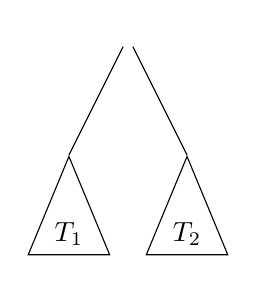
\begin{tikzpicture}
\usetikzlibrary{shapes.geometric}
\node {} [child anchor = apex]
child {node[draw, thin, isosceles triangle, anchor = apex, shape border rotate = 90]{$T_1$}}
child {node[draw, thin, isosceles triangle, anchor = apex, shape border rotate = 90]{$T_2$}};
\end{tikzpicture}

  \caption{Constructing a tree from subtrees}
  \label{fig:BinTreeConstruction}
\end{figure}

In addition to drawing pictures of binary trees, we can use a linear notation (something that can we written 
in the midst of prose). 
If $T_1$ and $T_2$ are simple binary trees, we may denote the tree constructed by grafting $T_1$ on the left and $T_2$ on the right
as $(T_1\curlywedge T_2)$ (as in Figure \ref{fig:BinTreeConstruction}. Thus we define simple binary trees, and two operations
on them, as follows.

\begin{defn}
\emph{Simple binary trees} are defined inductively by
\[T \defeq \bullet \,\mid\, (T_1\curlywedge T_2)\]
\end{defn}

The \emph{size} of a simple binary tree is a natural number defined by the equations
\begin{align*}
  \sz(\bullet) &\defeq 0\\
  \sz(T_1\curlywedge T_2) &\defeq 1 + \sz(T_1) + \sz(T_2)
\end{align*}
The \emph{height} of a simply binary tree a natural number is defined
by the equations
\begin{align*}
  \hght(\bullet) &\defeq 0\\
  \hght(T_1\curlywedge T_2) &\defeq 1 + \max(\hght(T_1),\hght(T_2))
\end{align*}
where $\max(m,n)$ is the larger of the two numbers.

These definitions suggest a relation between the size and height of a tree.
\ipadbreak

\begin{lemma}
For any simple binary tree $T$,  \[\hght(T)\leq \sz(T) < 2^{\hght(T)}.\]

\begin{proof}
To prove this by \emph{structural induction}, we must prove it for the basis ($\bullet$)
and that if it is true for some $T_1$ and $T_2$, then it is true for $(T_1\wedge T_2)$.
\begin{itemize}
\item{}[Basis] $\hght(\bullet) = 0$, $\sz(\bullet) = 0$ 
and $2^{\hght(\bullet)} = 1$. So the claim is true for $\bullet$.
\item{}[Inductive Hypothesis] Suppose the inequalities holds for some $T_1$ and $T_2$.
\item{}[Inductive Step] We must prove the two inequalities for $T= (T_1\curlywedge T_2)$.
Without loss of generality, assume that $\hght(T_1)\leq \hght(T_2)$. That is, if 
this is not so, then we may swap $T_1$ for $T_2$ in the following. 
\begin{align*}
\hght(T) &= 1 + \max(\hght(T_1),\hght(T_2)) &&\text{[Definition of $\hght$]}\\
         &\leq 1 + \hght(T_1) + \hght(T_2)  &&\text{[Arithmetic]}\\
         &\leq  1 + \sz(T_1) + \sz(T_2) &&\text{[Inductive Hypothesis]}\\
         &= \sz(T) &&\text{[Definition of $\sz$]}
       \end{align*}
And
\begin{align*}
\sz(T) &= 1 +\sz(T_1) + \sz(T_2)&&\text{[Definition of $\sz$]}\\
       &\leq 1 + 2^{\hght(T_1)} - 1) + (2^{\hght(T_2)} - 1)&&\text{[Inductive Hypothesis]}\\
       &\leq 2\cdot 2^{\hght(T_2)} - 1&&\text{[Assumption that $\hght(T_1)\leq \hght(T_2)$]}\\
       &= 2^{\hght(T_2)+1} - 1 &&\text{[Arithmetic]}\\
       &= 2^{\hght(T)} - 1 &&\text{[Definition of $\hght$]}
     \end{align*}
So $\sz(T) < 2^{\hght(T)}$
   \end{itemize}
 \end{proof}  
\end{lemma}

\ipadbreak

\begin{exer}
	\begin{exercise}
  \item Calculate the height and size of the following simple binary trees.
    \begin{enumerate}
    \item $(\bullet\curlywedge\bullet)$
    \item $(\bullet\curlywedge (\bullet\curlywedge\bullet))$
    \item $((\bullet\curlywedge\bullet)\curlywedge(\bullet\curlywedge(\bullet\curlywedge\bullet)))$
    \item $((\bullet\curlywedge(\bullet\curlywedge\bullet))\wedge ((\bullet\curlywedge\bullet)\curlywedge(\bullet\curlywedge(\bullet\curlywedge\bullet))))$
    \end{enumerate}
   \item Draw diagrams (similar to those in Figure \ref{fig:BinTree}) for the following
   simple binary trees.
   \begin{enumerate}
   \item $((\bullet \curlywedge \bullet)\curlywedge(\bullet\curlywedge\bullet))$
   \item $(((\bullet\curlywedge\bullet)\curlywedge\bullet)\curlywedge ((\bullet\curlywedge\bullet)\curlywedge(\bullet\curlywedge(\bullet\curlywedge\bullet))))$
   \end{enumerate}
   \item For each of the following diagrams, write the expression using $\bullet$ and $\curlywedge$
    defining the same tree.
\begin{multicols}{2}
    \begin{enumerate}
    \item 
\begin{tikzpicture}
\node {}
child {node {$\bullet$}}
child {node  {}
       child {node {$\bullet$}}
       child {node {$\bullet$}}
      };
\end{tikzpicture}

 \item 

\begin{tikzpicture}
[level/.style={sibling distance = 2cm/#1, level distance = 1.5cm}]
\node {}
child {node  {}
       child {node {$\bullet$}}
       child {node {$\bullet$}}
      }
child {node  {}
       child {node {$\bullet$}}
       child {node {$\bullet$}}
      };
\end{tikzpicture}

\item

\begin{tikzpicture}
\node {}
child {node  {}
       child {node {} 
              child {node {$\bullet$}}
              child {node {$\bullet$}}}
       child {node {$\bullet$}}
      }
child {node  {$\bullet$}};
\end{tikzpicture}

    \end{enumerate}
  \end{multicols}
  \end{exercise}
\end{exer}

We will study binary trees in more depth later in the course.

%
%
%\begin{exercise}
%\newcommand{\unit}{\mathord{\textbf{u}}}
%\newcommand{\B}{\mathord{\textbf{B}}}
%\newcommand{\C}{\mathord{\textbf{C}}}
%\newcommand{\denotation}{\mathord{\textsf{val}}}
%
%A \emph{widget} is defined inductively by
%\[M \defeq \unit \mid M\B \,\mid\, M\C\]
%
%For two widgets $M$ and $N$, their
%\emph{merge} is a widget, denoted by $M\oplus N$, defined by
%\begin{align*}
%\unit \oplus \unit &\defeq \unit\B\\
%\unit \oplus N\B &\defeq N\C\\
%\unit \oplus N\C &\defeq (\unit \oplus N)\B\\ 
%M\B \oplus \unit &\defeq M\C\\
%M\B \oplus N\B &\defeq (M\oplus N)\B\\
%M\B \oplus N\C &\defeq (M\oplus N)\C\\
%M\C \oplus \unit &\defeq  (M\oplus \unit)\B\\
%M\C \oplus N\B&\defeq (M\oplus N)\C\\
%M\C \oplus N\C&\defeq ((M\oplus N) \oplus \unit)\B
%\end{align*} 
%
%For a widget $M$, its \emph{value} is a natural number, denoted by
%$\llbracket M\rrbracket$, defined by
%\begin{align*}
%  \llbracket\unit\rrbracket &\defeq 1\\
%  \llbracket M\B\rrbracket &\defeq 2\cdot \llbracket M\rrbracket\\
%  \llbracket M\C\rrbracket &\defeq 2\cdot \llbracket M\rrbracket + 1
%\end{align*}
%
%Show that $\llbracket M\rrbracket + \llbracket N\rrbracket = \llbracket M\oplus N\rrbracket$ for any two
%widgets $M$ and $N$.
%\end{exercise}

%%% Local Variables: 
%%% mode: latex
%%% TeX-master: "MainText"
%%% End: 


\part{Basics of Sets and Functions}

\setTopic{Sets and Functions}
\setAuthor{M. Andrew Moshier}
\setDate{October 2014}
\setCourse{Discrete Mathematics}

\setOverview{
The mathematical universe consists of various things: numbers, functions, graphs, lists and so on.
A \noexpand\emph{set} is a collection of things. 
For example, the collection of all natural numbers is a set.
A \noexpand\emph{function} is a correlation of the members of one set with members of another set.
These two abstract concepts (sets and functions) form a conceptual framework in which virtually all of mathematics can be built.
So an understanding of sets and functions is key to a rigorous approach to most other parts of mathematics.
This conceptual framework can itself be put on a formal, precise footing called the Category of Sets and Functions.

In these lectures, we build up the Category of Sets and Functions, so that we can use these things as the basic building blocks of everything else we do.
}

\chapter{Sets}

\begin{goals}
\noindent\textbf{Lecture}
\begin{itemize}
\item Describe informally the category of sets.
\item Define list set notation.
\item Introduce the idea of a subset.
\item Introduce the axiom of extensionality for sets and some of its consequences.
\end{itemize}

\noindent\textbf{Study}
\begin{itemize}
\item Demonstrate ability to determine equality of sets.
\item Develop facility in basic set theoretic notation.
\end{itemize}
\end{goals}

\emph{Sets} are the mathematician's way of thinking about \emph{collections} of objects. Examples will be the set of natural numbers, the set of pairs of natural numbers, the set of lists of natural numbers, and so on.
\emph{Functions} are the mathematicians way of thinking about operations, such as successor, addition, summation, and so on.

Mathematicians also use functions to model attributes of the things in a collection, like ``the color of'', ``the mass of'', ``the location of'', ``the father of'', ``the favorite book of the person to the left of'' and so on.
There is little sense in saying these are ``operations'', but they have a similar behavior. For each potential
object $x$ of the right sort (a wooden building block, for example), \emph{the color of $x$} is a specific color. Similarly,
for a natural number $n$, ``the successor of $n$'' is another specific natural number. So ``the color of'' is a function
from the set of wooden building blocks to the set of colors; ``the successor of''
is a function from the set of natural numbers to set of natural numbers. Likewise, addition constitutes a function from the set of 
pairs of natural numbers to the set of natural numbers. In English we might say ``the sum of $m$ and $n$'', but we usually write $m+n$. 
Either way, any pair of natural numbers has a sum. So ``the sum of'' is an attribute of pairs of natural numbers, just like ``the color of'' is an attribute of wooden building blocks.

Taken together, sets and functions constitute a fundamental structure in contemporary mathematics called the \emph{Category of Sets and Functions}. 
This is a slight lie.
Actually, there are many different categories of sets that differ in subtle ways. 
But for most mathematics, the differences are irrelevant.
So in practice, it is safe to talk as if there is just one category of sets.
The Category of Sets and Functions sometimes abbreviated as \textbf{Set}.

To understand sets and functions as they are used in every day mathematics, we need to answer some questions:
\begin{itemize}
	\item What do we mean by saying that a set is a collection?
	\item What do we mean by saying that two sets are equal?
	\item What do we mean by saying that a function behaves like an attribute?
	\item What do we mean by saying that two functions are equal?
\end{itemize}
The answers to these leads to some basic principles for reasoning about sets and functions. 
Other principles allow us to construct sets and functions with specific behaviors. 
We could be more formal and present these principles as \emph{axioms}, but the word ``axiom''
has a special connotation in mathematics that we do not need here. Nevertheless, everything we say in these lectures could be presented in terms of formal axioms.  

\section{Set Basics}

A set consists of things that are ``in'' the set. All other things are ``not in'' the set. 
For example, later we will see that the natural numbers constitute a set $\NN$. 
So $0$ is in $\NN$, $1$ is in $\NN$, and so on, but $\frac{1}2$ is not in $\NN$.
We make this precise and introduce notation for the idea.

\begin{signature}\label{sig:SetSignature}
  A \emph{set} is a mathematical entity $A$ with the following feature. 
  For any thing $x$, either $x$ \emph{is in} $A$ or $x$ \emph{is not in} $A$. 
  We write $x\in A$ if $x$ is in $A$ and $x\notin A$ if $x$ is not in $A$.

The symbol $\in$ is used in mathematics exclusively to indicate membership in a set. 
You will not see it used in any other way.  

For variety, all of the following phrases mean the same thing:
\begin{itemize}
\item $x$ is in $A$
\item $x$ is an \emph{element of} $A$
\item $x$  is a \emph{member of} $A$
\item $A$ \emph{contains} $x$
\item $x$ \emph{belongs to} $A$
\end{itemize}
\end{signature}

Basic Vocabulary \ref{sig:SetSignature} describes how we can talk about sets and elements, and how to use the notation of membership, but does not tell us that any sets actually exist. 
We will remedy that in the next sections.
Our first remedy is to make room for finite sets.

\begin{principle}[Finite Sets] For any list $L  = [a_0,\ldots, a_{n-1}]$, there is a set, denoted by $\{a_0,\ldots,a_{n-1}\}$, so
  that $x\in \{a_0,\ldots, a_{n-1}\}$ if and only if $x=a_i$ for some
  $i<n$.  More precisely,
  \begin{itemize}
  \item $x\notin \{\}$ for any $x$ (so $\{\}$ is said to be \emph{empty});
  \item $x\in \{a_0,\ldots,a_n\}$ if and only if $x=a_0$ or $x\in
    \{a_1,\ldots,a_n\}$.
  \end{itemize}
\end{principle}

\printbreak

\begin{example}
Here are some examples of sets built from finite lists:
\begin{itemize}
\item $\{\}$ -- an empty set;
\item $\{1,2,5\}$ -- a set consisting of three elements;
\item $\{\{\}\}$ -- a set consisting of one element, which is $\{\}$;
\item $\{1,2,4,\{1,2\}\}$ -- a set consisting of four elements, $1$,
  $2$, $4$ and the set $\{1,2\}$.
\item $\{4,5, \{\}, [\,]\}$ -- a set consisting of four elements. Note that
the set $\{\}$ and the list $[\,]$ are not the same things.
\item $\{1,2,3,4,3,2,1\}$ -- a set consisting of four elements, listing an element twice is redundant.
\end{itemize}
\end{example}

The study of finite sets is surprisingly complex, and comprises a large part of
the branch of mathematics called \emph{combinatorics}. We will touch on some basics
of combinatorics later in the course. 

Various infinite sets of numbers also exist. All of these are indeed sets (that is, their existence follows from general principles
of set theory), but we will not try to justify that explicitly, except for the set of natural numbers.

\begin{defn}
	The following sets are denoted by special symbols:
	\begin{align*}
		\NN &= \text{the set of natural numbers}\\
		\ZZ &= \text{the set of integers}\\
		\QQ &= \text{the set of rational numbers}\\
		\RR &= \text{the set of real numbers}\\
		\CC &= \text{the set of complex numbers}
	\end{align*}
\end{defn}


\begin{exercises}
	\begin{enumerate}
  \item Let $A = \{1,\{2,3\},4\}$. Determine which of the following assertions are true.
    \begin{enumerate}
    \item $1\in A$
    \item $2\in A$
    \item $\{\}\in A$
    \item $\{2,3\}\in A$
    \item $A\in A$
    \end{enumerate}
  \item In the following examples of sets with elements following a pattern, write an expression for the same set
  that makes the pattern clearer.
  \begin{enumerate}
  \item $\{0,2,4,\ldots, 100\}$
  \item $\{1,2,4,8,\ldots, 256\}$
  \item $\{0,1,3, 6, 10,\ldots, 55\}$
  \end{enumerate}
  \end{enumerate}
\end{exercises}

\section{Subsets and Extensionality}

Sets are meant to be bare collections. For a set $A$, some things are in $A$, some are not. And that's all we can say.
Unlike a list, a set has no ``initial'' element.
For example, the set $\{1,2,3\}$ should be the same as the set $\{2,3,1\}$, because both have the same elements. This is an important difference between
lists and sets: $[1,2,3]$ and $[2,3,1]$ are \emph{not} the same lists because order matters in lists. 
To make this precise, we need to be clear about when sets are equal. To do this, we introduce an important definition.

\begin{defn}
  For sets $A$ and $B$, we say that \emph{$A$ is a subset of $B$} provided that every element of $A$ is an element of $B$. We also
  write this as $A\subseteq B$, and say that \emph{$A$ is included in $B$}.  We may also write $B\supseteq A$ 
  to mean the same thing, and say that \emph{$B$ is a superset of $A$}.

  If $A$ is \emph{not} a subset of $B$, we write $A\not\subseteq B$. If $A\subseteq B$ and $B\not\subseteq A$, then $A$ is called a
  \emph{proper subset of $B$}. To indicate that $A$ is a \emph{proper} subset of $B$, we may write $A\subsetneq B$.
\end{defn}

Saying $A\subseteq B$ is exactly the same as saying that for any $x$, if $x\in A$ then $x\in B$.

\begin{example}
  Here are some examples and counter-examples of the subset relation.
  \begin{itemize}
  \item $\{1,2,3\}\subseteq \{0,1,2,3\}$
  \item $\{\}\subseteq \{0\}$
  \item $A\subseteq A$ for any set $A$ because, trivially, every
    element of $A$ is an element of $A$
  \item $\{\} \subseteq A$ for any set $A$ because every element of
    $\{\}$ (there are none) is an element of $A$
  \item $\{1,2,3\}\not\subseteq \{0,2,3\}$ because $1\in \{1,2,3\}$
    but $1\notin \{0,2,3\}$
  \item $\{1,2,3\}\subseteq \{2,3,1\}$
  \end{itemize}
\end{example}

\ipadbreak

\begin{exercises}
	For each of the following pairs of sets, determine whether or
  not the first is a subset of the second. Explain your answer.
  \begin{enumerate}[series=exercises]
  \item $\{0,1\}$ and $\{1,0\}$
  \item $\{a,b,c,d\}$ and $\{a,b,d,e,c\}$
  \item $\{\}$ and $\{\{\}\}$
  \item $\{0,3,6,10\}$ and $\{10,9,8,7,6,5,4,2,1, 0\}$
  \end{enumerate}
\end{exercises}


We can summarize two useful properties of $\subseteq$ as follows.
\begin{itemize}
	\item{}[Reflexivity]  For any set $A$, $A \subseteq A$. We say $\subseteq$ is \emph{reflexive}.
	\item{}[Transitivity] For any sets $A$, $B$ and $C$,
	if $A\subseteq B$ and $B\subseteq C$, then $A\subseteq C$. We say $\subseteq$ is \emph{transitive}.
\end{itemize}
Another familiar example of a reflexive, transitive
relation is $\leq$ on the natural numbers. In fact there are many examples of reflexive transitive relations throughout mathematics. 

The relation $\leq$ is also \emph{anti-symmetric}, meaning that if $m\leq n$ and $n\leq m$ then $m=n$. 
Suppose $A\subseteq B$ and $B\subseteq A$. Then, by definition $A$ and $B$ have the exact same elements.  By our understanding of sets as collections,
$A$ and $B$ must be equal. So we state this as another axiom.

\begin{principle}\label{ax:set-extensionality}
[\textbf{The Axiom of Set Extensionality}]
For sets $A$ and $B$, if $A\subseteq B$ and $B\subseteq A$, then $A=B$. In other words, $\subseteq$ is anti-symmetric.
\end{principle}

Based on this, we can already establish a useful fact: there is exactly one empty set. To set the tone for what follows, we make this a formal claim.

\begin{lemma}
	There is exactly one empty set.
\begin{proof}
	We have already noted that the set built from an empty list $\{\,\}$ has no elements. So there is at least one empty set.
	
	Suppose $E$ is a set with no elements.
	Then $E\subseteq \{\,\}$ because every element of $E$ (there are none) is an element of $\{\,\}$. 
	Similarly, $\{\,\}\subseteq E$ because every element of $\{\,\}$ (again, there are none) is an element of $E$. 
	So by Principle~\ref{ax:set-extensionality} $E = \{\,\}$.
\end{proof}
\end{lemma}

\begin{defn}
  The set $\{\}$ is also denoted by $\emptyset$.
\end{defn}

Set extensionality makes precise the idea that a set by itself does
not have any structure other than what members it possesses.
To emphasize this, sometimes it is useful to
depict a set with elements scattered about something like \usetikzlibrary{fit,shapes}
\[\begin{tikzpicture}[ >=stealth, bullet/.style={ fill=black, circle,
    minimum width=1pt, inner sep=2pt }, projection/.style={ ->, thick,
    shorten <=2pt, shorten >=2pt }, every fit/.style={ ellipse, draw,
    inner sep=2pt } ]
  \foreach \x/\y/\l in {0.4/1/d,-0.2/2/c/,0/3/b,0.5/4/a}
  \node[bullet,label=left:$\l$] (a\y) at (\y,\x) {};
  \node[draw,fit=(a1) (a2) (a3) (a4),minimum width=2cm] {} ;
\end{tikzpicture}
\]
with the elements scattered about. Evidently, a re-arrangement of the
elements does not change the depicted set. So
\[\usetikzlibrary{fit,shapes}
\begin{tikzpicture}[ >=stealth, bullet/.style={ fill=black, circle,
    minimum width=1pt, inner sep=2pt }, projection/.style={ ->, thick,
    shorten <=2pt, shorten >=2pt }, every fit/.style={ ellipse, draw,
    inner sep=2pt } ]
  \foreach \x/\y/\l in {0.3/2/d,-0.2/3/c/,0/4/b,-0.5/1/a}
  \node[bullet,label=left:$\l$] (a\y) at (\y,\x) {};
  \node[draw,fit=(a1) (a2) (a3) (a4),minimum width=2cm] {} ;

\end{tikzpicture}
\]
is the same set. Depicting a subset of a set is a simple
matter of drawing a smaller boundary around some of the elements as in the following.
\[\usetikzlibrary{fit,shapes}
\begin{tikzpicture}[ >=stealth, bullet/.style={ fill=black, circle,
    minimum width=1pt, inner sep=2pt }, projection/.style={ ->, thick,
    shorten <=2pt, shorten >=2pt }, every fit/.style={ ellipse, draw,
    inner sep=2pt } ]
  \foreach \x/\y/\l in {0.3/2/d,-0.2/3/c/,0/4/b,-0.5/1/a}
  \node[bullet,label=left:$\l$] (a\y) at (\y,\x) {};
  \node[draw,fit=(a1) (a2) (a3) (a4),minimum width=2cm] {} ;
  \node[draw, fit = (a2) (a3), minimum width=2cm] {};
\end{tikzpicture}
\]
\ipadbreak

\begin{exercises}
Draw depictions of the following sets
  \begin{enumerate}[resume=exercises]
  \item $\{1,4,5,2,3\}$
  \item $\{1,2,3,\ldots, 23\}$
  \item $\{a,b,c,d,e\}$ and $\{c,e,f,g\}$ on the same diagram
  \item $\{a, e, b,c,e\}$ [sic]
  \item $\{1,3,6,7\}$ and $\{1,3,5,6,7,9\}$ on the same diagram
  \item $\{\bot,\top$
  \item $\{\bullet\}$
  \item $\{\top,\bot,3,5,1, \bullet\}$
  \end{enumerate}
\end{exercises}

\chapter{Functions}

\begin{goals}
\noindent\textbf{Lecture}
\begin{itemize}
\item Introduce basic structure of functions
\item Define the identity functions and function composition
\item Introduce internal diagrams of functions.
\end{itemize}

\noindent\textbf{Study}
\begin{itemize}
\item Be able to determine equality of functions
\item Use internal diagrams to depict function composition
\end{itemize}
\end{goals}

\emph{Functions} (perhaps in your calculus courses) are often talked about as \emph{operations}. 
For example, 
\[f(x) = x^2-1\]
can be seen as an operation that transforms a number $x$ into its square.
But it can also be seen as an attribute (the ``square of $x$'').
The ``operational'' view is informal, and often useful.
As we will see, though, it gets an important aspect of functions wrong because two entirely different operations may define the same function.

Informally, a function ``takes'' an argument from a given set as input and ``produces'' an output in a given set.
So the function $f$ defined by $f(x)=x^2 + 2x + 1$ might ``take'' the natural number $2$ and ``produce'' the natural number $10$. 
That is, $f(3)=3^2 + 1 = 10$. 
We begin by introducing the vocabulary of functions.

\begin{signature}
	\begin{itemize}
	\item For a set $A$ and a set $B$, there are things called \emph{functions from $A$ to $B$}, with a function $f$ from $A$ to $B$ being writing $\fromto fAB$ or $A\stackrel{f}{\to} B$. 

	\item For $\fromto fAB$, the set $A$ is called the \emph{domain} of $f$ and $B$ is called the \emph{codomain} of $f$.
	
	\item For any function $\fromto fAB$ and every element $a\in A$, $f$ and $a$ determine an element of $B$, written $f(a)$, and read ``$f$ of $a$''.
	\end{itemize}
\end{signature}

A functions may sometimes also be called a \emph{map}, a \emph{transformation}, or an \emph{operation}. 
As we will see, however, \emph{operation} is somewhat misleading. 

Often, a function $\fromto fAB$ is \emph{defined} by a rule, just as they are familiar in other parts of mathematics. 
We typically, write such rules by giving the function a name (very often $f$) and spelling out the rule at the same time.
So we write things like
\[f(x)=x^2 + 4x + 2\]
to define a function $\fromto f\RR\RR$ (recall that $\RR$ is the set of real numbers).
But sometimes it is useful to have a rule without giving it a name.
To do that, we use the ``maps to'' arrow $\mapsto$.
So we might define the same function $f$ by saying that \emph{$f$ is given by the rule $x\mapsto x^2 + 4x + 2$}. 
We will not go so far as to write $f = (x\mapsto x^2+4x+2)$ because this more easily understood by writing $f(x)=x^2+4x+2$.
The rule $x\mapsto x^2  4x + 2$ is the same as the rule $y\mapsto y^2 + 4y + 2$. 
The variable only serves as a place holder, so its particular name does not matter.

There are two fundamental (trivial) types of rules that can be used to build functions.

\begin{axiom}
	\begin{itemize}
		\item For any set $A$, there is a function $\fromto {\id_A}AA$ defined by the rule $x\mapsto x$.
		This is called the \emph{identity} function on $A$
		\item For any two functions $\fromto fAB$ and $\fromto gBC$, there is a function $\fromto {g\circ f}AC$ defined by the rule $x\mapsto g(f(x))$.
		This is called the composition of $g$ and $f$ (or sometimes ``$g$ following $f$'').
	\end{itemize}
\end{axiom}

Notice that $g\circ f$ is only defined when the \emph{domain} of $g$ matches the codomain of $f$.
Also, be careful about definitions like $f(x)=1/x$.
This does not define a function on the real numbers because $f(0)$ is undefined.
In other words, to be a function, $f$ must determine an element of the codomain for each element of the domain.

\begin{exercises}
Suppose $\fromto fAB$, $\fromto gBC$ and $\fromto hCD$ are functions. Then $h\circ(g\circ f)$ and $(h\circ g)\circ f$ are functions
from $A$ to $D$. Do you think they are equal? Explain your answer in a few clearly written sentences.	
\end{exercises}

\section{Internal Diagrams}

To depict a function on small sets, we can use the simple internal diagrams of the last section. For example,
\[
  \begin{tikzpicture}[
    >=stealth,
    bullet/.style={
      fill=black,
      circle,
      minimum width=1pt,
      inner sep=1pt
    },
    projection/.style={
      ->,
      thick,
      shorten <=2pt,
      shorten >=2pt
    },
    every fit/.style={
      ellipse,
      draw,
      inner sep=0pt
    }
  ]
    \foreach \x/\y/\l in {0.4/1/d,-0.2/2/c/,0/3/b,0.5/4/a}
      \node[bullet,label=left:$\l$] (a\y) at (\x,\y) {};

    \foreach \x/\y/\l in {4.1/1/4,3.2/2/3,4.3/3/2,4/4/1}
      \node[bullet,label=right:$\l$] (b\y) at (\x,\y) {};

    \node[draw,fit=(a1) (a2) (a3) (a4),minimum width=2cm] {} ;
    \node[draw,fit=(b1) (b2) (b3) (b4),minimum width=2cm] {} ;

    \draw[projection] (a1) -- (b4);
    \draw[projection] (a2) -- (b2);
    \draw[projection] (a3) -- (b1);
    \draw[projection] (a4) -- (b3);
  \end{tikzpicture}
\]
depicts a function from the set $\{a,b,c,d\}$ to the set $\{1,2,3,4\}$.

Composition can be illustrated using internal diagrams.
For example,
  \[
    \begin{tikzpicture}[
      >=stealth,
      bullet/.style={
        fill=black,
        circle,
        minimum width=1pt,
        inner sep=1pt
      },
      projection/.style={
        ->,
        thick,
        shorten <=2pt,
        shorten >=2pt
      },
      projectionC/.style={
        ->,
        thick,
        dashed,
        shorten <=2pt,
        shorten >=2pt
      },
      every fit/.style={
        ellipse,
        draw,
        inner sep=0pt
      }
    ]
      \foreach \x/\y/\l in {0.4/1/d,-0.2/2/c/,0/3/b,0.5/4/a}
        \node[bullet,label=left:$\l$] (a\y) at (\x,\y) {};

      \foreach \x/\y/\l in {3.5/2/4,4.1/3/3,3.2/4/2,4/5/1}
        \node[bullet,label=below:$\l$] (b\y) at (\x,\y) {};

      \foreach \x/\y/\l in {7.8/1/u,8.2/2/v,7.3/3/w,7.9/4/x, 8.0/5/z}
        \node[bullet,label=right:$\l$] (c\y) at (\x,\y) {};

      \node[blue] at (2,5) {$f$};
      \node[green] at (6,5.5) {$g$};
      \node[red] at (4,0.5) {$g\circ f$};

      \node[draw,fit=(a1) (a2) (a3) (a4),minimum width=2cm] {} ;
      \node[draw,fit=(b2) (b3) (b4) (b5),minimum width=2cm] {} ;
      \node[draw,fit=(c1) (c2) (c3) (c5),minimum width=2cm] {} ;

      \draw[projection,blue] (a1) -- (b2);
      \draw[projection,blue] (a2) -- (b2);
      \draw[projection,blue] (a3) -- (b3);
      \draw[projection,blue] (a4) -- (b5);
      \draw[projection,green] (b2) -- (c1);
      \draw[projection,green] (b3) -- (c2);
      \draw[projection,green] (b4) -- (c3);
      \draw[projection,green] (b5) -- (c5);
      \draw[projectionC,red] (a1) -- (c1);
      \draw[projectionC,red] (a2) -- (c1);
      \draw[projectionC,red] (a3) -- (c2);
      \draw[projectionC,red] (a4) -- (c5);
    \end{tikzpicture}
	\]
	
\begin{exercises}
	Use internal diagrams for the following exercises.
	\begin{enumerate}
		\item Depict four different functions from the set $\{1,2,3\}$ to the set $\{\bot,\top\}$. [Draw four different diagrams.]
		\item Depict all of the functions from $\{\bullet\}$ to $\{a,b,c\}$
		\item Depict all of the functions from $\{a,b,c\}$ to $\{\bullet\}$
		\item Are there any functions from $\{a,b\}$ to $\emptyset$?
		\item Are there any functions from $\emptyset$ to $\{a,b\}$? If there are, how many?
		\item For each of the following diagrams, determine whether or not the
  diagram depicts a function. If not, explain why not.
  \begin{multicols}{2}
    \begin{enumerate}
    \item
      \begin{tikzpicture}[ scale=.75, >=stealth, bullet/.style={
          fill=black, circle, minimum width=1pt, inner sep=1pt },
        projection/.style={ ->, thick, shorten <=2pt, shorten >=2pt },
        every fit/.style={ ellipse, draw, inner sep=0pt } ]
        \foreach \x/\y/\l in {0.4/1/d,-0.2/2/c/,0/3/b,0.5/4/a}
        \node[bullet,label=left:$\l$] (a\y) at (\x,\y) {};

        \foreach \x/\y/\l in {4.1/1/4,3.2/2/3,4.3/3/2,4/4/1}
        \node[bullet,label=right:$\l$] (b\y) at (\x,\y) {};

        \node[draw,fit=(a1) (a2) (a3) (a4),minimum width=2cm] {} ;
        \node[draw,fit=(b1) (b2) (b3) (b4),minimum width=2cm] {} ;

        \draw[projection] (a1) -- (b4); \draw[projection] (a2) --
        (b3); \draw[projection] (a3) -- (b1); \draw[projection] (a4)
        -- (b3);
      \end{tikzpicture}
    \item \begin{tikzpicture}[ scale=.75, >=stealth, bullet/.style={
          fill=black, circle, minimum width=1pt, inner sep=1pt },
        projection/.style={ ->, thick, shorten <=2pt, shorten >=2pt },
        every fit/.style={ ellipse, draw, inner sep=0pt } ] \foreach
        \x/\y/\l in {0.4/1/d,-0.2/2/c/,0/3/b,0.5/4/a}
        \node[bullet,label=left:$\l$] (a\y) at (\x,\y) {};

        \foreach \x/\y/\l in {4.1/1/4,3.2/2/3,4.3/3/2,4/4/1}
        \node[bullet,label=right:$\l$] (b\y) at (\x,\y) {};

        \node[draw,fit=(a1) (a2) (a3) (a4),minimum width=2cm] {} ;
        \node[draw,fit=(b1) (b2) (b3) (b4),minimum width=2cm] {} ;

        \draw[projection] (a1) -- (b4); \draw[projection] (a2) --
        (b3); \draw[projection] (a3) -- (b1); \draw[projection] (a4)
        -- (b3); \draw[projection] (a2) -- (b2);
      \end{tikzpicture}
    \item \begin{tikzpicture}[ scale=.75, >=stealth, bullet/.style={
          fill=black, circle, minimum width=1pt, inner sep=1pt },
        projection/.style={ ->, thick, shorten <=2pt, shorten >=2pt },
        every fit/.style={ ellipse, draw, inner sep=0pt } ] \foreach
        \x/\y/\l in {0.4/1/d,-0.2/2/c/,0/3/b,0.5/4/a}
        \node[bullet,label=left:$\l$] (a\y) at (\x,\y) {};

        \foreach \x/\y/\l in {4.1/1/4,3.2/2/3,4.3/3/2,4/4/1}
        \node[bullet,label=right:$\l$] (b\y) at (\x,\y) {};

        \node[draw,fit=(a1) (a2) (a3) (a4),minimum width=2cm] {} ;
        \node[draw,fit=(b1) (b2) (b3) (b4),minimum width=2cm] {} ;

        \draw[projection] (a1) -- (b1); \draw[projection] (a2) --
        (b1); \draw[projection] (a3) -- (b1); \draw[projection] (a4)
        -- (b1);
      \end{tikzpicture}
    \item \begin{tikzpicture}[ scale=.75, >=stealth, bullet/.style={
          fill=black, circle, minimum width=1pt, inner sep=1pt },
        projection/.style={ ->, thick, shorten <=2pt, shorten >=2pt },
        every fit/.style={ ellipse, draw, inner sep=0pt } ] \foreach
        \x/\y/\l in {0.4/1/d,-0.2/2/c/,0/3/b,0.5/4/a}
        \node[bullet,label=left:$\l$] (a\y) at (\x,\y) {};

        \foreach \x/\y/\l in {4.1/1/4,3.2/2/3,4.3/3/2,4/4/1}
        \node[bullet,label=right:$\l$] (b\y) at (\x,\y) {};

        \node[draw,fit=(a1) (a2) (a3) (a4),minimum width=2cm] {} ;
        \node[draw,fit=(b1) (b2) (b3) (b4),minimum width=2cm] {} ;

        % \draw[projection] (a1) -- (b4);
        \draw[projection] (a2) -- (b3); \draw[projection] (a3) --
        (b1); \draw[projection] (a4) -- (b3);
      \end{tikzpicture}
	  \end{enumerate}
	  \end{multicols}
		\item Let $A = \{1,2,3\}$. Let $B=\{a,b,c,e\}$ and let $C = \{\bot,\top\}$.
		Depict some functions $\fromto fAB$, $\fromto gBC$, and $g\circ f$. 
		\item Think about how you might depict a function $\fromto hAA$ using only one picture of the set $A$.
		Describe what you would do, and provide an example.
		\item Suppose $\fromto f\RR\RR$ is given by the rule $x\mapsto x^2$, suppose $\fromto g\RR\RR$ is given
		by the rule $x\mapsto x-1$. Write rules for $f\circ g$ and $g\circ f$ without using the symbols $f$ and $g$. Explain whether or not it is the case that $f\circ g = g\circ f$.
	\end{enumerate}
\end{exercises}

\section{Extensionality}

Just like sets, we need a way to say when two functions are equal.
Let $\NN$ denote the set of natural numbers. 
Then define $\fromto f\NN\NN$ by
\[f(n) = n^2 +  2n + 1.\]
Likewise, define $\fromto g\NN\NN$ by
\[g(n) = (n+1)^2.\]
Evidently, for each $n\in\NN$, it is true that $f(n) = g(n)$.
So even though $f$ and $g$ are defined by different \emph{operations}, the two functions yield the same results.
As with sets, this leads to an axiom for equality of functions.

\begin{axiom}[\textbf{The Axiom of Function Extensionality}]
	For functions $\fromto fAB$ and $\fromto gAB$, if it is the case that $f(x)=g(x)$ for all $x\in A$, then $f=g$.
	Note that equality of functions only makes sense when the two functions share the same domain and the same codomain.
\end{axiom}

If we not concerned about the detailed internals sets, but only with how functions interact, then function can be depicted very simply as $A\stackrel{f}{\longrightarrow} B$.
So a composition of functions can be depicted as in
\[
\tikzset{>=stealth}
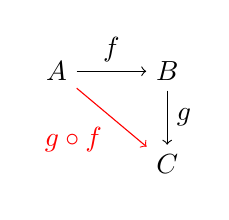
\begin{tikzpicture}[every node/.style={midway}]
\matrix[column sep={4em,between origins},
        row sep={2em}] at (0,0)
{ \node(A)   {$A$}  ; & \node(B) {$B$}; \\
                      & \node(C) {$C$}; \\};
\draw[->] (A) -- (B) node[anchor=south]  {$f$};
\draw[->] (B) -- (C) node[anchor=west]  {$g$};
\draw[->,red] (A) -- (C) node[anchor=north east] {$g\circ f$};
\end{tikzpicture}
\]
We do not really need to draw $g\circ f$ as a separate arrow because the \emph{path} from $A$ to $B$ to $C$ is already implicitly a depiction of $g\circ f$.
So the simpler diagram 
\[
\tikzset{>=stealth}
\begin{tikzpicture}[every node/.style={midway}]
\matrix[column sep={4em,between origins},
        row sep={2em}] at (0,0)
{ \node(A)   {$A$}  ; & \node(B) {$B$}; \\
                      & \node(C) {$C$}; \\};
\draw[->] (A) -- (B) node[anchor=south]  {$f$};
\draw[->] (B) -- (C) node[anchor=west]  {$g$};
\end{tikzpicture}
\]
shows the same information, namely, that $\fromto fAB$ and $\fromto gBC$ are functions and therefore, $g\circ f$ is too.

Now a diagram such as this
\[
\tikzset{>=stealth}
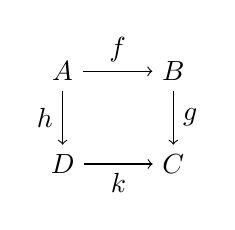
\begin{tikzpicture}[every node/.style={midway}]
\matrix[column sep={4em,between origins},
        row sep={2em}] at (0,0)
{ \node(A)   {$A$}  ; & \node(B) {$B$}; \\
  \node(D)   {$D$}  ; & \node(C) {$C$}; \\};
\draw[->] (A) -- (B) node[anchor=south]  {$f$};
\draw[->] (B) -- (C) node[anchor=west]  {$g$};
\draw[->] (A) -- (D) node[anchor=east] {$h$};
\draw[->] (D) -- (C) node[anchor=north] {$k$};
\end{tikzpicture}
\]
depicts two composite functions $g\circ f$ and $k\circ h$, but $g\circ f$ and $k\circ k$ may not be equal.
We say that the diagram \emph{commutes} or that it is a \emph{commutative diagram} if $g\circ f = k\circ h$.
In other words, saying that a certain diagram commutes \emph{is} an assertion that certain functions are equal.


\begin{exercises}
\begin{enumerate}
\item  For each of the following pairs of functions $\NN\to\NN$, determine whether they are equal and explain why or why not.
  \begin{enumerate}
  \item $f(n) = 2n + 3$ and $g(m) = 2m + 3$
  \item $f(n) = 2^{n+1} - 1$ and $g(n) = \sum_{i=0}^n2^i$
  \item $f(n) =  n^2 + 5n + 6$ and $g(n) = (n+3)(n+2)$
  \item $f(n) = n^4 - 10n^3 + 35n^2 + 50n + 24$ and $g(n) = 24$
  \end{enumerate}
\item Let $\RR$ denote the set of all real numbers. Let $f(x) = \tan(x)$.
Explain why this does \emph{not} define a function from $\RR$ to $\RR$.
\item Suppose the following functions exist: $\fromto fAB$, $\fromto gBC$, $\fromto aAD$, $\fromto bCD$. 
  Draw a commutative diagram asserting that $b\circ g\circ f = a$.
\item Suppose the following functions exist: $\fromto fCA$, $\fromto gCB$, $\fromto hCP$, $\fromto pPA$ and $\fromto qPB$.
 Draw a commutative diagram asserting that $f=p\circ h$ and $g=q\circ h$.
\end{enumerate}
\end{exercises}

\chapter{Basic Building Blocks}

\begin{goals}
	\noindent\textbf{Lecture}
	\begin{itemize}
	\item Characterize and define
		 \begin{itemize}
			 \item Pointer and constant functions
			\item Solution sets
			\item Characteristic functions
			%		 	\item The set of natural numbers
			\item Products of sets
			\item Exponents of sets
		 \end{itemize}
	\item Introduce the idea of a \emph{universal} construction.
	\end{itemize}

	\noindent\textbf{Study}
	\begin{itemize}
	\item Be able to calculate membership in various constructed sets 
	\item Learn to use universal constructions to define functions. 
	\end{itemize}
\end{goals}

So far, we have been able to think mainly about finite sets and a few informally defined functions on, say, the real numbers or the natural numbers.
To fill out our understanding of sets, we need to be able to build sets for specific purposes.

Two finite sets will play particularly important roles.
The first, which we denote by $\One$, is  set with one element; the second, which we denote by $\Two$, is a set with two elements.
It does not matter at all \emph{what} elements are in these because, as we will soon see, any two sets of the same size are interchangeable.
What `interchangeable' means is discussed later.
What `same size' means is obvious for finite sets, but not at all apparent for infinite ones.
We discuss the general situation later as well.

For the time being, we merely need to agree on a fixed set with one element and a fixed set with two elements.
The particular choices I make here will be clearer as we put them to use.

\begin{defn}
	Let $\bullet$, $\bot$ and $\top$ be fixed symbols. Then define
	\begin{align*}
		\One &= \{\bullet\}\\
		\Two &= \{\bot,\top\}
	\end{align*} 
	The single element of $\One$ is intended to look like a generic point in an internal diagram.
	The element $\top$ is meant to remind you of the letter `T' (short for `True') and $\bot$ is meant to be the opposite of $\top$ (that is, 'False').
\end{defn}


\section{Elements, Pointers and Constant Functions}

Suppose we are told that $\fromto p\One A$ is a function.
Since $\bullet\in\One$, this function determines an element of $A$, namely $p(\bullet)$.
A picture of the situation might be this:
\[
  \begin{tikzpicture}[
    >=stealth,
    bullet/.style={
      fill=black,
      circle,
      minimum width=1pt,
      inner sep=1pt
    },
    projection/.style={
      ->,
      thick,
      shorten <=2pt,
      shorten >=2pt
    },
    every fit/.style={
      ellipse,
      draw,
      inner sep=0pt
    }
  ]
    \node[bullet] (p) at (0,2.5) {};

    \foreach \x/\y/\l in {4.1/1/4,3.2/2/3,4.3/3/2,4/4/1}
      \node[bullet,label=right:$\l$] (a\y) at (\x,\y) {};

    \node[draw,fit=(p),minimum width=1cm, minimum height=1cm] {} ;
    \node[draw,fit=(a1) (a2) (a3) (a4),minimum width=2cm] {} ;

    \draw[projection] (p) -- (a3);
  \end{tikzpicture}
\]
Since $\One$ has only a single element, it can ``point'' only to a single element of $A$.
So we might refer to a function $\One\to A$ as a \emph{pointer} into $A$.
Each pointer determines an element of $A$. 
And conversely, it should be possible to point to any element of $A$. 
This leads to our first axiom guaranteeing that certain functions exist.

\begin{principle}\label{ax:pointers}
	For any set $A$, and any $a\in A$, there is a pointer $\fromto {\hat a}\One A$ so that $\hat{a}(\bullet)=a$.
\end{principle}

In effect, this principle claims that elements of a set $A$ and functions $\One\to A$ are interchangible: from $a\in A$ we get $\fromto {\hat{a}}\One A$; from $\fromto p\One A$.
we get $p(\bullet)$. 

This principle also justifies the drawing of internal diagrams for pointers because it means that any such diagram does depict an actual function. 
Other principles that we will discuss later justify our use of internal diagrams for all finite sets.

We can specify $\hat{a}$ by the rule $x\mapsto a$.
That is, since $\bullet$ is an element of $\One$, $\hat{a}(\bullet)=a$.
And since $\bullet$ is the only element of $\One$, $\hat{a}{x}=a$ is true for \emph{every} element of $\One$.

Suppose $\fromto fA\One$ and $\fromto gA\One$ are functions, that is, their \emph{codomain} is $\One$ instead their \emph{domain}. 
Then $f(a)=g(a)$ is true for every $a\in A$ because $\bullet$ is the only possible value for $f(a)$ and $g(a)$. 
So $f=g$ by the Principle of Function Extensionality.
In other words, there is at most one function from $A$ to $\One$.
But the rule $x\mapsto \bullet$ is as simple a rule as one can imagine. 
This leads to another axiom.

\begin{defn}\label{def:terminal}
	A set $T$ is \emph{terminal} if it is the case that for any set $A$ there is exactly one function from $A$ to $T$.
\end{defn}

\begin{axiom}
	The set $\One$ is a terminal set. 
	We denote the unique function from $A$ to $\One$ by $\fromto {\Diamond_A}{A}\One$.
	
	The rule defining $\Diamond_A$ must be
	\[x\mapsto\bullet\]
	because no other rule is possible. 
\end{axiom}

Using $\Diamond_A$ and $\hat{b}$ for an element $b\in B$, we can now define constant functions. 
That is $\hat{b}\circ\Diamond_A$ is a function from $A$ to $B$ defined by 
\[(\hat{b}\circ\Diamond_A)(x) = \hat{b}(\Diamond_A(x))= \hat{b}(\bullet) = b.\] 
In short, this is the function sending any element of $A$ to the constant result $b$. 

\begin{exercises}
	\begin{enumerate}
		\item Show that for any pointer $\fromto p\One A$, it is the case that $\widehat{p(\bullet)}=p$.
		\item Show that any set with exactly one element is a terminal set.
		\item Suppose that $\fromto fAB$ is a function. Show that for every $a\in A$, $\widehat{f(a)} = f\circ \hat{a}$.
	\end{enumerate}
\end{exercises}

\section{Solution Sets, Subsets, Characteristic Functions}

Suppose we are given two functions that are ``parallel'': $\fromto fAB$ and $\fromto gAB$.
Then for some value $a\in A$, it might be the case that $f(a)=g(a)$.
We may call such a value a \emph{particular solution to the equation $f(x)=g(x)$}. 
It might be the case that there are no particular solutions.
For example, there are no natural numbers $n$ such that $n+1 = n$. 
On the other hand, there might be many particular solutions. 
For example, let $f(x)=x^3$ and let $g(x)= 6x^2 - 11x + 6$ both as functions on the natural numbers.
Then it is easy to check that $1$, $2$ and $3$ solve the equation.
In fact, these three are the only particular solutions.
We generalize as follows.

\begin{defn}\label{def:equalizer} 
	For two functions $A\doublerightarrow{f}{g} B$, a \emph{solution} is a function $\fromto sCA$ so that 
	\[f\circ s = g\circ s.\]
	Thus for example, if $a\in A$ is a particular solution then the pointer $\hat a$ is a solution. 

	For functions $\fromto fAB$ and $\fromto gAB$, an \emph{equalizer} is solution $\fromto eEA$ so that for any solution $\fromto sCA$, there is exactly one function $\fromto hCE$ so that \[e\circ h = k.\]
\end{defn}

\begin{principle}
	For functions $A\doublerightarrow{f}{g} B$, the collection of all particular solutions to the equation $f(x)=g(x)$ form a set, denoted by $\{x\in A\st f(x) = g(x)\}$. 	
	The function $\fromto i{\{x\in A\st f(x)=g(x)\}}A$ given by the rule $x\mapsto x$ (called an \emph{inclusion map}) is an equalizer for $f$ and $g$.
	
	If $\fromto sCA$ is a solution of  $f(x)=g(x)$, that is, $f\circ s = g\circ s$,
	then the function $\fromto {\check s}C{\{x\in A\st f(x)=g(x)\}}$ given by the rule $x\mapsto s(x)$
	is the unique function for which $s = i\circ \check s$. 
\end{principle}

This axiom tells us three main things.
First, we can form a subset of $A$ by specifying an equation $f(x)=g(x)$ for any two functions $A\doublerightarrow{f}{g}B$, and picking out the particular solutions.
Second, a subset formed in this way ``embeds'' in the given set $A$ by its inclusion map $i$.
Third, for any solution $s$, the function into the set of particular solutions is defined by the same rule as $s$.

Suppose $c\in C$ and $\fromto fAC$ is a function, then we can form the equalizer of $f$ and the constant function $\hat{c}\circ\Diamond_A$.
This is more easily written we $\{x\in A\st f(x)=c\}$.
Since it common to pick out sets like this, special notation is in order.

\begin{defn}\label{def:inverse-image}
	For a function $\fromto fAC$, and a value $c\in C$, 
	\[f^{-1}(c) = \{x\in A\st f(x)=c\}.\] 
	In this case, $f^{-1}(c)$ is called the \emph{inverse image of $c$ with respect to $f$}.
\end{defn}

Evidently, in Definition \ref{def:inverse-image}, the set $f^{-1}(c)$ is a subset of $A$.
It would be good to know that any subset of $A$ can be described as an inverse image.
This is where the set $\Two$ plays a role.

\begin{defn}\label{def:subset-classifier}
	A \emph{subset classifier} is a set $S$ with a distinguished element $t\in S$ so that for any set $A$ and any subset $B\subseteq A$, there is exactly one function $\fromto kAT$ for which $B = k^{-1}(t)$.
	That is, $B$ is uniquely defined as the inverse image of $t$ with respect to a function into $T$.
\end{defn}

\begin{principle}\label{ax:subset-char}
	The set $\Two$ with the distinguished element $\top$ is a subset classifier.
	For subset $B\subseteq A$, the function corresponding to $B$, called the \emph{characteristic function of $B$}, is denoted by $\kappa_B$.
	In other words, $\kappa_B$ is the unique function for which $B = \kappa_B^{-1}(\top)$.

	For $B\subseteq A$, the characteristic function is defined by the rule
	\[
	x \mapsto
		\begin{cases}
			\top &\text{ if } x\in B\\
			\bot &\text{ otherwise}
		\end{cases}
	\]
\end{principle}

Just as Principle \ref{ax:pointers} asserts that elements of $A$ and functions $\One\to A$ are interchangeable, Principle \ref{ax:subset-char} asserts that the subsets of $A$ and the functions $A\to\Two$ are interchangeable.

\begin{exercises}
	\begin{enumerate}
	\item Draw a depiction of $A=\{a,b,c,d,e,f,g\}$ and its subset $B=\{a,c,e,g\}$ in the same internal diagram. Now depict the characteristic map for $B$ as a subset of $A$.
	
	\item Define two functions $\NN\doublerightarrow{f}{g}\NN$ so that the set of particular solutions fo $f(x)=g(x)$ is $\{1,5\}$. 
	
	\item Consider the functions $\fromto f\RR\RR$ defined by $f(x) = \sin(x) + \cos(x)$, and $\fromto s\NN\RR$ defined by $s(n) = 2\pi n^2$. 
	Is $s$ a solution for the equation $f(x) = -1$? 
	What is the set of all particular solutions?
	\end{enumerate}
		
\end{exercises}

\section{Product Sets and Functions of Two Variables}

We should be able to deal with functions of more than one argument, such as a function $f(x,y) = x+y$.
To account for such functions, we take our cue from Descartes.
He studied the plane in terms of a coordinate system consisting of the so-called $x$-axis and $y$-axis.
Once we have decided where to place the axes (as long as they do not run in parallel), a pair $(2,3)$ determines a point on the plane, and any point $p$ in the plane determines a pair.
So Descartes realized that we might as well just say that the plane actually \emph{is} the collection of all pairs of real numbers.
What makes this work is that points in the plane \emph{project} onto the two axes.
Products of sets generalize this idea.

\begin{defn}
For sets $A$ and $B$, a \emph{table} consists of two functions $A\stackrel{f}{\longleftarrow} C\stackrel{g}{\longrightarrow}B$.
Note that the two functions have the same domain. We may call the two functions \emph{legs}.

For sets $A$ and $B$, a \emph{product of $A$ and $B$} is a table $A\stackrel{p}{\longleftarrow} P\stackrel{q}{\longrightarrow}B$ so that for any table $A\stackrel{f}{\longleftarrow} C\stackrel{g}{\longrightarrow}B$ there is exactly one function $\fromto hCP$ for which $f = p\circ h$ and $g= q\circ h$. 
For a product, the functions $p$ and $q$ are called the \emph{projections}.
\end{defn}

\begin{principle}\label{ax:products}
	For sets $A$ and $B$, the collection of all pairs $(a,b)$ where $a\in A$ and $b\in B$ is a set, denoted by $A\times B$. 
	The functions $\fromto {\pi_0}{A\times B}A$ and $\fromto {\pi_1}{A\times B}B$ defined by the rules $\pi_0(a,b)=a$
	and $\pi_1(a,b)=b$ are projections. For $\fromto fCA$ and $\fromto gCB$, the unique function required by
	the product may be denoted by $\langle f,g\rangle$.

	For $\fromto fCA$ and $\fromto gCB$, the function $\fromto {\langle f,g\rangle}C{A\times B}$ is defined by the rule $\langle f,g\rangle(x)=(f(x),g(x))$.
\end{principle}

Suppose we are given two unrelated functions $\fromto fAB$ and $\fromto gCD$. 
We can now form a single function from $A\times C$ to $B\times D$ by combining $f$ and $g$ ``independently''. 
That is, define $f\times g = \langle f\circ \pi_0,g\circ \pi_1\rangle$.
Calculating concretely in terms of elements $(f\times g)(x,y) = (f(x),g(y))$. 

\begin{exercises}
	\begin{enumerate}
		\item For the sets $A = \{a,b,c\}$ and $B = \{1,2,3,4\}$, calculate $A\times B$ and $B\times A$
		\item What is $\emptyset \times A$? 
		\item Calculate $\{4,a,0\}\times \Two$.
		\item Describe in plain English what are the elements of $\NN\times \NN$.
		\item Suppose $A$ is a finite set with $m$ elements and $B$ is a finite set with $n$ elements.
		How many elements are in $A\times B$?
		Describe in plain English why it makes sense to refer to $A\times B$ as a ``product.''
	\end{enumerate}
\end{exercises}

\section{Function Sets}

A function from $A$ to $B$ might depend on a parameter from $C$. 
For example, the function $\fromto f\RR\RR$ defined by the rule $f(x) = \sin(x + c)$ depends on the constant $c$.
There is a related function $\fromto g{\RR\times \RR}\RR$ defined by $g(c,x) = \sin(x+c)$.
Evidently, $g$ describes the same behavior as $f$, but it makes the parameter explicit.
This leads to the following definition.

\begin{defn}
	For sets $A$ and $B$, a \emph{parametric function from $A$ to $B$} is a function $\fromto g{C\times A}B$ for some set $C$.
	The set $C$ may be called the \emph{set of parameters}.
	
	Suppose $\fromto f{D\times A}B$ is a parametric function with parameter set $D$ and $\fromto kCD$ is a function.
	Then we can form another parametric function with parameters in $C$ by composition: $f\circ (k\times \id_A)$.
	We may refer to $k$ as a \emph{change of parameters} function because $k$ transforms the parametric function with parameters in $D$ into a parametric function with parameters in $C$. 
	Specifically, $f\circ(k\times \id_A)$ is given by the rule $(c,a)\mapsto f(k(c),a)$. 
	
	An \emph{evaluation map} for $A$ and $B$ is a parametric function $\fromto a{F\times A}B$, so that for any 
	parametric function $\fromto g{C\times A}B$ there is exactly one change of parameters $\fromto hCF$ so that
	$g = a\circ (h\times \id_A)$. In that case, $F$ is called a \emph{function set} or an \emph{exponential}.
\end{defn}

\begin{principle}
	For sets $A$ and $B$, the collection of all functions from $A$ to $B$, denoted by $B^A$, is a set.
	Moreover, there is an evaluation map $\fromto \alpha{B^A\times A}B$ defined by the rule $(f,x) \mapsto f(x)$.
	The unique change of parameters function corresponding to $\fromto f{C\times A}B$ does not have a completely standard name.
	Some mathematicians honor the twentieth century logician names Haskell Curry by referring to this as `currying'.
	For these lectures, we follow that tradition and write $\curry[f]$ for the unique function satisfying $f = \alpha\circ (\curry[f] \times \id_A)$.
	
	Calculating how $\fromto {\curry[f]}C{B^A}$ must behave, we see that $\curry[f](c)$ is the function from $A$ to $B$ given by the rule $x\mapsto f(c,x)$.
	So for any $c\in C$ and $a\in A$, $\curry[f](c)(a) = f(c,a)$. 
\end{principle}


\chapter{Powersets}

The exponential $\Two^A$ for any set $A$ is the set of all characteristic maps on $A$.
So the elements of $\Two^A$ correspond to subsets of $A$, and vice versa.
It makes sense also to suppose that the actual collection of subsets of a set $A$ form a set, called the \emph{powerset of $A$}.
This behaves exactly like $\Two^A$, but concretely, it consists of sets rather than characteristic functions.

\begin{principle}\label{ax:powerset}
	For any set $A$, the collection of subsets of $A$ is a set, denoted by $\powerset(A)$, and called the \emph{power set of $A$}. Moreover, there is a function $\fromto \ni{\powerset(A)\times A}\Two$ defined by 
	\[\ni(B,x) = \begin{cases}
		\top, &\text{ if } x\in B\\
		\bot &\text{otherwise}
	\end{cases}
	\]
	The function $\ni$ is an evaluation map. 
	
	For any function $\fromto f{C\times A}\Two$, the unique function $\fromto {\overline{f}}C{\powerset(A)}$ for which $f = \ni\circ \overline{f} \times \id_A$ is given by the rule $x\mapsto \{a\in A\st f(x,a)=\top\}$.
\end{principle}

Suppose $U$ is a set then $\powerset(U)$ has more useful structure. In particular,
it is what is known as a \emph{complete atomic Boolean algebra}. We will develop this idea here. 

\begin{defn}
	Suppose $U$ is a set and $\fromto AI\powerset(U)$ is a function. Writing $A_i$,
	instead of $A(i)$ for $i\in I$, then we can $A_i\subseteq U$. We will refer to $A$ as a \emph{family of subsets of $U$}, and write it as $\{A_i\}_{i\in I}$.
	
	An \emph{upper bound} of the family $\{A_i\}_{i\in I}$ is a subset $B\subseteq U$ so that $A_k\subseteq B$ holds for each $k\in I$. The \emph{union} of the family, written as $\bigcup_{i\in I}A_i$, satisfies
	\begin{itemize}
		\item $\bigcup_{i\in I}A_i$ is an upper bound of $\{A_i\}_{i\in I}$; and 
		\item if $C$ is an upper bound of $\{A_i\}_{i\in }$, thenn $\bigcup_{i\in I}A_i\subseteq C$. 
	\end{itemize}
\end{defn}

It is easy to check that the union of a family is unique, it it exists. Our next principle (which actually follows from the principles we already have stated)
says that the union of a family of subsets of $U$ exists.
 

We have used the notation $\{x\in A\st f(x)=g(x)\}$ to mean the subset of $A$ consisting of the particular solutions to the equation $f(x)=g(x)$. We slightly extended this for inverse images of elements: $\{x\in A \st f(x)=b\}$ is an simpler thing to write that
$\{x\in A\st f(x) = \hat{b}(\Diamond_A(x))\}$, but they mean the same. 
Life would be easier if we could sort out a more general system for defining subsets, whereby we could write things like $\{n\in \NN \st \text{$n$ is prime}\}$, or $\{f\in \RR^\RR\st \text{$f$ is differentiable}\}$, or $\{(x,y)\in \RR\times \RR\st |x-y| < \epsilon\}$. 

As it happens, all of these examples are honest specifications of subsets. 
The fact that two of them use English is not a problem, as long as what we write is unambiguous. On the other hand, $\{x\in \RR\st \text{$x$ is nearly $0$}\}$
is probably not a good specification, unless we make the meaning of ``nearly $0$'' precise. So in practical situations, it is harmless to write clear unambiguous plain language as part of a specification. Nevertheless, it is also helpful to have in mind some formal aspects of this notation. This will lead us to consider \emph{logic} in later lectures. Before looking that, we define 

Suppose $A$ is a set and $X\subseteq A$, $Y\subseteq A$ are subsets of $A$. Then
the set $\{x\in A\st \text{$x\in X$ and $x\in Y$}\}$ is a new subset of $A$. This is called the \emph{intersection} if $X$ and $Y$, and is denoted by $X\cap Y$.
Thus $\powerset(A)$ is equipped with an operation $\fromto \mathord{\cap}{\powerset(A)^2}{\powerset(A)}$, but we write $X\cap Y$ instead of $\mathord{\cap}(X,Y)$.

Using these, suppose $U$ is a set and $A,B\subseteq U$. Then 
the characteristic functions $\kappa_A$ and $\kappa_B$ can be combined to 
a single function $\wedge\circ\langle \kappa_A,\kappa_B\rangle$. 


\section{The Basic Structure of Powersets}

The elements of $\powerset(U)$ for a set $U$ (thinking for now of $U$ as our
``universe'' of discourse) are subsets of $U$.
So they may be related to each other by $\subseteq$. 
Thus $\powerset(U)$ can be regarded as a set with additional structure. 
How that structure behaves is important for characterizing how we may use powersets. The structure we consider here can be de

It is easy to confirm that $\subseteq$ has three useful properties:
\begin{itemize}
	\item{}[Reflexivity] $X\subseteq X$ is always true.
	\item{}[Transitivity] $X\subseteq Y$ and $Y\subseteq Z$ implies $X\subseteq Z$.
	\item{}[Antisymmetry] $X\subseteq Y$ and $Y\subseteq X$ implies $X=Y$.
\end{itemize}

\begin{defn}
	A set $P$ with a reflexive, transitive, anti-symmetric relation $\sqsubseteq$ is said to be a \emph{partially ordered set} or \emph{poset} for short. the relation $\sqsubseteq$ is called a \emph{partial order on $P$}. 
\end{defn}

So we have confirmed that $\powerset(U)$ is a poset with partial order $\subseteq$.

Most of the useful structure of powersets arise from the interplay between
subsets and characteristic functions. The main idea stems from the idea of ``inverse images''.

\begin{defn}
	Suppose $\fromto fAB$. Define $\fromto {f^{-1}}{\powerset(B)}{\powerset(A)}$ as follows. For any $Y\subseteq B$, we have the characteristic function $\fromto {\kappa_Y}B\Two$. 
	Composing with $f$ yields a characteristic function on $A$. So we may form the
	equalizer 
	\[ f^{-1}(Y) = \{x\st A\st f(x)\in Y\}.\] 
\end{defn}
Note that this notation clashes slightly with our earlier usage where we wrote $f^{1}(y)$ for an element $y\in B$. But in fact, this is innocuous because 
$f^{-1}(\{y\})$ according to this definition is equal to $f^{-1}(y)$ from the earlier definition.
	
is a characteristic of a subset of $A$. 
Suppose $U$ is a set (think of this temporarily as our ``universe''). 
Then $\powerset(U)$ comes equipped with structure that is useful to know.

\begin{defn}
For $A\subseteq U$ and $B\subseteq U$, 
 \begin{itemize}
 	\item let $A\cap B = \{y\in U\st \text{$y\in A$  and $y\in B$}\}$;
 	\item let $A\cup B = \{y\in U \st \text{$y\in A$ or $y\in B$}\}$;
 	\item let $\sim A = \{y\in U\st y\notin A\}$.
 \end{itemize}
\end{defn}



On the set $\Two$, the functions $\hat{\top}$ and $\hat{\bot}$
pick out the two elements. For a set $A$, the constant function $x\mapsto \top$
is the characteristic function of $A\subseteq A$, while the function $x\mapsto \bot$ is the characteristic function of $\emptyset\subseteq A$. 

Subsets of a set $A$ can be merged together to form a single subset. 
For example, if $X,Y\subseteq A$, then we let $X\cup Y$ be the subset
so that $x\in X\cup Y$ if and only if $x\in X$ 
The rule $x\mapsto \{x\}$ ought to define a function from $A$ to $\powerset(A)$. Let us see how that works precisely.

Define $\Delta_A = \{(x_0,x_1)\in A\times A\st x_0=x_1\}$. This is the equalizer for the equation $\pi_0(\overline x)=\pi_1(\overline x)$.
If one thinks of $A\times A$ as laid out in a square grid, then $\Delta_A$ lies along the diagonal, hence it is usually called the \emph{diagonal set for $A$}.
Let $\fromto {\kappa_{\Delta_A}}{A\times A}\Two$ be the corresponding characteristic function. That is,
\[
\kappa_{\Delta_A}(x,y) = \begin{cases}
\top & \text{if $x=y$}\\
\bot & text{otherwise}
\end{cases}
\]
Then Principle \ref{ax:powerset} applied to $\kappa_{\Delta_A}$ means that there is a unique function $\fromto sA{\powerset(A)}$ satisfying the odd looking equation 
\[
\ni(s(x),y) = \begin{cases}
		\top & \text{if $y\in s(x)$}\\
		\bot &\text{otherwise}
	\end{cases}
\]
But $y\in s(x)$ if and only if $(x,y)\in\Delta_A$ if and only if $y=x$. 
In other words, $s(x)$ is indeed just the singleton $\{x\}$. We call this the \emph{singleton insertion map}. Usually, we don't give this an explicit name (like $s$), instead we may write it as $\{-\}$ if we need to.

So $\fromto {\{-\}}A{\powerset(A)}$ is a function for any $A$. 

Suppose that $X\subseteq A$ and $Y\subseteq A$. Then it makes sense to form the subset of $A$ consisting of all elements that $X$ and $Y$ have in common. This 

\begin{exercises}
	\begin{enumerate}
		\item Write out $\powerset(\{a,b,c\})$
		\item Write out $\powerset(\emptyset)$
		\item Is it the case that $\emptyset \in \powerset(A)$ for any set $A$? Explain. 
		\item Write out $\powerset(\Two\times \Two)$ and $\powerset(\powerset(\Two))$. Pay attention to writing them in a systematic way, so that it is clear you have actually listed everything.
		\item I claim that $\powerset(\emptyset)$ is a terminal set (Definition \ref{def:terminal}). Justify the claim.
		\item I claim that $\{\emptyset\}\in \powerset(\powerset(\emptyset))$ is a subset classifier (Definition \ref{def:subset-classifier}). Justify the claim.
	\end{enumerate}
\end{exercises}

\chapter{The Set of Natural Numbers}\label{lec:natural-numbers}

\begin{goals}
\noindent\textbf{Lecture:}
\begin{itemize}
	\item Re-introduce the natural numbers as a set
	\item Introduce sequences and recursively defined sequences
	\item Relate recursion to proofs by induction
\end{itemize}

\noindent\textbf{Study:}
\begin{itemize}
	\item Be able to define simple functions by recursion
	\item Be able to prove explain how induction and recursion are related
\end{itemize}
\end{goals}

We have used $\NN$ informally to denote the set of natural numbers. 
It is time that we make the structure of the natural numbers explicit, and investigate what role the natural numbers play in our theory of sets and functions

Natural numbers provide a precise picture of counting and of putting things in an order: first, second, third, and so on. Now that we have sets and functions as can consider a function $\fromto a\NN A$ to be an \emph{infinite sequence}: $a(0)$, $a(1)$, $a(2)$, \ldots. When we do that, we sometimes write $a_0$, $a_1$, $a_2$, \ldots instead, but the point is still that $a$ itself is a function.

Much of what we will discuss in this lecture will have feel of computer programming about it. This is because there is a sense in which natural numbers are the main objects of calculation. We will want to understand, for example, how to define $n!$ ($n$ factorial) as a function from $\NN$ to $\NN$ by specifying how it behaves. In particular, $0! = 1$ and $(n^\nxt)! = n^\nxt\cdot$ characterizes factorial by spelling out how to calculate it by recursion. For example,
\begin{align*}
	4!  &= 4 \cdot 3! \\
		&= 4 \cdot (3 \cdot 2!)\\
		&= 4 \cdot (3 \cdot (2 \cdot 1!))\\
		&= 4 \cdot (3 \cdot (2 \cdot (1 \cdot 0!)))\\
		&= 4 \cdot (3 \cdot (2 \cdot (1 \cdot 1)))
		&= 24
\end{align*}
We will actually think of $\NN$ as being something like ``the simplest set on which we can use recursion''.

It is quite common to think about a sequence in which $a_{n+1}$ is functionally related to $a_n$. For example, in the sequence $1, 2, 4, 8,\ldots$, each successive entry is double its predecessor. The initial entry is $1$. Indeed,
if we know just those two facts -- the initial entry is $1$, and each subsequent entry is double its predecessor -- then we know how the entire sequence behaves. Also, we know how to calculate the $n^{\text{th}}$ entry, by recursion just like factorial.

The most basic sequence, of course, is $0$, $1$, $2$, \ldots. 
Its initial entry is $0$ and each subsequent entry is the successor of its predecessor. 
That really is about as basic as it gets. 
So we can think of this sequence as a sort of prototype for all others, including sequences in other sets. 
It turns out that this will characterize the set of natural numbers. And it will lead to a fairly general scheme for defining recursive functions.

\section{Sequences and Successions}

Let us make the informal word \emph{sequence} official.

\begin{defn}
	A \emph{sequence in $A$} is a function $\fromto a\NN A$. For a sequence $a$, we may write $a_k$ instead of $a(k)$, but these mean exactly the same thing.
\end{defn}

As we studied in previous lectures, the basic vocabulary of natural numbers is that (i) there is a starting natural number $0$ and (ii) for each natural number $n$ there is a next one, $n^\nxt$. 
To put the successor in the language of sets and functions, we can stipulate that successor is a function $\fromto \suc\NN\NN$ given by the rule $n\mapsto n^\nxt$.
So $\NN$ is not only a set. 
It comes with functions $\One \stackrel{\hat{0}}{\longrightarrow} \NN \stackrel{\suc}{\longrightarrow} \NN$.

Suppose $\One\stackrel{\hat{b}}{\longrightarrow}A\stackrel{r}{\longrightarrow}A$ is a similar structure.
Then we ought to be able to define a sequence in$A$, i.e., a function $\fromto a\NN{A}$, so that $a_0=b$, $a_1=r(b)$, $a_2=r(r(b))$, and so on. 
In general, $a_k$ should be determined by starting with $b$ and repeatedly applying $r$ a total of $k$ times. 

\begin{defn}\label{def:nno}
	A \emph{simple recurrence} is a set with functions $\One\stackrel{\hat{b}}{\longrightarrow}C\stackrel{r}{\longrightarrow}C$.
	
	A \emph{countably infinite set} is a simple recurrence $\One\stackrel{\hat{z}}{\longrightarrow}N\stackrel{s}{\longrightarrow}N$ so that for any other simple recurrence $\One\stackrel{\hat{b}}{\longrightarrow}C\stackrel{r}{\longrightarrow}C$, there is exactly one function $\fromto fNC$ so that $f\circ \hat{z} =\hat b$ and $f\circ s = r\circ f$.
	
	Simple recurrences go by lots of other names in the literature. You will recognize them later when you see them.
\end{defn}

The principle we are interested in here is that simple recurrences determine sequences. In the next section, we discuss why we have called these ``simple''.

\begin{principle}\label{ax:nat-numbers}
	The collection of natural numbers is a set, denoted by $\NN$.
	Moreover, $\One \stackrel{\hat{0}}{\longrightarrow} \NN \stackrel{\suc}{\longrightarrow} \NN$.
	makes $\NN$ a countably infinite set.
	
	From a simple recurrence $\One \stackrel{\hat{b}}{\longrightarrow} C \stackrel{r}{\longrightarrow} C$, the corresponding unique sequence in $C$
	may be denoted by $\rec[b,r]$. So $\fromto {\rec[b,r]}\NN A$ is defined by
	\begin{align*}
	\rec[b,r](0) &= b\\
	\rec[b,r](n^\nxt) &= r(\rec[b,r](n))
	\end{align*}
\end{principle}

Thus every simple recurrence in $C$ determines a sequence in $C$. 
On the other hand, it is not the case that every sequence is determined by a simple recurrence. 
Take for example, the sequence $0,1,0,2,0,3,\ldots$. 
This can not be defined by giving an initial entry ($0$) and specifying successive entries based only on the predecessors. 
After all, the entries $1$, $2$, $3$ and so on all have the same preceding entry.

\section{Primitive Recursion}

Evidently, addition, multiplication, factorial, and other familiar functions should be definable using Principle \ref{ax:nat-numbers}. 
But there are problems to overcome: Addition is not a sequence, at least not in an obvious way. And factorial is not obviously definable by a simple recurrence
because we would need a function $\fromto r\NN\NN$ so that $n^\nxt! = r(n!)$
for all $n$. What that function might be is not at all clear. If, in place of $r$, we could use a function that depends on $n$ as well as on $n!$, we could define factorial recursively the usual way.
 
Although addition is not a sequence, it is is a parametric function $\fromto + {\NN\times \NN}\NN$ (where the first $\NN$ is treated as the parameter set).
If we could some how extend simple recursion to parametric functions, then addition would also be definable (by adapting the definition we gave in earlier lectures).

Putting things together, we consider a scheme that generalizes simple recursion to permit (i) dependence on $n$ at each stage of the recursion and (ii) dependence on a parameter.

\begin{defn}
	A \emph{primitive recurrence in $A$ (with parameters in $C$)} consists of two  functions $C\stackrel{b}{\longrightarrow} A\stackrel{r}{\longleftarrow}\NN\times C\times A$.
	
	A \emph{parametric sequence in $A$ with parameters in $C$} is a function
	$\fromto a{C\times \NN}A$. For a parametric sequence, we might write $a_c(n)$
	instead of $a(c,n)$. 
\end{defn}

\begin{lemma}
	Any primitive recurrence $C \stackrel{b}{\longrightarrow} A \stackrel{r}{\longleftarrow} C\times \NN \times A$, there is a unique
	function $\fromto f{C\times \NN}A$ satisfying: 
	\begin{align*}
		f(c,0) &= b(c)\\
		f(c,k^\nxt) &= r(c,k,f(c,k))
	\end{align*}

	\begin{proof}	\end{proof}
\end{lemma}

\newcommand{\pred}{\mathord{\textsf{pred}}}

The ``predecessor'' function is defined by the scheme $\pred(0)=0$ and $\pred(n^\nxt) = n$.

\begin{exercises}
\begin{enumerate}
	\item For a given function $f$, find a primitive recurrence that defines the function $n\mapsto \sum_{i=0}^{n-1}f(i)$. That is, result will be the sequence $0$, $f(0)$, $f(0)+f(1)$, $f(0)+f(1)+f(2)$, \ldots.
	\item Find a primitive recurrence that defines the function from $\NN\times \NN$ to $\NN$ given by the rule $(m,n)\mapsto m^n$.
	\item Define the operation of \emph{monus} $m\stackrel{.}{-} n$ to be $m-n$ when $m \geq n$ and to be $0$ otherwise by  a primitive recurrence.
\end{enumerate}
\end{exercises}

\chapter{Monomophisms, Epimorphisms and Isomorphisms}

\begin{goals}
	\noindent\textbf{Lecture}
	\begin{itemize}
		\item Introduce special kinds of functions: monomorphism, epimorphism, injection, surjection.
		\item Investigate the relations between these.
	\end{itemize}
	
	\noindent\textbf{Study}
	\begin{itemize}
		\item Learn to recognize injections and surjections by internal behavior
		\item Be able to illustrate simple, small examples of injections, non-injections, surjections, non-surjections.
	\end{itemize}
\end{goals}

Recall that we required that if a natural number has a predecessor, it has exactly one. 
We wrote that as an axiom: $m^\nxt = n^\nxt$ implies $m=n$.
Putting this in terms of functions: $\suc(m) = \suc(n)$ implies $m=n$.

Also, recall that we proved, using this axiom, that addition is \emph{cancellative}: $m+p = n+p$
implies $m=n$, and that multiplication by a positive natural number is cancellative:
$m\cdot p^\nxt = n\cdot p^\nxt = m=n$.

The general pattern of these examples is that if two expression that differ only by $m$ and $n$ are equal, then $m=n$. This leads to some definitions.

\begin{defn}
	For a function $\fromto gBC$, say that
	\begin{itemize}
		\item $g$ is an \emph{injection} if it is the case that $g(x_0)=g(x_1)$ implies $x_0=x_1$ for every $x_0,x_1\in B$;
		\item $g$ is a \emph{monomorphism} if for every $\fromto {f_0,f_1}AB$, $g\circ f_0=g\circ f_1$ implies $f_0=f_1$; and
		\item $g$ is an \emph{epimorphism} if for every $\fromto {h_0,h_1}CD$,
		it is the case that $h_0\circ g = h_1\circ g$ implies $h_0=h_1$.
	\end{itemize}  
\end{defn}

So an injection is a function with the property that application is cancellative.
A monomorphism is a function with the property that composition on the left is cancellative. 
An epimorphism is a function with property that composition on the right is cancellative.

An injection is also said to be \emph{injective} or \emph{one-to-one}.
A monomorphism is also said to be \emph{left-cancellable}. 
An epimorphism is also said to be \emph{right-cancellable}.

\printbreak
\begin{example}
	\begin{enumerate}
		\item Consider the function $\fromto f\NN\NN$ defined as $f(n) = 2\cdot n  + 2$.
		Suppose $f(m)=f(n)$, then $2\cdot m + 2=2\cdot n+ 2$. 
		But addition is cancellative, so $2\cdot m=2\cdot n$. 
		And multiplication by a positive natural number is cancellative, $m=n$.
		Thus $f$ is an injection.
		\item Consider $\fromto g\RR\RR$ defined as $f(x) = x^2$. 
		This is not injective because $f(1)=f(-1)$, but $1\neq -1$. 
	\end{enumerate}
\end{example}

Suppose $\fromto gBC$ is a monomorphism. 
Then it clearly is also an injection. 
That is, suppose $g$ is a monomorphism and that $g(b_0)=g(b_1)$. 
We already know that $\widehat{g(b_0)} = g\circ \widehat{b_0}$.
So $g\circ \widehat{b_0} = g\circ \widehat{b_1}$.
Because $g$ cancels on the left, $\widehat{b_0} = \widehat{b_1}$.
But this implies that $b_0=b_1$.
The converse of this is also true.

\begin{lemma}
	A function $\fromto gBC$ is a monomorphism if and only if it is an injection.
	\begin{proof}
		The previous paragraph proves that every monomorphism is an injection. To prove the converse, assume that $g$ is an injection. 
		That is, $g(b_0)=g(b_1)$ implies $b_0=b_1$.
		For two functions $\fromto {f_0,f_1}AB$, suppose $g\circ f_0=g\circ f_1$. 
		For any $x\in A$, then $g(f_0(x)) = g(f_1(x))$. So $f_0(x)=f_1(x)$. Hence by the Principle of Function Extensionality, $f_0=f_1$.
	\end{proof}
\end{lemma}

As simple as it is, this is a valuable result because it provides an internal characterization (injections deal directly with elements) for an external property (monomorphisms deal with composition). Epimorphisms are also defined externally, but we do not yet have an internal characterization. Taking a closer look at injectivity gives a clue.
Recall that a function $\fromto gBC$ is an injection if and only if
\begin{itemize}
	\item for any $y\in C$ there is \emph{at most one} $x\in B$ for which $g(x)=y$.
\end{itemize}
This suggests a sort of ``dual'' definition. To make the connection clear, we repeat the definition of injections.

\begin{defn}
	For a function $\fromto gBC$, say that
	\begin{itemize}
		\item $g$ is an \emph{injection} if for every $y\in C$, there is \emph{at most one} $x\in B$ for which $g(x)=y$;
		\item $g$ is a \emph{surjection} if for every $y\in C$, there is \emph{at least one} $x\in B$ for which $g(x)=y$;
		\item $g$ is a \emph{bijection} if it is both an injection and a surjection. That is, for every $y\in C$, there is \emph{exactly one} $x\in B$ for which $g(x)=y$. 
	\end{itemize}  
\end{defn}

We already know that injections and monomorphisms are the same things. We can hope that surjections and epimorphisms are also the same. Indeed.

\begin{lemma}
	A function $\fromto gBC$ is an surjection if and only if it is an epimorphism.
	\begin{proof}
		Assume that $g$ is a surjection. 
		Suppose $\fromto {h_0,h_1}BD$ are functions for which $h_0\circ g = h_1\circ g$. 
		For $y\in C$, choose an $x\in B$ for which $g(x)=y$.
		This can be done because $g$ is a surjection.
		So $h_0(y) = h_0(g(x)) = h_1(g(x)) = h_1(y)$.
		So $h_0(y) = h_1(y)$ for every $y\in C$, so $h_0=h_1$.
		Thus $g$ is an epimorphism.
		
		Assume that $g$ is not a surjection.
		We will prove that it is not an epimorphism.
		Supposing that $g$ is not a surjection means there is an element $c\in C$ so that $g(x)\neq c$ for all $x\in B$. 
		Consider the functions $\fromto {h_0}C\Two$ defined by $h_0(y)=\top$ and $\fromto {h_1}C\Two$ defined by $h_1(y) = \top$ if $y=c$ and $h_1(y)=\bot$ otherwise.
		For every $x\in B$, $h_0(g(x)) = \top = h_1(g(x))$. So $h_0\circ g = h_1\circ g$, but obviously $h_0(c)\neq h_1(c)$. So $h_0\neq h_1$.  
	\end{proof}
\end{lemma}

\begin{exercises}
	Prove that for any set $A$, $\id_A$ is a monomorphism.
	Prove that if $\fromto fAB$ and $\fromto gBC$ are monomorphisms, then $g\circ f$ is a monomorphism.
	Formulate and prove analogous claims for epimorphisms.
\end{exercises}

The choice we made to define $\Two$ to be the set $\{\bot,\top\}$ instead of, say,
$\{0,1\}$ or $\{\emptyset, \{emptyset\}\}$ or any other two element set, seems accidental. In some sense, any two element set would have done to job of defining a subset classifier. Similarly, $\One$ just needs to be a singleton, not $\{\bullet\}$ specifically. Likewise, we defined the product $A\times B$ 
to consist of pairs $(x,y)$ where $x\in A$ and $y\in B$, but we could just as well have defined it to consist of pairs $(y,x)$. The specific order in which we put the pairs is not important, so long as we about what we are doing.

In some sense, certain sets are ``essentially the same'' as other sets. The idea is captured in sets and functions by the idea of an isomorphism.

\begin{defn}
	A function $\fromto fAB$ is an \emph{isomorphism} if there is a function
	$\fromto gBA$ so that $g\circ f = \id_A$ and $f\circ g= \id_B$. 
	When such a function $g$ exists, it is called an \emph{inverse} of $f$ and is usually written as $f^{-1}$. 
	If an isomorphism exists from $A$ to $B$, we say that $A$ and $B$ are \emph{isomorphic}.
\end{defn}

Clearly, if $f$ is an isomorphism, then so is $f^{-1}$. 
So if $A$ is isomorphic to $B$, then $B$ is isomorphic to $A$. 
That's a good thing, for otherwise ``isomorphic'' would be a strange word to use here, since it ought to mean ``same shape'' based on its Greek etymology. 

Moreover, a function  can only have at most one inverse, because if $g$ and $h$ are both inverses of $f$,
then \[g = \id_A\circ g = h\circ f\circ g = h\circ \id_B = h.\]

Suppose $\fromto gBC$ is an isomorphism.
It is easy to check that it is both a monomorphism and an epimorphism. 
That is, if $g\circ f_0 = g\circ f_1$, then \[f_0 = g^{-1}\circ g\circ f_0 = g^{-1}\circ g\circ f_1 = f_1.\] 
So $g$ is a monomorphism.
The proof that it is an epimorphism is left as a (very easy) exercise. 
Since we know that monomorphisms are the same things as one-to-one functions and epimorphisms are the same things as onto functions, we now know that isomorphisms are one-to-one, onto functions.
The converse is also true, but the proof is a bit technical, requiring some ideas discussed later in these notes.
We give only an informal sketch of the proof here.

\begin{lemma}
	Every bijection has an inverse, and is therefore an isomorphism.
	
	\begin{proof}
		Suppose $\fromto fAB$ is bijection. Then for each $y\in B$ there is exactly one $x\in A$ for which $f(x)=y$. Consequently, we may define $f^{-1}$ by the condition that $f^{-1}(y)=x$ if and only if $f(x)=y$. 
	\end{proof}
\end{lemma}

Isomorphisms are related to all of the constructions of Lectures \ref{lec:constructions} and \ref{lec:natural-numbers}. 
In particular, all terminal objects are isomorphic to each other, all equalizers of two functions are isomorphic to each other, and so on. 
We illustrate the general idea with products and countably infinite sets. 

\begin{lemma}
	For any sets $A$ and $B$, if $A\stackrel{p}{\longleftarrow}P\stackrel{q}{\longrightarrow}B$ and
	$A\stackrel{p'}{\longleftarrow}P'\stackrel{q'}{\longrightarrow}B$
	are both products, then $P$ and $P'$ are isomorphic.
	
	\begin{proof}
		By definition of products, there are unique functions $\fromto fP{P'}$
		and $\fromto g{P'}P$ so that $p'\circ f = p$, $q'\circ f=q$, 
		$p\circ g = p'$ and $q\circ g = q'$. So $p\circ g\circ f = p$
		and $q\circ g\circ f = q$. But $\id_P$ also satisfies $p\circ \id_P = p$
		and $q\circ \id_P = q$. Since $p$ and $q$ are the projections of a product,
		$g\circ f = \id_P$. For the same reason, $f\circ g = \id_{P'}$.
	\end{proof}
\end{lemma}

\begin{lemma}
	If $\One\stackrel{z}{\longrightarrow}N\stackrel{s}{\longrightarrow}N$ and $\One\stackrel{z'}{\longrightarrow}N'\stackrel{s'}{\longrightarrow}N'$ are countably infinite sets, then $N$ and $N'$ are isomorphic. 
	
	\begin{proof}
		By definition of countably infinite sets, there ar unique functions $\fromto fN{N'}$ and $\fromto g{N'}N$ so that $z'= f\circ z$, $s'\circ f=f\circ s$, $z=g\circ z'$ and $s\circ g=g\circ s'$.
		So $z = (g\circ f)\circ z$ and $s\circ (g\circ f) = (g\circ f)\circ s$.
		Since $\id_N$ satisfies the same equations, $g\circ f = \id_N$. For the same reason, $f\circ g = \id_{N'}$.
	\end{proof}
\end{lemma}

The problem of judging which sets are the \emph{same size} seems easy enough when we look at finite sets. But consider, for example, how to compare $\NN$ and $\NN\times \NN$. These are both infinite sets, but are they the same size?
Cantor realized that isomorphisms are the key to understanding this. That is,
he, in effect, \emph{defined} two sets to be the same size if they are isomorphic.
This gives us a precise criterion for comparing sets by their size. We introduce the idea formally.

\begin{defn}
	For sets $A$ and $B$, say that $A$ and $B$ are \emph{equipotent}, written $A\sim B$, if $A$ and $B$ are isomorphic.
\end{defn}

Thus ``equipotent'' and ``isomorphic'' mean the same thing. The usage differs mainly in terms of emphasis. When we are mainly interested in comparing sets by size, we use the word ``''equipotent''. 

%TODO Show that $\NN\times \NN\sim\NN$

%\section{What Can Primitive Recursion Do?}
%
%Strictly, we are over-using the term \emph{primitive recurrence}. \emph{Primitive recursive} functions are meant to capture a class of ``obviously'' computable number theoretic functions. One mechanism of computation is primitive recursion. Specifically, we declare the functions $\fromto {\hat 0}\One\NN$, $\fromto\suc\NN\NN$, $\fromto {\Diamond_{\NN^k}}{\NN^k}\One$ and 
%projections $\fromto {\pi^k_i\NN^k}\NN$ for $i<k$ to be \emph{primitive recursive}. If $\fromto f{\NN^k}{\NN^m}$ and $\fromto g{\NN^k}{\NN^n}$ are primitive recusive, then $\rangle f,g\langle$ is primitive recursive. If $\fromto f{\NN^m}{\NN^n}$ and $\fromto g{\NN^n}{\NN^p}$ are primitive recursive, then $g\circ f$ is primitive recursive. And if $\fromto b{\NN^m}\NN$
%and $\fromto r{\NN^{m+2}}\NN$ are primitive recursive, then $\fromto {PR[b,r]}{\NN^{k+1}}\NN$
%is primitive recursive, where $PR[b,r]$ is defined by the equations 
%\begin{align*} 
%PR[b,r](x_0,\ldots, x_{k-1},0) &= b(x_0,\ldots,x_{k-1})\\
%PR[b,r](x_0,\ldots, x_{k-1},n^\nxt) &= r(x_0,\ldots,x_{k-1}, x_k, PR[b,r](x_0,\ldots. x_{k-1},n))
%\end{align*}
%No other functions are primitive recursive. The idea is that the basic functions: $\hat 0$ and so on, are obviously computable. Also functions built from obviously computable functions by composition, $\langle\ \rangle$ and primitive recurrences are also obviously computable.


%\section{When are Two Sets Essentially the Same}
%
%Most of the constructions so far, follow a pattern. 
%We define some sort of gadget (a terminal object, an equalizer, a product, an exponent) by virtue of how it relates to other similar gadgets (solutions, tables, parametric functions).
%In each case, the definition requires that there is exactly one function that relates the general gadget  to the special one. 
%Then a corresponding principle asserts that a particular example can be constructed: $\One$, $\{x\in A\st f(x)=g(x)\}$, $A\times B$ and $B^A$.  The way we have used $\Two$ as a subset classifier does not quite follow this pattern, but it very close. Namely, we define ``subset classifier'' in terms of the existence of unique functions for some purpose. Then the corresponding principle says that $\top\in \Two$ is such a thing.
%
%There is some ``obvious'' sense in which $B\times A$ and $A\times B$ are essentially the same. 
%After all, the only difference between them is the order in which we choose to write pairs: $(a,b)$ or $(b,a)$. 
%So even though $A\times B$ and $B\times A$ are not generally \emph{equal}, we would like to say they are
%essentially the same.
%Similarly, there is nothing special about $\One$, except that it as a single element. 
%So $\{0\}$, $\{\emptyset\}$ or any other singleton is a terminal set, hence essentially the same as $\One$.
%
%We would rather have a precise, technical meaning when we say two sets are essentially the same. The key idea
%is that we may think of a function $\fromto fAB$ as a systematic way to ``substitute'' elements of $B$ 
%for elements of $A$. Two sets are essentially the same if their elements can be substituted back and forth
%with no resulting change.
%
%\begin{defn}
%	An \emph{isomorphism} is a function $\fromto fAB$ so that there is some function $\fromto gBA$ 
%	satisfying $\id_A = g\circ f$ and $\id_B = f\circ g$. In that case, the set $A$ is said to be \emph{isomorphic to $B$}. The function $g$ is called an \emph{inverse of $f$}.
%\end{defn}
%
%Some basic facts are handy.
%
%\begin{lemma}
%	The following are true:
%	\begin{enumerate}
%		\item If $\fromto fAB$ is an isomorphism and $\fromto gBA$ is an inverse of $f$, then $g$ is an isomorphism	and $f$ is an inverse of $g$.
%		\item If $\fromto gBA$ and $\fromto {g'}BA$ are inverses of $\fromto fAB$, then $g=g'$.
%		\item If $\fromto fAB$ and $\fromto gBC$ are isomorphisms, then so is $g\circ f$.
%		\item For any set $A$, the function $\id_A$ is an isomorphism.
%	\end{enumerate}
%	\begin{proof}
%		The first claim is obvious since the two defining conditions $g\circ f=\id_A$ 
%		and $f\circ g=\id_B$ are interchangible. For the second claim, suppose $g\circ f = \id_A = g'\circ f$
%		and $f\circ g = \id_B = f\circ g'$. Then
%		\begin{align*}
%		g &= g\circ \id_B\\
%		&= g\circ (f\circ g')\\
%		&= (g\circ f)\circ g'\\
%		&= \id_A\circ g'\\
%		&= g
%		\end{align*}
%		For third claim suppose suppose $\fromto hBA$ is an inverse of $f$ and $\fromto kCB$ is
%		an inverse of $g$, then $(h\circ k)\circ (g\circ f) = \id_A$ and $(g\circ f)\circ(h\circ k)=\id_B$. So $h\circ k$ is inverse of $g\circ f$. The fourth claim is trivial as $\id_A$ is its own inverse.
%	\end{proof}
%\end{lemma}
%
%From this, we can define what it means for sets $A$ and $B$ to be \emph{isomorphic}.
%
%\begin{defn}
%	Sets $A$ and $B$ are \emph{isomorphic}, written $A\simeq B$ if there is an isomorphism $\fromto fAB$.
%\end{defn}
%
%The lemma indicates that $A\simeq A$ is always true, that $A\simeq B$ implies $B\simeq A$, and that $A\simeq B$ and $B\simeq C$ implies $A\simeq C$. 
%We say that $\simeq$ is an \emph{equivalence} on sets.
%It  captures what we mean be saying two sets are essentially the same. 
%Also, when $f$ is an isomorphism, there is exactly one inverse. 
%Although the notation can be confused with other usages (like inverse image), when $f$ has an inverse it is typically denoted by $f{-1}$.
%
%Returning to the definitions of this lecture, all of them are characterized \emph{up to isomorphism}, meaning
%that is a terminal set, an equalizer of $f$ and $g$, a product of $A$ and $B$, an exponent of $A$ over $B$, or a subset classifier if and only if it is isomorphic the $\One$, $\{x\in A\st f(x)=g(x)\}$, $A\times B$, $B^A$ or $\Two$, respectively. We make that more explicit in the following lemma.
%
%\begin{lemma}
%	The following are all true:
%	\begin{enumerate}
%		\item A set $C$ is a terminal set if and only if $C\simeq \One$.
%		\item For functions $A\doublerightarrow{f}{g} B$:
%		\begin{itemize} 
%			\item If $\fromto eEA$ is an equalizer, then $E\simeq \{x\in A\st f(x)=g(x)\}$. 
%			\item If $\fromto hE\{x\in A\st f(x)=g(x)\}$ is an isomorphism, then $\fromto {(i\circ h)}EA$ is an equalizer.
%		\end{itemize}
%		\item For sets $A$ and $B$:
%		\begin{itemize}
%			\item If $A\stackrel{p}{\longleftarrow}P\stackrel{q}{\longrightarrow}B$ is a product, then $P\simeq A\times B$. 
%			\item If $\fromto hP{A\times B}$ is an isomorphism, then $A\stackrel{\pi_0\circ h}{longleftarrow} P \stackrel{\pi_1\circ h}{\longrightarrow}B$ is a product.
%		\end{itemize}
%		\item If $t\in S$ is a subset classifier, then $S\simeq \Two$ and the isomorphism sends $t$ to $\top$.
%		If $\fromto hC\Two$ is an isomorphism, then $h^{-1}(\top)in C$ is a subseet classifier.
%		\item For sets $A$ and $B$:
%		\begin{itemize} 
%			\item If $\fromto a{F\times A}B$ is an evaluation map, then $F\simeq B^A$.
%			\item If $\fromto hF{B^A}$ is an isomorphism, then $\fromto \beta{F\times A}B$ is an evaluation map
%			given by $\beta(x,y) = \alpha(h(x),y)$.
%		\end{itemize}
%	\end{enumerate}
%	\begin{proof}
%		The proofs for all five of these follow a similar pattern. We prove the claim for products
%		and leave the others as exercises. 
%		
%		Suppose $A\stackrel{p}{\longleftarrow}P\stackrel{q}{\longrightarrow}B$ is a product of $A$ and $B$.
%		Then $\langle p,q\rangle$ is a function from $P$ to $A\times B$ satisying $p=\pi_0\circ \langle p,q\rangle$ and $q = \pi_1\circ \langle p,q\rangle$. But since $P$ is a product, there is also a function
%		$\fromto h{A\times B}P$ so that $\pi_0 = p\circ h$ and $\pi_1\circ h$. Now we can compute
%		$p\circ h\circ \langle p,q\rangle = \pi_0\circ \langle p,q\rangle = p$
%		and likewise $q\circ h\circ \langle p,q\rangle = q$. But since $p\circ \id_P = p$
%		and $q\circ \id_P = q$, $h\circ \langle p,q\rangle = \id_B$. Form a similar calculation,
%		$\langle p,q\rangle\circ h = \id_{A\times B}$. Hence $h$ is an isomorphism with inverse $\langle p,q\rangle$.
%		
%		On the other hand suppose $\fromto hP{A\times B}$ is an isomorphism. Then let $p = \pi_0\circ h$ and $q = \pi_1\circ h$, so $A\stackrel{p}{\longleftarrow} P \stackrel{q}B$ is a table. Consider any table
%		$A\stackrel{f}{\longleftarrow}C\stackrel{g}{\longrightarrow}B$. Then $h^{-1}\circ \langle f,g\rangle$ is a function from $C$ to $P$ satisfying
%		$p\circ h^{-1} \circ \rangle f,g\langle = \pi_0\circ \langle f,g\rangle = f$
%		and $q\circ h^{-1} \circ \rangle f,g\langle = \pi_1\circ \langle f,g\rangle = g$.
%		Moreover, if $p \circ m = f$ and $q\circ m = g$, then 
%		\begin{align*}
%		h^{-1} \langle f,g\rangle &= h^{-1}\circ \langle p\circ m, q\circ m\rangle\\
%		&= h^{-1}\circ h\circ m\\
%		&= m
%		\end{align*}
%		So $h^{-1}\circ\langle f,g\rangle$ is the unique function satisfying $p\circ h^{-1}\circ \langle f,g\rangle = f$ and $q\circ h^{-1}\circ \langle f,g\rangle = g$.  
%	\end{proof}
%\end{lemma}
%
%In some settings, a countably infinite set is called a \emph{natural numbers object}. In other settings, the phrase ``countably infinite'' is used to refer to a set that is ``the same size as $\NN$.'' In the latter setting, $\NN$ is regarded as being a fixed ``standard of measure'', sort of like marks on a platinum-iridium bar sitting in a temperature controlled vault in Paris used to be \emph{the} standard meter.\footnote{Meter was originally defined to be 1 ten millionth of the distance from the equator to the north pole along a great circle passing through Paris. It is now defined in a way that can be measures very accurately in a laboratory: it is the distance travelled by light in vacuum during a time interval of 1/299 792 458 of a second measured by a cesium-133 atomic clock. Everyone has one of those.}
%
%
%For any set $A$, the simple rule $x\mapsto \{x\}$ ought to define a function from $A$ to $\powerset(A)$. But we have a lot of ways now of constructing functions, so it would be better (more \emph{elegant}) to construct this function using the principles we already have, rather than just stipulate another principle.
%
%Define $\Delta_A = \{(x,y)\in A\times A\st x=y\}$. 
%If one thinks of $A\times A$ as laid out in a square grid, then $\Delta_A$ lies along the diagonal, hence it is usually called the \emph{diagonal set for $A$}.
%Let $\fromto {\kappa_{\Delta_A}}{A\times A}\Two$ be the corresponding characteristic function. That is,
%\[
%\kappa_{\Delta_A}(x,y) = \begin{cases}
%\top & \text{if $x=y$}\\
%\bot & text{otherwise}
%\end{cases}
%\]
%Then Principle \ref{ax:powerset} applied to $\kappa_{\Delta_A}$ means that there is a unique function $\fromto sA{\powerset(A)}$ satisfying the odd looking equation $\ni(s(x),y) = \top$ if and only if $x=y$. But the formula $\ni(s(x),y)$ is $\top$ if and only if $y\in s(x)$. So $y\in s(x)$ if and only if $y=x$. 
%In other words, $s$ is given by the rule $x\mapsto \{x\}$. We call this the \emph{singleton insertion map}. Usually, we don't usually give this an explicit name (like $s$), instead we may write it as $\{-\}$ if we need to,'
%
%
%
%On $\Two$, the characteristic function of $\{\bot}$ is the function sending $\bot$ to $\top$
%and $\top$ to $\bot$. So it swaps ``true'' with ``false''. 
%


\part{Applications}

\chapter{Infinities}

Evidently $\NN$ is an infinite set. So are $\ZZ$ and $\RR$. Are these sets the same size? Or are there different magnitudes of infinite sets?

For finite sets, it is easy to understand how to compare sizes. We can count the elements in each set and compare the result. But suppose we do not know how to count. We can still compare the two sets by trying to match the elements of the first set to elements of the second. Think of checking whether a pile of pennies is the same size as a pile of nickels. We could simply line up one penny next to one nickel until we run out of one or the other. If every penny lines up with a nickel and vice versa, we know the two collections have the same size without having to count anything.

The same idea works as well for any sets, even infinite ones. That is, if two sets ``match'' they are the same size. we simply need to understand what ``match'' means.

\begin{defn}
	Sets $X$ and $Y$ are \emph{equipotent} if there is a pair of functions $\sfromto fXY$ and $\sfromto gYX$ s that $g\circ f=\id_X$ and $f\circ g=\id_Y$. When $X$ and $Y$ are equipotent, we write $X\sim Y$.
\end{defn}

\begin{example}
	The sets $\NN$ and $\ZZ$ are equipotent. Define $\fromto f\NN\ZZ$ by
	$f(2n) = n$ and $f(2n+1)=-n-1$. This is easily verified to be one-to-one and onto. So there is an inverse function $\fromto g\ZZ\NN$. Specifically,
	\[g(a)=\begin{cases}
	     2a & \text{if $0\leq a$}\\
	     -2a-1& \text{otherwise}
	\end{cases}
	\]
\end{example}

The fact that $\NN$ and $\ZZ$ are the same size should be surprising. After all, intuitively there are more integers that non-negative integers (natural numbers). But the fact is we can set up a perfect match between the two sets. That matching is not the inclusion of $\NN\subseteq \ZZ$, but it is a matching nonetheless. Sets that are either finite or equipotent to $\NN$ are called \emph{countable}. We will look carefully at countable sets in LEcture \ref{lec:CountableSets}.

For two sets to be equipotent, there must be a one-to-one, onto function between them. So if we can show that between two sets there can not possibly be such a function, then we know definitively that they are not equipotent. 
The following is an important example.

\begin{theorem}
	For any set $X$, there is no onto function from $X$ to $\powerset(X)$.
	
	\begin{proof}
		Consider a function $\fromto fX{\powerset(X)}$. We show that $f$ is not an onto function. That is, we must construct an element $D\in\powerset(X)$ so that $D\neq f(x)$ for all $x\in X$. This will show that $f$ ``missed'' the $D$ in the codomain. Any $D\in\powerset(X)$ with this property will do. Note that each $f(x)$ is a subset of $X$. So it makes sense to ask whether or not $x$ is an element of  $f(x)$. 
		
		Let $D = \{x\in X\st x\notin f(x)\}$. We claim that $D\neq f(x)$ for every $x\in X$. Consider an arbitrary $x\in X$. Suppose $x\in f(x)$. Then by definition $x\notin D$. So $D\neq f(x)$. On the other hand, suppose $x\notin f(x)$. Then by definition $x\in D$. So again $D=f(x)$. Thus for every $x\in X$, it is the case that $D\neq f(x)$.
	\end{proof}
\end{theorem}

This theorem tells us that there is no ``largest'' set. Any set is strictly smaller than its own powerset.

\begin{defn}
	Write $X\lesssim Y$ if there is a monomorphism from $X$ to $Y$. 
\end{defn}

We already know that $X\lesssim \powerset(X)$ for any $X$ because the function $x\mapsto \{x\}$ is a monomorphism. Evidently, $X\subseteq Y$ implies $X\lesssim Y$ because inclusion functions are monomorphisms. So $\NN\lesssim\RR$. But suppose $X\lesssim Y$ and $Y\lesssim X$. That means there is a monomorphism from $X$ to $Y$ and, completely separately, a monomorphism from $Y$ to $X$.

\begin{example}
	The intervals $(0,1)$ and $[0,1]$ satisfy $(0,1)\lesssim[0,1]$ because $(0,1)\subseteq [0,1]$. But $[0,1]\lesssim (0,1)$ is also true because the function $\fromto f{[0,1]}{(0,1)}$ defined by $f(x) = (x+1)/4$ is also a monomorphism. So $(0,1)\lesssim[0,1]$ and $[0,1]\lesssim(0,1)$. The question is, are these two sets equipotent? That is, can we find an actual bijection between the two sets. 
\end{example}

\begin{lemma}
	Suppose $\{A_i\}_{i\in I}$ is a partition of $X$ and $\{B_i\}_{i\in I}$ is a partition of $Y$. If for each $i\in I$, $A_i\sim B_i$, then $X\sim Y$.
	\begin{proof}
		For each $i\in I$, let $\fromto {f_i}{A_i}{B_i}$ be a bijection. Then define $\fromto hXY$ by $h(x) = f_i(x)$ when $x\in A_i$. Verifying that $h$ is a bijection is easy.
	\end{proof}
\end{lemma}

\begin{theorem}\label{thm:cantor-bernstein}
 For any two sets $X$ and $Y$, if $X\lesssim Y$ and $Y\lesssim X$, then $X\sim Y$. 
 
 \begin{proof}
 	We define sequences $X_0$, $X_1$, \ldots and $Y_0$, $Y_1$, \ldots of subsets $X$ and $Y$ by recursion:
 	\begin{align*}
 		X_0 &= X\setminus g^+(Y)\\
 		Y_0 &= Y\setminus f^+(X)\\
 		X_{k^\nxt} &= g^+(Y_k)\\ 
 		Y_{k^\nxt} &= f^+(X_k).
 	\end{align*}
 	Then we also define 
 	\begin{align*}
	 	X_e &= \bigcup_{k\in\NN}X_{2k}\\
	 	Y_e &= \bigcup_{k\in\NN}Y_{2k}\\
	 	X_o &= \bigcup_{k\in\NN}X_{2k+1}\\
	 	Y_o &= \bigcup_{k\in\NN}Y_{2k+1}\\
	 	X_* &= X\setminus\bigcup_{n\in\NN}X_n\\
	 	Y_* &= Y\setminus \bigcup_{n\in\NN}Y_n.
 	\end{align*}
 	Thus $X_e$ consists of the elements in some even indexed $X_{2k}$, $X_o$ of the elements in some odd indexed $X_{2k+1}$, and $X_*$ of all the elements not falling in either of those cases. The sets $Y_e$, $Y_o$ and $Y_*$ are defined similarly. 
 	
 	By induction on $m$, we show that for all $n>m$, it is the case that $X_m\cap X_{n}=\emptyset$ and $Y_m\cap Y_{n}=\emptyset$.
 	\begin{itemize}
 		\item{}[Basis] By definition $X_0$ is disjoint from the range of $g$. For $n>0$, the set $X_{n}$ is contained in the range of $g$. So $X_0$ and $X_{n}$ are disjoint. 
 		The proof for $Y_0$ and $Y_{n}$ is identical.
 		\item{}[Inductive Hypothesis] Suppose that for some $m$, it is the case that $X_{m}\cap X_{n}=\emptyset$ and $Y_m \cap Y_{n}=\emptyset$ for all $n>m$.
 		\item{}[Inductive Step] We must show that $X_{m^\nxt}\cap X_{n}=\emptyset$ and likewise $Y_{m^\nxt}\cap Y_{n}=\emptyset$ for every $n>m^\nxt$. Since $n>m^\nxt$, it has a predecessor. That is, let $j^\nxt = n$. Then $m > j$. 
 		But $X_{m^\nxt} = g^+(Y_m)$ and $X_{n}=g^+(Y_j)$. And $g^+$ preserves intersections because $g$ is one-to-one.
 		By the inductive hypothesis, $Y_m\cap Y_{j}=\emptyset$. Hence $X_{m^\nxt}\cap X_n=\emptyset$. 		
 		The proof for the $Y$ sets is essentially the same. 
 	\end{itemize}
 	
 	Now it easily follows that $X_e\cap X_o=\emptyset$, and by definition $X_e\cap X_*$ and $X_o\cap X_*=\emptyset$.
 	And of course, $X_e\cup X_o\cup X_* = X$.
 	Now evidently $f^+(X_e)=Y_o$ and $g^+(Y_e)=X_o$. 
 	So $X_e\sim Y_o$ and $X_o\sim Y_e$. 
 	We claim that $f^+(X_*)=Y_*$. 
 	For $x\in X_*$, $f(x)\notin Y_0$. And if $f(x)\in Y_n$ for some $n>0$, then $x\in X_{n-1}$. But this contradicts $x\in X_*$. So indeed $f(x)\in Y_*$. For $y\in Y_*$, $y\notin Y_0$. So there is some $x\in X$ for which $f(x)=y$. But if $x\in X_n$ for some $n$, then $y\in Y_{n+1}$. Again, this is a contradiction. So $x\in X_*$.
 	
 	Summarizing, we have $X_e\sim Y_o$, $X_o\sim Y_e$ and $X_*\sim Y_*$. Hence $X\sim Y$.
 	\end{proof}
\end{theorem}

This theorem answers our original question. $[0,1]$ and $(0,1)$ are equipotent. 
A much more surprising fact is that $\NN\times \NN\sim \NN$. A proof is quite simple. 
The function $n\mapsto (n,n)$ is a monomorphism. So $\NN\lesssim\NN\times\NN$. 
But also the function $(m,n)\mapsto 2^m3^n$ is a monomorphism from $\NN\times \NN$ to $\NN$. 
So $\NN\times \NN\lesssim\NN$. 
According to Theorem \ref{thm:cantor-bernstein}, the two sets are equipotent.

\begin{exercises}
	\begin{exerciselist}
		\item Show that the set of even natural numbers is equipotent to $\NN$ by an explicit bijection. That is, do not use Theorem \ref{thm:cantor-bernstein}.
		\item Is the set of primes numbers equipotent to $\NN$?
		\item Show that $\powerset(\NN)$ and $\RR$ are equipotent by finding monomorphisms $\powerset(\NN)\to \RR$ and $\RR\to \powerset(\NN)$.
		\item Show that $\NN$ and $\RR$ are not equipotent. Hint: Prove that every function $\fromto f\NN\RR$ fails to be onto.
	\end{exerciselist}
\end{exercises} 
\chapter{Countable Sets}

We are often interested in sets that are not too big, i.e., that are no bigger than $\NN$.

\begin{defn}
An \emph{initial segment of $\NN$} is a subset $S\subseteq \NN$ so that if $n\in S$ and $m\leq n$, then $m\in S$. Clearly, $\NN$ is an initial segment of $\NN$.
For each $n\in \NN$, let $\overline n = \{k\in \NN\st k<n\}$. So each $\overline n$ is also an initial segment.

A set $A$ is countable if $A\sim S$ for some $S$, an initial segment of $\NN$. Also $A$ is \emph{countably infinite} if $A\sim \NN$.
\end{defn}

Initial segments of $\NN$ are sets like $\overline 4=\{0,1,2,3\}$, or $\overline 6 = \{0,1,2,3,4,5\}$. 
The set $\{1,2\}$ is not an initial segment of $\NN$ because $0\leq 1$ but $0\notin \{1,2\}$. In fact, it is easy to see that the only initial segments are $\NN$ itself and the sets $\overline n$ for $n\in\NN$. 
So a set is countable if and only if either (i) it is finite ($A\sim\overline n$ for some $n\in\NN$) or (ii) it is the same size as $\NN$. 
Intuitively, a set is countable, if we can count its elements by putting them in a correspondence with the initial counting numbers: $a_0$, $a_1$, \ldots,  
We already know, for example, that $\powerset(\NN)$ is \emph{not} countable.

Other equivalent characterizations of countability are uaeful.

\begin{theorem}
	For a set $A$, the following are equivalent.
	\begin{enumerate}
		\item $A$ is countable;
		\item either $A$ is finite or $A\sim \NN$. 
		\item either $A=\emptyset$ or there is an epimorphism from $\NN$ to $A$; and
		\item $A\lesssim\NN$;
	\end{enumerate}
	
	\begin{proof}
		Suppose $\fromto fAS$ is a bijection where $S$ is an initial segment of $\NN$. If $S=\overline n$, then $A$ is finite. Otherwise, $A\sim \NN$.
		
		Suppose $A$ is finite and not empty. So $A$ can be written as $\{a_0,a_1,\ldots,a_n\}$. Define $\fromto f\NN{A}$ by 
		\[f(m) = \begin{cases}
		 a_m&\text{if $m\leq n$}\\
		 a_n&\text{otherwise}
		\end{cases}
		\]
		This clearly is an epimorphism. If $A\sim\NN$, then the bijection from $\NN$ to $A$ is an epimorphism.
		
		Suppose $A$ is empty. Then obviously, $A\lesssim \NN$. 
		Suppose there is an epimorphism $\fromto e\NN{A}$. 
		For each $a\in A$, then, $e^-(a)$ is not empty. 
		Hence it has a least element. 
		Define $\fromto mA\NN$ by letting $m(a)$ be the least natural number in $e^-(a)$. 
		Since the sets $e^-(a)$ form a partition of $A$, the function $m$ is a monomorphism.
		
		Suppose $\fromto mA\NN$ is a monomorphism. 
		For each $n\in\NN$, define an initial segment $S_n$ and function $\fromto {f_n}{S_n}A$ as follows. $S_0=\emptyset$ and $f_0 = \Box_A$.
		If $f_n^+(S_n) = A$, then $S_{n^\nxt}=S_n$ and $f_n = f_{n^\nxt}$. If $A\setminus f_n^+(S_n)\neq \emptyset$, let $a$ be element of $A\setminus f_n^(S_n)$ so that $m(a)$ is minimial. The define $S_{n^\nxt} = \overline{n^\nxt}$ and
		\[f_{n^\nxt}(k) = \begin{cases}
			f_n(k) &\text{if $k<n$}\\
			a      & \text{otherwise}
		\end{cases} 
		\]
		The induction on $n$, each $f_n$ is one-to-one from $S_n$ to $A$.
		And if for some $n$, $S_n = S_{n^\nxt}$, then $f_n$ is a bijection between $S_n$ and $A$. 
		On the other hand, if each $S_n\neq S_{n^\nxt}$ holds for all $n$, then we can define $\fromto f\NN A$ by $f(n) = f_{n^\nxt}(n)$. 
		Again by induction, $f$ is one-to-one. 
		Moreover, it is onto because for each $a\in A$, there are only finitely many $b\in A$ for which $m(b)<m(a)$. Hence $f_{n^\nxt}(n) = a$ for some $n$. 
	\end{proof}
\end{theorem}

Notice that any non-empty finite set $A$ is countable. For if we can list the elements,
$A = \{a_0,\ldots a_n\}$, then we define a function $\fromto rAA$ by
\[r(a_i) = \begin{cases}
a_{i+1} & \text{if $i<n$}\\
a_0     &\text{otherwise}
\end{cases}\]
So the recurrence $\One\stackrel{hat{a_0}}{\longrightarrow}A\stackrel{r}{\longleftarrow}A$ determines a function $\srec[a_0,r]$. 
It is easy to see that this is surjective.

\begin{defn}
	For a set $X$, let $\powerset_{\text{ne}}(X)$ denote the set of non-empty subsets of $X$. That is, \[\powerset_{\text{ne}}(X) = \{A\in\powerset(X)\st \exists x\in X.x\in A\}\]
\end{defn}

\begin{lemma}
	There is a function $\fromto \mu{\powerset_{\text{ne}}(\NN)}\NN$ so that for each $A\in \powerset_{\text{ne}}(\NN)$, 
	\begin{itemize}
		\item $\mu(A)\in A$.
		\item if $n\in A$, then $\mu(A)\leq n$.
	\end{itemize}
	
	\begin{proof}
		We define a relation $\fromto M{\powerset_{\text{ne}}(\NN)\times \NN}
		\Two$
		by letting $A\mathrel{M} n$ hold if and only if $n\in A$ and for all $m\in A$, $n\leq m$. That is, $A\mathrel{M} n$ holds only for the least element of $A$, if such an element exists. Clearly, $M$ is deterministic, because no set can have two distinct smallest elements.
		
		By induction, we show that if $A\subseteq \NN$ has no least element, then $A$ must be empty, i.e., $k\notin A$ for all $k\in \NN$.
		\begin{itemize}
			\item{}[Strong Inductive Hypothesis] Assume that for some $k$, it is the case that for each $j<k$, $j\notin A$. 
			\item{}[Inductive Step] We claim that $k\notin A$. For otherwise, by the inductive hypothsis, all natural numbers less than $k$ do not belong to $A$. So $k$ would be the least element of $A$. 
		\end{itemize} 
		Hence for any non empty $A\subseteq \NN$, there is a least element $n$. Thus there is an element $n$ for which $A\mathrel{M}n$. This shows that $M$ is a functional relation. So it determines the function $\mu$.
	\end{proof}
\end{lemma}

\begin{lemma}
	A set $A$ is countable if and only if there is a monomorphism $\fromto mA\NN$. 
	
	\begin{proof}
		If $\fromto mA\NN$ is one-to-one, then either $A=\emptyset$, or there is an onto function $\NN\to A$.
		
		Suppose $A=\emptyset$, then the unique function from $A$ to $\NN$ is always monomorphism. Suppose $\fromto f\NN A$ is a surjection. Then 
		$f^-$ is a function from $A$ to $\powerset_{\text{ne}}(\NN)$. Define $m = \mu\circ f^-$. That is, $m(a)$ is the smallest natural number for which $f(n)=a$. This is obviously a one-to-one function because in fact, $f(m(a))=a$ for each $a$.
	\end{proof}
\end{lemma}



\begin{lemma}
	If $A$ and $B$ are countable, then so is $A\times B$.
	If $A$ and $B$ are countable, then so is $A\cup B$.
	If $I$ is countable and for each $i\in I$, $A_i$ is countable, then $\bigcup_{i\in I}A_i$ is countable.
	If $A$ is countable, then so is $\List[A]$.
	
	\begin{proof}
		The assumption that $I$ is countable means there is a surjection $\fromto f\NN I$. Likewise, the assumption that each $A_i$ is countable means there is a surjection $\fromto {g_i}\NN{A_i}$ for each $i\in I$. It suffices now to show that there is a surjection fromt $\NN\times \NN$ to $\bigcup_{i\in I}A_i$.
		
		Let $\fromto h{\NN\times \NN}\bigcup_{i\in I}A_i$ y defined by $h(m,n) = g_{f(m}(n)$. For $x\in \bigcup_{i\in I}A_i$, $x\in  A_k$ for some $k\in I$. Since $g_k$ is a surjection, $x = g_k(n)$ for some $n\in\NN$. 
		But likewise, $f$ is a surjection, so $k = f(m)$ for some $m\in\NN$. 
		Hence $x = g_{f(m)}(n) = h(m,n)$.
	\end{proof}
\end{lemma}



%\chapter{Counting Finite Sets}

\begin{goals}
	\noindent\textbf{Lecture}
	\begin{itemize}
		\item Use the basic set and function constructions to discover techniques of counting finite systems.
		\item Introduce recurrence equations.
	\end{itemize}
	
	\noindent\textbf{Study}
	\begin{itemize}
		\item Learn the standard counting techniques.
		\item Be able to apply these techniques to common practical situations. 
	\end{itemize}
\end{goals}

Consider the following questions:
\begin{itemize}
	\item How many ways are there to choose a president, secretary and treasurer from among the $25$ members of a student club? 
	\item How many different five card poker hands are there?
	\item How many different ways can you be dealt a five card poker hand, one card at a time.
	\item How many of those poker hands are four-of-a-kind?
	\item How many three-letter words contain the letter ``a''? [A ``word'' is any three letter sequence. So `azx' counts even though it is not an English word.]
\end{itemize}

These are examples of \emph{counting problems}. It turns out that there are actually a very small handful of techniques that allow us to solve a wide range of these sorts of problems.


\section{Finite Sets}

Recall that a finite set is a set the elements of which, in principle, can be listed. 
So a set modelling the collection of five card poker hands is finite. 
Not that we would actual wish to compile a list of all of them, but it could be done in principle.
Far worse, we could consider listing the elements of $\powerset(\powerset(\powerset(\powerset(\powerset(\powerset(\powerset(\emptyset)))))))$. 
Actually writing these in a list would vastly exceeed using up all paper ever produced. 
Nevertheless, the set is finite because, \emph{in principle}, its elements can be listed.

Recall that for any list $L = [a_0,\ldots, a_{n-1}]$, there is a set $\{a_0,\ldots, a_{n-1}\}$. So a set is finite if a corresponding $L$ exists. Simple as that. Also, recall that we already defined the length of a list, inductively. So we can define \emph{finite set} and the \emph{size} of a finite set formally.

\begin{defn}
	A set $A$ is \emph{finite} if there is a list $L=[a_0,\dotsc, a_{n-1}]$ so that $A = \{a_0,\dotsc, a_{n-1}\}$.
	
	For a finite set $A$, let $|A|$ (the \emph{size} of $A$) be the smallest natural number $n$ for which there is a $L=\{a_0,\dotsc,a_{n-1}\}$ satisfying $A = \{a_0,\dotsc, a_{n-1}\}$. 
	
	A fancy synonym for \emph{size} is \emph{cardinality}.  
\end{defn}
 
This definition is a bit unsatisfying because calculating $|A|$ seems to require that we compare $A$ to all of the ways we could list $A$'s elements, and pick a shortest one. There should be a more direct method.
Let us define standard sets of each finite size to use for comparison.

\begin{defn}
	For natural number $n$, let $\tilde n = \{x\in \NN\st x<n\}$.
	So $\tilde 0 = \{\}$, $\tilde 1 = \{0\}$, $\tilde 2 = \{0,1\}$, and so on.
\end{defn}

\begin{lemma}
	A set $A$ is finite if and only if for some $n\in\NN$, there are functions $\sfromto fA{\tilde n}$ and $\sfromto g{\tilde n}A$ so that $g\circ f = \id_A$. 
	
	For a finite set $A$, the value $n$ can be chosen to be $|A|$. In that case, the functions $f$ and $g$ also $f\circ g=\id_{\tilde n}$
	
	\begin{proof}
		Suppose $n$ and the indicated functions exist. Then the list $[g(0),\dotsc,g(n-1)]$ lists elements of $A$. So
		$\{g(0),\dotsc,g(n-1)\}\subseteq A$. For $a\in A$, $f(a)\in \tilde n$, so $g(f(a))$ is on the list. But $a=g(f(a))$. Thus
		$A\subseteq \{g(0),\dotsc,g(n-1)\}$.
		
		Suppose $A$ is finite, then $A = \{a_0,\dotsc,a_{n-1}\}$
		for some list of length $n$. So we define $g(i) = a_i$
		and $f(x) = \text{the smallest $i$ for which $x = a_i$}$.
		
		The last part of the claim is obvious, but you should at least sketch why you believe it.
	\end{proof}
\end{lemma}

This lemma provides a useful tool for determining the size of a finite set because the sets $\tilde n$ act as ``measuring sticks'': $|A| = n$ if and only if we can match up the elements of $A$ with the elements of $\{0,\dotsc, n-1\}$. So we are free to write $A = \{a_0,\dotsc,a_{|A|-1}\}$, and prove facts abount finite sets by induction on $|A|$.

One detail needs to be taken into account in proofs by induction. 
Suppose $\{a_0,\dotsc,a_{|A|-1}\} = A = \{b_0,\dotsc,b_{|A|-1}\}$. That is, the same set $A$ is listed in two different ways. We will need to be careful that a proof does not depend on which listing we use. This will become clear as we go along.


\section{The Basic Principles}

The basic fact about counting elements in finite sets is shat we may call \emph{additivity}.

\begin{lemma}
	For finite sets $A$ and $B$, $\size{A\uplus B} = \size A + \size B$. So if $A\cap B=\emptyset$, then $\size{A\cup B} = \size A + \size B$.
	
	\begin{proof}
		Too obvious to bother writing the details.
	\end{proof}
\end{lemma}

\begin{lemma}
	For finite sets $A$ and $B$, $\size{A\times B}=\size A \cdot\size B$.
	
	\begin{proof}
		This is also fairly obvious, but let's tackle a proof to illustrate the technique involved. 
		
		The proof is by inducion on the size of $B$. Fix a finite set $A$ with $\size A=m$. 
		\begin{itemize}
			\item{}[Basis] $A\times \emptyset = \emptyset$, and obviously, $\size \emptyset = 0$.
			\item{}[Inductive Hypothesis] Assume that for any finite set $X$, if $\size X = k$, and $\size{A\times X} = m \cdot \size X$.
			\item{}[Inductive Step] Suppose $\lVert B\rVert = k+1$. 
			Then $B$ can be written as $\{b_0,\dotsc,b_k\}$.
			Let $X = \{b_0,\ldots, b_{k-1}\}$ and let $A' = \{(a,b_k)\}_{a\in A}$. Clearly, $\size A = \size A'$.
			By the inductive hypothesis, and $\size {A\times X} = m\cdot k$.  
			Now $A\times B = A\times X \cup A'$ 
			and $A\times X\cap A' = \emptyset$.
			So $\size{A\times B} = \size{A\times X} + \size A' = m\cdot k + m = m\cdot(k+1)$.
			
			[Note that the proof does not depend on how $b_k$ is chosen. So it is valid for every way we might have written $B$.]
		\end{itemize}
	\end{proof}
\end{lemma}

Now that we know how to handle cartesian products of finite sets, exponents can not be far behind.

\begin{lemma}
	For finite sets $A$ and $B$, $\size{B^A} = \size{B}^{\size A}$.
	
	\begin{proof}
		The proof is by induction on $\size A$. We leave it as an exercise below.
	\end{proof}
\end{lemma}


\begin{exercises}
	In these exercises, you will prove the foregoing lemma.
	Suppose $B$ is a finite set and $\size B=m$.
	\begin{firstexercise}
		\item Show that $\size{B^\emptyset} = 1$. [This is really just an observation about functions with domain $\emptyset$.]
		\item State the inductive hypothesis: ``Assume that for any finite set $X$ with $\size X = k$, ldots''
		\item Prove the inductive step: For $A$ of size $k+1$, $\size{B^A} = \size{B}^{\size{A}}$. 
	\end{firstexercise}
\end{exercises}

\section{Arrangements}

Suppose we are given a set $B$ and wish to form a list of $k$ items drawn from $B$. This is called an \emph{$k$-arrangement from $B$}. 
If the items on the list are allow to appear more than once, it is a $k$-arrangement \emph{with replacement}. 
Otherwise it is \emph{without replacement}. 

Evidently, a $k$-arrangement from $B$, $[b_0,dotsc,b_{k-1}]$ corresponds to a function $\fromto b{\tilde k}B$. 
With replacement (items are permitted to appear more than once), there are no restrictions on the function. 
Without replacement (items can not be repeated), the function must be \emph{one-to-one}, meaning that $b_i=b_j$ implies $i=j$.

The number of $k$-arrangements with replacement is $\size{B}^k$.
The number of $k$-arrangements without replacement is the number of one-to-one functions.

\begin{defn}
	For sets $A$ and $B$, let $B^{\underline A}$ denote the set of one-to-one functions from $A$ to $B$.
\end{defn}

\begin{defn}
	For $x\in RR$ and $k\in\NN$, let $x^{\underline k}$ by the following recurrence.
	\begin{align*}
		x^{\underline 0} &= 1\\
		x^{\underline{k^\nxt}} & = x\cdot (x-1)^k
	\end{align*}
\end{defn}

\begin{lemma}
	For finite sets $A$ and $B$, $\size{B^{\underline A}} = \size{B}^{\underline{\size{A}}}$. 
	
	\begin{proof}
		We prove this by induction  $\size{A}$.
		\begin{itemize}
			\item{}[Basis] There is one function from $\emptyset$ to $B$. It is by definition one-to-one.
			\item{}[Inductive Hypothesis] Assume that $\size{B^{\underline{A}}} = \size{B}^{\underline{\size{A}}}$
			for all finite sets $B$ and $A = \{a_0,\dotsc,a_{k-1}\}$.
			\item{}[Inductive Step] To choose a one-to-one function $f$ from $\{a_0,\dotsc,a_{k-1},a_k\}$ to $B$, we choose a value for $b_k\in B$. 
			There are $\size{B}$ ways to make that choice.
			Next we choose a one-to-one function $g$ from $\{a_0,\dotsc,a_{k-1}\}$ to $B\setminus\{f(a_k)\}$.
			Then we define 
			\[f(a_i)=\begin{cases}
			           g(a_i) &\text{if $i<k$}\\
			           b_k &\text{otherwise}.
			\end{cases}\]
			Evidently, there are $(\size{B}-1)^{\underline k}$ ways to choose $g$ and $\size{B}$ ways to choose $b_k$.
		\end{itemize}
	\end{proof}
\end{lemma}

Note that $n^{\underline n} = n\cdot(n-1)\cdot(n-2)\cdot\dotsm\cdot 2\cdot1 = n!$. And by inudction on $j$, $n^{\underline{k+j}} = n^{\underline{k}}(n-k)^{\underline{j}}$. So consider $j=n-k$. Then $n!=n^{\underline{k+j}}=n^{\underline{k}}j^{\underline{j}}$.
So $n^{\underline{k}} = n!/(n-k)!$.

\begin{example}
	Suppose a student club has $30$ members.
	The club needs a president, secretary and treasurer.
	How many ways can they be chosen?
	If a club member is allowed to serve in more than one role then this is a $3$-arrangment with replacement. So $30^3$ possibilities.
	If the three offices must be held by different members, then this is a $3$-arrangement without replacement. So there are $30^{\underline 3} = 30\cdot29\cdot28$ possibilities. 
\end{example}

\section{Combinations}

To count the number of poker hands, we can think about a set-theoretic \emph{model} of the situation.
We have a deck consisting of $52$ cards.
We can represent it as a set $D$.
In a \emph{hand}, the order of the cards does not matter.
So we can model a hand as a subset of $D$ of size $5$.
Similar situations, of course, come up for other sets and other sizes.
This is called a $k$-combination without replacement. The difference between \emph{arrangement} and \emph{combination} is order. In an arrangement, the order of the items matter. In a combination, the order does not matter.

\begin{defn}
	For a set $X$ and natural number $k$, let $X^{[k]}$ denote the collection of subsets of $X$ of cardinality $k$. This is called the set of $k$-combinations without replacement (usually, people omit the prepositional phrase and just call them $k$-combinations).
	
	So for example, $X^{[0]} = \{\emptyset\}$, and $X^{[1]}$ consists of all the singleton subsets of $X$. For a finite set $A$, $A^{[\size{A}]}$ consists of all subsets of $A$ of size $\size A$. There is only one. So $A^{[\size A]} = \{A\}$.
	
	For a set $A$ of size $n$, let $\binom n k = \size{A^{[k]}$.
\end{defn}


To calculate $\binom n k$, we can relate $k$-combinations to $k$-arrangements. 
Specifically, the set of $k$-arrangements from $A$ without replacement ($A^{\underline{\tilde k}}$) is the same size as the set $A^{[k]}\times {\tilde k}^{\underline{\tilde k}}$. 
To choose a $k$-arrangment $[b_0,\dotsc,b_{k-1}]$ we can choose
a subset $B\subseteq A$ of size $k$ and choose a specific ordering of 
the elements of $B$. These two choices can be made independently, and every $k$-arrangement from $A$ can be made this way. So 
\[\frac{n!}{(n-k)!} = n^{\underline{k}} = \size{A^{\underline{\tilde k}}} = \size{A^{[k]}\times {\tilde k}^{\underline{\tilde k}}} = \binom n k\cdot k!.\]
Consequently,
\[\binom n k = \frac{n!}{(n-k)!k!}.\]

The values $\binom nk$ are called \emph{binomial coefficient} and is sometimes read out loud as ``$n$ choose $k$''. A binomial of degree $n$ is, of course, a term $(x+y)^n$. This can be ``multiplied out'' to produce a sum of terms of the form $C^n_k x^{n-k}y^k$ for some constants $C^n_k$. Succinctly, $(x+y)^n = \sum_{k=0}^n C^n_kx^{n-k}y^k$ where $C^n_0, \dotsc, C^n_n$ are specific constants.

In a rather simple induction on $n$, it $C^n_k = \binom nk$.  

\section{Permutations and Combinations}

A permutation is an arrangement of elements in which their order matters. 
A combination is an arrangement of elements in which their order does not matter.

A student club with $20$ members must pick a president, a secretary and a treasurer.
Which club member is picked for president versus secretary versus treasurer matters. Also, club by-laws forbid anyon from serving in two posts at the same time.
This is a permutation of $3$ items from $20$. 

In a five card poker hand, the order in which the five cards are dealt does not matter. This is a combination of $5$ items chosen from $52$.

These two kinds of counting problems are not the same, but they are closely related.
To understand them, we need to think about how they may be modelled in sets.

The leadership of the student club can be modelled as assigning to each of the three leadership positions, a member of the club. 
So let $L=\{\textsf{p},\textsf{s},\textsf{t}\}$, and let $M$ be a set modelling the membership of the club. 
Thus a leadership assignment is a function $\fromto aLM$.
But suppose $a(\textsf{m}) = a(\textsf{s})$.
This would signify that the same person is assigned to be the president and the secretary, violoating the by-laws.
To avoid this, $a$ should be a one-to-one function.
Hence, to count the number of leadership assignments is to count the number of one-to-one functions from $L$ to $M$.

For five car poker hand, let $D$ be the set modelling a dick of cards. Then a hand is modelled as a subset $H\subseteq D$ for which $\lVert H\rVert = 5$.

\begin{defn}
	For finite sets $A$ and $B$, let $B^{\underline A}$ denote the collection of all one-to-one functions from $A$ to $B$.
	
	For finite set $A$ and natural number $n$, an \emph{$n$-subset} is a subset of $A$ of size $n$. Let $A^{[n]}$ denote the collection of all $n$-subsets of $A$.
\end{defn}

A set modelling all possible leadership assignments for the student club is $M^{\underline L}$. A set modelling all possible poker hands is $D^{[5]}$. So we solve our two problem specifically by figuring how to count $B^{\underline A}$ and $B^{[n]}$ generally.

Consider the number of one-to-one functions from $L$ to $M$. Evidently, we can chose any student from $M$ to be president. So there are $20$ possibilities. After that, we chose a secretary from the remaining $19$, then a treasurer from the remaining $18$. So $20\cdot 19\cdot 18$ is our answer. Pretty obviously, the pattern is to multiply $20\cdot(20-1)\cdot(20-2)$. This generalizes.

\begin{defn}
	For an integer $a$ and natural number $m$, define the \emph{falling exponent} $a^{\underline m}$ recursively by
	\begin{align*}
	a^{\underline 0} &= 1\\
	a^{\underline{m^\nxt}} &= a\cdot (a-1)^{\underline m}	
	\end{align*}
	So $a^{\underline m} = (a-0)\cdot(a-1)\cdots(a-2)\cdots(a-(m-1))$. So there are $m$ terms in this expression.
\end{defn}

We can now prove that $\lVert B^{\underline A}\rVert$ is indeed calculated by a falling exponent.

\vfil
\printbreak

\begin{lemma}
	For finite sets $A$ and $B$, $\lVert B^{\underline A}\rVert = \lVert B\rVert^{\underline{\lVert A\rVert}}$.
	
	\begin{proof}
		Fix a finite set $B$. 
		Now by induction on $\lVert A\rVert$,
		\begin{itemize}
			\item{}[Basis] The set $B^{\underline \emptyset}$ consists of the single function from $\emptyset$ to $B$. 
			So $\lVert B^{\underline{\emptyset}} = 1$.
			\item{}[Inductive Hypothesis] Assume that $\lVert B^{\underline X}\rVert = \lVert B\rVert^{\underline{\lVert X\rVert}}$ for any set $X$ for which $\lVert X\rVert = k$.
			\item{}[Inductive Step] Suppose $\lVert A\rVert = k+1$.
			Let $a_0$ be an element of $A$. 
			
			If $B=\emptyset$, then there are no functions from $A$ to $B$.
			So $\lVert B^{\underline A}\rVert = 0$. 
			But also, by the inductive definition of falling exponents, $0^{\underline{k+1}} = 0\cdot (-1)^{\underline k} = 0$.
			
			If $B\neq emptyset$, let $b_0\in B$. 
			We define a bijection between $B^{\underline A}$ and $B\times (B\setminus\{b_0\})^{\underline A\setminus\{a_0\}}$. 
			Then the result follows directly from the recursive definition of falling exponents.
			
			For the needed bijection, first note that for any $b,b'\in B$ there is a bijection $e_{b,b'}$ between $B\setminus\{b\}$ and $B\setminus\{b'\}$ given by 
			\[e_{b,b'}(x) = \begin{cases}
			x & \text{if $x\neq b'$}\\
			b & \text{otherwise}
			\end{cases}
			\]
			It is easily checked that $e_{b,b'}\circ e_{b',b''} = e_{b,b''}$, 
			and $e_{b,b}$ is identity on $B\setminus\{b\}$.
			For any one-to-one function $\fromto fAB$, 
			define $\fromto {h_f}{A\setminus\{a_0\}}{B\setminus\{b_0\}}$ by
			$h_f(a) = e_{f(a_0),b_0}(f(a))$. Then $f\mapsto (f(a_0),h_f)$ is a function
			from $B^{\underline A}$ to $B\times (B\setminus\{b_0\})^{\underline{A\setminus\{a_0\}}}$.
			
			If $(f(a_0),h_f) = (g(a_0), h_g)$, then $f(a_0)=g(a_0)$ and for every $a\in A\setminus\{a_0\}$, $e_{f(a_0),b_0}(f(a)) = e_{g(a_0),b_0}(g(a))$.
			If $f(a)\neq b_0$ and $g(a)\neq b_0$ for some $a$, then $f(a)=e_{f(a_0),b_0}(f(a))=f(a) = e_{g(a_0),b_0}(g(a)) = g(a)$.
			If $f(a)\neq b_0$ and $g(a) = b_0$, then $f(a)= e_{f(a_0), b_0}(f(a)) = b_0 = g(a)$. 
			Since this is a contradiction, we rule out $f(a)\neq b_0 = g(a)$. Likewise, $f(a)=b_0\neq g(a)$ is impossible. 
			So $f(a)=g(a)$ for all $a$. This shows that $f\mapsto (f(a_0),h_f)$ is one-to-one. 
			
			Consider $(b,k)\in B\times (B\setminus\{b_0\})^{\underline{A\setminus\{a_0\}}}$. Define $\fromto fAB$ by
			\[
			f(a) = \begin{cases}
			b & \text{if $a=a_0$}\\
			e_{b_0,b}(k(a)) &\text{otherwise}
			\end{cases}
			\]
			Then $f$ is indeed one-to-one, for $e_{b_0,b}(k(a))\neq b$ by definition.
			And $f(a_0)=b$ and for any $a\in A\setminus\{a_0\}$, 
			\begin{align*}
			h_f(a)  &= e_{f(a_0),b_0)}(f(a))\\
			&= e_{f(a_0),b_0}(e_{b_0,b}(k(a)))\\
			&= e_{f(a_0),b}(k(a))\\
			&= k(a)
			\end{align*}
			Hence the function $f\mapsto (f(a_0), h_f)$ is also onto.
		\end{itemize}
	\end{proof}
\end{lemma}
\printbreak

The law of exponents that $a^m\cdot a^n = a^{m+n}$ has an analogue for falling exponents.

\begin{lemma}
	For any integer $a$ and natural numbers $m$ and $n$, $a^{\underline{m+n}} = a^{\underline m}\cdot (a-m)^{\underline n}$.
	
	\begin{proof}
		Exercise. Use induction on $m$.
	\end{proof}
\end{lemma}

Notice that $m^{\underline m} = m!$, and $m^{\underline n} = m!/(m-n)!$.

To determine a formula for $B^{[n]}$ for a finite set $B$ and natural number number $n$, we note that a way to pick an element of $B^{\underline{\tilde{n}}}$ (one-to-one function from $\{0,\ldots,n-1\}$ to $B$)
is to pick an $n$-subset of $A\subseteq B$, then pick an ordering for that set (one-to-one function from $\{0,\ldots, n-1\}$ to $A$). 
In other words,
$B^{\underline{\tilde{n}}}$ is in a bijection with $B^{[n]}\times \tilde{n}^{\underline{\tilde{n}}}$.We have formulas for $B^{\underline{\tilde{n}}}$
and for $\tilde{n}^{\underline{\tilde{n}}}$. 
So 
\[\lVert B\rVert^{\underline n} = \lVert B^{[n]}\rVert \cdot n!\]

\begin{defn}
	For natural numbers $m$ and $k$ so that $k\leq m$, define $\binom{m}{k}$ to be $\frac{m!}{(m-k)!k!}$. 
\end{defn}

\begin{lemma}
	For finite set $B$ and natural number $k$ so thst $k\leq \lVert B\rVert$,
	$\lVert B^{[n]}\rVert = \binom{\lVert B\rVert}{k}$.
	
	\begin{proof}
		From the obervations we made in the previous paragraph, 
		$\lVert B^{\underline{\tilde{n}}} = \lVert B^{[n]}\rVert\cdot \lVert \tilde{n}^{\underline{\tilde{n}}}$. Since $\lVert B^{\underline{\tilde{n}}}=\lVert B\rVert^{\underline n}$ and $\lVert \tilde{n}^{\underline{\tilde{n}}}\rVert = n!$, the result follows by solving for $\lVert B^{[n]}\rVert$.
	\end{proof}	
\end{lemma}


\begin{example}
	The number of five card hands from a $52$ card deck is $\binom{52}{5}$. That is,
	$\frac{52!}{47!5!}=\frac{52\cdot51\cdot50\cdot49\cdot48}{5\cdot4\cdot3\cdot2\cdot1} = 52\cdot51\cdot10\cdot49\cdot2 = 2,598,960$.
\end{example}

\begin{example}
	At a pub, you and a group of $10$ friends order beer and, as usual, clink your glasses before quaffing. If everyone clinks every one else's glass exactly once, how many separate clink sounds should you hear?
	
	We can model the situation by taking $F$ to be aset modelling you and your friends. A ``clink'' corresponds to a $2$-subset because (i) you need two glasses to make a noise and (ii) it does not matter if you think of Tadeusz clinking Suenyung's glass or the other way around. So we merely need to count $F^{[2]}$. Since $\lVert F\rVert = 11$, the answer is $\binom{11}{2}=55$. 
\end{example}

\subsection{A Useful Relation: Pascal's Triangle}

It is easy to see that $\binom{n}0 = 1$. 
Combinatorially, this signifies that there is exactly one $0$-subset of any set of size $n$. 
Likewise,
$\binom{n}{n} = 1$, signifying that there is exactly one $n$-subset of a set of size $n$.
For both reasons $\binom00 = 1$.
More interesting things occur in between, when $n>0$ and $0<k<n$.

Suppose $A = X\cup \{a_0\}$ where $a_0\notin X$ and $k\leq \lVert X\rVert$. 
Each $k+1$-subset $B\subseteq A$ either contains $a_0$ or not. 
If $a_0\in B$, then $B\cap X$ is a $k$-subset of $X$. 
Otherwise $B\cap X$ is a $k+1$-subset of $X$. 
Moreover, any $k+1$ subset of $X$ is also a $k+1$ subset of $A$. 
And for any $k$-subset of $X$, $X\cup\{a_0\}$ is a $k+1$-subset of $A$. 
So there is a bijection between $A^{[k+1]}$ and $X^{[k]}\cup X^{[k+1]}$.
But $X^{[k]}\cap X^{k+1]} = \emptyset$. So \[\lVert A^{[k+1]}\rVert = \lVert X^{[k]}\rVert + \lVert X^{[k+1]}\rVert.\] Translating this back to combinations, 
\[\binom{n+1}{k+1} = \binom{n}{k} + \binom{n}{k+1}\]
This simple relationship is the basis of a famous mathematical figure, known as Pascal's triangle. Written in combination symbols, the first few rows are
\[\tikz[x=0.75cm,y=0.5cm, 
pascal node/.style={font=\footnotesize}, 
row node/.style={font=\footnotesize, anchor=west, shift=(180:1)}]
\path  
\foreach \n in {0,...,10} { 
	%(-\N/2-1, -\n) node  [row node/.try]{Row \n:}
	\foreach \k in {0,...,\n}{
		(-\n/2+\k,-\n) node [pascal node/.try] {%
			%            \pgfkeys{/pgf/fpu}%
			%            \pgfmathparse{round(\n!/(\k!*(\n-\k)!))}%
			%            \pgfmathfloattoint{\pgfmathresult}%
			%            \pgfmathresult%
			$\binom{\n}{\k}$  
		}}};
		\]
		Written again as numerals, the first few rows
		\usepgflibrary{fpu}
		\[\tikz[x=0.75cm,y=0.5cm, 
		pascal node/.style={font=\footnotesize}, 
		row node/.style={font=\footnotesize, anchor=west, shift=(180:1)}]
		\path  
		\foreach \n in {0,...,10} { 
			%(-\N/2-1, -\n) node  [row node/.try]{Row \n:}
			\foreach \k in {0,...,\n}{
				(-\n/2+\k,-\n) node [pascal node/.try] {%
					\pgfkeys{/pgf/fpu}%
					\pgfmathparse{round(\n!/(\k!*(\n-\k)!))}%
					\pgfmathfloattoint{\pgfmathresult}%
					\pgfmathresult%
					%$\binom{\n}{\k}$  
				}}};
				\]
				Notice that the numbers at the edges are all $1$'s and all others are the sum of the two numbers just above. Many other useful relations are part of Pascal's triangle. You will explore some of them in the following exercises.
				
				\begin{exercises}
					\begin{enumerate}
						\item The Chapman chapter of Students United for Caring has $20$ members.
						They have decided to form a $5$ person outreach committee. They want to pick the committee by lottery. How many different ways could the committee be formed.
						\item The Department of Unrepeatible Experiments gives three awrads to it top graduating students: the ``Outstanding Student'' award, the ``Unremarkable Student'' award and the ``Least Likely to Succeed'' award. 
						This year there are $100$ graduating students. How many ways can the awards be given?
						\item Suppose you own $25$ pigeons and have constructed a pigeon coup that is a $10$-by-$10$ grid of boxes. 
						Each box is big enough to fit one pigeon.
						How many ways can the pigeons nest in the pigeon coup? 
						Pigeons are individuals. So it matters which pigeon nests in which box.
						\item Suppose you own $25$ chickens instead of pigeons. 
						Unlike pigeons, all chickens are identical.
						How many ways can the chickens nest?
						\item In Pascal's triangle, add the entries in a row. Notice that the result is always $2^n$ where $n$ is the row number (the apex of the triangle is row $0$). Explain this fact.
						\item In Pascal's triangle, for any row except row $0$, add every other entry. For example in row $5$, we add $1+10+5$. In row $6$, we add $1+15+15+1$. In every case, the result is $2^{n-1}$ where $n$ is the row number. Explain this fact.
					\end{enumerate}
				\end{exercises}
				
				\section{Without and With Replacement}
				
				Suppose we play a lottery. 
				There are $50$ balls numbered $1$ to $50$.
				Then $6$ balls are selected at random. We know that this means there are $\binom{50}{6}$ combinations. But suppose we change the game just a little. After each ball is selected, its number is written down, then it is put back in the hopper before the next ball is selected. So it is possible to get the same ball more than once. Still, the order does not matter. This is called choosing a combination \emph{with replacement}. The usual lottery method is choosing combination \emph{without replacement}.
				
				For permutations, a similar distinction is useful. What we have called a permutation of $k$ items from $n$ is \emph{without replacement}. This is modelled mathematically by a one-to-one function. \emph{With replacement} would mean that we pick items $a_0$, $a_1$, \ldots, $a_{k-1}$ from a set of $n$ elements and lift the one-to-one requirement so that $a_i$ may equal $a_j$ without any restriction. We know how to count permutations without replacement ($n^{\underline k}$). It is obvious that permutations with replacement are unrestricted functions, so  we know how to count them too ($n^k$). 
				
				For combinations with replacement the analysis is more subtle. At first, we might think that we can merely count the permuttions with replacement ($n^k$) nd divide by the number of permutations of $k$ items from $k$ elements. So $\frac{n^k}{k!}$ seems like a reasonable conjecture. But checking a few easy examples shows this can not be right. 
				
				Suppose we have a set of two elements $\{a,b\}$ and wish to choose a combination of $3$ items with replacement. We can simply list them: $aaa$, $aab$, $abb$, and $bbb$. 
				so the result is $4$. But $2^3/3! /neq 4$. So much for our conjecture. Notice that $2^3/3!$ is not even a natural number. So our formula does not make any sense at all. 
				
				Let us try a different tac. 
				Consider an equation $3 = x + y$. 
				How many ways can this be solved with natural numbers? The solutions are eas
				Notice that this is the same as choosing a combination of $3$ items from $2$ elements with replacement. 
				In fact, the same idea holds up in general. A combination of $k$ items from $n$ elements with replacement is the number of ways to solve an equation $k = x_0 + x_1 +\dotsb + x_{n-1}$ with natural numbers.
				
				\begin{lemma}
					For any natural numbers $n>0$ and $k$, the number of combinations of $k$ items from $n$ elements is $\binom{n+k-1}{k}$.
					
					\begin{proof}
						Before we attempt a formal proof, consider an example of solving $6 = x_0 + x_1 + x_2 + x_3$ in natural numbers, using our successor notation. For example, $0^{\nxt\nxt}+ 0^\nxt + 0^\nxt + 0^{\nxt\nxt}$ is a solution. Notationally, the $0$'s are not telling us anything because the initial $0$ is always there, and all subsequent $0$'s follow a $+$ sign. So we can abbreviate our solution by erasing the $0$'s: $\nxt\nxt\mathord{+}\nxt\mathord{+}\nxt\mathord{+}\nxt\nxt\mathord{+}$.
						Every solution can be written this way, and every different placemnt of the $+$'s and $\nxt$'s corresponds to a different solution.
						This amounts to choosing $6$ $\nxt$ symbols and $3$ $+$ symbols for the total of nine positions, so there are $\binom{9}{6}$.
						
						The general situation can be proved by induction on $n$.
						\begin{itemize}
							\item{}[Basis] For $n=1$, there is exactly one solution of the equation $k = x_0$. And $\binom{n+k-1}{k} = 1$.
							\item{}[Inductive Hypothesis] Assume that for some $0<n$, it is the case that for all $k$, the number of solutions to $k = x_0 + \dotsb + x_{n-1}$ is $\binom{n+k-1}{k}$.
							\item{}[Inductive Step] To count the solutions of $k = x_0 + \dotsb + x_{n}$, we proceed by induction on $k$. 
							\begin{itemize}
								\item{}[Basis] There is one solution of $0=x_0 + \dotsb + x_n$
								and $\binom{(n+1)-0-1}{0} =  1$. 
								\item{}[Inductive Hypothesis] Suppose the number of solutions of
								$k = x_0 + \dotsb + x_n$ is $\binom{(n+1)+k-1}{k}$.
								\item{}[Inductive Step] There are two sorts of solution to $k+1 = x_0 + \dotsb + x_n$: either $x_n = 0$ or $x_n>0$. Solutions for which $x_n=0$ are equivalent to solutions of $k+1 = x_0 + \dotsb + x_{n-1}$. The number of such solutions is $\binom{n+(k+1)-1}{k+1}$ by the ``outer'' inductive hypothesis.
								The solutions for which $x_n > 0$ are equivalent to solutions of $k=x_0+\dotsb + x_n$. 
								The number of such solutions is $\binom{(n+1)+k-1}{k}$ by the ``inner'' inductive hypothesis. 
								Since these two sorts of solution cover all cases (and they are disjoint), 
								the total number of solutions of $k+1=x_0 + \dotsb + x_n$ is $\binom{n+k}{k} + \binom{n+k}{k+1} = \binom{(n+1)+(k+1)-1}{k+1}$ by Pascal's identity $\binom{m}{j} + \binom{m}{j+1} = \binom{m+1}{j+1}$.
							\end{itemize}
							The inner induction is complete, so the number of solutions of $k=x_0 + \dotsb + x_n$ is $\binom{(n+1)+k-1}{k}$ for all $k$. This is the needed conclusion for the outer inductive step.
						\end{itemize}
					\end{proof} 
				\end{lemma}
				
				\begin{exercises}
					\begin{enumerate}
						\item Calculate the number of ways to order dozen donuts in a shop that carries $7$ varieties.
						You may order any number of donuts of any variety.
						\item Calculate the number of ways to order a half dozen tacos at a stand that carries thirteen varieties.
						\item For natural numbers $m$ and $n$, the number of natural number solutions of $m=x_0+\dotsb+x_n$ equals the number of natural number solutions of $n=x_0 +\dotsb+x_m$. 
						Proof this.
					\end{enumerate}
				\end{exercises}
				
\chapter{Monomorphisms, Epimorphisms and Isomorphisms}

\begin{goals}
	\noindent\textbf{Lecture}
	\begin{itemize}
		\item Introduce special kinds of functions: monomorphism, epimorphism, injection, surjection.
		\item Investigate the relations between these.
	\end{itemize}
	
	\noindent\textbf{Study}
	\begin{itemize}
		\item Learn to recognize injections and surjections by internal behavior
		\item Be able to illustrate simple, small examples of injections, non-injections, surjections, non-surjections.
	\end{itemize}
\end{goals}

\section{Basics}

Recall that we required that if a natural number has a predecessor, it has exactly one. 
We wrote that as an axiom: $m^\nxt = n^\nxt$ implies $m=n$.
Putting this in terms of functions: $\suc(m) = \suc(n)$ implies $m=n$.
Likewise, the singleton function from $X$ to $\powerset(X)$ given by $x\mapsto \{x\}$ has a similar property that $\{x\}=\{y\}$ implies $x= y$.

Also, recall that we proved that addition is \emph{cancellative}: $m+p = n+p$
implies $m=n$, and that multiplication by a positive natural number is cancellative:
$m\cdot p^\nxt = n\cdot p^\nxt = m=n$.

This leads to some definitions.

\begin{defn}
	For a function $\fromto gBC$, say that
	\begin{itemize}
		\item $g$ is an \emph{injection} if $g(x_0)=g(x_1)$ implies $x_0=x_1$ for every $x_0,x_1\in B$;
		\item $g$ is a \emph{monomorphism} if  $g\circ f_0=g\circ f_1$ implies $f_0=f_1$ for every $\fromto {f_0,f_1}AB$; and
		\item $g$ is an \emph{epimorphism} if  $h_0\circ g = h_1\circ g$ implies $h_0=h_1$ for every $\fromto {h_0,h_1}CD$.
	\end{itemize}  
\end{defn}

So an injection is a function with the property that application of it is cancellative.
A monomorphism is a function with the property that composition with it on the left is cancellative. 
An epimorphism is a function with property that composition with it on the right is cancellative.

An injection is also said to be \emph{injective} or \emph{one-to-one}.
A monomorphism is also said to be \emph{left-cancellable}. 
An epimorphism is also said to be \emph{right-cancellable}.

We will look at epimorphisms later. For now we concentrate on monomorphisms and injections.

\printbreak
\begin{example}
	\begin{enumerate}
		\item Consider the function $\fromto f\NN\NN$ defined as $f(n) = 2\cdot n  + 2$.
		Suppose $f(m)=f(n)$, then $2\cdot m + 2=2\cdot n+ 2$. 
		Addition is cancellative, so $2\cdot m=2\cdot n$. 
		And multiplication by a positive natural number is cancellative, so $m=n$.
		Thus $f$ is an injection.
		\item Consider $\fromto g\RR\RR$ defined as $f(x) = x^2$. 
		This is not injective because $f(1)=f(-1)$, but $1\neq -1$.
	\end{enumerate}
\end{example}

Suppose $\fromto gBC$ is a monomorphism. 
Then it clearly is also an injection. 
That is, suppose $g$ is a monomorphism and that $g(b_0)=g(b_1)$. 
We already know that $\widehat{g(b_0)} = g\circ \widehat{b_0}$.
So $g\circ \widehat{b_0} = g\circ \widehat{b_1}$.
Because $g$ cancels on the left, $\widehat{b_0} = \widehat{b_1}$.
But this implies that $b_0=b_1$.
The converse of this is also true.

\begin{lemma}
	A function $\fromto gBC$ is a monomorphism if and only if it is an injection.
	\begin{proof}
		The previous paragraph proves that every monomorphism is an injection. To prove the converse, assume that $g$ is an injection. 
		That is, $g(b_0)=g(b_1)$ implies $b_0=b_1$.
		For two functions $\fromto {f_0,f_1}AB$, suppose $g\circ f_0=g\circ f_1$. 
		For any $x\in A$, then $g(f_0(x)) = g(f_1(x))$. So $f_0(x)=f_1(x)$. Hence by the Principle of Function Extensionality, $f_0=f_1$.
	\end{proof}
\end{lemma}

As simple as this result seems, it is valuable because it provides an internal characterization (injections deal with elements) for an external property (monomorphisms deal with composition).

Inclusion maps of subsets constitute an important class of monomorphisms. That is,
if $A\subseteq X$, then the inclusion map $\fromto iAX$ is obviously one-to-one, so it is a monomorphism.

Epimorphisms are also defined externally, but we do not yet have an internal characterization. 
Taking a closer look at injectivity gives a clue about how we might characterize epimorphisms internally, too.

\begin{lemma}
	A function $\fromto gBC$ is an injection if and only if for any $y\in C$ there is \emph{at most one} $x\in B$ for which $g(x)=y$.
	
	\begin{proof}
There is nothing to prove here, really. This ``at most one'' formulation is essentially just a rephrasing of the definition of injectivity.
	\end{proof}
\end{lemma}

This suggests a sort of ``dual'' definition. To make the connection clear, we repeat the definition of injections.

\begin{defn}
	For a function $\fromto gBC$, say that
	\begin{itemize}
		\item $g$ is an \emph{injection} if for every $y\in C$, there is \emph{at most one} $x\in B$ for which $g(x)=y$;
		\item $g$ is a \emph{surjection} if for every $y\in C$, there is \emph{at least one} $x\in B$ for which $g(x)=y$;
		\item $g$ is a \emph{bijection} if it is both an injection and a surjection. That is, for every $y\in C$, there is \emph{exactly one} $x\in B$ for which $g(x)=y$. 
	\end{itemize}  
\end{defn}

We already know that injections and monomorphisms are the same things.

\begin{lemma}
	A function $\fromto gBC$ is an surjection if and only if it is an epimorphism.
	\begin{proof}
		Assume that $g$ is a surjection. 
		Suppose $\fromto {h_0,h_1}BD$ are functions for which $h_0\circ g = h_1\circ g$. 
		For $y\in C$, pick some $x\in B$ for which $g(x)=y$.
		This can be done because $g$ is a surjection.
		So $h_0(y) = h_0(g(x)) = h_1(g(x)) = h_1(y)$.
		This works for every $y\in C$, so $h_0=h_1$.
		This proves $g$ is an epimorphism.
		
		Assume that $g$ is \emph{not} a surjection.
		We will prove that it is not an epimorphism.
		Supposing that $g$ is not a surjection means there is an element $c\in C$ so that $g(x)\neq c$ for all $x\in B$. 
		Consider the functions $\fromto {h_0}C\Two$ defined by $h_0(y)=\top$ and $\fromto {h_1}C\Two$ defined by 
		\[h_1(y) = \begin{cases}
			\top & \text{if  $y=c$}\\
			\bot &\text {otherwise}
		\end{cases}
		\]
		For every $x\in B$, $h_0(g(x)) = \top = h_1(g(x))$. So $h_0\circ g = h_1\circ g$, but obviously $h_0(c)\neq h_1(c)$. So $h_0\neq h_1$.  
	\end{proof}
\end{lemma}

\begin{exercises}
	\begin{enumerate}
		\item Prove that for any set $A$, $\id_A$ is a monomorphism.
		\item Prove that if $\fromto fAB$ and $\fromto gBC$ are monomorphisms, then $g\circ f$ is a monomorphism.
		\item Formulate and prove analogous claims for epimorphisms.
	\end{enumerate}
\end{exercises}

\section{Split Monomorphisms and Split Epimorphisms, the Axiom of Choice}

Suppose $\fromto fAXY$ and $\fromto gYX$ are functions so that $g\circ f =\id_X$.
That is, $g(f(x)) = x$ for all $x\in X$. Then $f(x) = f(x')$ implies $x=g(f(x))=g(f(x'))=x'$. So $f$ is one-to-one. Also, for any $x\in X$, $g(f(x))=x$
means that $g$ is onto.

\begin{defn}
	A function $\fromto fXY$ is a \emph{split monomorphism} if there is a function $\fromto gYX$ for which $g\circ f = \id_X$. In that case, $g$ is called a \emph{left inverse} of $f$. A function $\fromto fXY$ is a \emph{split epimorphism} if there is a function $\fromto gYX$ for which $f\circ g=\id_Y$. In that case, $g$ is called a \emph{right inverse} of $f$.
\end{defn}

Except for in one special case, every monomorphism is split.

\begin{lemma}
	If $\fromto fXY$ is a monomorphism, then either $X=\emptyset$ or $f$ is split.
	
	\begin{proof}
		Suppose $\fromto fXY$ is a monomorphism and $X$ is not empty.
		Let $x_0$ be an element of $X$.
		Then define the relation $G\subseteq Y\times X$ by $y\mathrel{G} x$ if and only if either (i) $y = f(x)$ or (ii) $y\neq f(x')$ for all $x'\in X$ and $x=x_0$.
		Evidently, $G$ is a total relation: for each $y\in Y$, either $y=f(x)$ for some $x$, or $y\mathrel{G}x_0$. 
		Also it is deterministic: If $y\mathrel{G} x$ and $y\mathrel{G} x'$, then either $f(x)=y=f(x')$, hence $x=x'$, or $x=x_0=x'$. 
		So $G$ determines a function, $\fromto gYX$.
		Evidently, $g(f(x))=x$ by definition of $g$.
	\end{proof}
\end{lemma}

We might hope that the dual fact is also true, that every epimorphism is split. But in fact, this is does not follow from the principles to which we have agreed so far.
This requires a new principle, called the Axiom of Choice (AC).

\begin{principle}
	Every epimorphism is split. For an epimorphism $\fromto fXY$, a function $\fromto gYX$ for which $f\circ g = \id_Y$ is called a \emph{choice function}
	for $f$. This name makes sense, because for each $y\in Y$, $g(y)\in f^-(y)$. So $g$ choices  an element of $f^-(y)$ for each $y$.
\end{principle}

It is probably not obvious to you why the Axiom of Choice is even necessary. But remember, we intend to be explicit about how sets and functions are built. 
Without AC, there may not be any other principle by which an epimorphism can be split.
The principle that epimorphisms are split has many useful consequences, most of which are difficult to state without further development.
In general, we will not use AC without explicitly discussing how we use it.

\begin{exercises}
	\begin{enumerate}
	\item The function $\fromto f\NN\NN$ given by $x\mapsto x^2$ is a monomorphism.
	Give an epimorphism that splits it.
	\item Let $\fromto i\ZZ\RR$ be the obvious inclusion function. Let $\fromto {\lfloor\,\rfloor}{\RR}{\NN}$ be the floor function: $\lfloor x\rfloor$ is the largest integer less than or equal to $x$. Is $i$ a left or right inverse of $\lfloor\,\rfloor$?
	\item The function $x\mapsto e^x$ is a monomorphism. Define a function that splits it.
	\end{enumerate}
\end{exercises}

\section{Bijections, Inverses and Cardinality}

\begin{defn}
	A function $\fromto fXY$ is an \emph{isomorphism} if there is a function $\fromto gYX$ so that $g\circ f = \id_X$ and $f\circ g = \id_Y$. In that case, $g$ is called an \emph{inverse} of $f$. Note that $g$ is both a left and right inverse. 
\end{defn}

Note that if $f$ is an isomorphism, then it is both a split monomorphism and a split epimorphism. 
Hence it is one-to-one and onto. 
The term we have used for this is \emph{bijection}.
Conversely, if $\fromto fXY$ is a bijection, then the relation $F^{-1}\subseteq Y\times X$ given by $y\mathrel{F^{-1}} x$ if and only if $y = f(x)$ is total and deterministic.
So it determines a function $f^{-1}$.
It is routine to check that $f^{-1}$ is an inverse of $f$. In other words, any bijection is invertible.

It is also easy to see that if $f$ has an inverse, that inverse is unique. 
So we may refer to \emph{the} inverse of $f$, and write $f^{-1}$. 

\begin{exercises}
	\begin{enumerate}
		\item Suppose $\fromto fXY$ and $\fromto gYZ$ are isomorphisms. Show that $g\circ f$ is an isomorphism. [Hint: Ask what the inverse of $g\circ f$ is.]
		\item Show that $\fromto {\id_X}XX$ is an isomorphism. [Hint: Ask what the inverse of $\id_A$ is.]
		\item Suppose $\fromto fXY$ is an isomorphism. Show that $f^{-1}$ is an isomorphism. [This is quite easy.]
	\end{enumerate}
\end{exercises}

%The choice we made to define $\Two$ to be the set $\{\bot,\top\}$ instead of, say,
%$\{0,1\}$ or $\{\emptyset, \{emptyset\}\}$ or any other two element set, is accidental. 
%Any two element set would have done to job of defining a subset classifier. 
%Similarly, $\One$ just needs to be a singleton, not $\{\bullet\}$ specifically.
%We defined the product $A\times B$ to consist of pairs $(x,y)$ where $x\in A$ and $y\in B$, but we could just as well have defined it to consist of pairs $(y,x)$.
%The specific order in which we put the pairs seems unimportant, so long as we agree on what we are doing.
%The set of natural numbers $\NN$ officially consists of $0$, $0^\nxt$, $0^{\nxt\nxt}$ and so on. 
%But informally, we use $0$, $1$, $2$, and so on as \emph{numerals}.
%Some one else might think the natural numbers consist of ``null, eins, zwei, und so weiter.''
%Somehow the particular names we give to the natural numbers does not matter.
%What matters is that, whatever the specific elements happen to be, they match with the things we think of as the ``actual'' natural numbers.
%
%This leads us to suspect that the sets described in Lecture \ref{lec:basic-constructions} are all definable ``up to isomorphism''. That is, any isomorphic sets would do just as well.
%
%We illustrate the general idea with products and countably infinite sets, but similar proofs show work for equalizers, and so on. 
%
%\begin{lemma}
%	For any sets $A$ and $B$, if $A\stackrel{p}{\longleftarrow}P\stackrel{q}{\longrightarrow}B$ and
%	$A\stackrel{p'}{\longleftarrow}P'\stackrel{q'}{\longrightarrow}B$
%	are both products, then $P$ and $P'$ are isomorphic.
%	
%	\begin{proof}
%		By definition of products, there are unique functions $\fromto fP{P'}$
%		and $\fromto g{P'}P$ so that $p'\circ f = p$, $q'\circ f=q$, 
%		$p\circ g = p'$ and $q\circ g = q'$. 
%		So $p\circ g\circ f = p$
%		and $q\circ g\circ f = q$. But $\id_P$ also satisfies $p\circ \id_P = p$
%		and $q\circ \id_P = q$. Since $p$ and $q$ are the projections of a product,
%		$g\circ f = \id_P$. For the same reason, $f\circ g = \id_{P'}$.
%	\end{proof}
%\end{lemma}
%
%\begin{lemma}
%	If $\One\stackrel{z}{\longrightarrow}N\stackrel{s}{\longrightarrow}N$ and $\One\stackrel{z'}{\longrightarrow}N'\stackrel{s'}{\longrightarrow}N'$ are natural numbers sets, then $N$ and $N'$ are isomorphic. 
%	
%	\begin{proof}
%		By definition of natural numbers sets, there are unique functions $\fromto fN{N'}$ and $\fromto g{N'}N$ so that $z'= f\circ z$, $s'\circ f=f\circ s$, $z=g\circ z'$ and $s\circ g=g\circ s'$.
%		So $z = (g\circ f)\circ z$ and $s\circ (g\circ f) = (g\circ f)\circ s$.
%		Since $\id_N$ satisfies the same equations, $g\circ f = \id_N$. For the same reason, $f\circ g = \id_{N'}$.
%	\end{proof}
%\end{lemma}
%
%\begin{exercises}
%	\begin{enumerate}
%		\item Show that if $t\in T$ and $s\in S$ are subset classifiers, then $S$ and $T$ are isomorphic.
%		\item Show that if $\fromto eEA$ is an equalizer for the functions $A\doublerightarrow{f}{g}B$, then there is an isomorphism from $E$ to
%		$\{x\in A\st f(x)=g(x)\}$.
%	\end{enumerate}
%\end{exercises}

The problem of judging which sets are the \emph{same size} seems easy enough when we look at finite sets. But consider, for example, how to compare $\NN$ and $\NN\times \NN$. These are both infinite sets, but are they the same size?
Cantor realized that bijections are the key to understanding this. That is,
he \emph{defined} two sets to be the same size if they are bijective.
This gives us a precise criterion for comparing sets by their size. We introduce the idea formally.

\begin{defn}
	For sets $A$ and $B$, say that $A$ and $B$ are \emph{equipotent}, written $A\sim B$, if $A$ and $B$ are bijective.
\end{defn}

Thus ``equipotent,'' ``bijective'' and ``isomorphic'' mean the same thing.
The usage differs mainly in terms of emphasis.
When we are interested in merely comparing sets by size, we mostly use the word ``equipotent''. 

%\begin{example}
%	The sets $\NN$ and $\NN\times \NN$ are equipotent.
%	
%	Define $\fromto f{\NN\times \NN}\NN$ by $f(m,n) = ((m+n)^2 + m + 3n)/2$.
%	Define $\fromto g\NN{\NN\times \NN}$ by a simple recursion as follows.
%	Also define $\fromto s{\NN\times \NN}{\NN\times \NN}$ by $s(0,n) = (n^\nxt,0)$ and $s(m^\nxt,n) = (m,n^\nxt)$.
%	Then $(0,0)$ and $s$ define a simple recurrence in $\NN\times \NN$,
%	so $g = \srec[(0,0),s]$ is a function from $\NN$ to $\NN\times \NN$. 
%	We claim that $f$ and $g$ are inverses of each other.
%	As a reminder, $g$ satisfies the two equations:
%	\begin{align*}
%		g(0) &= (0,0)\\
%		g(k^\nxt) &= s(g(k))
%	\end{align*}
%	
%	By induction on $k$, $f(g(k)) = k$. 
%	\begin{itemize}
%		\item{}[Basis]  $f(g(0))=f(0,0) = 0$
%		\item{}[Inductive Hypothesis] Suppose $f(g(k)) = k$ for some $k$. 
%		\item{}[Inductive Step] By simple recursion, $g(k^\nxt) = s(g(k))$. 
%		By cases, this is either $(m^\nxt,0)$ for some $m$ or $(m,n^\nxt)$ for some $m$ and $n$. 
%		In the first case, by the definition of $s$, $g(k) = (0,m)$. So, by the inductive hypothesis, $m(m+1)/2 + m = f(m,0) = k$. 
%		Some simple algebra shows that $f(m^\nxt,0)= k^\nxt$.
%		In the second case, by the definition of $s$, $g(k) = (m^\nxt,n)$. So again by the inductive hypothesis, $(m^\nxt + n)(m^\nxt + n + 1)/2 + n = f(m^\nxt,n)=k$, and algebra shows that $f(m,n^\nxt) = k^\nxt$.
%	\end{itemize}
%	So $f$ is a left inverse of $g$.
%	
%	Now by induction on $p=m+n$,  we claim that $g(f(m,n)) = (m,n)$.
%	\begin{itemize}
%		\item{}[Basis] This is immediate from the definitions.
%		\item{}[Inductive Hypothesis] Suppose that for any $m$ and $n$ for which $m+n=k$, it is the case that $g(f(m,n)) = (m,n)$.
%		\item{}[Inductive Step] This step of the proof is left as an exercise using induction on $n$.
%		Remember: at this stage of the main proof, the above inductive hypothesis is already assumed.
%		\begin{itemize}
%			\item{}[Basis] Show that if $m=k^\nxt$, then $g(f(m,0)) = (m,0)$.
%			\item{}[Inductive Hypothesis] Suppose that $m+j = k^\nxt$ implies $g(f(m,j)) = (m,j)$ for some $j$
%			\item{}[Inductive Step] Show that $m+j = k^\nxt$ implies
%			$g(f(m,j^\nxt)) = (m,j^\nxt)$.
%		\end{itemize}
%	\end{itemize}
%\end{example}
%
%The example illustrates that equipotency can be a bit counter-intuitive. One might have thought that $\NN\times \NN$ is somehow ``bigger'' than $\NN$.
%
%Let us turn the question of equipotency on its head and ask what would it take to show that two sets are \emph{not} equipotent? Evidently, it would require that we show that there are no bijections. A simpler condition would be to show that there are no surjections. That is, if no function $\fromto fAB$ is a surjection, we can conclude that $A$ and $B$ are not equipotent. 
%
%\begin{theorem}
%	For any set $X$, no function $\fromto f{X}{\powerset(X)}$ is a surjection.
%	
%	\begin{proof}
%		Consider a function $\fromto fX{\powerset(X)}$. So for each $x\in X$, $f(x)$ is a subset of $X$. 
%		To show that $f$ is not a surjection, we only need to find a subset $D\subseteq X$ so that $f(x)\neq D$ for all $x\in X$. 
%		Let $D = \{x\in X\st x\notin f(x)\}$.
%		Now we compare $D$ to $f(x)$ for some $x\in X$. If $x\in f(x)$, then by definition $x\notin D$. So $D\neq f(x)$. If $x\notin f(x)$, then by definition $x\in D$. So again $D\neq f(x)$. Since this is the case for an arbitrary $x\in X$, we conclude that $D$ is not in the image of $f$.
%	\end{proof}
%\end{theorem}
%
%This was a profoundly important result for 19th century mathematics. It showed that the notion of ``infinity'' is not fixed. 
%There are different ``sizes'' of infinity. 
%In fact, we can now ask ``how many infinities are there?'' 
%Evidently, the answer is as complicated as it gets. 
%Namely, for any set $X$, the set $\powerset(X)$ is bigger. 
%So there are infinitely many infinities.
%
%A closely related proof shows that the collection of all sets can not itself be a set. For suppose $U$ is a set that consists of all sets. In particular, $U\in U$, which is not a problem on its own. On the other hand, now consider the subset of $U$ defined by $R = \{X\in U\st X\notin X\}$. Clearly, 
%$R\in U$ because $R$ is a set. But is it true that $R\in R$? By definition,
%this can only happen when $R\notin R$. So apparently $R\notin R$. But in that case, $R$ satisfies the criterion for belonging to $R$. So $R\in R$. In other words, it is not possible for $R$ to be an element of $R$, nor to be excluded from $R$. We conclude that $R$ must not be a set, and so $U$ must not be a set.  
%
%To compare non-equipotent sets, we need a notion of ``smaller or equipotent''.
%
%\begin{defn}
%	For two sets $X$ and $Y$, write $X\lesssim Y$ if there is a monomorphism $\fromto mXY$.
%\end{defn}
%
%Clearly, $X\sim Y$ implies $X\lesssim Y$ because an isomorphism is a monomorphism. Also $X\lesssim Y$ and $Y\lesssim Z$ implies $Z\lesssim Z$ because the comosition of two monomorphisms is a monomorphism.
%
%\begin{theorem}
%	If $X\leq Y$ and $Y\leq X$, then $X\sim Y$.
%	
%	\begin{proof}
%		Suppose $\fromto fXY$ and $\fromto gYX$ are one-to-one functions.
%		To understand the proof, it helps to do things slightly out of order.
%		
%		Suppose we can define subsets $X_n\subseteq X$ and $Y_n\subseteq Y$ and relations ${B_n}\subseteq {X_n\times Y_{n^\nxt}}$ 
%		and ${C_n}\subseteq {X_{n^\nxt}\times Y_n}$ so that
%		$X_n\cap X_m = \emptyset$ whenever $n\neq m$, and likewise for the sets $Y_n$. Let $X_* = X\setminus \bigcup_{n\in \NN}X_n$ and let $Y_* = Y\setminus\bigcup_{n\in\NN}Y_n$. Suppose we can also define a relation
%		${B_*}\\subseteq {X_*\times Y_*}$.  
%		
%		Putting these together, we can define a relation $B$ between $X$ and $Y$ by cases as follows:
%		\begin{enumerate}
%			\item If $x\in X_{2n}$ and $x\mathrel{B_{2n}} y$, then $x\mathrel{B} y$
%			\item If $x\in X_{2n+1}$ and $x\mathrel{C_{2n}}y$, then $x\mathrel{B} y$
%			\item If $x\in X_*$ and $x\mathrel{B_*} y$, then $x \mathrel{B} y$.
%		\end{enumerate}
%		
%		Suppose each of the constituent relations $B_n$, $C_n$ and $B_*$ are bijective matchings, then we can show that $B$ is a bijective, hence determining a bijection between $X$ and $Y$.
%		
%		To see that, under the condition that each $B_n$, $C_n$ and $B_*$ is a bijective matching, $B$ is also a bijective matching, first not that each $x\in X$ is in exactly one of the sets $X_n$ for some $n$ or $X_*$. If it is in $X_*$, then $x\mathrel{B} y$ for exactly one $y\in Y_*$. If $x\in X_{2n}$ for some $n$,
%		then $x\mathrel{B} y$ for exactly one $y\in Y_{2n+1}$. If $x\in X_{2n+1}$ for some $n$, then $x \mathrel{B} y$ for exactly one $y\in Y_{2n}$. By construction $x\mathrel{B} y$ does not hold for any other $y$. So $B$ is functional. Likewise, each $y\in Y$ belongs to exactly one of the sets $Y_n$ for some $n$ or $Y_*$. A similar analysis shows that there is exactly one $x$
%		for which $x\mathrel{B} y$. So $B$ is a matching.
%		
%		Now for the hard part, we construct the sets $X_n$, $Y_n$ recursively.
%		\begin{align*}
%			X_0 &= X\setminus g^+(Y)\\
%			Y_0 &= Y\setminus f^+(X)\\
%			X_{n^\nxt} &= g^+(Y_n)\\
%			Y_{n^\nxt} &= f^+(X_n)\\
%			X_* &= X\setminus\bigcup_{n\in\NN}X_n\\
%			Y_* &= Y\setminus\bigcup_{n\in \NN}Y_n
%		\end{align*}
%		Define $x \mathrel{B_n} y$ if and only if $f(x)=y$ and $x \mathrel{C_n} y$ if and only if $x=g(y)$. Finally, define for $x\in X_*$ and $y\in Y_*$, define  $x\mathrel{B_*} y$ if and only if $f(x) = y$.
%		
%		By induction on $m$ and $n$, $X_m\cap X_{m+n^\nxt} = \emptyset$, and similarly for the sets $Y_m$ and $Y_{m+n^\nxt}$. By definition $X_n\cap X_*=\emptyset$ and $Y_n\cap Y_*=\emptyset$. 
%		
%		Since $f$ is one-to-one, each $B_n$ is a matching between $X_n$ and $Y_{n^\nxt}$. Since $g$ is also one-to-one, each $C_n$ is a matching between $X_{n^\nxt}$ and $Y_n$. Finally, suppose $xB_* y$, then $f(x)=y$. So $B_*$ is total and determined. Consider some $y\in Y_*$. Then $y\notin Y_0$. So $f(x)=y$ for exactly one choice of $x\in X$. But this $x$ can not belong to any $X_n$, for then $y$ would have to belong to $Y_{n^\nxt}$. So we can conclude that $f(x)=y$  holds for exactly one $x\in X_*$. 	
%	\end{proof}
%\end{theorem}

\section{Countable Sets}

We are often interested in sets that are not too big, i.e., that ar no bigger than $\NN$. 

\begin{defn}
A set $A$ is \emph{countable} if $A$ is empty, or there is a surjection $\fromto a\NN A$. 
That is, $a_0$, $a_1$, \ldots, exhaustively ``lists'' the element of $A$.
\end{defn}

Notice that any non-empty finite set $A$ is countable. For if we can list the elements,
$A = \{a_0,\ldots a_n\}$, then we define a function $\fromto rAA$ by
\[r(a_i) = \begin{cases}
a_{i+1} & \text{if $i<n$}\\
a_0     &\text{otherwise}
\end{cases}\]
So the recurrence $\One\stackrel{hat{a_0}}{\longrightarrow}A\stackrel{r}{\longleftarrow}A$ determines a function $\srec[a_0,r]$. It is easy to see that this is surjective.

\begin{defn}
	For a set $X$, let $\powerset_{\text{ne}}(X)$ denote the set of non-empty subsets of $X$. That is, \[\powerset_{\text{ne}}(X) = \{A\in\powerset(X)\st \exists x\in X.x\in A\}\]
\end{defn}

\begin{lemma}
	There is a function $\fromto \mu{\powerset_{\text{ne}}(\NN)}\NN$ so that for each $A\in \powerset_{\text{ne}}(\NN)$, 
	\begin{itemize}
		\item $\mu(A)\in A$.
		\item if $n\in A$, then $\mu(A)\leq n$.
	\end{itemize}
	
	\begin{proof}
		We define a relation $\fromto M{\powerset_{\text{ne}}(\NN)\times \NN}
		\Two$
		by letting $A\mathrel{M} n$ hold if and only if $n\in A$ and for all $m\in A$, $n\leq m$. That is, $A\mathrel{M} n$ holds only for the least element of $A$, if such an element exists. Clearly, $M$ is deterministic, because no set can have two distinct smallest elements.
		
		By induction, we show that if $A\subseteq \NN$ has no least element, then $A$ must be empty, i.e., $k\notin A$ for all $k\in \NN$.
		\begin{itemize}
			\item{}[Strong Inductive Hypothesis] Assume that for some $k$, it is the case that for each $j<k$, $j\notin A$. 
			\item{}[Inductive Step] We claim that $k\notin A$. For otherwise, by the inductive hypothsis, all natural numbers less than $k$ do not belong to $A$. So $k$ would be the least element of $A$. 
		\end{itemize} 
		Hence for any non empty $A\subseteq \NN$, there is a least element $n$. Thus there is an element $n$ for which $A\mathrel{M}n$. This shows that $M$ is a functional relation. So it determines the function $\mu$.
	\end{proof}
\end{lemma}

\begin{lemma}
	A set $A$ is countable if and only if there is a monomorphism $\fromto mA\NN$. 
	
	\begin{proof}
		If $\fromto mA\NN$ is one-to-one, then either $A=\emptyset$, or there is an onto function $\NN\to A$.
		
		Suppose $A=\emptyset$, then the unique function from $A$ to $\NN$ is always monomorphism. Suppose $\fromto f\NN A$ is a surjection. Then 
		$f^-$ is a function from $A$ to $\powerset_{\text{ne}}(\NN)$. Define $m = \mu\circ f^-$. That is, $m(a)$ is the smallest natural number for which $f(n)=a$. This is obviously a one-to-one function because in fact, $f(m(a))=a$ for each $a$.
	\end{proof}
\end{lemma}



\begin{lemma}
	If $A$ and $B$ are countable, then so is $A\times B$.
	If $A$ and $B$ are countable, then so is $A\cup B$.
	If $I$ is countable and for each $i\in I$, $A_i$ is countable, then $\bigcup_{i\in I}A_i$ is countable.
	If $A$ is countable, then so is $\List[A]$.
	
	\begin{proof}
		The assumption that $I$ is countable means there is a surjection $\fromto f\NN I$. Likewise, the assumption that each $A_i$ is countable means there is a surjection $\fromto {g_i}\NN{A_i}$ for each $i\in I$. It suffices now to show that there is a surjection fromt $\NN\times \NN$ to $\bigcup_{i\in I}A_i$.
		
		Let $\fromto h{\NN\times \NN}\bigcup_{i\in I}A_i$ y defined by $h(m,n) = g_{f(m}(n)$. For $x\in \bigcup_{i\in I}A_i$, $x\in  A_k$ for some $k\in I$. Since $g_k$ is a surjection, $x = g_k(n)$ for some $n\in\NN$. 
		But likewise, $f$ is a surjection, so $k = f(m)$ for some $m\in\NN$. 
		Hence $x = g_{f(m)}(n) = h(m,n)$.
	\end{proof}
\end{lemma}



%\input{Algorithms.tex}

%\input{OrderTheory.tex}

%\input{Algebras.tex}

%\newwrite\metafile
%\immediate\openout\metafile=meta.tex
%\immediate\write\metafile{\noexpand\providecommand{\noexpand\Author}{M. A. M.}}
%\closeout\metafile

\appendix

\input{python.tex}

\end{document}

% \part{Introduction}

% Recurring ideas in this course.
% \begin{itemize}
% \item Natural numbers. The natural numbers (counting numbers), without
%   question, constitute the fundamental structure in mathematics.
%   Nearly everything else depends on understanding how natural numbers
%   behave. And yet, you have known how to count from a very young
%   age. So it turns out that a great deal of very sophisticated
%   mathematics depends on us going back to basics, and simply looking
%   carefully at some ideas we already know.
% \item Universal constructions. It turns out that a lot of the ideas in
%   mathematics exhibit a general pattern of being ``universal'' for a
%   particular problem. A simple example is the \emph{floor} of a real
%   number $x$. This is the integer (written $\lfloor x\rfloor$) that is
%   as large as possible and still less than or equal to $x$. So the
%   floor of $5.3$ is $5$ and the floor of $-1.2$ is $-2$.  The floor is
%   universal for the problem of finding an integer $m$ so that $m\leq
%   x$. There are infinitely many integers satisfying this inequality,
%   but $\lfloor x\rfloor$ is the only one we need to know because for
%   an integer, $m\leq x$ is exactly the same as $m\leq \lfloor
%   x\rfloor$.
 
%   Many other constructions that have nothing obvious to do with
%   numbers are similar. A \emph{universal construction} solves a
%   particular problem in such a way that all other solutions are
%   related to the universal construction.
% \item Duality. Many ideas is mathematics come in pairs: minimum and
%   maximum, great common divisor and least common multiple, ``and'' and
%   ``or'', union and intersection. All of these are examples of
%   \emph{duals} concepts. Dual concepts are helpful because a lot of
%   what we can learn about one of a dual pair is automatically true of
%   the other.
% \item Concrete mathematics. We do not shy away from concrete
%   calculations. This will be especially so in the last part of the
%   course.
% \end{itemize}

%\part{Numbers}
% 2
%

\chapter{The Natural Numbers}\label{lec:NaturalNumbers}

\begin{goals}
\begin{goal}{Lecture}
\item Present the natural numbers as comprising a structure suited to counting.
\item Identify similar structures that can not properly represent counting.
\item Rule out ``bad'' structures via postulates.
\end{goal}

\begin{goal}{Study}
\item Gain facility in the course's \emph{successor} notation, including
translating between successor notation and base $10$ notation.
\item Commit to memory the postulates of natural numbers.
\item Demonstrate ability to recognize failures of the postulates. 
\end{goal}
\end{goals}

The \emph{natural numbers} have to do with counting: $0$, $1$, $2$, $3$, $\ldots$.
They do not include negatives or fractions or irrationals.
In this lecture, the structure of natural numbers is the topic.
To hone in on that structure, we look at structures similar to the natural numbers, but that fail to capture some basic aspects of counting. 
Bogus structures are ruled out by \emph{postulates} (also known as \emph{axioms}) that distinguish the structure of natural numbers from others.

\section{The Basic Picture}

Our first task is to look back to one of the very first mathematical concepts we all learned, namely, \emph{counting}. Some numbers obviously are meant for conuting. $1$, $2$, $3$, and so on are counting numbers, whereas $-1$, $\frac{1}{2}$ and $\sqrt{2}$  are not. So let's start with a basic intuitive definition: a \emph{counting} or \emph{natural} number is a number that can be used to answer a qeustion of the form ``How many $x$ are there?''
This is distinct, somehow, from ``How \emph{much} $x$?'' The latter sort of question could be answered with $\frac{1}2$ (as long as we know how we are measuring). On the other hand, the answer to a ``how many'' question could be $0$ (``how many professors own unicorns?''). So $0$ shoud be included in our thinking.

Natural numbers are pictured like stepping stones in Figure \ref{fig:nat-numbers}.

\begin{figure}[h]
  \centering
  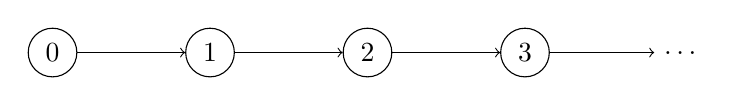
\begin{tikzpicture}
    \node (a) at (0,0) [circle, draw] {0};
    \node (b) at (2,0) [circle,draw] {1}; \node (c) at (4,0)
    [circle,draw] {2}; \node (d) at (6,0) [circle,draw] {3}; \node (e)
    at (8,0) {\ldots}; \draw[->] (a.east) -- (b.west); \draw[->]
    (b.east) -- (c.west); \draw[->] (c.east) -- (d.west); \draw[->]
    (d.east) -- (e.west);
  \end{tikzpicture}
  \caption{A picture of the natural numbers}
  \label{fig:nat-numbers}
\end{figure}


Not all ``stepping stone'' pictures are acceptable.
Figures \ref{fig:NatSigBad1}, \ref{fig:NatSigBad2} and \ref{fig:NatSigBad3} illustrate three ways \emph{not} to picture the natural numbers.

\begin{figure}[h]
\centering
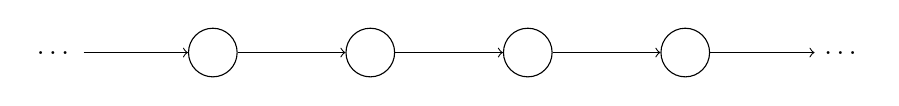
\begin{tikzpicture}
  \node (z) at (-2,0) {\ldots}; 
\node (a) at (0,0) [circle, draw] {\phantom0};
    \node (b) at (2,0) [circle,draw] {\phantom0}; \node (c) at (4,0)
    [circle,draw] {\phantom0}; \node (d) at (6,0) [circle,draw] {\phantom0}; 
    \node (e) at (8,0) {\ldots}; 
    \draw[->] (z.east) -- (a.west); \draw[->] (a.east) -- (b.west); \draw[->]
    (b.east) -- (c.west); \draw[->] (c.east) -- (d.west); \draw[->]
    (d.east) -- (e.west);
%\node (left) at (0,0) [circle,draw] {}; \node (center) at (1,0)
%  [circle,draw] {}; \node (right) at (2,0) [circle,draw] {}; \draw[<-]
%  (left.north east)--(center.north west); \draw[->] (center.south
%  east)--(right.south west); \draw[->] (left.south
%  east)--(center.south west); \draw[<-] (center.north
%  east)--(right.north west);
\end{tikzpicture}
\caption{Nowhere to start}\label{fig:NatSigBad1}

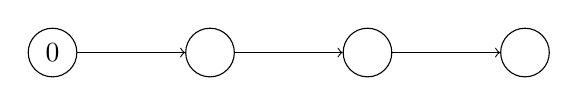
\begin{tikzpicture}
  \node (a) at (1,0) [circle, draw] {0};
    \node (b) at (3,0) [circle,draw] {\phantom0}; \node (c) at (5,0)
    [circle,draw] {\phantom0}; \node (d) at (7,0) [circle,draw] {\phantom0}; 
    \draw[->] (a.east) -- (b.west); \draw[->]
    (b.east) -- (c.west); \draw[->] (c.east) -- (d.west);
\end{tikzpicture}
\caption{Nowhere to go}\label{fig:NatSigBad2}

\begin{tikzpicture}
%    \node (a) at (0,0) [circle, draw] {0};
    \node (b) at (2,0) [circle,draw] {0}; 
    \node (c) at (4,0) [circle,draw] {\phantom0}; 
    \node (d1) at (6,1) [circle,draw] {\phantom0}; 
    \node (d2) at (6,-1) [circle,draw] {\phantom0}; 
    \node (e1) at (8,1) [circle,draw] {\phantom0}; 
    \node (e2) at (8,-1) [circle,draw] {\phantom0};
    \node (f) at (10,0) [circle,draw] {\phantom0};
    \node (g) at (12,0) {\ldots};
%    \draw[->] (a.east) -- (b.west); 
    \draw[->] (b.east) -- (c.west); 
\draw[->] (c.north east) -- (d1.west);
\draw[->] (c.south east) -- (d2.west);
\draw[->] (d1.east) -- (e1.west);
\draw[->] (d2.east) -- (e2.west);
\draw[->] (e1.south east) -- (f.west);
\draw[->] (e2.north east) -- (f.west);
\draw[->] (f.east) -- (g.west);
\end{tikzpicture}
\caption{Forks in the path}\label{fig:NatSigBad3}
\end{figure}

These incorrect pictures can be ruled out by explaining the basic structure of counting. We will ``explain the obvious'' by stating things like this as \emph{postulates}.

%\refstepcounter{axiomCnt}
\begin{postulate}[Basic Structure of Natural Numbers]\label{post:NatSig}
The \newterm{natural numbers} have the following basic structure.
  \begin{itemize}
  \item There is a special natural number. We denote this by $0$.
  \item For any natural number $n$, there is
    a unique \emph{next} natural number. We call this the \newterm{successor of $n$}. 
    In these lectures, we denote the successor of $n$ by $n^\nxt$.
  \end{itemize}
\end{postulate}

According to Postulate \ref{post:NatSig}, $0$, $0^\nxt$, $0^{\nxt\nxt}$, $0^{\nxt\nxt\nxt}$ each denote a natural number. 
Of course, we usually abbreviate them by writing $0$, $1$, $2$, $3$.
But the \emph{characters} $1$, $2$, $3$, etc., are not related to each other in any way.
The notation we are using here makes it completely clear that $0^\nxt$ is the number after $0$, and so on. 
We will want to be able to switch between the familiar ``decimal' notation and ``successor'' notation whenever it is convenient.

\begin{exer}
\begin{multicols}{2}
%\begin{itemize}
\item Convert the following from decimal notation to successor notation.
  \begin{exercise}
  \item $9$
  \item $10$
  \item $4 + 3$
  \item $n + 4$
  \end{exercise}
\item Convert the following to from successor notation to decimal notation.
\begin{exercise}
\item $0^{\nxt\nxt\nxt\nxt}$
\item $n^{\nxt\nxt\nxt\nxt\nxt}$
\item $5^{\nxt\nxt}$
\item $0^\nxt + 0^{\nxt\nxt}$
\end{exercise}
%\end{itemize}
\end{multicols}
\end{exer}

\printbreak

\section{Narrowing the possibilities}

Figures \ref{fig:one-loop} and \ref{fig:two-loop} illustrate 
problems that Postulate \ref{post:NatSig} does not avoid.

\begin{figure}[ht]
  \centering
  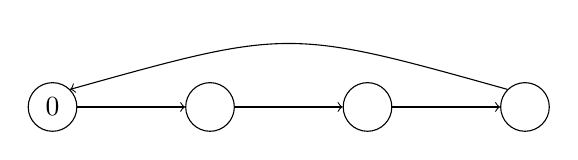
\begin{tikzpicture}
    \node (a) at (0,0) [circle, draw] {$0$}; \node (b) at (2,0)
    [circle,draw] {\phantom{$0$}}; \node (c) at (4,0) [circle,draw]
    {\phantom{$0$}}; \node (d) at (6,0) [circle,draw] {\phantom{$0$}};
    \draw[->] (a.east) -- (b.west); \draw[->] (b.east) -- (c.west);
    \draw[->] (c.east) -- (d.west); \draw[->] (d.north west)
    .. controls (3,1) .. (a.north east);
  \end{tikzpicture}
  \caption{A strange way to count}
  \label{fig:one-loop}
\end{figure}

\begin{figure}[ht]
  \centering
  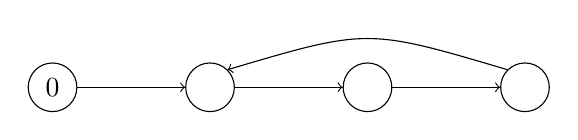
\begin{tikzpicture}
    \node (a) at (0,0) [circle, draw] {$0$}; \node (b) at (2,0)
    [circle,draw] {\phantom{$0$}}; \node (c) at (4,0) [circle,draw]
    {\phantom{$0$}}; \node (d) at (6,0) [circle,draw] {\phantom{$0$}};
    \draw[->] (a.east) -- (b.west); \draw[->] (b.east) -- (c.west);
    \draw[->] (c.east) -- (d.west); \draw[->] (d.north west)
    .. controls (4,.75) .. (b.north east);
  \end{tikzpicture}
  \caption{Another strange way to count}
  \label{fig:two-loop}
\end{figure}
\clearpage

\begin{exer}
\begin{exercise}
\item Explain, in one or two sentences each, why Figures \ref{fig:one-loop} and \ref{fig:two-loop} depict systems that agree with Postulate \ref{post:NatSig}.
\end{exercise}
\end{exer}
\ipadbreak

Figure \ref{fig:one-loop} is flawed because $0$ has a
\emph{predecessor}: a value $n$ satisfying $0^{\nxt\nxt\nxt\nxt} = 0$. Figure
\ref{fig:two-loop} is flawed because an element has two distinct
predecessors: $0^\nxt = 0^{\nxt\nxt\nxt\nxt}$.  We can insist that
these flaws do not happen in the natural numbers. That is, 
we rule them out with axioms.

\begin{postulate}{Nothing Precedes $0$}\label{post:NatZero}
  For every natural number $n$, $n^\nxt\neq 0$.
\end{postulate}

\begin{postulate}{Predecessors are Unique}\label{post:NatPred}
  For any natural numbers $m$ and $n$, if $m^\nxt=n^\nxt$ then $m=n$.
\end{postulate}

These postulates eliminate Figures \ref{fig:one-loop}, \ref{fig:two-loop} and similar pictures.  
But there is still a subtle problem. 
Consider Figure \ref{fig:nonstandard}.

\begin{figure}[h]
  \centering
  \begin{tikzpicture}
    \node (a) at (0,0) [circle, draw] {$0$}; \node (b) at (2,0)
    [circle,draw] {\phantom{$0$}}; \node (c) at (4,0) [circle,draw]
    {\phantom{$0$}}; \node (d) at (6,0) [circle,draw] {\phantom{$0$}};
    \node (e) at (8,0) {\ldots}; \draw[->] (a.east) -- (b.west);
    \draw[->] (b.east) -- (c.west); 
    \draw[->] (c.east) -- (d.west);
    \draw[->] (d.east) -- (e.west);
    % \node (z) at (0,2) {\ldots};
    \node (aa) at (2,2) [circle, draw] {$\star$}; \draw[->] (aa.east)
    .. controls (3.5,3) and (0.5,3) .. (aa.west);
    % \node (bb) at (4,2) [circle,draw] {\phantom{$0$}}; \node (cc) at
    % (6,2) [circle,draw] {\phantom{$0$}}; \node (dd) at (8,2)
    % [circle,draw] {\phantom{$0$}}; \node (ee) at (10,2) {\ldots};
    % \draw[->] (z.east) -- (aa.west); \draw[->] (aa.east) --
    % (bb.west); \draw[->] (bb.east) -- (cc.west); \draw[->] (cc.east)
    % -- (dd.west); \draw[->] (dd.east) -- (ee.west);
  \end{tikzpicture}
  \caption{A model of the natural numbers?}
  \label{fig:nonstandard}
\end{figure}

This picture satisfies the first three postulates. 
Yet, it is not a picture of natural numbers because it has ``extra stuff'' in it ($\star$).

\ipadbreak

To rule out ``extra stuff'', we formulate our final postulate for natural numbers.
We diagnose the problem as follows.
Were we to erase the circle labelled $\star$ and any the arrows leading to and from it, the remaining part of Figure \ref{fig:nonstandard} would still live up to Postulate \ref{post:NatSig}.
This is exactly what we mean by ``extra stuff'': 
elements that can be removed without violating the Postulate \ref{post:NatSig} (the essential structure). 
This leads to our last axiom. 

\begin{postulate}{The Axiom of Induction}\label{post:NatInd}
 No natural numbers can be removed without violating \ref{post:NatSig}.
\end{postulate}

%Believe it or not, the four axioms we have stated here completely
%characterize the standard picture of the natural numbers. In other
%words, any picture that satisfies these axioms will look the same. A
%rigorous proof of this is possible, but not necessary for now.

\begin{exer}
\begin{exercise}
\item Each of the following pictures fails to satisfy either the one or more of our axioms. 
For each, explain which axioms are violated.
\begin{multicols}{2}
\begin{enumerate}
\item
  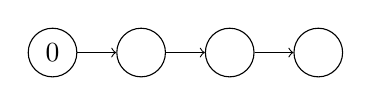
\begin{tikzpicture}[scale=.75]
    \node (a) at (0,0) [circle, draw] {$0$}; \node (b) at (1.5,0)
    [circle,draw] {\phantom{$0$}}; \node (c) at (3,0) [circle,draw]
    {\phantom{$0$}}; \node (d) at (4.5,0) [circle,draw] {\phantom{$0$}};
    \draw[->] (a.east) -- (b.west); \draw[->] (b.east) -- (c.west);
    \draw[->] (c.east) -- (d.west);
  \end{tikzpicture}
\item
  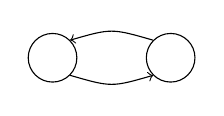
\begin{tikzpicture}[scale=.75]
    \node (a) at (0,0) [circle, draw] {\phantom{$0$}};
    \node (b) at (2,0) [circle, draw] {\phantom{$0$}};
    \draw[->] (a.south east) .. controls (1,-.5) .. (b.south west);
    \draw[->] (b.north west) .. controls (1,.5) .. (a.north east);
  \end{tikzpicture}
\item  
  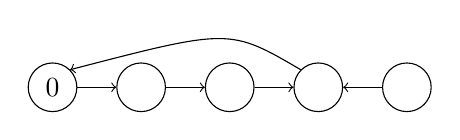
\begin{tikzpicture}[scale=.75]
    \node (a) at (0,0) [circle, draw] {$0$}; \node (b) at (1.5,0)
    [circle,draw] {\phantom{$0$}}; \node (c) at (3,0) [circle,draw]
    {\phantom{$0$}}; \node (d) at (4.5,0) [circle,draw] {\phantom{$0$}};
    \node (e) at (6,0) [circle,draw] {\phantom{$0$}};
    \draw[->] (a.east) -- (b.west); \draw[->] (b.east) -- (c.west);
    \draw[->] (c.east) -- (d.west); \draw[->] (d.north west)
    .. controls (3,1) .. (a.north east);
    \draw[->] (e.west) -- (d.east);
  \end{tikzpicture}
\item
  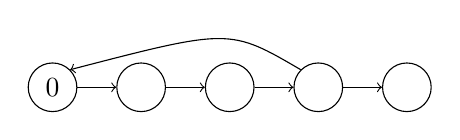
\begin{tikzpicture}[scale=.75]
    \node (a) at (0,0) [circle, draw] {$0$}; \node (b) at (1.5,0)
    [circle,draw] {\phantom{$0$}}; \node (c) at (3,0) [circle,draw]
    {\phantom{$0$}}; \node (d) at (4.5,0) [circle,draw] {\phantom{$0$}};
    \node (e) at (6,0) [circle,draw] {\phantom{$0$}};
    \draw[->] (a.east) -- (b.west); \draw[->] (b.east) -- (c.west);
    \draw[->] (c.east) -- (d.west); \draw[->] (d.north west)
    .. controls (3,1) .. (a.north east);
    \draw[->] (d.east) -- (e.west);    
  \end{tikzpicture}
\end{enumerate}
\end{multicols}

\item\label{exer:cases} I have in mind a picture for the Basic Vocabulary \ref{post:NatSig} and that satisfies Axioms \ref{post:NatZero}
and \ref{post:NatPred}. Furthermore, in that picture, I have in mind and element $n$ for which (a) $n\neq 0$
and (b) $n$ has no predecessor (that is, $n\neq m^\nxt$ for every $m$). Convince me that
the picture fails to satisfy Axiom \ref{post:NatInd}.
\item\label{exer:CyclicModel} Draw three different pictures of situations that satisfies all the postulates except that they fail Postulate \ref{post:NatZero}. So there will be an arrow from a bubble into the bubble $0$. The result must satisfy all other postulates including the Axiom of Induction.
\end{exercise}
\end{exer}

The latest exercise shows that in the natural numbers, if $n\neq 0$, then $n = m^\nxt$ for some $m$. In other
words, every non-zero natural number has a predecessor. 


\chapter{Arithmetic}\label{lec:Arithmetic}


\begin{goals}
\tightlists
\noindent\textbf{Lecture}
\begin{itemize}
\item Present addition and multiplication via defining equations.
\item Practice using the defining equations to calculate sums and products.
\end{itemize}

\noindent\textbf{Study}
\begin{itemize}
  \item Understand addition and multiplication as characterized by defining equations.
  \item Be able to explain how addition and multiplication relate to counting.
  \item Exhibit competence in calculating sums and products from the defining equations.
\end{itemize}
\defaultlists
\end{goals}

Adding and multiplying arise from counting. In this section, we explore how to define them purely in terms of counting.

\ipadbreak
\printbreak

\section{Basic Arithmetic Operations}

We know that addition ``works'' by counting ahead. For example, to \emph{add} $4+5$, we can start with $4$ and then count up five more. Likewise, multiplication ``works'' by counting a number of additions. For example, to multiply $2\cdot 3$ we can add $2$ three times: $2+2+2$. The following definitions capture the idea.
 
\begin{defn}[Arithmetic Operations]\label{def:NatArithmetic}
\noindent The \newterm{sum} of two natural numbers, $m$ and $n$, is a natural number (denoted by $m+n$). For every natural number $m$, the following 
are true:
\begin{align*}
    m + 0     &= m\\
    m + k^\nxt &= (m + k)^\nxt &&\text{for any natural number $k$}
\end{align*}

\noindent The \newterm{product} of two natural numbers, $m$ and $n$, is a natural number 
(denoted by $m\cdot n$). For every natural number $m$, the following are true:
\begin{align*}
  m\cdot 0 &= 0\\
  m\cdot k^\nxt &= m + (m\cdot k) &&\text{for any natural number $k$}
\end{align*}
\end{defn}


A moment's thought about arithmetic should convince you that these equations are reasonable.
Certainly $m+0=m$ and $m\cdot 0 = 0$ should be true for any $m$. 
The second equation for $+$ can be read as saying ``to add $m$ to the successor of $k$, simply add $m$ to $k$, then take the successor.''
The second equation for $\cdot$ can be read as saying ``to multiply $m$ by the successor of $k$, simply multiply $m$ by $k$, and add $m$ to the result.''

The Axiom of Induction ensures that there are indeed unique operations $+$ and $\cdot$ that satisfy the equations.
A proof of this fact is not particularly illuminating right now, so let us agree to take it for granted.

\begin{example}
Do the defining equations for addition really explain how to add? Let's use them to calculate
$4+3$:
\begin{align*}
  4 + 3 &= 4 + 0^{\nxt\nxt\nxt}&&\text{[$3$ abbreviates $0^{\nxt\nxt\nxt}$]}\\
  &= (4 + 0^{\nxt\nxt})^\nxt &&\text{[$m+k^\nxt = (m+k)^\nxt$]}\\
  &= (4 + 0^\nxt)^{\nxt\nxt} &&\text{[Same reason]}\\
  &= (4 + 0)^{\nxt\nxt\nxt} &&\text{[Same reason]}\\
  &= 4^{\nxt\nxt\nxt} &&\text{[$m+0 = m$]}\\
  &= (0^{\nxt\nxt\nxt\nxt})^{\nxt\nxt\nxt} && \text{[$4$ abbreviates $0^{\nxt\nxt\nxt\nxt}$]}\\
  &= 0^{\nxt\nxt\nxt\nxt\nxt\nxt\nxt} && \text{[Remove unneeded parentheses]}\\
  &= 7 &&\text{[$7$ abbreviates $0^{\nxt\nxt\nxt\nxt\nxt\nxt\nxt}$]}
\end{align*}
\end{example}
\ipadbreak

\begin{example}
A product can be calculated similarly. Consider $2\cdot 2$.
\begin{align*}
  2\cdot 2 &= 2\cdot 0^{\nxt\nxt} &&\text{[$2$ abbreviates $0^{\nxt\nxt}$]}\\
           &= 2 + (2\cdot 0^\nxt) &&\text{[$m\cdot k^\nxt = m + (m\cdot k)$]}\\
           &= 2 + (2 + (2\cdot 0))&&\text{[Same reason]}\\
           &= 2 + (2 + 0) &&\text{[$m\cdot 0=0$]}\\
           &= 2 + 2&&\text{[$m+0 = m$]}\\
           &= 2 + 0^{\nxt\nxt}&&\text{[$2$ abbreviates $0^{\nxt\nxt}$]}\\
           &= (2 + 0^\nxt)^\nxt &&\text{[$m+k^\nxt = (m+k)^\nxt$]}\\
           &= (2 + 0)^{\nxt\nxt}&&\text{[Same reason]}\\
           &= 2^{\nxt\nxt} &&\text{[$m+0 = m$]}\\
           &= (0^{\nxt\nxt})^{\nxt\nxt} &&\text{[$2$ abbreviates $0^{\nxt\nxt}$]}\\
           &= 0^{\nxt\nxt\nxt\nxt}&&\text{[Remove unnecessary parentheses]}\\
           &= 4 &&\text{[$4$ abbreviates $0^{\nxt\nxt\nxt\nxt}$]}
\end{align*}
\end{example}

We certainly will not want to calculate this way in real life. 
After all, it took twelve steps just to figure $2\cdot 2=4$. But these
examples and the following exercises show how addition and multiplication are
closely tied to simple counting. 

\ipadbreak

\begin{exer}
\begin{exercise}
\item Calculate these sums, following the previous example to write
  each step of your calculation explicitly. Include the reason for
  each step (as in the previous example).Take care to lay out the
  chain of equalities correctly, and do not skip any steps.
\begin{enumerate}
\item $2+4$
\item $4+2$
\item $3+(3+1)$
\item $(3+3)+1$
\item $0 + 3$
\end{enumerate}

\item Notice that it takes more steps to calculate $2+4$ than $4+2$, even though we know they will produce the same answer. Explain why.

\item Calculate the following values, writing each step explicity. 
 \begin{enumerate}
    \item $2\cdot 3$
    \item $0\cdot 2$
    \item $2\cdot(2\cdot 2)$
    \item $3\cdot(2 + 1)$
    \item $(3\cdot 2) + (3\cdot 1)$
    \end{enumerate}
\item Write a definition of exponentiation via defining equations. Follow the pattern
of definition I have written for addition and multiplication.
\end{exercise}
\end{exer}

\chapter{Laws of Arithmetic}\label{lec:ArithmeticLaws}

\begin{goals}
\noindent\textbf{Lecture}
\begin{itemize}
\item Present the most common Laws of Arithmetic for natural numbers.
\item Explain the method of \emph{proof by simple induction}
\item Prove a representative sample of the laws by simple induction.
\end{itemize}
\noindent\textbf{Study}
\begin{itemize}
\item Become familiar with the common names for the Laws of Arithmetic.
\item Pay particular attention to the Laws of Positivity and Cancellativity (they may be the least familiar to you).
\item Demonstrate the ability to identify the main parts of a proof by simple induction.
\item Demonstrate the ability to construct the parts of a proof by simple induction.
\item Prove the remaining laws for yourself.
\end{itemize}
\end{goals}

Before working the last exercises, you knew that $3\cdot (2+1)$ and $3\cdot 2+ 3\cdot 1$
would come out the same because of a law of arithmetic known as \emph{distributivity}. 
Addition and multiplication satisfy several other laws.

\ipadbreak
\printbreak

%\section{Basic Laws}

The following list summarizes several useful laws of
arithmetic on the natural numbers. They are organized to emphasize
similarities between addition and multiplication.

\begin{laws}
\noindent For any natural numbers, $m$, $n$ and $p$:

\begin{tabular}{lr@{\,}l}
\textbf{Associativity}& $m + (n + p)$       &$= (m+n)+p$\\
                      & $m \cdot(n\cdot p)$ &$= (m\cdot n)\cdot p$\\
\textbf{Commutativity}& $m + n$             &$= n + m$\\
                      &                     &$m\cdot n$ &$= n\cdot m$\\
&&\\ 
\textbf{Identity}     & $m + 0$             &$= m$\\
                      & $m\cdot 1$          &$= m$\\
&\textbf{Positivity}&\multicolumn{2}{c}{if $m + n = 0$ then $m=0$}\\
                                    &\multicolumn{2}{c}{if $m\cdot n = 1$ then $m=1$}\\
&&\\
\textbf{Cancellativity}&\multicolumn{2}{c}{if $m + p = n+p$ then $m=n$}\\
                       &\multicolumn{2}{c}{if $m \cdot p^\nxt = n\cdot p^\nxt$ then $m=n$}\\
&&\\
\textbf{Distributivity}&$m\cdot(n+p)$&$= (m\cdot n) + (m\cdot p)$\\
&&\\
\textbf{Case Distinction}&\multicolumn{2}{c}{if $m\neq 0$ then $m=k^\nxt$ for some $k$}\\
\end{tabular}
\end{laws}
\medskip

Most of these laws are familiar and are listed with their common names. The Law of Case
Distinction was the subject of Lecture \ref{lec:NatNumbers} Exercise \ref{exer:cases}. \emph{Go back and look at that exercise again}.
The Law of Positivity for multiplication is not a common name, but
I have used it to emphasize the analogies between addition and multiplication.
Also Case Distinction does not really have a common name. I made that up.

\ipadbreak

\section{Inductive Proofs}

Suppose we wish to prove that every natural number has some
property. For example, let us suppose we wish to prove that every
natural number is \emph{mimsy}.  I have no idea what a mimsy number
is, but let us try to prove this anyway. We could try proving that $0$
is mimsy, $1$ is mimsy, $2$ is mimsy, and so on.  But this won't work
because our proof will never end. In fact, it is not so obvious that
we, humans with finite minds, can ever prove that some property is
true for \emph{all} natural numbers, since it seems to involve
checking infinitely many individual cases.

The Axiom of Induction provides a way forward in spite of our
limitations.  Suppose we were to show that the mimsy natural numbers
all by themselves constitute a picture of Signature
\ref{post:NatSig}.  Then there could not be any natural numbers
left out, for otherwise, we could erase all the non-mimsy natural
numbers and still have a picture of \ref{post:NatSig}. This
is exactly what the Axiom of Induction forbids: we can not erase
\emph{anything} without breaking the signature.

So to prove that all natural numbers are mimsy, we simply need to
prove that
\begin{itemize}
\item $0$ is mimsy, and
\item for all natural numbers $k$, if $k$ is mimsy so is $k^\nxt$.
\end{itemize}
From these, we conclude that the mimsy natural numbers by themselves form a picture of \ref{post:NatSig}. So the Axiom of Induction ensures that all natural numbers
are mimsy.

%\begin{usage}
%  A proof employing the Axiom of Induction in this way is called a
%  proof \emph{by simple arithmetic induction}, or just a proof \emph{by
%    induction}, for short.  We will see more general forms of
%  induction later.
%\end{usage}

To make inductive proofs easier to understand, we often write them
using a three step outline, as illustrated here.
\begin{itemize}
\item{}[Basis] Prove that $0$ is mimsy.
\item{}[Inductive Hypothesis] Assume that $k$ is mimsy.
\item{}[Inductive Step] Prove that $k^\nxt$ is mimsy. [You may use the
  assumption that $k$ is mimsy in this part of the proof.]
\end{itemize}

More practical examples are next.

\begin{prop}

  \emph{Addition is associative.}

\begin{proof}
  We need to show that $m + (n+p) = (m+n)+p$ for all $m$, $n$ and $p$.
  Let us suppose that $m$ and $n$ are fixed values (not known to us).
  We now prove that the values $p$ for which $m+(n+p) = (m+n)+p$ holds
  form a picture of \ref{post:NatSig}.
  \begin{itemize}
  \item{}[Basis] $m+(n+0) = m+n = (m+n)+0$. Both steps are due to the
    defining equations of $+$.
  \item{}[Inductive Hypothesis] Assume $m+(n+k) = (m+n)+k$.
  \item{}[Inductive Step] We must show that $m+(n+k^\nxt) =
    (m+n)+k^\nxt$. 
    \begin{align*}
      m+(n+k^\nxt) &= m + (n+k)^\nxt &&\text{[Def. of +]}\\
      &= (m+(n+k))^\nxt&&\text{[Same]}\\
      &= ((m+n)+k)^\nxt&&\text{[Inductive Hypothesis]}\\
      &= (m+n)+k^\nxt &&\text{[Def. of $+$]}
    \end{align*}
  \end{itemize}
  Therefore (by the Axiom of Induction), $m+(n+p) = (m+n)+p$ holds for
  all $p$. Since the argument does not depend on any extra assumptions
  about $m$ and $n$, it holds for all $m$ and $n$.
\end{proof}
\end{prop}

\printbreak

In the remainder of this section, we further illustrate the technique of simple arithmetic induction via proofs of other laws of arithmetic.

\ipadbreak

\begin{prop}\label{prop:AddZero}
  $0$ is the identity for addition.

\begin{proof}
  We must prove that $m+0 = m = 0 + m$ for all $m$. The first equality is true by the definition of $+$.
  But the second equality, $m = 0 + m$, is not explicitly one of the defining facts about $+$. So we proceed by induction on $m$.
  \begin{itemize}
  \item{}[Basis] $0+0 = 0$ is true by definition of $+$.
  \item{}[Inductive Hypothesis] Assume $0 + k = k$.
  \item{}[Inductive Step] We must show that $0 + k^\nxt = k^\nxt$.
    \begin{align*}
      0 + k^\nxt &= (0+k)^\nxt &&\text{[Def. of $+$]}\\
      &= k^\nxt &&\text{[Inductive hypothesis]}
    \end{align*}
  \end{itemize}
  Therefore, $0+m=m$ holds for all $m$.
\end{proof}
\end{prop}

\ipadbreak

To prove that addition is commutative, we need an additional fact
about how successor and addition interact. 
Mathematicians use the word \emph{lemma} to indicate that a certain fact is only needed to make others proofs easier and is not necessarily valuable in its own right.

\printbreak

\begin{lem}\label{lem:AddSucc}
  For any $m$ and $n$, $(m + n)^\nxt = m^\nxt + n$.

 \begin{proof}
   By induction on $n$:
   \begin{itemize}
   \item{}[Basis]
     \begin{align*}
       (m + 0)^\nxt &= m^\nxt     &&\text{[Def. of $+$]}\\
       &= m^\nxt + 0 &&\text{[Def. of $+$]}
     \end{align*}
   \item{}[Inductive Hypothesis]
    Assume $(m + k)^\nxt = m^\nxt + k$ for some $k$.
   \item{}[Inductive Step]
    We must show that $(m + k^\nxt)^\nxt = m^\nxt + k^\nxt$.
    \begin{align*}
      (m + k^\nxt)^\nxt &= ((m + k)^\nxt)^\nxt && \text{[Def. of $+$]}\\
                     &= (m^\nxt + k)^\nxt &&\text{[Inductive Hypothesis]}\\
                     &= m^\nxt + k^\nxt   &&\text{[Def. of $+$]}
    \end{align*}
   \end{itemize}
So $(m + n)^\nxt = m^\nxt + n$. Because the proof does not depend on any assumption about $m$, it is valid
for all $m$.
 \end{proof}
\end{lem}

Roughly speaking this lemma permits us to move $\nxt$ anywhere within an addition: $m^\nxt + n = (m+n)^\nxt = m+n^\nxt$. So we are free to move a successor ``out of the way'' whenever we need to. The next proof illustrates the point.

\printbreak

\begin{prop}

  \emph{Addition is commutative.}

\begin{proof}
  We need to show that $m+n = n + m$ for all $m$ and $n$.  This time,
  the proof is by induction on $m$. Fix a value for $n$.
  \begin{itemize}
  \item{}[Basis] $0 + n = n = n + 0$ holds because of Proposition
    \ref{prop:AddZero} and the definition of $+$.
  \item{}[Inductive Hypothesis] Assume that $k + n = n + k$ for some
    $k$.
  \item{}[Inductive Step] We must show that $k^\nxt + n = n + k^\nxt$.
    \begin{align*}
      k^\nxt + n &= (k + n)^\nxt&&\text{[Lemma \ref{lem:AddSucc}]}\\
      &=  (n+k)^\nxt&&\text{[Inductive Hypothesis]}\\
      &= n + k^\nxt&&\text{[Def. of $+$]}
    \end{align*}
  \end{itemize}
  Therefore, $m + n = n + m$ for all $m$. Since this argument does not
  depend on any assumptions about $n$, it is valid for all $n$.
\end{proof}
\end{prop}

The next law may be less familiar to you. Roughly, it says that we can ``subtract'' equals and get equals. But note that actual subtraction does not always make sense for natural numbers. We can not, for example, say what $5-7$ means without introducing negative numbers.

\printbreak

\begin{prop}
  \emph{Addition is cancellative.}

\begin{proof}
  We need to prove that if $m + p= n+p$, then $m=n$.  This proof is a little subtler than the previous ones. But notice that is
  still follows the same form.
  
  The proof is by induction on $p$. Assume that $m$ and $n$ are some fixed natural numbers.
  \begin{itemize}
  \item{}[Basis] Suppose $m+0 = n+ 0$. Then immediately by definition
    of $+$, $m=n$.
  \item{}[Inductive Hypothesis] Assume that the following statement is true for some $k$: if $m + k = n + k$ then $m=n$.
  \item{}[Inductive Step] We must show that 
    if $m+k^\nxt = n+k^\nxt$ then $m=n$. Suppose $m+k^\nxt = n + k^\nxt$ [call this (*) for reference]. Then
    \begin{align*}
      (m+k)^\nxt & = m + k^\nxt &&\text{[Def. of $+$]}\\
      & = n + k^\nxt &&\text{[By the supposition (*)]}\\
      & = (n+k)^\nxt &&\text{[Definition of $+$]}
    \end{align*}
    Hence, by Axiom \ref{ax:NatPred} $m+k=n+k$. So by the Inductive Hypothesis, $m=n$.
  \end{itemize}
  Therefore, $m + p = n + p$ implies $m = n$ for all $p$. Since this argument does not
depend on any assumptions regarding $m$ and $n$, it is valid for all $m$ and $n$.
\end{proof}
\end{prop}
\ipadbreak

To prove that multiplication is commutative and cancellative, we will
need the following technical facts (analogous to Proposition
\ref{prop:AddZero} and Lemma \ref{lem:AddSucc}).

\begin{lem}\label{lem:MultZero}
  For any $n$, $0\cdot n = 0$

  \begin{proof}
    The proof is by induction on $n$.
    \begin{itemize}
    \item{}[Basis] $0\cdot 0 = 0$ by definition of $\cdot$.
    \item{}[Inductive Hypothesis] Assume that $0\cdot k = 0$ for some
      $k$.
    \item{}[Inductive Step] We must show that $0\cdot k^\nxt = 0$.
      \begin{align*}
        0\cdot k^\nxt &= 0 + 0\cdot k &&\text{[Definition of $\cdot$]}\\
        &= 0 + 0 &&\text{[Inductive Hypothesis]}\\
        &= 0&&\text{[Definition of $+$]}
      \end{align*}
    \end{itemize}
  \end{proof}
\end{lem}

\ipadbreak

\begin{lem}\label{lem:MultSucc}
  For any $m$ and $n$, $m^\nxt \cdot n = m\cdot n + n$

 \begin{proof}
   The proof is by induction on $n$.
   \begin{itemize}
   \item{}[Basis] $m^\nxt\cdot 0 = 0 = 0+0 = m\cdot 0 + 0$ all follow
     from the definitions of $+$ and $\cdot$.
   \item{}[Inductive Hypothesis] Assume that $m^\nxt\cdot k = m\cdot k +
     k$ for some $k$.
   \item{}[Inductive Step] We must show that $m^\nxt\cdot k^\nxt =
     m\cdot k^\nxt + k^\nxt$.
     \begin{align*}
       m^\nxt\cdot k^\nxt &= m^\nxt + m^\nxt\cdot k &&\text{[Exercise]}\\
       &= (m + m^\nxt\cdot k)^\nxt &&\text{[Exercise]}\\
       &= (m + (m\cdot k + k))^\nxt && \text{[Exercise]}\\
       &= ((m+ m\cdot k) + k)^\nxt &&\text{[Exercise]}\\
       &= (m\cdot k^\nxt + k)^\nxt &&\text{[Exercise]}\\
       &= m\cdot k^\nxt + k^\nxt &&\text{[Exercise]}
     \end{align*}
   \end{itemize}
 \end{proof}
\end{lem}

Some of the other laws are left as exercises.

\printbreak

\begin{exer}
  \begin{exercise}
\item Prove that $1$ is the identity for multiplication. That is $1\cdot m = m  = m\cdot 1$.
\item Write out the entire proof of Lemma \ref{lem:MultSucc} providing the justifications for each line of the equational calculation in the Inductive Step.
\item Prove that multiplication distributes over addition [$m\cdot
  (n+p) = m\cdot n + m\cdot p$] by induction on $p$.  You can use the any of the lemmas and propositions we have
  already proved.
  \begin{enumerate}
  \item Prove the basis: $m\cdot(n+0) = m\cdot n + m\cdot 0$.
  \item Write the inductive hypothesis.
  \item Prove the inductive step: $m\cdot(n+k^\nxt) = m\cdot n +
    m\cdot k^\nxt$
  \end{enumerate}
 
\item Prove that multiplication is associative [$m\cdot(n\cdot p) =
  (m\cdot n)\cdot p$] by induction on $p$.
  \begin{enumerate}
  \item Prove the basis: $m\cdot (n\cdot 0) = (m\cdot n)\cdot 0$.
  \item Write the inductive hypothesis.
  \item Prove the Inductive Step: $m\cdot (n\cdot k^\nxt) = (m\cdot
    n)\cdot k^\nxt$. 
    Hint: Use the Law of Distribution, which you just
    proved.
  \end{enumerate}

\item Prove that multiplication is commutative. 
Hint: Use the two Lemmas we proved right before these exercises.

  \end{exercise}
\end{exer}
%\ipadbreak
%
%For the record, we don't prove the cancellation law for multiplication here. It is similar to the others but a bit trickier. Nevertheless, the proof does not provide a new insight, so we omit it. 
%
%\begin{prop}
%
%  \emph{If $m\cdot p^\nxt = n\cdot p^\nxt$, then $m=n$.}
%
%\begin{proof}
%  The proof is by induction on $p$.
%  \begin{itemize}
%  \item{}[Basis] Suppose $m\cdot 0^\nxt = n\cdot 0^\nxt$. That is, $m\cdot 1=n\cdot 1$. Direct calculations show that $1$ is the identity for multiplication, so $m=n$. 
%  \item{}[Inductive Hypothesis] Assume that for some $k$, the following is true:
%    if $m\cdot k^\nxt = n\cdot k^\nxt$, then $m=n$.
%  \item{}[Inductive Step] Suppose that $m\cdot k^{\nxt\nxt} = n\cdot
%    k^{\nxt\nxt}$. Then
%    \begin{align*}
%      m\cdot k^{\nxt} + m &= k^\nxt\cdot p^\nxt &&\text{[By assumption]}\\
%      &= k\cdot p^\nxt + p^\nxt &&\text{[Lemma \ref{lem:MultSucc}]}\\
%      &= (k\cdot p^\nxt + p)^\nxt &&\text{[Definition of $+$]}\\
%      &\neq 0 &&\text{[Axiom Nat \ref{ax:NatZero}]}
%    \end{align*}
%    Consequently, $m\neq 0$, for otherwise we would have $m\cdot
%    p^\nxt = 0$. Since $m$ is not equal to $0$, it is equal to some
%    successor (by the Case Distinction Law). Let $j$ be the predecessor of $m$,
%	so that $j^\nxt=m$. Then
%    \begin{align*}
%      j\cdot p^\nxt + p^\nxt & = m\cdot p^\nxt &&\text{[Lemma \ref{lem:MultSucc}]}\\
%      &= k^\nxt \cdot p^\nxt &&\text{[By supposition]}\\
%      &= k\cdot p^\nxt + p^\nxt &&\text{[Lemma \ref{lem:MultSucc}]}
%    \end{align*}
%    Because addition is cancellative, $j\cdot p^\nxt = k\cdot
%    p^\nxt$. Now, the Inductive Hypothesis ensures that $j=k$. Hence
%    $m = j^\nxt = k^\nxt$.
%  \end{itemize}
%\end{proof}
%\end{prop}

% 1
%\chapter{Lists}

Natural numbers constitute an important example of something more
general, where objects are built up from simpler
ones. The Axiom of Induction captures the idea of building ``up''
and provides an important method for proving facts about natural
numbers.

In this lecture, we develop an analogous way to think about \emph{lists}. 

\begin{goals}
\noindent \textbf{Lecture Goals}
\begin{itemize}
\item Introduce a formal counterpart to the informal concept of a list
\item Emphasize the close analogy between lists and natural numbers
\item Introduce basic operations on lists.
\end{itemize}

\noindent\textbf{Study Goals}
\begin{itemize}
\item Demonstrate facility with basic list manipulation including calculating length and 
concatenation of lists.
\end{itemize}
\end{goals}

\section{Lists}

\ignore{
For natural numbers $0$ and $n^\nxt$ are the only ways to construct
natural numbers. Operations like addition and multiplication are
defined in terms of $0$ and ${}^\nxt$, so they do not contribute directly
to the \emph{construction} of natural numbers.

We refer to $0$ and $\nxt$ as \emph{constructors}.  Axioms
\ref{ax:NatZero} and \ref{ax:NatPred} spell out how these
constructors behave.  Axiom \ref{ax:NatZero} captures the idea that
each constructor is entirely different from the other: $0\neq n^\nxt$.
Axiom \ref{ax:NatPred} captures the idea that ${}^\nxt$ constructs
distinct natural numbers from distinct natural numbers: $m^\nxt =
n^\nxt$ implies $m=n$.

So the basic ingredients of natural numbers are the constructors $0$
and ${}^\nxt$ with the understanding that (a) they each produce
different results and (b) from different ingredients, ${}^\nxt$
produces different results. In fact, point (b) also applies to $0$
trivially, because $0$ does not use any ingredients.

We can summarize everything we want to say about natural numbers
concisely in the following way.

\begin{definition}
  The \emph{natural numbers} are defined \emph{inductively} by
  \begin{align*}
    n &\defeq 0 \mathrel{\mid} n^\nxt
  \end{align*}
\end{definition}

In this notation, the vertical bar separates the different constructors for
natural numbers.  The first constructor ($0$) does not depend on
anything else. The second constructor depends on a natural number $n$
and produces a new one $n^\nxt$. So this gives a very concise description of the signature of natural numbers.
Implicitly, this notation is meant to
indicate that the two alternatives are completely distinct. This is
Axiom \ref{ax:NatZero}.  Also implicitly, ${}^\nxt$ is meant to produce
distinct results from distinct $n$'s.  This is Axiom
\ref{ax:NatPred}.  By saying that this defines natural numbers
\emph{inductively}, we also implicitly include the Axiom of
Induction. Namely, no natural numbers can be removed without violating
the structure.

Other kinds of mathematical objects can be defined by inductively by
describing their construction. Indeed, many important types of data in computing
are defined inductively. 
}

In this section, we concentrate on the fundamental concept of \emph{lists}. The idea is really meant to
be the familiar one, so a list of ``to do'' items is a list. The alphabetized names on a class roster is a list. 
We will write lists using square brackets. So for example, $[2,3,5,7]$ is the list of 
the prime numbers less than $10$ in ascending order. For lists, we expect the order to matter. 
So $[7,5,3,2]$ is a different list.

Something that occurs on a list is called an \emph{item} of the list. We can even
specify where it is. So we can talk about the ``first'', ``second'' item, and so on, 
assuming the list has enough items. 

Because we have already agreed that natural numbers begin with $0$, it turns out to make
many things easier if we change the way we talk about items on a list to gibe with the natural
numbers. So instead of refering to the ``first'' item, we might call it the ``initial'' item.
Furthermore, we will number them to start with $0$. What I mean is that if $L=[2,3,5,7]$,
we will write $L_0$, $L_1$, $L_2$, $L_3$ for the elements $2$, $3$, $5$, $7$, respectively. 
In short, the ``initial'' item is indexed by the ``initial'' natural number $0$. The next item after that is indexed by next natural number, $0^\nxt$,
and so on.

Like natural numbers, lists can be built up by starting with an empty list and incrementally adding items. We have choices 
for how we might formalize the idea. We will follow a standard that has developed in computer science. Clearly, since we use 
square brackets to punctuate lists, the empty list should be written as $[\,]$. To add an item to a list, we will conventionally
put it on the front.  

Given the list $[x,y,z]$, we may build a new list with initial item $w$ and the given list as the rest, resulting in $[w,x,y,z]$.
The operation of \emph{prepending} an item to a list is denoted by a colon (:). 
So $w:[x,y,z]$ \emph{is} the list $[w,x,y,z]$.

The empty list, together with prepending items, gives us a way to construct any list we want.

\ipadbreak

\begin{example}
  Here are some examples.
  \begin{itemize}
  \item $5:6:[4,5]$ is the same as $5:[6,4,5]$, which is the same as
    $[5,6,4,5]$.
  \item $[\,]$ is the empty list
  \item $1:[\,]$ is the same as $[1]$
  \item $1:2:3:4:[\,]$ is the same as $[1,2,3,4]$.
  \end{itemize}
\end{example}

Notice that every list is either empty ($[\,]$) or not. If not, it has
the form $x:L$ where $x$ is the initial item and $L$
is the rest of the list. This suggests a signature for lists, not so different from
the signature for natural numbers.

\begin{signature}{sig:list}
	Lists have the following basic structure.
	  \begin{itemize}
	  \item There is a special list, which we call \emph{the empty list} and denote by $[\,]$.
	  \item For any thing $x$ and any list $L$, there is another list, obtained by \emph{prepending} $x$ to $L$. We denote
	  the result by $x:L$.
	  \end{itemize}
\end{signature}

As with the natural numbers, we need to think about axioms that prevent strange behavior. These are exactly analogous to the
axioms of natural numbers. First, $[\,]$ can not be obtained by adding a new initial item to another list. So

\begin{axiom}
	For any list $L$ and any thing $x$, $[\,]\neq x:L$.
\end{axiom}

Likewise, a list that is not empty can only be built one way.

\begin{axiom}
	For any things $x$ and $y$ and lists $L$ and $M$, if $x:L = y:M$, then $x=y$ and $L=M$.
\end{axiom}

For example, if I tell you that $[2,3,4,5] = x:L$, then you know immediately that $x=2$ and $L=[3,4,5]$.

Finally, lists need an induction axiom that ensures that all lists are built up from $[\,]$.


\begin{axiom}\label{ax:NatInd}
	[The Axiom of List Induction] No lists can be removed without violating \ref{sig:list}.
\end{axiom}

This axiom justifies conducting proofs about all lists by a scheme almost identical to simple arithmetic induction.
That is, to prove some property is true about all lists, it is enough to show
\begin{itemize}
\item{}[Basis] The property is true about $[\,]$.
\item{}[Inductive Hypothesis] Assume that the property is true for from list $K$.
\item{}[Inductive Step] Prove that for any thing $x$, the property is true about $x:K$. [You may use the
  assumption about $K$ in this part of the proof.]
\end{itemize}

Operations on lists can now also be defined by schemes similar to how 
we defined addition and multiplication on natural numbers. For example,
every list has a length. Writing $\len(L)$ for the length of a list,
$\len([2,3,4]) = 3$.  A precise definition is now easy to formulate.

\begin{definition}
  For a list $L$. the \emph{length} of $L$, denoted by $\len(L)$, is
  the natural number. This satisfies the following equalities.
  \begin{align*}
    \len([\,]) &= 0\\
    \len(x:L) &= len(L)^\nxt
  \end{align*}
\end{definition}

\begin{example}
  \begin{align*}
    \len([2,3,4]) &= \len(2:[3,4])\\
    &= \len([3,4])^\nxt\\
    &= \len(3:[4])^\nxt\\
    &= \len([4])^{\nxt\nxt}\\
    &= \len(4:[\,])^{\nxt\nxt}\\
    &= \len(,])^{\nxt\nxt\nxt}\\
    &= 0^{\nxt\nxt\nxt}\\
    &= 3
  \end{align*}
\end{example}

\ipadbreak

Another common operation on lists is \emph{concatenation}:
$[2,3,4]\otimes[4,1,3] = [2,3,4,4,1,3]$, whereby the two lists are simply glued together in their original orders.  This is defined precisely by
the following.

\begin{defn}
  For lists $L$ and $M$, their \emph{concatenation}, denoted by
  $L\otimes M$, is a list. For all lists $M$, the following are true.
  \begin{align*}
    [\,]\otimes M &= M\\
    (x:K)\otimes M &= x:(K\otimes M) & \text{for any thing $x$ and any list $K$}
  \end{align*}
\end{defn}

\begin{example}
  To calculate $[4,5,2,1] \otimes [3,4,1]$, we can follow a method similar to arithmetic:
  \begin{align*}
    [4,5,2,1]\otimes[3,4,1] &= (4:5:2:1:[\,])\otimes[3,4,1] & \text{[$[4,5,2,1]$ abbreviates $4:5:2:1:[\,]$]}\\
                    &= 4:((5:2:1:[\,])\otimes[3,4,1]) &\text{[Def. of $\otimes$]}\\
                    &= 4:5:((2:1:[\,])\otimes[3,4,1]) & \text{[Same]}\\
                    &= 4:5:2:((1:[\,])\otimes[3,4,1]) &\text{[Same]}\\
                    &= 4:5:2:1:([\,]\otimes[3,4,1])  &\text{[Same]}\\
                    &= 4:5:2:1:[3,4,1] &\text{[Same]}\\
                    &= [4,5,2,1,3,4,1]                &\text{[Abbreviation]}
  \end{align*}
\end{example}

\ipadbreak
Now we can prove some useful facts about lists.

\begin{lemma}
  On lists, $[\,]$ is the identity for $\otimes$,

\begin{proof}
  By definition
  $[\,]\otimes L = L$ always true.  But $[\,]$ must also 
  satisfy
  $L\otimes[\,] = L$ always. We can proceed by
  induction on $L$. The proof should look familiar (see the proof of
  Lemma \ref{lem:AddZero}).

  \begin{itemize}
  \item{}[Basis] $[\,]\otimes [\,] = [\,]$ is true by definition of
    $\otimes$.
  \item{}[Inductive Hypothesis] Assume $K\otimes[\,] = K$ for some list
    $K$.
  \item{}[Inductive Step]  Suppose $x$ is some thing. We need to show that $(x:K) \otimes [\,] = x:K$. 
    \begin{align*}
       (x:K)\otimes [,\] &= x:(K\otimes[\,]) &\text{[by definition of $\otimes$]}\\
	                   &= x:K &\text{[by the Inductive Hypothesis]}   	
    \end{align*}
  \end{itemize}
  Thus (by the Axiom of List Induction), the lists for which $L\otimes [\,] = L$ constitute all lists.
\end{proof}
\end{lemma}


\ipadbreak

\begin{lemma}
On lists, $\otimes$ is associative.

\begin{proof}
We prove $L\otimes(M\otimes N) =
  (L\otimes M)\otimes N$ using induction on $L$. This should look
  familiar. It is almost identicial to the proofs that addition and
  multiplication are associative.

  \begin{itemize}
  \item{}[Basis] $[\,]\otimes(M\otimes N) = M\otimes N = ([\,]\otimes M)\otimes
    N$. Both steps are by the definition of $\otimes$.
  \item{} [Inductive hypothesis] Suppose $K\otimes(M\otimes N) = (K\otimes
    M)\otimes N$ for some particular list $K$.
  \item{} [Inductive step]
    \begin{align*}
      (x:K)\otimes (M\otimes N) &= x:(K\otimes (M\otimes N)) &\mbox{Def. of $\otimes$}\\
      &= x:((K\otimes M)\otimes N) &\mbox{Inductive Hypothesis}\\
      &= (x:(K\otimes M))\otimes N &\mbox{Def. of $\otimes$}\\
      &= ((x:K)\otimes M)\otimes N &\mbox{Def. of $\otimes$}
    \end{align*}
  \end{itemize}
  So $L\otimes(M\otimes N) = (L\otimes M)\otimes N$ is true for all $L$. Since the proof
  does not depend on any special propertis of $M$ and $N$ (except that they are both lists),
  the result is true for all lists $M$ and $N$.
\end{proof}
\end{lemma}

\ipadbreak

Here is another nice fact that we can prove by induction relating
length to concatenation.

\begin{lemma}
  For any lists $L$ and $M$, $\len(L\otimes M) = \len(L)+\len(M)$.

\begin{proof} [This claim is probably fairly obvious to
  you. Nevertheless, to illustrate the technique of list
  induction again, we prove it explicitly.]
  \begin{itemize}
  \item {}[Basis] $\len([\,]) + \len(M) = 0 + \len(M) = \len(M) =
    \len([\,]\otimes M)$. These are by definition of $\otimes$ and $+$.
  \item{} [Inductive Hypothesis] Suppose $\len(K\otimes M) = \len(K)
    + \len(M)$ holds for some particular list $K$.
  \item{} [Inductive Step]
    \begin{align*}
      \len((x:K)\otimes M) &= \len(x:(K\otimes M)) &\mbox{Def. of $\otimes$}\\
      &= \len(K\otimes M)^\nxt &\mbox{Def. of $\len$}\\
      &= (\len(K)+\len(M))^\nxt &\mbox{Inductive Hypothesis}\\
      &= \len(K)^\nxt + \len(M) &\mbox{Lemma \ref{lem:AddSucc}}\\
      &= \len(x:K) + \len(M) &\mbox{Def. of $\len$}
    \end{align*}
  \end{itemize}
\end{proof}
\end{lemma}

Often we will use a list somewhat informally without all the
punctuation. For example, we might say ``Consider a list $a_0$, $a_1$,
\ldots, $a_{n-1}$ of real numbers.'' If we do not intend to use the list
itself for anything special, but only want to think about the numbers
$a_0$ through $a_n$, then there is no need to be formal about
it. Also, there is no harm in writing something like this: $a_5$,
$a_6$, $a_7$, $a_8$, where the indices start at
$5$. The default is to start at $0$, but that is merely a convention.

\section{List Itemization}

In a list $L$, the items are in order. So we can refer to items by
their position in the list. There are two standards in mathematics
for doing this. Either we start counting from $1$ or from $0$.
Although it may seem unintuitive to start from $0$ (meaning that
the ``initial'' item of a list is item number $0$), this actually 
makes many calculations simpler. For that reason, most programming
languages use this convention for a lists and arrays. So I will consistently
start with $0$.

The idea can be made precise as follows.

\begin{defn}\label{def:ListIndices}
Suppose $L$ is a list and $i<\len(L)$. Then $L_i$ is an item on the list
defined as follows.
\begin{align*}
  [\,]_i &\text{ is never defined because $0\not<\len([\,])$}\\
  (x:L)_0 &\defeq x\\
  (x:L)_{k^\nxt} &\defeq L_k &\text{provided that $L_k$ is defined}
\end{align*}
\end{defn}

This is a precise way of explaining that in a list, for example $L=[a,b,c,d,e]$,
we can refer to an item by its \emph{index}, so that $L_0 = a$, $L_1=b$ and so on,
up to $L_4 = e$. Notice that $L_k$ is undefined if $k\geq \len(L)$.

\ipadbreak

\begin{example}
Suppose $L=[a,b,c,d,e]$. We can calculate $L_3$ 
explicitly step by step.
\begin{align*}
L_3 &= [a,b,c,d,e]_3\\
    &= (a:b:c:d:e:[\,])_{0^{\nxt\nxt\nxt}}\\
    &= (b:c:d:e:[\,])_{0^{\nxt\nxt}}\\
    &= (c:d:e:[\,])_{0^\nxt}\\
    &= (d:e:[\,])_0\\
    &= d
\end{align*}

Of course, this is just a very careful (you might even say fussy) way to find item number $3$ in the list. In every day use, we humans would not do this. We would simply count forward
from the beginning of the list.

\end{example}

\ipadbreak

\begin{exercises}
 % \item Suppose $L$ is a list and $i<\len(L)$. Then it makes sense to 
  %      think about the list in which $L_i$ is removed. For example,
   %     for $L = [a, b, c]$, removing $L_1$ results in the list $[a,c]$.
    %    Let us denote the result of removing item $i$ from list $L$ as
     %   $L\setminus i$. So $[a,b,c]\setminus i = [a,c]$.

    %    In this exercise, you define $L\setminus i$ explicitly. Explain your answers for each point.
    %    \begin{enumerate}
    %    \item Should $[\,]\setminus 0$ be defined? If not, why not? If so, what should it be?
    %    \item What should $(x:L)\setminus 0$ be?
    %    \item What should $(x:L)\setminus k^\nxt$ be? When should it be defined and undefined?
    %    \item Now write your definition for $L\setminus i$ in a layout similar to Definition \ref{def:ListIndices}.
    %    \end{enumerate}
  \item Suppose $L = [3,2,3,3,5]$ and $M = [0,1,2,3,4,5]$. Calculate the following explicitly step by step.
  \begin{enumerate}
  \item $\len(L)$
  \item $L_4$
  \item $(L\otimes M)_9$
%  \item $L\setminus 4$.
%  \item $((M\otimes L)\setminus 3)_5$
  \end{enumerate}
\end{exercises}

\ipadbreak

\section{Lists of a Particular Type}

We will commonly need to consider lists in which all elements are similar, such as a list consisting of natural numbers. For example,
because we know how arithmetic operations work on natural numbers, we can also define operations on lists of natural numbers using 
arithmetic. Similar extensions are possible for other operations defined on other types of elements.

To illustrate, suppose $L$ is a list of natural numbers. We can define the \emph{sum} of items on the list
in the obvious way, so that the sum of the list $[2,3,4]$ is $2+3+4 = 9$. We make this precise with the following.

\begin{defn}
	For a list $L$ of natural numbers, the \emph{sum of $L$}, denoted by $\sum L$, is a natural number, satisfying
	\begin{align*}
	\sum[\] &= 0\\
	\sum m:L &= m + \sum L &\text{for any natural number $m$ and any list of natural numbers $L$}
	\end{align*}
\end{defn}

We will introduce variations and extrensions of this notation this later. For now, we look only at lists. 

\begin{exercises}
\item Prove using list induction that for any lists of natural numbers,
\[\sum L + \sum M = \sum (L\otimes M)\]
\item Define the product of lists of natural numbers, following the pattern of our definition for $\sum L$. The standard notation
for a product is $\prod L$. The result should be that $\prod[2,3,4]$ equals $24$. Pay close attention the base case $\prod[\,]$.
\item Using your definition of products, prove by list induction that for any lists of natural numbers,
\[\prod L\cdot \prod M = \prod(L\otimes M)\]. 
\end{exercises}

We can also consider lists of integers, lists of real numbers, and so on. We can even think about lists of lists.
For example, $[[2,3,4],[4,3,2],[5]]$ is a list consisting of two items: $[2,3,4]$, $[4,3,2]$ and $[5]$. Written this using
:, this is list is $[2,3,4]:[4,3,2]:[5]:[\,]$. Suppose we have a list of lists like this we can define the
concatenation of all the items. For this example, the result should be $[2,3,4,4,3,2,5]$. The definition of this
is exactly analogous to sums and products.

\begin{defn}
	For a list $\mathcal L$ of lists, the \emph{fold of $\mathcal L$}, denoted by $\bigotimes \mathcal L$, is a list, satisfying
	\begin{align*}
	\bigotimes[\,] &= [\,]\\
	\sum M:\mathcal L &= M \otimes \otimes \mathcal L &\text{for any list $M$ and any list of lists $\mathcal L$}
	\end{align*}
\end{defn}

Compare the definitions of $\sum$, $\prod$ and $\otimes$. They differ only in terms of (i) what is the result for an empty list
and (ii) what binary operation is used in the second equation.

Suppose we are given a list $\mathcal L$ of lists of natural numbers (like the example just above the latest definition). Then its fold is a list of natural numbers. So this can be summed. That is, $\bigotimes \mathcal L$ is a list of natural numbers, and $\sum(\otimes \mathcal L)$ is a natural number. But we might also apply the summation operation to each list on $\mathcal L$ separately, resulting in another list of natural numbers.
The idea of applying an operation to each element of a list is called ``mapping''. In this case, we intend to ``map'' the operation $\sum$
across lists of lists of natural numbers. Here is a suitable definition.

\newcommand{\map}{\mathord{\textsf{map}}}
\begin{defn}
	For a list $\mathcal L$ of lists of natural numbers, the \emph{mapping of $\sum$ on $\mathcal L$}, denoted by $\map_\sum(\mathcal L)$
	is a list of natural numbers, satisfying
	\begin{align*}
	\bigotimes[\,] &= [\,]\\
	\sum M:\mathcal L &= ()\sum M): \mathcal L &\text{for any list of natural numbers $M$ and any list of lists of natural numbers $\mathcal L$}
	\end{align*}
\end{defn}

\begin{exercises}
	\item Calculate $\sum(\otimes[[3,4,5],[6,3]])$.
	\item Calculate $\map_\sum([[3,4,5],[6,3]])$.
	\item Calculate $\sum(\map_\sum([[3,4,5],[6,3]]))$.
	\item Prove that $\sum(\otimes\mathcal L) = \sum(\map_\sum(\mathcal L))$ for any list of lists of natural numbers $\mathcal L$.
\end{exercises}

\section{An Efficient Presentation of Natural Numbers and Lists}

The structure of natural numbers and the structure of lists are very similar. This similarity can be exploited to 
develop a simple way of summarizing their properties.

For natural numbers, $0$ and $n^\nxt$ are the only ways to construct
natural numbers. Operations like addition and multiplication are
defined in terms of $0$ and ${}^\nxt$, so they do not contribute directly
to the \emph{construction} of natural numbers. So
we refer to $0$ and $\nxt$ as \emph{constructors}.  

Axioms \ref{ax:NatZero} and \ref{ax:NatPred} spell out how these
constructors behave.  Namely, Axiom \ref{ax:NatZero} captures the idea that
the two constructors are entirely different from the other: $0\neq n^\nxt$.
Axiom \ref{ax:NatPred} captures the idea that ${}^\nxt$ constructs
distinct natural numbers from distinct natural numbers: $m^\nxt =
n^\nxt$ implies $m=n$ (or equivalently, $m\neq n$ implies $m^\nxt\neq n^\nxt$).

So the basic ingredients of natural numbers are the constructors $0$
and ${}^\nxt$ with the understanding that (a) each produces
different results and (b) from different ingredients, ${}^\nxt$
produces different results. In fact, point (b) also applies to $0$
trivially, because $0$ does not use any ingredients.

We can summarize everything we want to say about natural numbers
concisely in the following way.

\begin{defn}
  The \emph{natural numbers} are defined \emph{inductively} by
  \begin{align*}
    n &\defeq 0 \mathrel{\mid} n^\nxt
  \end{align*}
\end{defn}

In this notation, the vertical bar separates the different constructors for
natural numbers.  The first constructor ($0$) does not depend on
anything else. The second constructor depends on a natural number $n$
and produces a new one $n^\nxt$. So this gives a very concise description of the signature of natural numbers.
Implicitly, this notation is meant to
indicate that the two alternatives are completely distinct. This is
Axiom \ref{ax:NatZero}.  Also implicitly, the notation is meant indicate that $n^\nxt$
produces distinct results from distinct $n$'s.  This is Axiom
\ref{ax:NatPred}.  By declaring saying that this defines natural numbers
\emph{inductively}, we also mean that no natural numbers can be removed without violating
the signature.

Now let's consider lists. Again, there are two ways to construct lists. $[\,]$ and $x:L$ for any thing $x$
and any list $L$. Likewise, the constructrs are distinct, and $x:L=y:M$ is true if and only if
both $x=y$ and $L=M$. So we can encapsulate the definition of lists similarly.

\begin{defn}
    The \emph{lists} are defined \emph{inductively} by
    \begin{align*}
      L &\defeq [\,] \mathrel{\mid} x:L & \text{for any thing $x$}
    \end{align*}
\end{defn}

Later in the course, we will make definitions like this rigorous, and will give other similar ones. For now, I just draw your attention to the similarity, and point out that proofs by induction work thanks to the structure of these definitions.

\ignore{
\ipadbreak

\section{Binary Trees}

\newcommand{\sz}{\mathord{\textsf{sz}}}
\newcommand{\hght}{\mathord{\textsf{ht}}}

\emph{Simple binary trees} are structures that play a role in many parts of computer science and mathematics.
Figure \ref{fig:BinTree} illustrates an example. There are many variations on the basic idea, but we concentrate
on the simple version (where there is no extra structure).

\begin{figure}[h]
  \centering
\begin{tikzpicture}
[level/.style={sibling distance = 2cm/#1, level distance = 1.5cm}]
\node {}
child {node  {}
       child {node {$\bullet$}
              child {node {$\bullet$}}
              child {node {$\bullet$}}}
       child {node {$\bullet$}}
      }
child {node  {}
       child {node {$\bullet$}}
       child {node {$\bullet$}}
      };
\end{tikzpicture}
    
  \caption{A simple binary tree}
  \label{fig:BinTree}
\end{figure}
Such structures are built up from a \emph{leaf} (denoted here by $\bullet$) and a binary  operation that grafts two smaller trees 
to form a larger one
as pictured in Figure \ref{fig:BinTreeConstruction}. In this notation, the apex of the new tree is called the \emph{root} of the tree.
Any element that is not a leaf is an \emph{interior node}. 
Each interior node has a \emph{left} and \emph{right subtree}, either of which might be a leaf.
Figure \ref{fig:BinTree} illustrates a simple binary tree. 

\begin{figure}[h]
  \centering
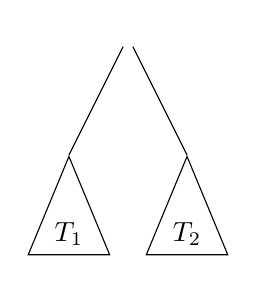
\begin{tikzpicture}
\usetikzlibrary{shapes.geometric}
\node {} [child anchor = apex]
child {node[draw, thin, isosceles triangle, anchor = apex, shape border rotate = 90]{$T_1$}}
child {node[draw, thin, isosceles triangle, anchor = apex, shape border rotate = 90]{$T_2$}};
\end{tikzpicture}

  \caption{Constructing a tree from subtrees}
  \label{fig:BinTreeConstruction}
\end{figure}
Also in addition to drawing pictures of binary trees, we can use a linear notation (something that  can we written 
in the midst of prose). 
If $T_1$ and $T_2$ are simple binary trees, we may denote the tree constructed by grafting $T_1$ on the left and $T_2$ on the right
as $(T_1\wedge T_2)$ (as in Figure \ref{fig:BinTreeConstruction}. Thus we define simple binary trees, and two operations
on them, as follows.

\begin{defn}
\emph{Simple binary trees} are defined inductively by
\[T \defeq \bullet \,\mid\, (T_1\wedge T_2)\]
The \emph{size} of a simple binary tree a natural number defined by the equations
\begin{align*}
  \sz(\bullet) &\defeq 0\\
  \sz(T_1\wedge T_2) &\defeq 1 + \sz(T_1) + \sz(T_2)
\end{align*}
The \emph{height} of a simply binary tree a natural number is defined
by the equations
\begin{align*}
  \hght(\bullet) &\defeq 0\\
  \hght(T_1\wedge T_2) &\defeq 1 + \max(\hght(T_1),\hght(T_2))
\end{align*}
where $\max(m,n)$ is the larger of the two numbers.
\end{defn}

These definitions suggest a relation between the size and height of a tree.
\ipadbreak

\begin{lemma}
For any simple binary tree $T$,  \[\hght(T)\leq \sz(T) < 2^{\hght(T)}.\]

\begin{proof}
To prove this by \emph{structural induction}, we must prove it for the basis ($\bullet$)
and that if it is true for some $T_1$ and $T_2$, then it is true for $(T_1\wedge T_2)$.
\begin{itemize}
\item{}[Basis] $\hght(\bullet) = 0$, $\sz(\bullet) = 0$ 
and $2^{\hght(\bullet)} = 1$. So the claim is true for $\bullet$.
\item{}[Inductive Hypothesis] Suppose the inequalities holds for some $T_1$ and $T_2$.
\item{}[Inductive Step] We must prove the two inequalities for $T= (T_1\wedge T_2)$.
Without loss of generality, assume that $\hght(T_1)\leq \hght(T_2)$. That is, if 
this is not so, then we may swap $T_1$ for $T_2$ in the following. 
\begin{align*}
\hght(T) &= 1 + \max(\hght(T_1),\hght(T_2)) &&\text{[Definition of $\hght$]}\\
         &\leq 1 + \hght(T_1) + \hght(T_2)  &&\text{[Arithmetic]}\\
         &\leq  1 + \sz(T_1) + \sz(T_2) &&\text{[Inductive Hypothesis]}\\
         &= \sz(T) &&\text{[Definition of $\sz$]}
       \end{align*}
And
\begin{align*}
\sz(T) &= 1 +\sz(T_1) + \sz(T_2)&&\text{[Definition of $\sz$]}\\
       &\leq 1 + 2^{\hght(T_1)} - 1) + (2^{\hght(T_2)} - 1)&&\text{[Inductive Hypothesis]}\\
       &\leq 2\cdot 2^{\hght(T_2)} - 1&&\text{[Assumption that $\hght(T_1)\leq \hght(T_2)$]}\\
       &= 2^{\hght(T_2)+1} - 1 &&\text{[Arithmetic]}\\
       &= 2^{\hght(T)} - 1 &&\text{[Definition of $\hght$]}
     \end{align*}
So $\sz(T) < 2^{\hght(T)}$
   \end{itemize}
 \end{proof}  
\end{lemma}

\ipadbreak

\begin{exercises}
  \item Calculate the height and size of the following simple binary trees.
    \begin{enumerate}
    \item $(\bullet\wedge\bullet)$
    \item $(\bullet\wedge (\bullet\wedge\bullet))$
    \item $((\bullet\wedge\bullet)\wedge(\bullet\wedge(\bullet\wedge\bullet)))$
    \item $((\bullet\wedge(\bullet\wedge\bullet))\wedge ((\bullet\wedge\bullet)\wedge(\bullet\wedge(\bullet\wedge\bullet))))$
    \end{enumerate}
   \item Draw diagrams (similar to those in Figure \ref{fig:BinTree}) for the following
   simple binary trees.
   \begin{enumerate}
   \item $((\bullet \wedge \bullet)\wedge(\bullet\wedge\bullet))$
   \item $(((\bullet\wedge\bullet)\wedge\bullet)\wedge ((\bullet\wedge\bullet)\wedge(\bullet\wedge(\bullet\wedge\bullet))))$
   \end{enumerate}
   \item For each of the following diagrams, write the expression using $\bullet$ and $\wedge$
    defining the same tree.
\begin{multicols}{2}
    \begin{enumerate}
    \item 
\begin{tikzpicture}
\node {}
child {node {$\bullet$}}
child {node  {}
       child {node {$\bullet$}}
       child {node {$\bullet$}}
      };
\end{tikzpicture}

 \item 

\begin{tikzpicture}
[level/.style={sibling distance = 2cm/#1, level distance = 1.5cm}]
\node {}
child {node  {}
       child {node {$\bullet$}}
       child {node {$\bullet$}}
      }
child {node  {}
       child {node {$\bullet$}}
       child {node {$\bullet$}}
      };
\end{tikzpicture}

\item

\begin{tikzpicture}
\node {}
child {node  {}
       child {node {} 
              child {node {$\bullet$}}
              child {node {$\bullet$}}}
       child {node {$\bullet$}}
      }
child {node  {$\bullet$}};
\end{tikzpicture}

    \end{enumerate}
  \end{multicols}
\end{exercises}


\begin{exercise}
\newcommand{\unit}{\mathord{\textbf{u}}}
\newcommand{\B}{\mathord{\textbf{B}}}
\newcommand{\C}{\mathord{\textbf{C}}}
\newcommand{\denotation}{\mathord{\textsf{val}}}

A \emph{widget} is defined inductively by
\[M \defeq \unit \mid M\B \,\mid\, M\C\]

For two widgets $M$ and $N$, their
\emph{merge} is a widget, denoted by $M\oplus N$, defined by
\begin{align*}
\unit \oplus \unit &\defeq \unit\B\\
\unit \oplus N\B &\defeq N\C\\
\unit \oplus N\C &\defeq (\unit \oplus N)\B\\ 
M\B \oplus \unit &\defeq M\C\\
M\B \oplus N\B &\defeq (M\oplus N)\B\\
M\B \oplus N\C &\defeq (M\oplus N)\C\\
M\C \oplus \unit &\defeq  (M\oplus \unit)\B\\
M\C \oplus N\B&\defeq (M\oplus N)\C\\
M\C \oplus N\C&\defeq ((M\oplus N) \oplus \unit)\B
\end{align*} 

For a widget $M$, its \emph{value} is a natural number, denoted by
$\llbracket M\rrbracket$, defined by
\begin{align*}
  \llbracket\unit\rrbracket &\defeq 1\\
  \llbracket M\B\rrbracket &\defeq 2\cdot \llbracket M\rrbracket\\
  \llbracket M\C\rrbracket &\defeq 2\cdot \llbracket M\rrbracket + 1
\end{align*}

Show that $\llbracket M\rrbracket + \llbracket N\rrbracket = \llbracket M\oplus N\rrbracket$ for any two
widgets $M$ and $N$.
\end{exercise}
}
%%% Local Variables: 
%%% mode: latex
%%% TeX-master: "MainText"
%%% End: 

%\chapter{Other Number Systems}

Discrete Mathematics is not only concerned with natural numbers. Integers, rational numbers, real numbers and even, on a few occasions, complex numbers, all play their roles. In this lecture, we discuss, with much less formality, integers and rational numbers, leaving real and complex numbers to a courses on analysis.

\begin{goals}
\begin{goal}{Lecture}
\item Introduce the standard notation for these number systems.
\item Discuss briefly the extensions of arithmetic to integers, rationals.
\item Wave hands and mumble unconvincingly about real and complex numbers.
\end{goal}

\begin{goal}{Study}
\item Learn the meanings of the symbols for standard number systems.
\item Prove some simple facts about arithmetic on integers and rational numbers.
\end{goal}
\end{goals}

\section{Integers}

Our intention here is to give a general overview of the integers in light of our detailed study of natural numbers.
Though we could, we will not go into the same level of detail.

Integers, we understand, include the natural numbers but also include negatives. They constitute the simplest possible extension of the natural numbers in such a way so that for any integers $a$ and $b$, there is a solution of the equation $a = b + x$.  
So the fundamental structure of integers is that (a) the natural numbers are integers and (b) addition on integers is invertible, i.e., subtraction works correctly.

\begin{postulate}\label{post:IntSignature}
The integers have the following basic structure.

\begin{itemize}
\item Every natural number is an integer. For this discussion, we will use letters $a$, $b$, $c$, \ldots for integers,
and $m$, $n$, \ldots for natural numbers.
To emphasize when a natural number $m$ plays the role of an integer we write ${}^+m$.
\item For every two integers, $a$ and $b$, there is a \emph{sum} and a \emph{difference}, denoted by $a+b$ and $a-b$. 
\end{itemize}
\end{postulate}

We must insist that addition on integers behaves as we should expect. 
\begin{postulate}\label{post:IntAddition}
For natural numbers $m$ and $n$,
\[{}^+m + {}^+n = {}^+(m+n).\]
That is, adding $m$ and $n$ \emph{as integers} is the same as adding them \emph{as natural numbers}.

Furthermore, addition on integers is associative and commutative, and $a + {}^+0 = a$ for all integers $a$.
\end{postulate}

Next, sum and difference are related.

\begin{postulate}\label{post:IntSubtraction}
For any integers $a$, $b$ and $c$, 
\[a = b + c\quad\text{if and only if}\quad a - b = c\]
\end{postulate}

Finally, we require minimality.

\begin{postulate}\label{post:IntInduction}
  No integers can be removed without violating Postulate \ref{post:IntSignature}.
\end{postulate}

We do not go through the details, but these axioms determine the structure of the integers similar to the way our earlier axioms determine the structure of the natural numbers. 
Moreover, all the familiar laws of addition and subtraction follow.
We illustrate with two simple laws. 
As usual, we can abbreviate ${}^+0-a$ by $-a$.

\begin{lem}\label{lem:IntAdditiveInverse}
For any integer $a$, ${}^+0= a + -a$.

\begin{proof}
  Since ${}^+0-a = {}^+0-a$ (trivially), Postulate \ref{post:IntSubtraction} yields ${}^+0 = a + ({}^+0-a) = a + (-a)$.
\end{proof}
\end{lem}

\begin{lem}\label{lem:IntAddSub}
  For integers $a$ and $b$, $a-b = a + (-b)$.

  \begin{proof}
    $a = a + {}^+0 = a + (-b + b) = b + (a+(-b))$ by the basic laws of addition (identity, commutativity and associativity)
and the previous lemma. So by Postulate \ref{post:IntSubtraction}, $a-b = a + (-b)$.
  \end{proof}
\end{lem}

In the axiomatization of integers, we did not mention multiplication. This is because multiplication is definable from addition. But we need an aditional fact.

Say that an integer $a$ is ``simple'' if either $a={}^+m$ or $-a = {}^+m$ for some natural number $m$. 

\begin{lem}
	Every integer is simple.
	
	\begin{proof}
		Exercise
	\end{proof}
\end{lem}

\begin{defn}
For any two integers $a$ and $b$, the \emph{product} $a\cdot b$ defined as follows:
\begin{align*}
	a\cdot {}^+0 &= {}^+0\\
	a\cdot {}^+(k^\nxt) &= a + a\cdot {}^+k\\
	a\cdot (-{}^+m) &= -(a\cdot {}^+m)
\end{align*}
\begin{itemize}
\item If $a\cdot {}^+0- ${}^+m\cdot {}^+n = {}^+(m\cdot n)$ for natural numbers $m$ and $n$;
\item Multiplication is associative and commutative, and $a\cdot {}^+1 = a$ for all integers $a$;
\item Multiplication distributes over addition.  
\end{itemize}
\end{defn}

These requirements are enough to ensure that multiplication is the operation we expect it to be.
We will not verify that fact, but it involves an inductive argument similar to the arguments that we saw in previous lectures.

\begin{exer}
	\begin{exercise}
\item Using only the axioms for integers, the foregoing two lemmas and the definition of multiplication, prove the following (remember
that $-a$ abbreviates ${}^+0 - a$). 
You should prove these in the order presented here, as later exercises may depend on earlier ones.
\begin{enumerate}
\item Show that $+$ is cancellative, not just on natural numbers, but on all integers: $a + c = b + c$ implies $a = b$.
\item Show that $a-b = -(b-a)$
\item Show that $(a+b) - c = a + (b-c)$
\item Show that $a-(b+c) = (a-b)-c$
\item Show that $-(-a) = a$
\item Show that ${}^+0\cdot a = {}^+0$
\item Show that $-a\cdot -b = a\cdot b$
\end{enumerate}
\item Show that every integer is simple, using only the postulates given here.

Hint: First observe that, trivially, every integer of the form ${}^+m$ is simple.
This acts as the basis for an inductive proof. 
Now suppose $a$ and $b$ are simple (the inductive hypothesis).
Show that both $a+b$ and $a-b$ are simple (the inductive step).
Since the integers are minimal for including the natural numbers and being closed under $+$ and $-$, this shows that all integers are simple.
\end{exercise}
\end{exer}

\section{Rational Numbers}

Rational numbers, roughly, are minimal with respect to the integers and multiplication, similar to 
integers being minimal with respect to natural numbers and addition. Care must be taken, however, because $0\cdot a = 0\cdot b$
does not tell us anything about $a$ and $b$. This means that ``division by $0$'' can not make sense.  

\begin{postulate}\label{post:RatSignature}
The rational numbers have the following basic structure.
\begin{itemize}
\item Every integer is a rational number. For this discussion, to emphasize when an integer $a$ plays the
role of a rational number, we write $\frac{a}{1}$. 
\item For every two rational numbers $p$ and $q$, there is a \emph{product}, denoted by $p\cdot q$.
Moreover, if $q\neq \frac{0}{1}$, then there is a \emph{quotient}, denoted by $p/q$.
\end{itemize}
\end{postulate}

In analogy with integers, where addition and subtraction are the main operations, we insist that
multiplication behaves correctly. 

\begin{postulate}\label{post:RatMultiplication}
For integers $a$ and $b$,
\[\frac{a}1 \cdot \frac{b}1 = \frac{ab}1\]
That is, multiplying integers $a$ and $b$ \emph{as rational numbers} is the same as multiplying them \emph{as integers}.

Furthermore, multiplication is associative and commutative, and $p \cdot \frac{1}{1} = p$ for all rational numbers $p$.
\end{postulate}

Again, continuing the analogy with integers, multiplication and division must cooperate.
\begin{postulate}\label{post:rationaldivision}
For any rationals $p$, $q$ and $r$,
if $q\neq \frac{0}1$, then 
\[p= q \cdot r\quad\text{if and only if}\quad p/q = r\]
\end{postulate}

Finally, we require minimality.

\begin{postulate}\label{post:RationalInduction}
  No rational numbers can be removed without violating Postulate \ref{post:RatSignature}.
\end{postulate}

Like the axioms for integers, these axioms completely determine the rational numbers along with multiplication and division. 
To extend addition and subtraction to the rational numbers we can require the following.

\begin{defn}
For any two rational numbers $p$ and $q$, their \emph{sum} and \emph{difference}, denoted by $p+q$ and $p-q$, are rational numbers
satisfying:
\begin{itemize}
\item  $\frac{a}{1} + \frac{b}{1} = \frac{a+b}{1}$ for integers $a$ and $b$. 
\item Addition is associative and commutative, and $p + \frac{{}^+0}1 = p$ for all rational numbers $p$;
\item $p = q + r$ if and only if $p - q = r$ for all rational numbers $p$, $q$ and $r$;
\item Multiplication distributes over addition.
\end{itemize}
\end{defn}

These requirements are enough to ensure that addition is the operation we expect
it to be. 

Now suppose $a$ is an integer and $m$ is a positive natural number. Then we
can write $\frac{a}m$ as an abbreviation of $\frac{a}{1} / \frac{{}^+m}1$. This is
the usual \emph{fraction} notation for rational numbers.
For a non-zero rational number $p$, we also usually write $p^{-1}$ to abbreviate 
$\frac{{}^+1}{1}/ p$.

\begin{exer}
\begin{exercise}
\item Using the proof of Lemma \ref{lem:IntAdditiveInverse} as a prototype, show that if $p\neq \frac{{}^+0}{1}$,
then $p\cdot p^{-1} = \frac{{}^+1}{1}$. 
\item Using the proof of Lemma \ref{lem:IntAddSub} as a prototype, show that $p/ q = p\cdot q^{-1}$
when $q\neq \frac{{}^+0}{1}$.
\item Just using our axioms and the fraction notation (and the previous two exercises),
show that $\frac{4}{6} = \frac{2}{3}$.
\end{exercise}
\end{exer}

\section{Real and Complex Numbers}

We will not deal with rigorous characterizations of the real numbers and complex numbers in this course. 
A first course in real analysis is the appropriate place for such considerations. 
We simply take for granted that $\RR$ constitutes a suitable
extension of $\QQ$ to account for \emph{limits} (the mathematics you know from calculus). Likewise, $\CC$
constitutes a suitable extension of $\RR$ to account for 
algebraic closure (all polynomials having roots). The main things to know are that every rational number is real,
every real number is complex, and arithmetic operations behave as they should for real and complex numbers.

\begin{exer}
\begin{exercise}
  \item Relax. Take a walk.
\end{exercise}
\end{exer}

% 1
%\input{PythonPrimer.tex}
%\input{SumAndProduct.tex}

% 1
%\input{Numerals.tex}

% 2
%\chapter{Ordering the Natural Numbers by Addition}

We have used the ordering of numbers informally without much comment
because $\leq$ has its obvious meaning. In this lecture 
we exploit the fact that $\leq$ on the natural numbers is defined by addition, setting the stage for an
analogous concept defined by multiplication. The multiplicative
analogue of ``$m$ is less than or equal $n$'' is ``$m$ divides $n$''.

\begin{goals}
\begin{goal}{Lecture}
\item Introduce a formal definition of $\leq$ on natural numbers, and discuss simple facts about order
%\item Introduce formal definitions $\min$ and $\max$ as dual concepts
\item Review basic laws involving $\min$ and $\max$.
\item Introduce Strong Induction and the Principle of Well-foundedness as alternatives to Simple Induction.
\end{goal}

\begin{goal}{Study}
\item Prove basic facts about $\leq$, $\min$ and $\max$.
\item Commit to memory the concepts of reflexivity, transitivity, anti-symmetry and linearity.
\item Practice using Strong Induction.
\end{goal}
\end{goals}


\section{Less or Equal}

For the natural numbers, $\leq$ has a particularly simple definition.

\begin{defn}
  For natural numbers $n$ and $m$, say that \emph{$m$ is less than or equal to $n$} (written $m\leq n$)
  if and only if there is a
  natural number $d$ so that $m+d = n$.  [I've used the letter $d$
  because $d$ is the \emph{difference} of $m$ from $n$.]
  
  Also, say that \newterm{$m$ is (strictly) less than $n$} if and only if there is a natural number $d$ so that $m + d^\nxt = n$.
\end{defn}

All of the usual properties of $\leq$ for natural numbers follow
easily from this definition using only the laws of
addition. The important properties have names.

\begin{laws} 
\begin{description}
	\item[Reflexivity] $\leq$ is \emph{reflexive}: $m\leq
m$ is true for any $m$. This is simply because because $m + 0 =
m$. 
    \item[Transitivity] $\leq$ is \emph{transitive}: if $m\leq
n$ and $n\leq p$, then $m\leq p$. Transitivity follows from the law of
associativity for addition (you will prove this as an exercise).
    \item[Anti-symmetry] $\leq$ is \emph{anti-symmetric}: if $m\leq n$ and $n\leq m$, then
	$m=n$. This follows from cancellativity and positivity (another exercise).
	\item[Linearity] $\leq$ is \emph{linear}: for any $m$ and $n$, either $m\leq n$ or $n\leq m$. This requires a separate proof using induction, dealt with below.
\end{description}
\end{laws} 

Clearly, $\leq$ is also meaningful for integers, rational numbers and real numbers, and is still reflexive, transitive and anti-symmetric and linear for them.
For our purposes, though, the interesting features are already present in the natural numbers.
For one thing, if $m+d = n$ and $m+e = n$ then $d=e$ (why?). This tells us that $m\leq n$ can only be true for one reason.

\ipadbreak

\begin{exer}
	In the following you will use the Laws of Arithmetic from Lecture \ref{lec:ArithmeticLaws} to prove the basic facts about $\leq$.
	\begin{exercise} 
    \item Show that $\leq$ is transitive by the following steps.
    \begin{enumerate}
    \item Assume that $m\leq n$. By definition, there is some $d_0$ so
      that $m+d_0 = n$
    \item Assume that $n\leq p$. Write out what this means. ``By
      definition, there is some \ldots''
    \item Now find an $e$ so that $m+e = p$.
    \item Write out the conclusion.
    \end{enumerate}

    \item Show that $\leq$ is anti-symmetric by the following steps.
    \begin{enumerate}
    \item Assume $m\leq n$. Write out what this means: ``There is some
      $d_0$ so that \ldots.''
    \item Assume $n\leq m$. Write out what this means. ``There is some
      $d_1$ so that \ldots.''
    \item Show that $d_0 + d_1 = 0$. [Think about using
      cancellativity.]
    \item Conclude that $d_0 = 0$. [Which law justifies this?]
    \item Conclude that $m = n$.
    \end{enumerate}
	\end{exercise}
\end{exer}

As we mentioned, $\leq$ is \emph{linear}, meaning
that for any $m$ and $n$, either $m\leq n$ or $n\leq m$. A proof of
this is not terribly difficult, but is more subtle than transitivity and anti-symmetry.

\begin{lem}
  \emph{$\leq$ is linear.}

  \begin{proof}
  	Note that we defined linearity in terms of $\leq$, but it is equivalent to saying that for any $m$ and $n$, either $m<n$ )or $n\leq m$. After all, if $m<n$ then $m\leq n$. And if $m\leq n$, then either $m=n$ and hence $n\leq n$, or $m<n$.  
    A proof is by induction on $m$.
    \begin{itemize}
    \item{}[Basis] $0 + n = n$ is always true. So $0\leq n$.
    \item{}[Inductive Hypothesis] Suppose that for some $k$, it
      is the case that either
      $k\leq n$ or $n\leq k$ (but we do not know which comparison is true).
    \item{}[Inductive Step] We must show that either $k^\nxt \leq n$ or
      $n\leq k^\nxt$.  According to the Inductive Hypothesis, there
      are two cases to consider. Either $k\leq n$ or $n\leq k$. We take them in reverse.
      \begin{enumerate}
      	\item Suppose $n\leq k$. 
	      	Then obviously $n\leq k^\nxt$ (meaning, it is so obvious that we do not bother to fill in the details).
		    \item Suppose $k< n$. So for some $d$, $k+d^\nxt =n$. Hence $k^\nxt+d=n$. if $d=0$, then $k^nxt = n$, so $n\leq k^\nxt$. Otherwise, $k^\nxt < n$.
      \end{enumerate}
    \end{itemize}
  \end{proof}
\end{lem}

\begin{exer}
	The following proofs should require you only to refer to the definition of $\leq$ and to the basic Laws of Arithmetic.
	\begin{exercise}
		\item Prove that addition is \newterm{monotonic} with respect to $\leq$. This means that $m\leq n$ implies $m+p\leq n+p$ for all natural numbers $m$, $n$ and $p$.
		\item Prove that addition is \newterm{order reflectiing} with respect to $\leq$. This means that if $m+p\leq n+p$, then $m\leq n$.
	\end{exercise}
\end{exer}

\section{Other Forms of Induction}

Using $\leq$, we can formulate a more flexible method of proof by induction.

Suppose we wish to prove that all natural numbers are \emph{outgrabe}.
Again this is nonsense, but let's try anyway. We prove the basis with no trouble; formulate the Inductive Hypothesis; get stuck on the Inductive Step.
Here is a simple idea that can help. 
Define a \emph{hypergrabe} number to be a natural number $k$ so that for every $j<k$, $j$ is outgrabe.
In other words, $k$ does not necessarily have the property we really care about, but all the numbers below it do.
Now suppose every natural number is outgrabe.
Then clearly, every natural number is also hypergrabe.
Likewise, if every natural number is hypergrabe, then every natural number is outgrabe.
So proving either property by induction will suffice to prove the other.
A proof by simple induction that all natural numbers are hypergrabe amounts to this:
\begin{itemize}
	\item{}[Basis] Show that every natural number $j<0$ is outgrabe. But since there are no such numbers, this is trivially true no matter what outgrabe happens to mean.
	\item{}[Inductive Hypothesis] Suppose that $k$ is hypergrabe for some $k$.
	That is, suppose that for all $j<k$, $j$ is outgrabe.
	\item{}[Inductive Step] Prove that $k^\nxt$ is hypergrabe.
	By the Inductive Hypothesis, all $j<k$ are outgrabe.
	So to prove that every $j<k^\nxt$ is outgrabe just amounts to
  proving it for $k$.
  So the Inductive Step (for proving that $k^\nxt$ is hypergrabe) amounts to proving that $k$ is outgrabe. 
\end{itemize}

This can now be reformulated without mentioning \emph{hypergrabe} at
all.  
The Basis is not needed, because it is true automatically.  
The Inductive Hypothesis can be reformulated as supposing that for all $j<k$, $j$ is outgrabe. 
The proof of the Inductive Step amounts to proving that $k$ is outgrabe.

This leads to a formulation of induction that is typically called
\emph{Strong Induction}, even though it is not really any stronger (i.e., it is not able to prove more facts).
A proof of property $P$ by Strong Induction has the outline:
\begin{itemize}
\item{}[Strong Inductive Hypothesis] Suppose that $P(j)$ is true for all $j<k$.
\item{}[Strong Inductive Step] Prove that $P(k)$ is true.
\end{itemize}

Exercises involving strong inductive proofs are not easy to come by right now.
We will see a very important example when we prove that every positive natural number can be factored into primes.

\begin{example}
Here is an example that uses strong induction to prove something. Define Fibonnacci number $f_n$ by the equations
\begin{align*}
  f_0 &= 0\\
  f_1 &= 1\\
  f_{n+2} &= f_{n+1} + f_n & \text{for any $n$}
\end{align*}
We claim that for all $n$, $2f_n \leq f_{n+2}$.

\begin{itemize}
\item{}[Strong Inductive Hypothesis] Suppose that for all $j<k$, $2f_j \leq f_{j+2}$.
\item{}[Strong Inductive Step]. We need to show that the claim also holds 
for $k$.
In case $k=0$, this is obviously true because $2f_0 = 0$. In case
$k=1$, it is also obviously true because $2f_1 = 2 = f_3$. 
In all other cases $k=i+2$ for some $i$. So 
\begin{align*}
2f_k  &= 2f_i + 2f_{i+1}&&\text{[By definition of $f$ and distributivity]}\\ 
      &\leq f_{i+2} + f_{i+3}&&\text{[By Inductive Hypothesis]}\\
      &= f_k + f_{k+1}&&\text{[$i+2=k$]}\\
      &= f_{k+2}&&\text{[By definition of $f$]}
    \end{align*}
\end{itemize}
\end{example}

We close this section with another method for using induction that is sometimes useful. 

\begin{lemma}\label{lem:N-well-ordered}
Suppose $P(-)$ is a property that makes sense for natural numbers. Suppose, furthermore, that $P(m)$ is
true for some $m$. Then there is a smallest $m$ for which $P(m)$ is true. That is, there is
a natural number $m_0$ so that $P(m_0)$ and so that $P(n)$ implies $m_0\leq n$. 
\begin{proof}
  Suppose $P(-)$ is a property that makes sense for natural numbers and that there is no
minimal $m$ for which $P(m)$ is true. We will show that $P(m)$ is false for all $m$ by strong induction.
\begin{itemize}
\item{}[Strong Inductive Hypothesis] Assume that $P(j)$ is false for all $j<k$.
\item{}[Inductive Step] We must show that $P(k)$ is also false. Suppose $P(k)$
were true. By the strong inductive hypothesis, $P(j)$ is false for all $j<k$. So $k$ would be the smallest
natural number for which $P(k)$ is true. This contradicts the assumption that there is no minimal value
for which $P(m)$ is true. So $P(k)$ must not be true.
\end{itemize}
\end{proof}
\end{lemma}

\begin{exer}
	\begin{exercise}
		\item Define the ``tribonacci'' numbers as follows:
		\begin{align*}
			t_0 &= 0\\
			t_1 &= 1\\
			t_2 &= 2\\
			t_{n+3}& = t_{n+2} + t_{n+1} + t_n & \text{for each $n$} 
		\end{align*}
		Prove by strong induction that $t_n < 2^{n-1}$ is true for all natural numbers $n$. [Recall that $2^{-1} = \frac{1}{2}$.]
		\item Prove that $n^3<3^n$ for all natural numbers $n$.
	\end{exercise}
\end{exer}

\section{Minimum and Maximum}

The minimum of two numbers $m$ and $n$ is, of course, the smaller of the two. 
We write $\min(m,n)$ for this. The maximum is written as $\max(m,n)$. To make this
precise, we can write a formal definition.

\begin{defn}
  For natural numbers $m$ and $n$, $\min(m,n)$ is a natural number satisfying:
  \begin{itemize}
  \item $\min(m,n)\leq m$ and $\min(m,n)\leq n$;
  \item for any natural number $p$, if $p\leq m$ and $p\leq n$, then $p\leq \min(m,n)$.
  \end{itemize}

Also, $\max(m,n)$ is defined \emph{dually}. For natural numbers $m$ and $n$, $\max(m,n)$ is a natural number satisfying:
\begin{itemize}
	\item $m\leq \max(m,n)$ and $n\leq \max(m,n)$;
	\item for any natural number $p$, if $m\leq p$ and $n\leq p$, then $\max(m,n)\leq p$.
\end{itemize}
\end{defn}


Both $\min$ and $\max$ are characterized by what we may call an ``adjoint situation''.
\begin{align*}
  p\leq \min(m,n) &\iff \text{$p\leq m$ and $p\leq n$}\\
  \max(m,n) \leq p&\iff \text{$m\leq p$ and $n\leq p$}
\end{align*}
This shows that comparing $p$ to two numbers on the right is the same as comparing $p$ to their minimum on the right; and similarly for comparison on the left and maximum.
We say that $\min(m,n)$ is the \emph{greatest lower bound} of $m$ and $n$ and that $\max(m,n)$ is the \emph{least upper bound} of $m$ and $n$. 

Some simple facts about $\min$ and $\max$ derive directly from this characterization by adjointness.
The two operations, $\min$ and $\max$, have many useful properties,
all of which can be proved using the above characterizations plus some facts about addition.

In particular, together with addition,  $\min$ and $\max$ make the natural numbers into something called a \emph{distributive lattice ordered monoid}.
Basically, this means that addition together with $\min$ and $\max$ cooperate in specific ways that are akin to the basic laws of arithmetic.
The most useful laws having to do with $\min$ and $\max$ are:


\begin{laws}
For all natural numbers $m$, $n$ and $p$:
	\begin{description} 
\item[Commutativity]
  \begin{align*}
    \min(m,n) &= \min(n,m)
    & \max(m,n) &= \max(n,m)\\
  \end{align*}
\item[Associativity]
  \begin{align*}
    \min(\min(m,n),p) &= \min(m,\min(n,p)) & \max(\max(m,n),p) &=
    \max(m,\max(n,p))
  \end{align*}
\item[Idempotency]
  \begin{align*}
    \min(m,m) &= m & \max(m,m) = m\\
  \end{align*}
\item[Absorption]
  \begin{align*}
    \min(m,\max(n,m)) &= m &\max(m,\min(n,m)) &= m
  \end{align*}
\item[Distributivity]
  \begin{align*}
    m + \min(n,p) &= \min(m+n,m+p) & m + \max(n,p) &= \max(m+n,m+p)\\
    \max(m,\min(n,p)) &= \min(\max(m,n),\max(m,p)) & \min(m,\max(n,p)
    &= \max(\min(m,n),\min(m,p))
  \end{align*}
\item[Modularity]
  \begin{align*}
    m + n &= \min(m,n) + \max(m,n)
  \end{align*}
  \end{description}
\end{laws}

We will not prove most of these as they follow easily from arithmetic laws. But the most subtle is worth looking at.

\begin{lemma}
$m + \min(n,p) = \min(m+n, m+p)$ for all $m,n,p\in\NN$.
\begin{proof}
By definition, $\min(n,p)\leq n$. Because addition is monotonic, $m+\min(n,p) \leq m+n$. Likewise $m+\min(n,p)\leq m+p$. So $m+\min(n,p)\leq \min(m+n,m+p)$.

So to complete the proof, we must show that $\min(m+n,m+p)\leq m+\min(n,p)$. 
Suppose $k\leq \min(m+n,m+p)$. Then if $k\leq m$, then $k\leq m+\min(n,p)$ obviously.
Otherwise, $m\leq k$ by Linearity. So $m+d = k$ for some $d$. Hence $m+d \leq m+n$ and $m+d \leq m+p$. Since $\leq$ is order reflecting, $d\leq \min(n,p)$. Consequently, $k=m+d \leq m+\min(n,p)$. We have thus shown that $k\leq \min(m+n,m+p)$ implies $k\leq m+\min(n,p)$. 
In particular, this applies to $\min(m+n,m+p)$.
\end{proof}
\end{lemma}

\begin{exer}
\begin{exercise}
	\item Calculate the following values. Show work.
  \begin{enumerate}
  \item $\min(5,\min(4,6))$
  \item $\min(5, \max(4,6))$
  \item $\min(340, \max(234, 340))$
  \item $\min(5,\max(3,\min(\max(1,2),7)))$
  \item $\min(5+\max(4 + \min(3 + \max(7,8), 3+ \min(7,8)), 6), 7)$
  \end{enumerate}
  \item Prove that $\min$ distributes over $\max$.
\end{exercise}
\end{exer}

\chapter{Divisibility}

\begin{goals}
	\begin{goal}{Lecture}
		\item Develop the analogue of $\leq$ defined by multiplication instead of by addition.
		\item Illustrate the value of the analogy to prove useful properties of divisibility.
		\item Introduce general division for natural numbers.
	\end{goal}
	
	\begin{goal}{Study}
		\item Demonstrate competence in determining divisibility and division facts.
	\end{goal}{Study}
\end{goals}

For natural numbers, $m\leq n$ \emph{means} that $m+d = n$ for some $d$.
Since multiplication satisfies many of the same laws (it is commutative, associative, etc.), a similar definition is possible in terms of multiplication.

\begin{defn}
  For natural numbers $m$ and $n$, say that \newterm{$m$ divides $n$}, if and only if $m\cdot q = n$ for some natural
  number $q$.
  We write $m\mid n$ when $m$ divides $n$.
\end{defn}

We have an analogy between ``$m$ is less than  or equal to $n$'' and ``$m$ divides $n$.'' 
The difference is precisely that the former is defined by addition and the latter by multiplication.
This is useful because we can sometimes transfer a fact about $\leq$ to a fact about $\mid$ simply by noticing that they both depend on analogous laws of arithmetic.

For example, the relation $\leq$ is reflexive \emph{because} $0$ is the identity for addition.
The relation $\mid$ is reflexive because $1$ is the identity for multiplication.
Likewise, $\leq$ is transitive \emph{because} addition is associative; 
so $\mid$ is transitive because multiplication is associative. 

Anti-symmtry is also true, but a proof hints at why our analogy is not perfect. 
Recall that we proved that $m\leq n$ and $n\leq m$ implies $m=n$. using cancellativity of addition.
But multiplication is only cancellative for non-zeros.
That is, $m\cdot p = n\cdot p$ implies $m=n$ only when $p\neq 0$. 
This means that we need to treat $0$ as a special case. 
Suppose $m\cdot q = n$ and $n\cdot r = m$. If $m=0$, then obviously $n=0$.
So $m=n$.
If $m\neq 0$, then $m\cdot q\cdot r = m$ and $m\neq 0$.
So by cancellativity $q\cdot r = 1$, and so $q=1$. 
Hence $m = m\cdot 1 = n$.

The divisibility relation begins to be more interesting
when we realize that it is \emph{not} linear. For example,
$4$ does not divide $13$ and $13$ does not divide $4$.
Apparently, the structure of the natural numbers with respect
to $\mid$ is much more complicated that with respect to $\leq$.

Note that $1\mid m$ is true for any $m$, simply because $1\cdot m = m$.
And $m\mid 0$ is true for any $m$ because $m\cdot 0 = 0$.
So $1$ is ``at the bottom'' of the divisibility relation and $0$ is  ``at the top''. 
This may seem strange. Some people find it so irritating that they simply rule $0$ out of consideration, and declare that $0\mid 0$ is undefined. 
This is fine, but
I prefer to understand $0\mid 0$ to mean $0 \cdot q = 0$ for \emph{some $q$}.

Figure \ref{fig:Divisibility} shows a fragment of the natural numbers with respect to divisibility. 

\ipadbreak
 
\usetikzlibrary{3d}
\newcommand{\xangle}{19}
\newcommand{\yangle}{139}
\newcommand{\zangle}{90}
\newcommand{\xlength}{3}
\newcommand{\ylength}{2.5}
\newcommand{\zlength}{1.4}
\newcommand{\dimension}{3}% actually dimension-1
\pgfmathsetmacro{\xx}{\xlength*cos(\xangle)}
\pgfmathsetmacro{\xy}{\xlength*sin(\xangle)}
\pgfmathsetmacro{\yx}{\ylength*cos(\yangle)}
\pgfmathsetmacro{\yy}{\ylength*sin(\yangle)}
\pgfmathsetmacro{\zx}{\zlength*cos(\zangle)}
\pgfmathsetmacro{\zy}{\zlength*sin(\zangle)}
\begin{figure}[ht]\label{fig:Divisibility}
\centering
\begin{tikzpicture}
[   x={(\xx cm,\xy cm)},
    y={(\yx cm,\yy cm)},
    z={(\zx cm,\zy cm)},
    scale=0.75
]
\foreach \a in {0,...,\dimension}
{   \foreach \b in {0,...,\dimension}
    {   \pgfmathsetmacro{\c}{100-\a*7-\b*7}
        \draw[canvas is xy plane at z=\a, black!\c] (\b,0) -- (\b,\dimension) (0,\b) -- (\dimension,\b);
        \draw[canvas is xz plane at y=\a, black!\c] (\b,0) -- (\b,\dimension) (0,\b) -- (\dimension,\b);
        \draw[canvas is yz plane at x=\a, black!\c] (\b,0) -- (\b,\dimension) (0,\b) -- (\dimension,\b);
    }
}
\foreach \a in {0,...,\dimension}
{   \foreach \b in {0,...,\dimension}
    {   \foreach \c in {0,...,\dimension}
        {  \pgfmathtruncatemacro{\d}{(5^\a)*(2^\b)*(3^\c)} 
           \node at (\a,\b,\c) [circle,draw, fill= white] {\tiny$\d$};
        }
    }
}

\node at (\dimension+1, \dimension+1, \dimension+1) [circle,draw, fill=white] {\tiny$0$};
\foreach \a in {0,...,\dimension} {
   \node at (\a, \dimension, \dimension+1) {$\vdots$};
}
\foreach \b in {0,...,\dimension} {
   \node at (\dimension, \b, \dimension+1) {$\vdots$};
}

\end{tikzpicture}
\caption{Part of the divisibility relation}
\end{figure}

\ipadbreak

\begin{exer}
    For each of the following pairs $(m,n)$ of natural numbers, determine whether or not $m\mid n$.
    \begin{exercise}
    \item $(4,202)$
    \item $(7, 49)$
    \item $(11, 1232)$
    \item $(9, 19384394)$
    \item $(n,6n)$
    \item $(26,65)$
    \end{exercise}
\end{exer}

Divisibility also makes sense for integers, but it is no longer anti-symmetric for a somewhat trivial reason.
For example, $5\mid -5$ and $-5\mid 5$, but obviously $5\neq -5$. In short, divisibility ignores the sign of an integer.
This is a good reason for us to concentrate our attention on natural numbers, bearing in mind that much of what we can say about divisibility is true for integers as well.

Before closing this section, we note additional facts about how $\mid$ interacts with arithmetic.

\begin{prop}
  \begin{enumerate}
    \item $m\mid n$ implies $m\mid np$
    \item $m\mid n$ and $m\mid p$ implies $m\mid (n+p)$
    \item $0<n<m$ implies $m\nmid pm+n$
    \item $m\mid n$ and $n>0$ implies $0< m\leq n$.
  \end{enumerate}

  \begin{proof}
  	\begin{enumerate}
    \item is true by associativity.
    \item is due to distributivity.
    \item can be proved by showing that $mq\neq pm + n$ for all $q$.
    We leave this as a voluntary exercise.
    \item uses (3). That is, suppose $m\mid n$ and $n>0$. 
    Then we can write this as $m \mid 0\cdot m + n$. Thus $0<m$.
    And according to (3), $0<n<m$ has to fail.
    Since $0<n$ holds by assumption, $m\leq n$.
    \end{enumerate}
  \end{proof}
\end{prop}

\section{Quotients and Remainders}

Without rational numbers, division still makes sense. 
We only need to account for the fact that sometimes numbers don't divide evenly.
To make this work properly, we can speak of a \emph{quotient} and \emph{remainder}. 
For example, dividing $23$ by $7$ results in a quotient of $3$ and a remainder of $2$. 
That is, $3\cdot 7 + 2 = 23$. 
Let us make this precise.

\begin{thm}[Natural Number Division]\label{thm:division}
	For any natural number $m$ and any positive natural number $n$, there is a unique pair of natural numbers $q$ and $r$ 
	satisfying
	\[m=qn + r\]
	and
	\[r < n\]
 
\begin{proof}
	First, we prove that if $q$ and $r$ satisfy the stated conditions, and so do $q'$ and $r'$, then $q=q'$ and $r=r'$.
	This will prove that there can be at most one pair of natural numbers satisfying the stated conditions.
	Suppose $qn+r = q'n+ r'$ and $r<n$ and $r'<n$. If $r<r$,
	then there is some positive $e$ so that $r+e=r'$. Hence $qn = q'n+e$. But this means that $n \mid q'n+e$. Clearly,
	$e<n$, so is
	impossible. Thus it can not be the case that $r<r'$. For the same reason, it can not be the case that $r'<r$. So $r=r'$. 
	
	Now we prove that there actually is a pair of numbers $q$ and $r$ satisfying the condtions. For this, we proceed by induction
	on $m$.
	\begin{itemize}
		\item{} [Basis] $0=0\cdot n = 0$. So $q=0$ and $r=0$ do the job.
		\item{} [Inductive hypothesis] Assume that for some $k$, natural numbers $p$ and $s$ exist for which $k=p\cdot n+s$ and $s<n$.
		\item{} [Inductive Step] We must find $q$ and $r$ so that $m^\nxt = q\cdot n+r$ and $r<n$. There are two cases: either $s^\nxt = n$
		or $s^\nxt < n$.
		Suppose $s^\nxt < n$. Then $m^\nxt = p\cdot n + s^\nxt$. So let $q=p$ and let $r=s^\nxt$. Suppose $s^\nxt = n$. Then $p\cdot n + s^\nxt = p^nx\cdot n + 0$. So let $q=p^\nxt$ and $r=0$.
	\end{itemize} 
\end{proof}
\end{thm}

This theorem indicates that division of natural numbers works, as long as we account for both the quotient and the remainder. It is useful to have notation for both of these.  So we will sometimes use the same notation for an integer divided by a positive natural number.

\begin{defn}
	For any integer $a$ and positive natural number $n$, let $a\ddiv n$ denote the \emph{quotient} and $a\drem n$ the \emph{remainder} of
	dividing $a$ by $n$. That is, $a\ddiv n$ and $a\drem n$ are the unique two integers so that
	\[a = (a\ddiv n)\cdot n + (a\drem n)\]
	and 
	\[0\leq a\drem n < n\] 
\end{defn}

The notation $\ddiv$ is borrowed from the programming langauge Python. It is intended to avoid confusion with real number division $x/y$.
Python, Java, C and many other languages use a percent sign for remainder,
but unfortunately, its precise meaning differs from langauge to language. The notation $\drem$ avoids this ambiguity.

\begin{exer}
\begin{exercise}
	\item Calculate the following:
		\begin{enumerate}
			\item $24\ddiv 7$
			\item $10000000\drem 10000001$
			\item $13\drem 8$
			\item $8\drem 5$
			\item $5\drem 3$
			\item $3\drem 2$
			\item $2\drem 1$
		\end{enumerate}
	\item Show that for any natural number $m$, any positive natural number $n$ and any positive natural number $p$, 
	it is the case that $pm\ddiv pn = m\ddiv n$ 
	and that $pm\drem pn = p(m\drem n)$.
\end{exercise}
\end{exer}

\chapter{Prime Numbers}

\begin{goals}
	\begin{goal}{Lecture}
		\item Prove the Fundamental Theorem of Arithmetic
		\item Prove that the prime numbers are unbounded in the natural numbers.
	\end{goal}
	
	\begin{goal}{Study}
		\item Demonstrate competence in prime factorization.
	\end{goal}
\end{goals}


We all know what a prime number is. It is a number that is not $1$ and has no non-trivial 
factors. One might ask why $1$ does not count as a prime number since it seems
like an arbitrary thing to exclude.
We settle that question here. The key insight (from an earlier lecture)
is that an \emph{empty product} is $1$.

Recall that the product of a list of natural numbers is defined inductively by
\begin{itemize}
\item $\prod [\,] = 1$
\item $\prod n:L = n \cdot \prod L$
\end{itemize}

\begin{defn}
  A \newterm{prime number} is a positive natural number $p$ so that for any list $L$ of natural numbers, if $p \mid \prod L$ holds, then $p \mid L_i$
holds for some $i<\len(L)$. In other words, if $p$ divides a product of natural numbers, it divides one of them.
\end{defn}

With this definition, $1$ is not prime for exactly the same reason that $6$
is not prime.
That is, $6$ is not prime because, for example, $6 \mid  \prod[2,3]$ but $6$ does not divide any item on the list $[2,3]$.
Likewise, $1 \mid  \prod [\,]$ but $1$ does not divide any item on the list $[\,]$ because there are no items on the empty list.
In contrast, $2$ is prime because if $2\mid\prod L$ with $L$ being a list of natural numbers, at least one of the items on the list must be even.
It is not hard to check that this definition of primality agrees with the more familiar one.

Our first task involving primes is to remind ourselves of the \emph{Fundamental Theorem of Arithmetic}, that every positive natural number factors uniquely into primes. 
We split the proof of this into two separate parts.

\begin{lem}\label{lem:prime-factorization}
  For any positive natural number $m$, there is a list $P$
consisting only of primes so that $m = \prod P$.

\begin{proof}
  Here we use strong induction. 
  \begin{itemize}
  \item{}[Strong Inductive Hypothesis] Assume that for some $k$, it is the case that for every $0<j<k$,
   there is a list of primes $P$ so that $j=\prod P$.
  \item{}[Strong Inductive Step] There are three cases to consider. Either $k=1$,
or $k = i\cdot j$ for some positive $i$ and $j$ strictly less than $k$, or neither of these holds.

Suppose $k = 1$. Then we let $P=[\,]$. This is
a (trivial) list of primes whose product is $k$.

  Suppose $k = i\cdot j$ where $i$ and $j$
  are both positive and strictly less than $k$. By the inductive hypothesis, 
  there are lists of primes $Q$ and $R$ so that $i=\prod Q$ and $j=\prod R$.
  Hence $k = \prod Q\cdot \prod R = \prod (Q\otimes R)$.

  Suppose $k$ is neither equal to $1$, nor equal to $i\cdot j$ for
any two natural numbers strictly less than $k$. Then $k$ itself is 
  prime. So $k = \prod [k]$. 

These are the only possible cases.
  \end{itemize}
\end{proof}
\end{lem}

The list of primes we constructed in the Lemma \ref{lem:prime-factorization} is
called a \newterm{prime factorization of $m$}. Generally, a composite has
more than one prime factorization for trivial reasons. For example, 
$[2,3]$ and $[3,2]$ both are prime factorizations of $6$. But the \emph{only} way 
two prime factorizations of the same number can differ is by the order 
in which the factors are listed. 
If we insist that our lists are sorted in increasing order, this ambiguity is avoided. 
That is, say $P$ is a \emph{sorted} list of natural numbers if $P_i\leq P_j$ whenever $i\leq j <\len(P)$.

\begin{lem}
For every positive natural number $m$, there is at most one sorted prime factorization of $m$.
\begin{proof}
Suppose $P$ and $Q$ are sorted prime factorizations of $m$. We need to show that they are equal.
We do this by structural induction on $P$. That is, we show that for all sorted lists of primes $Q$, 
if $\prod P = \prod Q$, then $P=Q$.
\begin{itemize}
\item{}[Basis] If $\prod [\,] = \prod Q$,
then $Q$ must also be the empty list because no non-empty list of primes has a
product of $1$.
\item{}[Inductive hypothesis] Assume that, for some fixed sorted list of primes $K$, it is the case that
for all sorted lists of primes $R$, if $\prod K = \prod R$, then $K=R$.
\item{}[Inductive Step] Suppose $\prod p:K = \prod Q$ where $p:K$ and $Q$ are
sorted lists of primes. Then $p\mid \prod Q$.
But $p$ is prime, so $p$ must appear somewhere in the list $Q$. There are two cases:
either $p$ is the initial item of $Q$, or not.

If $p$ is the initial element of $Q$, then we can write $Q = p:R$ for some list $R$.
By cancellativity, $\prod K = \prod R$. So by the inductive hypothesis, $K = R$.
So $p:K = Q$.

On the other hand, suppose $p$ is not the initial item on the list $Q$. We show that this leads to a contradiction, so the previous case is
the only possibility. Since $p$ is prime, it is somewhere on the list $Q$. So $Q$ is not empty. That is,
$Q$ can be written as $q:Q'$
where $q$ is a prime strictly less than $p$. But $q$ is also prime, so it must appear somewhere on the list $P$. But that violates
the assumption that $p:P$ is sorted, for it means that the smaller value $q$ appears later in the list that $p$.  
\end{itemize}
\end{proof}
\end{lem}

The two preceeding lemmas show that every positive $m$ has a unique sorted 
prime factorization, typically called \emph{the} prime factorization.

\begin{thm}[Fundamental Theorem of Arithmetic]
  Every positive natural number has a unique sorted prime factorization.

  \begin{proof}
   All that remains is to the remark that if $P$ is a prime factorization of $m$,
   then $P$ can be sorted into increasing order. The result has the same product
   $P$ because of commutativity.  
  \end{proof}
\end{thm}

For example, $24$ is factored as $[2,2,2,3]$ and $800$ is factored as $[2,2,2,2,2,5,5]$.
We can get a simpler representation by listing the number of times each prime is repeated.
So we can represent $800$ by $[5,0,2]$, signifying that $800 = 2^53^05^2$. Notice that in
this notation, we need the middle $0$ as a ``place holder'' to indicate that our number does
not have any $3$ factors. Also notice that ``trailing zeros'' in this notation do not make a difference.
$[5,0,3,0]$ also represents $800$. The extra $0$ at the end simply tells us that $800$ is not
divisible by the next prime ($7$). We will investigate this notation after establishing that
we have a plentiful supply of primes.

\begin{thm}
There are infinitely many primes.

\begin{proof}
We prove this by showing that no finite list of primes exhausts all
the possible primes.

Suppose $L$ is a non-empty list consisting of primes. 
To show that $L$ is missing a prime, consider the number $m=1 + \prod L$.
Since $\prod L\geq 1$, $m > 1$. So $m$ has a non-empty prime factorization, say $M$.
Clearly $M$ does not have any item in common with $L$ (this could be proved explicitly
by induction on $L$).
So we have found a prime number (namely, any item of $M$) that is missing from $L$.
Thus $L$ can not be an exhaustive list of all primes.
\end{proof}
\end{thm}

\begin{defn}
We can enumerate the primes: $2,3,5,7,\ldots$ in increasing order. For every natural number $k$, let $p_k$ be the $k^{\text{th}}$ prime. That is, the numbers $p_k$ satisfy
\begin{align*}
  p_0 &= 2\\
  p_{k^\nxt}) &= \text{the smallest prime $q$ so that $p_k<q$}
\end{align*}
Notice that this is well-defined because for any $m$ there is a prime greater than $m$.
We would not know this if we did not know there are infinitely many primes.
\end{defn}

\begin{exer}
\begin{exercise}
	\item What is $p_10$?
	\item What is the prime factorization of $1440$?
\end{exercise}
\end{exer}

Using $p_k$, we can succinctly represent any positive natural number by a list of exponents of primes.
Namely, for a list $R$ of natural numbers, define $R_{\pe}$ (for ``prime representation'') to be 
\[R_{\pe} \defeq \prod_{i<\len R}p_i^{R_i}.\]
For example, $[1,2,0,2]_{pr} = 2^13^25^07^2 = 882$.

For a positive natural number $n$, let $\mathord{\textsf{PR}}(n)$ denote the unique list so that (i) $\PE(n)_{\ne}=n$ and (ii) $\PE(n)$ does not contain any trailing zeroes.

Recall that we defined $P \overline+ Q$ for two lists of natural numbers by adding the items of the two lists itemwise.
\begin{align*}
	P\overline+ [] &= P\\
	[]\overline+ Q &= Q\\
	m:P\overline+ n:Q &= (m+n):(P\overline+ Q)
\end{align*}
Then it is clear (we will not give a proof) that 
$P_{\pe}\cdot Q_{\pe} = (P\overline+ Q)_{\pe}$.
Also  define a relation $P\preceq Q$ on lists of natural numbers by $[]\preceq Q$ always,
$m:P\preceq []$ never, and $m:P\preceq n:Q$ if $m\leq n$ and $P\preceq Q$. Then $P_{\pe}\mid Q_{\pe}$ if and only if $P\preceq Q$. In other words, if we list the exponents of primes that constitute given numbers $m$ and $n$, we can compare them for divisibility simply by comparing the exponents by $\leq$.


\section{Greatest Common Divisor and Least Common Multiple}

Recall that $\min$ and $\max$ are defined in terms of $\leq$ (which
is defined in terms of addition). They
have analogues defined in terms of $\mid$ (which  is defined in
terms of multiplication).

\begin{defn}
  For natural numbers $m$ and $n$, a \emph{common divisor of $m$
    and $n$} is a natural number $c$ satisfying $c\mid m$ and $c\mid n$;
   a  \emph{greatest common divisor of $m$ and $n$} is a natural number $g$ so that
  \begin{itemize}
  \item $g$ is a common divisor of $m$ and $n$, and
  \item if $p$ is a common divisor of $m$ and $n$
    then $p\mid g$.
  \end{itemize}

  For natural numbers $m$ and $n$, a \emph{common multiple of $m$ and
    $n$} is a natural number $c$ satisfying $m\mid c$ and $n\mid c$;
    a \emph{least common multiple of $m$ and $n$} is a natural number $\ell$ so that
  \begin{itemize}
  \item $\ell$ is a common mulitple of $m$ and $n$; and
  \item if $p$ is a common multiple of $m$ and $n$,
    then $\ell\mid p$.
  \end{itemize}
\end{defn}

For now, let us at least see that \emph{if} a greatest common divisor or a least common multiple exists, then it is unique. The pattern of the proof is important because it sows up in many other places in mathematics. So it is worth noting here.

\begin{lemma}
  For any natural numbers $m$ and $n$, there is at most one greatest common divisor
and at most one least common multiple.

\begin{proof}
 Suppose $g$ and $g'$ are both greatest common divisors of $m$ and $n$. Then $g\mid m$ and $g\mid n$. Since $g'$ is a greatest common divisor, $g\mid g'$ according to the second requirement in the definition. Similarly, $g'$ is a common divisor of $m$ and $n$, so $g'\mid g$. But divisibility
is anti-symmetric, so $g=g'$. The proof for least common multiples is \emph{dually similar} meaning the role of ``divides'' is replaced by the opposite, ``is divided by''.
\end{proof}
\end{lemma}

This justifies writing $\gcd(m,n)$ for \emph{the} greast common divisor and $\lcm(m,n)$ for \emph{the} least common multiple, because if some gretest common divisor or least common multiple exists, it is unique. So when does a greatest common divisor exist? The following proof (due essentially to the Greek mathematician Euclid) for calculating $gcd(m,n)$ for any $m$ and $n$ answers the question.


\begin{thm}[Euclid's Algorithm (modern version)]
 For any two natural numbers $m$ and $n$, $\gcd(m,n)$ exists.

\begin{proof}
  Without loss of generality, we may assume that $m\leq n$ because the requirements for $\gcd(m,n)$ to exist are the
same as for $\gcd(n,m)$.

To simplify the notation, we write $P(i)$ to mean that for all $j\geq i$, the greatest common divisor $\gcd(i,j)$ exists.
We proceed by strong induction on $m$ to show that for all $m$, $P(m)$ holds. The result follows immediately from that.
  \begin{itemize}
  \item{}[Strong Inductive Hypothesis] Assume that for some natural number $a$ it the case that for all natural numbers $k<a$, $P(k)$ holds.

  \item{}[Strong Inductive step] We must show that $P(a)$ holds. That is, for every $b\geq a$, the  
a greatest common divisor of $a$ and $b$ exists. Consider any $b\geq a$. 
   We consider two cases depending on whether $a=0$ or not.  In
    case $a=0$, then $b$ could be any natural number. Evidently $b$ divides both $0$ and $b$. And since   
    any natural number is a divisor of $0$, $b$ is the greatest common divisor of $0$ and $b$.
	
    In case $a>0$, then natural number division (Theorem \label{thm:division}) provides a remainder
    $b\drem a$.  Since $b\drem a < a$, the Strong Inductive
    Hypothesis ensures $P(b\drem a)$ is true. In particular, $\gcd(b\drem a, a)$ exists.   
    Let $g=\gcd(b\drem a,b)$.
    We claim that $g$ is also a greatest common divisor of $a$ and $b$.

    Clearly, $g\mid a$. And since $b= a\cdot (b\ddiv a) + (b\drem a)$, and $g$ divides both summands separately,  $g\mid b$. 
	So $g$ is a common divisor of $a$ and $b$. Now, suppose $c$ divides both $a$ and $b$, then $c$ also divides
	$b\drem a$. Hence $c\mid g$, because $g=\gcd(b\drem a,a)$.
  \end{itemize}
\end{proof}
\end{thm}

The proof of this lemma gives us an algorithm (a method)
for calculating $\gcd(a,b)$. Namely, 
\begin{align*}
  \gcd(0,b) &\defeq b\\
  \gcd(a,b) &\defeq \gcd(b\drem a, a) &\text{for $a > 0$}
\end{align*}

This translates to Python.
\begin{code}
\begin{lstlisting}
def gcd($a$,$b$):
    if $a$ == $0$:
        return $b$
    else:
        return gcd($b\texttt{\%} a$, $a$)
\end{lstlisting}

\noindent Note that in python $\texttt{\%}$ is the symbol used for the remainder operation.
\end{code}

Variants of this algorithm have many important applications, including in cryptography. We look at some of those applications in Lecture \ref{lec:cryptography}.

Another way to understand $\gcd$ and $\lcm$ for positive natural numbers is via prime factorizations. 
This is not a practical way to \emph{calculate} them because it requires a lot of work simply to find all of number's prime factors -- a fact that may not be obvious from looking at small examples. Nevertheless, it is useful in another way. We can very easily prove facts about $\gcd$ and $\lcm$ when we shift our thinking to regard a positive natural number $n$ as being represented by its prime factorization.

Recall that we can express any positive natural number $n$ as a product of primes: 
$n = 2^{k_0}2^{k_1}3^{k_2}\dots p_{m-1}^{k_{m-1}}$ where the primes here are used in their standard order. The list of exponents $\PE(n) = [k_0,k_1,k_2,\dots,k_{m-1}]$ is all the information we need to reconstruct $n$. Recall that for any list of natural numbers, we let $R_{\pe}$ denote
the product $\prod_{i<\len(R)} p_i^{R_i}$, where $p_i$ is the $i^{\text{th}}$ prime number.

As an example, consider writing $\gcd(42,180)=6$ in prime factorized form. 
This is \[\gcd(2^13^15^07^1, 2^23^25^17^0) = 2^13^15^07^0.\] 
Each exponent in the result is the minimum of the corresponding exponents in the arguments. 
This makes sense because $m\mid n$ is true if and only if each entry $i$ in $\PE(n)$ is less than or equal to entry $i$ in $\PE(m)$.
By taking the minimum in each position, the result is the greatest common divisor.

A similar observation indicates that $\lcm(a,b)$ can be obtained from prime factorization by taking the maximumm in each position instead of the minimum. In our example,
$\lcm(42,180) = 2^23^25^17^1 = 1260$.

This leads to simple algorithms computing $\gcd$ and $\lcm$ if we are given two positive natural numbers in prime exponent form. That is, define the following operations on lists of natural numbers.

\begin{align*}
	\overline{\gcd}(P,[]) &= []\\
	\overline{\gcd}([],Q) &= []\\
	\overline{\gcd}(m:P, n:Q) &= min(m,n):\overline{\gcd}(P,Q)\\
	\overline{\lcm}(P,[]) &= P\\
	\overline{\lcm}([],Q) &= Q\\
	\overline{\lcm}(m:P,n:Q) &= \max(m,n):\overline{lcm}(P,Q)
\end{align*}

Now it is straightforward to show that the following equations are true for any two lists of natural numbers.

\begin{align*}
P\overline{+} Q &= \overline{\gcd}(P,Q) \overline+ \overline{\lcm}(P,Q)\\
\gcd(P_{\pe}, Q_{\pe}) &= \overline{\gcd}(P,Q)\\
\lcm(P_{\pe}, Q_{\pe}) &= \overline{\lcm}(P,Q)
\end{align*}
%\input{MinMaxGcdLcm.tex}

%\input{SetsAndFunctions.tex}

%\end{document}

%\chapter{Integers, Rationals and Reals}
%
%\section{The Integers}
%
%Integers solve an accounting problem that natural numbers can not: how
%to deal with assets \emph{and liabilities}.  They allow us to account
%for Bob having $10$ dollars in his pocket and at the same time owing
% $15$. At that moment, Bob has, in effect, $-5$ dollars. But $-5$ is
%meaningless if all we have are natural numbers. 
%
%Imagine that we have a good understanding of counting, but have never
%thought about negative numbers. How could we invent the idea of an
%integer.  First, let us describe Bob's situation in more detail by
%writing $10\dotminus 15$. That is, Bob has $10$ in assets and owes
%$15$ in liabilities. We can not use the standard minus sign because we
%are not describing an \emph{operation} (subtraction) that produces
%$-5$. Instead we are describing a \emph{situation} (a balance) involving two
%natural numbers: an asset and a liability.  Now suppose another guy,
%Weaver, has $24$ dollars in his pocket, but he owes $29$.  So we
%describe Weaver's situation as $24\dotminus 29$. Evidently, Bob and
%Weaver are in the same situation as far as their \emph{balance} is
%concerned as they both owe $5$ more than they have. We invent integers 
%to deal with exactly this abstract accounting of ``balance''. 
%
%\begin{axiom}
%  \emph{Integers} are objects satisfying the following three conditions:
%  \begin{itemize}
%  \item For any two natural numbers, $m$ and $n$, there is an integer
%    that we may call the \emph{difference of $m$ and $n$}. For the
%    purposes of this discussion, we write this as $m\dotminus n$.
%  \item There are no other integers. That is, every integer equals
%    $m\dotminus n$ for some natural numbers $m$ and $n$.
%  \item Equality of integers is determined by the condition:
%    $m\dotminus n = p\dotminus q$ if and only if $m+q = p+n$.
%  \item Every natural number is an integer. In particular, $m = m\dotminus 0$.
%  \end{itemize}
%\end{axiom}
%
%
%In this axiom, we include a criterion for when two abstract objects are equal.
%This raises a question. Namely, is it even possible to have objects for which
%equality matches the criterion. At the very least, the criterion for equality
%($m\dotminus n = p \dotminus q$ if and only if $m+q = p+n$) should meet three
%minimal ``sanity conditions'':
%\begin{itemize}
%\item $i=i$ should be true for every integer.
%\item $i=j$ should imply that $j=i$.
%\item $i=j$ and $j=k$ should imply $i=k$
%\end{itemize}
%
%Suppose $i = m\dotminus n$ for some natural numbers $m$ and $n$. So 
%$i = i$ means the same thing as $m + n = m+n$. This is obviously
%true. Suppose $j = p\dotminus q$ for some natural numbers $p$ and $q$.
%So $i = j$ means $m+q = p+n$ and $j=i$ means $p+n = m+q$.  Clearly, if
%$i=j$ then $j=i$. Finally, suppose $k=r\dotminus s$ for some natural
%numbers $r$ and $s$. Hence, $i=j$ and $j=k$ means $m+q = p + n$ and
%$p+s = r+q$.  Addition yields $(m+q)+(p+s) = (p+n)+(r+q)$. Rearranging
%this by commutativity and associativity, $(m+s)+(p+q) = (r+n)+(p+q)$.
%Since addition of natural numbers is cancellative, $m+s = r+n$, which
%shows that $i=k$.
%
%So far, it looks like we must write something like $m\dotminus n$
%whenever we want to talk about an integer.  Surely, that is more cumbersome 
%than necessary, since most folks are perfectly happy writing the
%integer $-5$ instead of, say, $10\dotminus 15$. The notation $m\dotminus n$
%is intended just for our temporary use while we sort out just what 
%an integer is. For the rest of the course, we would prefer to use
%standard notation, which still needs some justification.
%In our balance notation, the integer positive $5$ can be written as $5\dotminus 0$,
%while negative $5$ can be written as $0\dotminus 5$. We can show that
%this is a completely general fact. 
%
%\begin{lemma}
%  For each integer $i$, there is a unique natural number $a$
%  for which $i = a\dotminus 0$ or $i = 0\dotminus a$.
%\end{lemma}
%\begin{proof}
%  Every integer $i$ equals $m\dotminus n$ for some $m$ and $n$, according
%  to our axioms.  By induction on $m$, we will show that for every
%  $n$, it is true that $m\dotminus n = 0\dotminus a$ or $m\dotminus n
%  = a\dotminus 0$ for some suitably chosen natural number $a$.
%  \begin{description}
%  \item[Basis] For $m=0$, the result is trivial as we can take $a=n$.
%  \item[Inductive hypothesis] Suppose that for some fixed $k$ the
%    following is true: for all $n$, there is a natural number $a$
%    such that $k\dotminus n = 0\dotminus
%    a$ or $k\dotminus n = a\dotminus 0$.
%  \item[Inductive Step] Our task is to prove that for all $n$, $k^\nxt
%    \dotminus n = 0 \dotminus a$ or $k^\nxt \dotminus n = a \dotminus
%    0$ for some $a$. There are two cases to consider: either $n = 0$
%    or $n = p^\nxt$ for some natural number $p$.  In the first case,
%    the result is trivial as we can take $a = k^\nxt$.  In the second
%    case, $k^\nxt \dotminus p^\nxt = k\dotminus p$ (because $k^\nxt +
%    p = k + p^\nxt$).  So by the inductive hypothesis, 
%    $k^\nxt\dotminus p^\nxt = 0\dotminus a$ or $k^\nxt\dotminus p^\nxt =
%    a\dotminus 0$ for some $a$.
%  \end{description}
%
%  Finally, we need to show that the choice of $a$ is not
%  arbitrary. Suppose $i$ is an integer, and that $i = 0\dotminus a_0$
%  and $i = 0\dotminus a_1$. This means that $0+a_0 = n$ and $0 + a_1 =
%  n$.  So $a_0 = a_1$. Suppose $i =
%  a_0 \dotminus 0$ and $i=a_1\dotminus 0$. Then similar argument shows
%  that $a_0=a_1$. Finally, suppose $i = a_0\dotminus 0$ and $i =
%  0\setminus a_1$.  This means that $a_0 + a_1 = 0 + 0$. So 
%  $a_0 = a_1 = 0$ (remember that $a_0$ and $a_1$ are natural numbers).
%\end{proof}
%
%This result justifies our abandonment of the tedious balance notation
%$m\dotminus n$ in favor of just two forms: $a \dotminus 0$ and $0\dotminus a$.
%Even better, we can write ${}^+a$ as an abbreviation for $a\dotminus 0$ and ${}^-a$ as
%an abbreviation for $0\setminus a$.
%A positive integer gets the plus sign in front. Of course,
%that is not really since we have also assumed that $m = m\dotminus 0$. 
%So we will only write ${}^+a$ to emphasize that we are considering $a$
%as an integer, not only as a natural number.
%
%The unique natural number $a$ determined by an integer $i$ is 
%called the \emph{absolute value} of $i$, and is written as $|i|$.  For
%any $m\neq 0$, ${}^+m \neq {}^-m$. So for any integer other than $0$,
%the \emph{sign} ($+$ or $-$) is also determined. In other words, each
%integer is exactly one of three types: zero, positive or negative.
%
%Define the \emph{signum} of an integer $i$ to be the integer
%${}^\pm0$, ${}^+1$ or ${}^-1$ according to whether $i$ is zero,
%positive or negative. The signum is written as $\sgn(i)$.
%
%Addition on integers can be defined in the obvious way. The important
%features of the definition are:
%\begin{itemize}
%\item Addition on integers agrees with addition on natural numbers: ${}^+
%  m + {}^+n = {}^+(m+n)$.
%\item Addition on integers is associative: $i+(j+k) = (i+j)+k$.
%\item Addition on integers is commutative: $i+j = j+i$.
%\item The identity for addition is $0$: $i+0 = i$.
%\item Positive and negative integers cancel: ${}^+m + {}^-m = 0$.
%\end{itemize}
%
%Recalling the idea of balances, addition has an obvious meaning.
%Namely, we should add assets and add liabilities. So $(m\dotminus n) + (p\dotminus q)$
%should equal $(m+p)\dotminus(n+q)$.
%
%Exercises to show $+$ works.
%
%To define multiplication, we begin by insisting on two requirements:
%\begin{itemize}
%\item Multiplication on integers agrees with multiplication on natural numbers: ${}^+m\cdot {}^+n = {}^+(mn)$.
%\item Multiplication is commutative. 
%\item Multiplication of integers distributes over addition.
%\end{itemize}
%
%It turns out that there is exactly one operation on integers that satisfies these two requirements.
%The following exercises establish this. 
%
%Using the facts we have, we first prove the familiar facts about multiplication: negative times positive is negative,
%and so on.
%First, fill in the steps to show that $0 = {}^+m\cdot{}^-n + {}^+(mn)$. 
%\begin{align*}
%  {}^+m\cdot {}^-n &= {}^+m\cdot {}^-n + 0\\
%    &= {}^+m\cdot {}^-n + {}^+m\cdot 0\\
%    &= {}^+m\cdot {}^-n + {}^+m\cdot ({}^+n + {}^-n)\\
%    &= \\
%    &= \\
%    &= \\
%    &= {}^-(mn)
%\end{align*}
%From this, show that ${}^+m{}^-n = {}^-(mn)$. 
%This shows why a positive times a negative is negative.
%Because we expect commutativity, a negative times a positive is negative.
%Now, we can also prove that a negative times a negative is positive.
%\begin{align*}
%  0 &= \\
%    &= \\
%    &= {}^-m\cdot {}^-n + {}^-m\cdot {}^+n\\
%    &= {}^-m\cdot {}^-n + {}^-(mn)
%\end{align*}
%
%\section{The Rationals}
%
%Rational numbers are analogous to integers except that multiplication is used in place of addition.
%That is, for any two integers $i$ and $j$ with $j\neq 0$, there is a rational number $\frac{i}{j}$.
%There are no other rational numbers. And $\frac{i}{j} = \frac{k}{\ell}$ holds if and only if 
%$i\cdot\ell = k\cdot j$. For an integer $i$, $\frac{i}{{}^+1}$ is the corresponding rational number.
%We extend multiplication of integers to rationals by requiring that $\frac{i}{1} \cdot \frac{j}{1} = \frac{ij}{1}$.
%We also require reciprocals to behave: $\frac{i}{j}\cdot \frac{j}{i} = \frac{1}{1}$.
%
%From this, we can define multiplication as \[\frac{i}{j} \cdot \frac{k}{\ell} = \frac{ik}{j\ell}\]
%As we all know, $\frac{i}{j} + \frac{k}{\ell} \neq \frac{i+k}{j + \ell}$, but why not? 
%After all, that is a very simple, easy to remember rule. Why does that operation not 
%match up with what we mean by ``addition''? 
%
%\begin{exercise}
%In a paragraph or so (you may include displayed equations and equality chains), 
%explain why the rule $\frac{i}{j} + \frac{k}{\ell} = \frac{i\ell + kj}{j\ell}$ makes more
%sense than the rule $\frac{i}{j} + \frac{k}{\ell} = \frac{i + k}{j + \ell}$. 
%\end{exercise}
%
%We do not go into detail confirming that arithmetic operations work as intended for rational numbers because, for the most part,
%the confirmations are similar to what we needed for integers.
%
%From now on, we will use the familiar laws of arithmetic without further comment. The point is that rational numbers
%are built from natural numbers in a way that ensures they behave well for the four basic arithmetic operations. 
%
%
%\section{Floor and Ceiling}
%
%There is a trivial operation that takes 
% an integer $i$ and simply treats it as a real. To make this 
%clearer, for this discussion let us give this a name: for now, we write $r(i)$ when we want to think of 
%an integer $i$ as a real number. Of course, $i$ and $r(i)$ are the same number.
%It is only a matter of emphasizing it as an element of $\ZZ$
%or of $\RR$.
%
%Evidently, $\fromto r\ZZ\RR$ is a one-to-one, but not onto function. As we know, there are onto, but not one-to-one functions
%from $\fromto f\RR\ZZ$ that act as left inverses of $r$: $f(r(n)) = n$ for all integers $n$. But because both $\RR$ and $\ZZ$
%have a natural order $\leq$, we can actually pick out a natural left inverse. Namely, for any real number $x$,
%let the \emph{floor} of $x$ be the largest integer that is less than or equal to $x$. We typically write the floor of $x$
%as $\lfloor x\rfloor$. So for any integer $n$ and any real number $x$, $r(n) \leq x$ is a sensible comparison to make because
%$r(n)$ and $x$ are both real numbers. Also $n\leq \lfloor x\rfloor$ is a sensible comparison to make because
%$n$ and $\lfloor x\rfloor$ are both integers. Our definition of $\lfloor\ \rfloor$ means that
%\[ r(n)\leq x \qquad \mbox{if and only if}\qquad n\leq \lfloor x\rfloor.\]
%For example, $\lfloor 5.2\rfloor = 5$ as $5$ is the largest integer that is less than or equal to $5.2$. 
%It is tempting to think about $\lfloor x\rfloor$ simply removes the ``decimal'' part of $x$, but this is wrong for 
%negative numbers: $\lfloor -5.2\rfloor = -6$ because $-6$ is less than or equal to $-5.2$, but $-5$ is not.
%
%[Put a graphic here.]
%
%To avoid clutter, let us agree to use the variables $m$, $n$ and $p$ to denote integers and $x$, $y$ and $z$ to denote reals.
%Also, we can suppress the inclusion function $r$. So rather than writing $x+r(m)$ we just write $x+m$. 
%
%First, it should be clear that $\lfloor x + m\rfloor = \lfloor x\rfloor + m$. We can prove this quite easily:
%$\lfloor x\rfloor + m \leq n$ if and only if $x+m \leq n$ if and only if $\lfloor x+m\rfloor \leq n$. 
%Also $\lfloor x\rfloor \leq x < \lfloor x\rfloor + 1$. Because $\lfloor x\rfloor \leq \lfloor x\rfloor$,
%$\lfloor x\rfloor \leq x$. And because $x+1\nleq x$, $\lfloor x\rfloor + 1 = \lfloor x+1\rfloor \nleq x$.
%Since real numbers are totally ordered, $x< \lfloor x\rfloor + 1$.
%
%Writing $\lceil x\rceil$ for $-\lfloor -x\rfloor$. We note that $-x\leq y$ if and only if $-y \leq x$. So
%$m\leq \lceil x\rceil$ if and only if $\lfloor -x \rfloor \leq -m$ if and only if $-x\leq -m$ if and only if
%$m\leq x$.
%
%Here are some basic facts that are useful for floor and ceiling:
%
%\begin{itemize}
%\item $\lfloor\lfloor x\rfloor\rfloor = \lfloor x\rfloor = \lceil\lfloor x \rfloor\rceil$
%\item If $x$ and $y$ are positive, then 
%\[\lfloor x\rfloor\cdot \lfloor y\rfloor 
%    \leq \lfloor x\cdot y\rfloor
%    <    \lfloor x\rfloor \cdot \lfloor y\rfloor + \lfloor x\rfloor + \lfloor y\rfloor + 1\]
%\end{itemize}
%
%First, $\lfloor x\rfloor \cdot \lfloor y\rfloor \leq x\cdot y$. So $\lfloor x\rfloor \cdot \lfloor y\rfloor \leq \lfloor x\cdot y\rfloor$.
%Also, $\lfloor x\cdot y\rfloor \leq x\cdot y< (\lfloor x\rfloor + 1)(\lfloor y\rfloor + 1)$.
%
%$\lfloor x^2\rfloor \leq x^2 < \lfloor x\rfloor^2 + \lfloor x\rfloor$ because $x^2 = \lfloor x\rfloor^2 + 2x\{x\} + \{x\}^2$. 
% 
%
%\subsection{Rounding in General}
%
%Most of us were taught to \emph{round} a real number by taking the ``nearest'' integer. So $1.2$ rounds to $1$ and $1.6$ rounds to $2$.
%In cases like $1.5$, we round up to $2$, but the reason may seem a little arbitrary. Actually, the thinking is that when we write $1.5$
%we probably really mean that we are simply writing the first $2$ digits of a longer decimal expansion. So $1.5$ might really be $1.500001$.
%In that case, it should definitely round up. Anyway, this is the agreed-upon convention.
%
%To round a real number to the nearest integer, we simply take $\lfloor x+1/2\rfloor$. Rewriting, this is $\lfloor (2x+1)/2\rfloor$.
%The result is that a number with fractional part less than $1/2$ rounds down and a number with fractional part greater than or equal to $1/2$ rounds up.
%
%Suppose we wish to truncate a real number to a multiple of $10$ instead of to an integer. So $123.45$ would truncate to $120$.
%The procedure is simple:  first, divide by $10$, then round, then multiply by $10$. So the formula $10\lfloor x/10\rfloor$ does the job.
%In fact, for any positive real $c$, $c\lfloor x/c\rfloor$ truncates $x$ to a multiple of $c$.  
%
%\begin{exercise}
%  Calculate $c\lfloor x/c\rfloor$ where $c = 1/4$ for the following values of $x$: $3.1$, $5.25$, $-1.1$, $109230$. Show every step.
%\end{exercise}
%
%Suppose, for some reason, we wanted to ``round'' real numbers to that anything with fractional part below $1/3$ rounds down and
%anything with fractional part greater than or equal to $1/3$ rounds up. So $2.33$ would round down to $2$, whereas $2.34$ would round up to $3$. Let us call this ``rounding at $1/3$''. Notice that the conventional rounding (rounding at $1/2$)
%is defined by $\lfloor (2x+1)/2\rfloor$, which involves two constants: $2$ appears in the denominator
%and as a factor next to $x$ in the numerator; $1$ appears in the numerator. So we might consider all formulas of the form $\lfloor (dx + k)/d\rfloor$,
%where $d$ is a positive natural number and $k$ is a natural number so that $0\leq k < d$.
%
%\chapter{Lists}
%
%\chapter{Sets and functions}
%
%\chapter{Some Number Theory}
%
%\chapter{Some Combinatorics}
%
%\chapter{Some Sums and Differences}
%
%\chapter{Polynomials}
%
%\chapter{Recurrences}
%
%
%\part{Everyday Recipes}
%
%\part{Formal Dining}
%
%%\include{codes}
%%\include{Intro}
%%\include{NumbersNotes}
%%\include{FiniteSets}
%\end{document}

%%% Local Variables: 
%%% mode: latex
%%% TeX-master: t
%%% End: 
